\documentclass[twoside]{book}

% Packages required by doxygen
\usepackage{fixltx2e}
\usepackage{calc}
\usepackage{doxygen}
\usepackage[export]{adjustbox} % also loads graphicx
\usepackage{graphicx}
\usepackage[utf8]{inputenc}
\usepackage{makeidx}
\usepackage{multicol}
\usepackage{multirow}
\PassOptionsToPackage{warn}{textcomp}
\usepackage{textcomp}
\usepackage[nointegrals]{wasysym}
\usepackage[table]{xcolor}

% Font selection
\usepackage[T1]{fontenc}
\usepackage[scaled=.90]{helvet}
\usepackage{courier}
\usepackage{amssymb}
\usepackage{sectsty}
\renewcommand{\familydefault}{\sfdefault}
\allsectionsfont{%
  \fontseries{bc}\selectfont%
  \color{darkgray}%
}
\renewcommand{\DoxyLabelFont}{%
  \fontseries{bc}\selectfont%
  \color{darkgray}%
}
\newcommand{\+}{\discretionary{\mbox{\scriptsize$\hookleftarrow$}}{}{}}

% Page & text layout
\usepackage{geometry}
\geometry{%
  a4paper,%
  top=2.5cm,%
  bottom=2.5cm,%
  left=2.5cm,%
  right=2.5cm%
}
\tolerance=750
\hfuzz=15pt
\hbadness=750
\setlength{\emergencystretch}{15pt}
\setlength{\parindent}{0cm}
\setlength{\parskip}{3ex plus 2ex minus 2ex}
\makeatletter
\renewcommand{\paragraph}{%
  \@startsection{paragraph}{4}{0ex}{-1.0ex}{1.0ex}{%
    \normalfont\normalsize\bfseries\SS@parafont%
  }%
}
\renewcommand{\subparagraph}{%
  \@startsection{subparagraph}{5}{0ex}{-1.0ex}{1.0ex}{%
    \normalfont\normalsize\bfseries\SS@subparafont%
  }%
}
\makeatother

% Headers & footers
\usepackage{fancyhdr}
\pagestyle{fancyplain}
\fancyhead[LE]{\fancyplain{}{\bfseries\thepage}}
\fancyhead[CE]{\fancyplain{}{}}
\fancyhead[RE]{\fancyplain{}{\bfseries\leftmark}}
\fancyhead[LO]{\fancyplain{}{\bfseries\rightmark}}
\fancyhead[CO]{\fancyplain{}{}}
\fancyhead[RO]{\fancyplain{}{\bfseries\thepage}}
\fancyfoot[LE]{\fancyplain{}{}}
\fancyfoot[CE]{\fancyplain{}{}}
\fancyfoot[RE]{\fancyplain{}{\bfseries\scriptsize Generated by Doxygen }}
\fancyfoot[LO]{\fancyplain{}{\bfseries\scriptsize Generated by Doxygen }}
\fancyfoot[CO]{\fancyplain{}{}}
\fancyfoot[RO]{\fancyplain{}{}}
\renewcommand{\footrulewidth}{0.4pt}
\renewcommand{\chaptermark}[1]{%
  \markboth{#1}{}%
}
\renewcommand{\sectionmark}[1]{%
  \markright{\thesection\ #1}%
}

% Indices & bibliography
\usepackage{natbib}
\usepackage[titles]{tocloft}
\setcounter{tocdepth}{3}
\setcounter{secnumdepth}{5}
\makeindex

% Hyperlinks (required, but should be loaded last)
\usepackage{ifpdf}
\ifpdf
  \usepackage[pdftex,pagebackref=true]{hyperref}
\else
  \usepackage[ps2pdf,pagebackref=true]{hyperref}
\fi
\hypersetup{%
  colorlinks=true,%
  linkcolor=blue,%
  citecolor=blue,%
  unicode%
}

% Custom commands
\newcommand{\clearemptydoublepage}{%
  \newpage{\pagestyle{empty}\cleardoublepage}%
}

\usepackage{caption}
\captionsetup{labelsep=space,justification=centering,font={bf},singlelinecheck=off,skip=4pt,position=top}

%===== C O N T E N T S =====

\begin{document}

% Titlepage & ToC
\hypersetup{pageanchor=false,
             bookmarksnumbered=true,
             pdfencoding=unicode
            }
\pagenumbering{alph}
\begin{titlepage}
\vspace*{7cm}
\begin{center}%
{\Large Mu\+MoT \\[1ex]\large 0.\+0 }\\
\vspace*{1cm}
{\large Generated by Doxygen 1.8.14}\\
\end{center}
\end{titlepage}
\clearemptydoublepage
\pagenumbering{roman}
\tableofcontents
\clearemptydoublepage
\pagenumbering{arabic}
\hypersetup{pageanchor=true}

%--- Begin generated contents ---
\chapter{Todo List}
\label{todo}
\Hypertarget{todo}

\begin{DoxyRefList}
\item[\label{todo__todo000050}%
\Hypertarget{todo__todo000050}%
Page \hyperlink{md__r_e_a_d_m_e}{Mu\+MoT} ]` for reminders
\begin{DoxyItemize}
\item \href{http://www.stack.nl/~dimitri/doxygen/download.html}{\tt download} Doxygen
\item run locally with {\ttfamily Doxyfile} configuration file from repository
\item commit the contents of {\ttfamily docs/} 
\end{DoxyItemize}
\item[\label{todo__todo000042}%
\Hypertarget{todo__todo000042}%
Global \hyperlink{class_mu_mo_t_1_1_mu_mo_tbifurcation_view_a797e92fe19ce2636a49bf1400a69fc49}{Mu\+Mo\+Tbifurcation\+View.\+\_\+py\+D\+Scont} ]\+: add to {\bfseries init}() 

remove magic number  
\item[\label{todo__todo000036}%
\Hypertarget{todo__todo000036}%
Global \hyperlink{class_mu_mo_t_1_1_mu_mo_tbifurcation_view_aa56e2cffc879be68fdec55f29334415c}{Mu\+Mo\+Tbifurcation\+View.\+\_\+py\+D\+Scont\+Args} ]\+: add self.\+\_\+py\+D\+Scont\+Args to {\bfseries init}()  
\item[\label{todo__todo000035}%
\Hypertarget{todo__todo000035}%
Global \hyperlink{class_mu_mo_t_1_1_mu_mo_tbifurcation_view_ad2f8dc44173a16468bd9d3ab335f9b27}{Mu\+Mo\+Tbifurcation\+View.\+\_\+state\+Variable3} ]\+: currently unsupported)  
\item[\label{todo__todo000037}%
\Hypertarget{todo__todo000037}%
Global \hyperlink{class_mu_mo_t_1_1_mu_mo_tbifurcation_view_a0a7557ffe670b6a318afa8bd9851d2fc}{Mu\+Mo\+Tbifurcation\+View.Max\+Step\+Size} ]\+: how to automate this?  
\item[\label{todo__todo000038}%
\Hypertarget{todo__todo000038}%
Global \hyperlink{class_mu_mo_t_1_1_mu_mo_tbifurcation_view_a040a7ecbcbaca807aeaec6d5c81801d5}{Mu\+Mo\+Tbifurcation\+View.Save\+Eigen} ]W\+AS \textquotesingle{}LP\textquotesingle{} (detect limit points / saddle-\/node bifurcations)  
\item[\label{todo__todo000039}%
\Hypertarget{todo__todo000039}%
Global \hyperlink{class_mu_mo_t_1_1_mu_mo_tbifurcation_view_afcc7a4b78ecd8fa7e713f8cfa0f51017}{Mu\+Mo\+Tbifurcation\+View.value} ]\+: not yet supported)  
\item[\label{todo__todo000018}%
\Hypertarget{todo__todo000018}%
Global \hyperlink{class_mu_mo_t_1_1_mu_mo_tcontroller_a018864aa22d2adb0d3958fb0adbce8e2}{Mu\+Mo\+Tcontroller.\+\_\+progress\+Bar} ]\+: is this best put in base class when it is not always used?  
\item[\label{todo__todo000019}%
\Hypertarget{todo__todo000019}%
Global \hyperlink{class_mu_mo_t_1_1_mu_mo_tcontroller_a1da52cde6b2b94a1005eaa6898d2f8c5}{Mu\+Mo\+Tcontroller.\+\_\+progress\+Bar\+\_\+multi} ]\+: is this best put in base class when it is not always used?  
\item[\label{todo__todo000027}%
\Hypertarget{todo__todo000027}%
Global \hyperlink{class_mu_mo_t_1_1_mu_mo_tfield_view_a0f5fba57766067c941f5a96b22545ed4}{Mu\+Mo\+Tfield\+View.\+\_\+\+Xdot} ]system size defined to be one 

\+: allow user to set mesh points with keyword 

system size defined to be one  
\item[\label{todo__todo000012}%
\Hypertarget{todo__todo000012}%
Global \hyperlink{class_mu_mo_t_1_1_mu_mo_tmodel_a8ef9f9e4473f46043da1484716b18268}{Mu\+Mo\+Tmodel.\+\_\+funcs} ]is this necessary?  
\item[\label{todo__todo000002}%
\Hypertarget{todo__todo000002}%
Global \hyperlink{class_mu_mo_t_1_1_mu_mo_tmodel_accfd4bbcd94ec3ce4a064fec53921700}{Mu\+Mo\+Tmodel.\+\_\+reactants\+La\+TeX} ]\+: depracated?)  
\item[\label{todo__todo000016}%
\Hypertarget{todo__todo000016}%
Global \hyperlink{class_mu_mo_t_1_1_mu_mo_tmodel_ad2feb50403a36ab7c591c04e0cf33cc4}{Mu\+Mo\+Tmodel.\+\_\+tmpdir} ]the following not currently working on OS X if not os.\+path.\+idsir(self.\+\_\+tmpdirpath)\+: os.\+mkdir(self.\+\_\+tmpdirpath) os.\+system(\textquotesingle{}chmod\textquotesingle{} + self.\+\_\+tmpdirpath + \textquotesingle{}u+rwx\textquotesingle{}) os.\+system(\textquotesingle{}chmod\textquotesingle{} + self.\+\_\+tmpdirpath + \textquotesingle{}g-\/rwx\textquotesingle{}) os.\+system(\textquotesingle{}chmod\textquotesingle{} + self.\+\_\+tmpdirpath + \textquotesingle{}o+rwx\textquotesingle{})  
\item[\label{todo__todo000020}%
\Hypertarget{todo__todo000020}%
Global \hyperlink{class_mu_mo_t_1_1_mu_mo_tmultiagent_controller_a018864aa22d2adb0d3958fb0adbce8e2}{Mu\+Mo\+Tmultiagent\+Controller.\+\_\+progress\+Bar} ]\+: add network topology generated by random points in space  
\item[\label{todo__todo000001}%
\Hypertarget{todo__todo000001}%
Class \hyperlink{class_mu_mo_t_1_1_mu_mo_tmultiagent_view}{Mu\+Mo\+Tmultiagent\+View} ]\+: what does this do?  
\item[\label{todo__todo000044}%
\Hypertarget{todo__todo000044}%
Global \hyperlink{class_mu_mo_t_1_1_mu_mo_tmultiagent_view_a5feff4ca83ee97d6e09874496a4975d4}{Mu\+Mo\+Tmultiagent\+View.\+\_\+plot\+Type} ]\+: Currently not used (updated through \+\_\+widget\+Dict). 
\item[\label{todo__todo000046}%
\Hypertarget{todo__todo000046}%
Global \hyperlink{class_mu_mo_t_1_1_mu_mo_tmultiagent_view_a8be9986760a86837e04718906d18d596}{Mu\+Mo\+Tmultiagent\+View.\+\_\+positions} ]\+: implement network generate by placing points (with local communication range) randomly in 2D space  
\item[\label{todo__todo000024}%
\Hypertarget{todo__todo000024}%
Global \hyperlink{class_mu_mo_t_1_1_mu_mo_tmulti_controller_af533f289cf818694f54ab8bd57083537}{Mu\+Mo\+Tmulti\+Controller.\+\_\+views} ]was 1 (choose initial values sensibly) 

choose limit values sensibly 

choose rate step sensibly  
\item[\label{todo__todo000047}%
\Hypertarget{todo__todo000047}%
Global \hyperlink{class_mu_mo_t_1_1_mu_mo_t_s_s_a_view_a5feff4ca83ee97d6e09874496a4975d4}{Mu\+Mo\+T\+S\+S\+A\+View.\+\_\+plot\+Type} ]\+: Currently not used (updated through \+\_\+widget\+Dict). 
\item[\label{todo__todo000022}%
\Hypertarget{todo__todo000022}%
Global \hyperlink{class_mu_mo_t_1_1_mu_mo_tview_a15f56ca9811d1e67d721fa64f9b0dc1e}{Mu\+Mo\+Tview.\+\_\+controller} ]-\/ could become None  
\item[\label{todo__todo000023}%
\Hypertarget{todo__todo000023}%
Global \hyperlink{class_mu_mo_t_1_1_mu_mo_tview_a5feff4ca83ee97d6e09874496a4975d4}{Mu\+Mo\+Tview.\+\_\+plot\+Type} ]move to bifurcation\+View -\/ rename use of this in S\+SA and mutiagent views 
\end{DoxyRefList}
\chapter{Namespace Index}
\section{Namespace List}
Here is a list of all namespaces with brief descriptions\+:\begin{DoxyCompactList}
\item\contentsline{section}{\hyperlink{namespace_mu_mo_t}{Mu\+MoT} }{\pageref{namespace_mu_mo_t}}{}
\end{DoxyCompactList}

\chapter{Hierarchical Index}
\section{Class Hierarchy}
This inheritance list is sorted roughly, but not completely, alphabetically\+:\begin{DoxyCompactList}
\item \contentsline{section}{\+\_\+\+Rule}{\pageref{class_mu_mo_t_1_1___rule}}{}
\item \contentsline{section}{Mu\+Mo\+Tcontroller}{\pageref{class_mu_mo_t_1_1_mu_mo_tcontroller}}{}
\begin{DoxyCompactList}
\item \contentsline{section}{Mu\+Mo\+Tmultiagent\+Controller}{\pageref{class_mu_mo_t_1_1_mu_mo_tmultiagent_controller}}{}
\item \contentsline{section}{Mu\+Mo\+Tmulti\+Controller}{\pageref{class_mu_mo_t_1_1_mu_mo_tmulti_controller}}{}
\item \contentsline{section}{Mu\+Mo\+T\+S\+S\+A\+Controller}{\pageref{class_mu_mo_t_1_1_mu_mo_t_s_s_a_controller}}{}
\end{DoxyCompactList}
\item \contentsline{section}{Mu\+Mo\+Tdefault}{\pageref{class_mu_mo_t_1_1_mu_mo_tdefault}}{}
\item \contentsline{section}{Mu\+Mo\+Tmodel}{\pageref{class_mu_mo_t_1_1_mu_mo_tmodel}}{}
\item \contentsline{section}{Mu\+Mo\+Tview}{\pageref{class_mu_mo_t_1_1_mu_mo_tview}}{}
\begin{DoxyCompactList}
\item \contentsline{section}{Mu\+Mo\+Tbifurcation\+View}{\pageref{class_mu_mo_t_1_1_mu_mo_tbifurcation_view}}{}
\item \contentsline{section}{Mu\+Mo\+Tfield\+View}{\pageref{class_mu_mo_t_1_1_mu_mo_tfield_view}}{}
\begin{DoxyCompactList}
\item \contentsline{section}{Mu\+Mo\+Tstream\+View}{\pageref{class_mu_mo_t_1_1_mu_mo_tstream_view}}{}
\item \contentsline{section}{Mu\+Mo\+Tvector\+View}{\pageref{class_mu_mo_t_1_1_mu_mo_tvector_view}}{}
\end{DoxyCompactList}
\item \contentsline{section}{Mu\+Mo\+Tmultiagent\+View}{\pageref{class_mu_mo_t_1_1_mu_mo_tmultiagent_view}}{}
\item \contentsline{section}{Mu\+Mo\+Tmulti\+View}{\pageref{class_mu_mo_t_1_1_mu_mo_tmulti_view}}{}
\item \contentsline{section}{Mu\+Mo\+T\+S\+S\+A\+View}{\pageref{class_mu_mo_t_1_1_mu_mo_t_s_s_a_view}}{}
\end{DoxyCompactList}
\item Enum\begin{DoxyCompactList}
\item \contentsline{section}{Network\+Type}{\pageref{class_mu_mo_t_1_1_network_type}}{}
\end{DoxyCompactList}
\end{DoxyCompactList}

\chapter{Data Structure Index}
\section{Data Structures}
Here are the data structures with brief descriptions\+:\begin{DoxyCompactList}
\item\contentsline{section}{\hyperlink{class_mu_mo_t_1_1___rule}{\+\_\+\+Rule} \\*Class describing a single reaction rule }{\pageref{class_mu_mo_t_1_1___rule}}{}
\item\contentsline{section}{\hyperlink{class_mu_mo_t_1_1_mu_mo_tbifurcation_view}{Mu\+Mo\+Tbifurcation\+View} \\*Bifurcation view on model }{\pageref{class_mu_mo_t_1_1_mu_mo_tbifurcation_view}}{}
\item\contentsline{section}{\hyperlink{class_mu_mo_t_1_1_mu_mo_tcontroller}{Mu\+Mo\+Tcontroller} \\*Class describing a controller for a model view }{\pageref{class_mu_mo_t_1_1_mu_mo_tcontroller}}{}
\item\contentsline{section}{\hyperlink{class_mu_mo_t_1_1_mu_mo_tdefault}{Mu\+Mo\+Tdefault} }{\pageref{class_mu_mo_t_1_1_mu_mo_tdefault}}{}
\item\contentsline{section}{\hyperlink{class_mu_mo_t_1_1_mu_mo_tfield_view}{Mu\+Mo\+Tfield\+View} \\*Field view on model (specialised by \hyperlink{class_mu_mo_t_1_1_mu_mo_tvector_view}{Mu\+Mo\+Tvector\+View} and \hyperlink{class_mu_mo_t_1_1_mu_mo_tstream_view}{Mu\+Mo\+Tstream\+View}) }{\pageref{class_mu_mo_t_1_1_mu_mo_tfield_view}}{}
\item\contentsline{section}{\hyperlink{class_mu_mo_t_1_1_mu_mo_tmodel}{Mu\+Mo\+Tmodel} \\*Class describing a model }{\pageref{class_mu_mo_t_1_1_mu_mo_tmodel}}{}
\item\contentsline{section}{\hyperlink{class_mu_mo_t_1_1_mu_mo_tmultiagent_controller}{Mu\+Mo\+Tmultiagent\+Controller} \\*Class describing a controller for multiagent views }{\pageref{class_mu_mo_t_1_1_mu_mo_tmultiagent_controller}}{}
\item\contentsline{section}{\hyperlink{class_mu_mo_t_1_1_mu_mo_tmultiagent_view}{Mu\+Mo\+Tmultiagent\+View} \\*Self.\+\_\+py\+D\+Scont.\+new\+Curve(self.\+\_\+py\+D\+Scont\+Args) self.\+\_\+py\+D\+Scont\mbox{[}\textquotesingle{}E\+Q1\textquotesingle{}\mbox{]}.reset(self.\+\_\+py\+D\+Smodel.\+pars) self.\+\_\+py\+D\+Sode.\+set(pars = self.\+\_\+py\+D\+Smodel.\+pars) self.\+\_\+py\+D\+Scont\mbox{[}\textquotesingle{}E\+Q1\textquotesingle{}\mbox{]}.reset() self.\+\_\+py\+D\+Scont.\+update(self.\+\_\+py\+D\+Scont\+Args) \#\# }{\pageref{class_mu_mo_t_1_1_mu_mo_tmultiagent_view}}{}
\item\contentsline{section}{\hyperlink{class_mu_mo_t_1_1_mu_mo_tmulti_controller}{Mu\+Mo\+Tmulti\+Controller} \\*Multi-\/view controller }{\pageref{class_mu_mo_t_1_1_mu_mo_tmulti_controller}}{}
\item\contentsline{section}{\hyperlink{class_mu_mo_t_1_1_mu_mo_tmulti_view}{Mu\+Mo\+Tmulti\+View} \\*Multi-\/view view (tied closely to \hyperlink{class_mu_mo_t_1_1_mu_mo_tmulti_controller}{Mu\+Mo\+Tmulti\+Controller}) }{\pageref{class_mu_mo_t_1_1_mu_mo_tmulti_view}}{}
\item\contentsline{section}{\hyperlink{class_mu_mo_t_1_1_mu_mo_t_s_s_a_controller}{Mu\+Mo\+T\+S\+S\+A\+Controller} \\*Class describing a controller for multiagent views }{\pageref{class_mu_mo_t_1_1_mu_mo_t_s_s_a_controller}}{}
\item\contentsline{section}{\hyperlink{class_mu_mo_t_1_1_mu_mo_t_s_s_a_view}{Mu\+Mo\+T\+S\+S\+A\+View} \\*Agent on networks view on model }{\pageref{class_mu_mo_t_1_1_mu_mo_t_s_s_a_view}}{}
\item\contentsline{section}{\hyperlink{class_mu_mo_t_1_1_mu_mo_tstream_view}{Mu\+Mo\+Tstream\+View} \\*Stream plot view on model }{\pageref{class_mu_mo_t_1_1_mu_mo_tstream_view}}{}
\item\contentsline{section}{\hyperlink{class_mu_mo_t_1_1_mu_mo_tvector_view}{Mu\+Mo\+Tvector\+View} \\*Vector plot view on model }{\pageref{class_mu_mo_t_1_1_mu_mo_tvector_view}}{}
\item\contentsline{section}{\hyperlink{class_mu_mo_t_1_1_mu_mo_tview}{Mu\+Mo\+Tview} \\*Class describing a view on a model }{\pageref{class_mu_mo_t_1_1_mu_mo_tview}}{}
\item\contentsline{section}{\hyperlink{class_mu_mo_t_1_1_network_type}{Network\+Type} }{\pageref{class_mu_mo_t_1_1_network_type}}{}
\end{DoxyCompactList}

\chapter{File Index}
\section{File List}
Here is a list of all files with brief descriptions\+:\begin{DoxyCompactList}
\item\contentsline{section}{\hyperlink{_mu_mo_t_8py}{Mu\+Mo\+T.\+py} }{\pageref{_mu_mo_t_8py}}{}
\end{DoxyCompactList}

\chapter{Namespace Documentation}
\hypertarget{namespace_mu_mo_t}{}\section{Mu\+MoT Namespace Reference}
\label{namespace_mu_mo_t}\index{Mu\+MoT@{Mu\+MoT}}
\subsection*{Data Structures}
\begin{DoxyCompactItemize}
\item 
class \hyperlink{class_mu_mo_t_1_1___rule}{\+\_\+\+Rule}
\begin{DoxyCompactList}\small\item\em class describing a single reaction rule \end{DoxyCompactList}\item 
class \hyperlink{class_mu_mo_t_1_1_mu_mo_tbifurcation_view}{Mu\+Mo\+Tbifurcation\+View}
\begin{DoxyCompactList}\small\item\em bifurcation view on model \end{DoxyCompactList}\item 
class \hyperlink{class_mu_mo_t_1_1_mu_mo_tcontroller}{Mu\+Mo\+Tcontroller}
\begin{DoxyCompactList}\small\item\em class describing a controller for a model view \end{DoxyCompactList}\item 
class \hyperlink{class_mu_mo_t_1_1_mu_mo_tdefault}{Mu\+Mo\+Tdefault}
\item 
class \hyperlink{class_mu_mo_t_1_1_mu_mo_tfield_view}{Mu\+Mo\+Tfield\+View}
\begin{DoxyCompactList}\small\item\em field view on model (specialised by \hyperlink{class_mu_mo_t_1_1_mu_mo_tvector_view}{Mu\+Mo\+Tvector\+View} and \hyperlink{class_mu_mo_t_1_1_mu_mo_tstream_view}{Mu\+Mo\+Tstream\+View}) \end{DoxyCompactList}\item 
class \hyperlink{class_mu_mo_t_1_1_mu_mo_tmodel}{Mu\+Mo\+Tmodel}
\begin{DoxyCompactList}\small\item\em class describing a model \end{DoxyCompactList}\item 
class \hyperlink{class_mu_mo_t_1_1_mu_mo_tmultiagent_controller}{Mu\+Mo\+Tmultiagent\+Controller}
\begin{DoxyCompactList}\small\item\em class describing a controller for multiagent views \end{DoxyCompactList}\item 
class \hyperlink{class_mu_mo_t_1_1_mu_mo_tmultiagent_view}{Mu\+Mo\+Tmultiagent\+View}
\begin{DoxyCompactList}\small\item\em self.\+\_\+py\+D\+Scont.\+new\+Curve(self.\+\_\+py\+D\+Scont\+Args) self.\+\_\+py\+D\+Scont\mbox{[}\textquotesingle{}E\+Q1\textquotesingle{}\mbox{]}.reset(self.\+\_\+py\+D\+Smodel.\+pars) self.\+\_\+py\+D\+Sode.\+set(pars = self.\+\_\+py\+D\+Smodel.\+pars) self.\+\_\+py\+D\+Scont\mbox{[}\textquotesingle{}E\+Q1\textquotesingle{}\mbox{]}.reset() self.\+\_\+py\+D\+Scont.\+update(self.\+\_\+py\+D\+Scont\+Args) \#\# \end{DoxyCompactList}\item 
class \hyperlink{class_mu_mo_t_1_1_mu_mo_tmulti_controller}{Mu\+Mo\+Tmulti\+Controller}
\begin{DoxyCompactList}\small\item\em multi-\/view controller \end{DoxyCompactList}\item 
class \hyperlink{class_mu_mo_t_1_1_mu_mo_tmulti_view}{Mu\+Mo\+Tmulti\+View}
\begin{DoxyCompactList}\small\item\em multi-\/view view (tied closely to \hyperlink{class_mu_mo_t_1_1_mu_mo_tmulti_controller}{Mu\+Mo\+Tmulti\+Controller}) \end{DoxyCompactList}\item 
class \hyperlink{class_mu_mo_t_1_1_mu_mo_t_s_s_a_controller}{Mu\+Mo\+T\+S\+S\+A\+Controller}
\begin{DoxyCompactList}\small\item\em class describing a controller for multiagent views \end{DoxyCompactList}\item 
class \hyperlink{class_mu_mo_t_1_1_mu_mo_t_s_s_a_view}{Mu\+Mo\+T\+S\+S\+A\+View}
\begin{DoxyCompactList}\small\item\em agent on networks view on model \end{DoxyCompactList}\item 
class \hyperlink{class_mu_mo_t_1_1_mu_mo_tstream_view}{Mu\+Mo\+Tstream\+View}
\begin{DoxyCompactList}\small\item\em stream plot view on model \end{DoxyCompactList}\item 
class \hyperlink{class_mu_mo_t_1_1_mu_mo_tvector_view}{Mu\+Mo\+Tvector\+View}
\begin{DoxyCompactList}\small\item\em vector plot view on model \end{DoxyCompactList}\item 
class \hyperlink{class_mu_mo_t_1_1_mu_mo_tview}{Mu\+Mo\+Tview}
\begin{DoxyCompactList}\small\item\em class describing a view on a model \end{DoxyCompactList}\item 
class \hyperlink{class_mu_mo_t_1_1_network_type}{Network\+Type}
\end{DoxyCompactItemize}
\subsection*{Functions}
\begin{DoxyCompactItemize}
\item 
def \hyperlink{namespace_mu_mo_t_a563aad4a460dbcc0705cf99bb6f6dd5d}{parse\+Model} (model\+Description)
\begin{DoxyCompactList}\small\item\em create model from text description \end{DoxyCompactList}\item 
def \hyperlink{namespace_mu_mo_t_a276566fb102dd4e4bf32a9ba4fb8a09b}{\+\_\+derive\+O\+D\+Es\+From\+Rules} (reactants, rules)
\item 
def \hyperlink{namespace_mu_mo_t_a07dd350ff74bc1abafd7f44f972089a2}{\+\_\+raise\+Model\+Error} (expected, read, rule)
\item 
def \hyperlink{namespace_mu_mo_t_a4cf5ca1427b0999c933587bfaa89936d}{\+\_\+build\+Fig} (object, figure=None)
\begin{DoxyCompactList}\small\item\em generic method for constructing figures in \hyperlink{class_mu_mo_t_1_1_mu_mo_tview}{Mu\+Mo\+Tview} and \hyperlink{class_mu_mo_t_1_1_mu_mo_tmulti_controller}{Mu\+Mo\+Tmulti\+Controller} classes \end{DoxyCompactList}\item 
def \hyperlink{namespace_mu_mo_t_a01b242770585ffc6064b5c618f38d87c}{round\+\_\+to\+\_\+1} (x)
\begin{DoxyCompactList}\small\item\em used for determining significant digits for axes formatting in plots \hyperlink{class_mu_mo_t_1_1_mu_mo_tstream_view}{Mu\+Mo\+Tstream\+View} and \hyperlink{class_mu_mo_t_1_1_mu_mo_tbifurcation_view}{Mu\+Mo\+Tbifurcation\+View} \end{DoxyCompactList}\item 
def \hyperlink{namespace_mu_mo_t_a35eaa446589326bb98bc0978be4e368f}{\+\_\+fig\+\_\+formatting\+\_\+3D} (figure, xlab=None, ylab=None, zlab=None, ax\+\_\+reformat=False, kwargs)
\begin{DoxyCompactList}\small\item\em Function for editing properties of 3D plots. \end{DoxyCompactList}\item 
def \hyperlink{namespace_mu_mo_t_aa6bfa694d197771fda158f6e3b278293}{\+\_\+fig\+\_\+formatting\+\_\+2D} (figure=None, xdata=None, ydata=None, eigenvalues=None, curve\+\_\+replot=False, ax\+\_\+reformat=False, special\+Points=None, xlab=None, ylab=None, curvelab=None, kwargs)
\begin{DoxyCompactList}\small\item\em Function for formatting 2D plots. \end{DoxyCompactList}\end{DoxyCompactItemize}
\subsection*{Variables}
\begin{DoxyCompactItemize}
\item 
int \hyperlink{namespace_mu_mo_t_a4543afee285a2aa1cd5c8c9ca14fe77f}{figure\+Counter} = 1
\item 
int \hyperlink{namespace_mu_mo_t_ae8957aab30c8ae3e6065cd19d166ef22}{M\+A\+X\+\_\+\+R\+A\+N\+D\+O\+M\+\_\+\+S\+E\+ED} = 4294967295
\item 
float \hyperlink{namespace_mu_mo_t_aa168c4a595cabfd7f2af95bcc8c8636f}{I\+N\+I\+T\+I\+A\+L\+\_\+\+R\+A\+T\+E\+\_\+\+V\+A\+L\+UE} = 10.\+0
\item 
float \hyperlink{namespace_mu_mo_t_ad02e9bfc63846779b7b8c5aff0688879}{R\+A\+T\+E\+\_\+\+B\+O\+U\+ND} = 100.\+0
\item 
float \hyperlink{namespace_mu_mo_t_a62b44f6ef63c58313e64af86a7219285}{R\+A\+T\+E\+\_\+\+S\+T\+EP} = 0.\+1
\item 
int \hyperlink{namespace_mu_mo_t_a3911ed84a3973ff4c37bb3bd7d39f22d}{M\+U\+L\+T\+I\+P\+L\+O\+T\+\_\+\+C\+O\+L\+U\+M\+NS} = 2
\end{DoxyCompactItemize}


\subsection{Detailed Description}
\begin{DoxyVerb}@package MuMoT
# coding: utf-8

# In[ ]:

# if has extension .ipynb build this notebook as an importable module using
# ipython nbconvert --to script MuMoT.ipynb

# dependencies:
#  tex distribution
#  libtool (on Mac: brew install libtool --universal; brew link libtool (http://brew.sh))
#  antlr4 (for generating LaTeX parser; http://www.antlr.org)
#  latex2sympy (no current pip installer; https://github.com/augustt198/latex2sympy; depends on antlr4 (pip install antlr4-python3-runtime)
#  graphviz (pip install graphviz; graphviz http://www.graphviz.org/Download.php)
\end{DoxyVerb}
 

\subsection{Function Documentation}
\mbox{\Hypertarget{namespace_mu_mo_t_a4cf5ca1427b0999c933587bfaa89936d}\label{namespace_mu_mo_t_a4cf5ca1427b0999c933587bfaa89936d}} 
\index{Mu\+MoT@{Mu\+MoT}!\+\_\+build\+Fig@{\+\_\+build\+Fig}}
\index{\+\_\+build\+Fig@{\+\_\+build\+Fig}!Mu\+MoT@{Mu\+MoT}}
\subsubsection{\texorpdfstring{\+\_\+build\+Fig()}{\_buildFig()}}
{\footnotesize\ttfamily def Mu\+Mo\+T.\+\_\+build\+Fig (\begin{DoxyParamCaption}\item[{}]{object,  }\item[{}]{figure = {\ttfamily None} }\end{DoxyParamCaption})\hspace{0.3cm}{\ttfamily [private]}}



generic method for constructing figures in \hyperlink{class_mu_mo_t_1_1_mu_mo_tview}{Mu\+Mo\+Tview} and \hyperlink{class_mu_mo_t_1_1_mu_mo_tmulti_controller}{Mu\+Mo\+Tmulti\+Controller} classes 

\mbox{\Hypertarget{namespace_mu_mo_t_a276566fb102dd4e4bf32a9ba4fb8a09b}\label{namespace_mu_mo_t_a276566fb102dd4e4bf32a9ba4fb8a09b}} 
\index{Mu\+MoT@{Mu\+MoT}!\+\_\+derive\+O\+D\+Es\+From\+Rules@{\+\_\+derive\+O\+D\+Es\+From\+Rules}}
\index{\+\_\+derive\+O\+D\+Es\+From\+Rules@{\+\_\+derive\+O\+D\+Es\+From\+Rules}!Mu\+MoT@{Mu\+MoT}}
\subsubsection{\texorpdfstring{\+\_\+derive\+O\+D\+Es\+From\+Rules()}{\_deriveODEsFromRules()}}
{\footnotesize\ttfamily def Mu\+Mo\+T.\+\_\+derive\+O\+D\+Es\+From\+Rules (\begin{DoxyParamCaption}\item[{}]{reactants,  }\item[{}]{rules }\end{DoxyParamCaption})\hspace{0.3cm}{\ttfamily [private]}}

\mbox{\Hypertarget{namespace_mu_mo_t_aa6bfa694d197771fda158f6e3b278293}\label{namespace_mu_mo_t_aa6bfa694d197771fda158f6e3b278293}} 
\index{Mu\+MoT@{Mu\+MoT}!\+\_\+fig\+\_\+formatting\+\_\+2D@{\+\_\+fig\+\_\+formatting\+\_\+2D}}
\index{\+\_\+fig\+\_\+formatting\+\_\+2D@{\+\_\+fig\+\_\+formatting\+\_\+2D}!Mu\+MoT@{Mu\+MoT}}
\subsubsection{\texorpdfstring{\+\_\+fig\+\_\+formatting\+\_\+2\+D()}{\_fig\_formatting\_2D()}}
{\footnotesize\ttfamily def Mu\+Mo\+T.\+\_\+fig\+\_\+formatting\+\_\+2D (\begin{DoxyParamCaption}\item[{}]{figure = {\ttfamily None},  }\item[{}]{xdata = {\ttfamily None},  }\item[{}]{ydata = {\ttfamily None},  }\item[{}]{eigenvalues = {\ttfamily None},  }\item[{}]{curve\+\_\+replot = {\ttfamily False},  }\item[{}]{ax\+\_\+reformat = {\ttfamily False},  }\item[{}]{special\+Points = {\ttfamily None},  }\item[{}]{xlab = {\ttfamily None},  }\item[{}]{ylab = {\ttfamily None},  }\item[{}]{curvelab = {\ttfamily None},  }\item[{}]{kwargs }\end{DoxyParamCaption})\hspace{0.3cm}{\ttfamily [private]}}



Function for formatting 2D plots. 

This function is used in \hyperlink{class_mu_mo_t_1_1_mu_mo_tvector_view}{Mu\+Mo\+Tvector\+View}, \hyperlink{class_mu_mo_t_1_1_mu_mo_tstream_view}{Mu\+Mo\+Tstream\+View} and \hyperlink{class_mu_mo_t_1_1_mu_mo_tbifurcation_view}{Mu\+Mo\+Tbifurcation\+View} \mbox{\Hypertarget{namespace_mu_mo_t_a35eaa446589326bb98bc0978be4e368f}\label{namespace_mu_mo_t_a35eaa446589326bb98bc0978be4e368f}} 
\index{Mu\+MoT@{Mu\+MoT}!\+\_\+fig\+\_\+formatting\+\_\+3D@{\+\_\+fig\+\_\+formatting\+\_\+3D}}
\index{\+\_\+fig\+\_\+formatting\+\_\+3D@{\+\_\+fig\+\_\+formatting\+\_\+3D}!Mu\+MoT@{Mu\+MoT}}
\subsubsection{\texorpdfstring{\+\_\+fig\+\_\+formatting\+\_\+3\+D()}{\_fig\_formatting\_3D()}}
{\footnotesize\ttfamily def Mu\+Mo\+T.\+\_\+fig\+\_\+formatting\+\_\+3D (\begin{DoxyParamCaption}\item[{}]{figure,  }\item[{}]{xlab = {\ttfamily None},  }\item[{}]{ylab = {\ttfamily None},  }\item[{}]{zlab = {\ttfamily None},  }\item[{}]{ax\+\_\+reformat = {\ttfamily False},  }\item[{}]{kwargs }\end{DoxyParamCaption})\hspace{0.3cm}{\ttfamily [private]}}



Function for editing properties of 3D plots. 

This function is used in \hyperlink{class_mu_mo_t_1_1_mu_mo_tvector_view}{Mu\+Mo\+Tvector\+View}. \mbox{\Hypertarget{namespace_mu_mo_t_a07dd350ff74bc1abafd7f44f972089a2}\label{namespace_mu_mo_t_a07dd350ff74bc1abafd7f44f972089a2}} 
\index{Mu\+MoT@{Mu\+MoT}!\+\_\+raise\+Model\+Error@{\+\_\+raise\+Model\+Error}}
\index{\+\_\+raise\+Model\+Error@{\+\_\+raise\+Model\+Error}!Mu\+MoT@{Mu\+MoT}}
\subsubsection{\texorpdfstring{\+\_\+raise\+Model\+Error()}{\_raiseModelError()}}
{\footnotesize\ttfamily def Mu\+Mo\+T.\+\_\+raise\+Model\+Error (\begin{DoxyParamCaption}\item[{}]{expected,  }\item[{}]{read,  }\item[{}]{rule }\end{DoxyParamCaption})\hspace{0.3cm}{\ttfamily [private]}}

\mbox{\Hypertarget{namespace_mu_mo_t_a563aad4a460dbcc0705cf99bb6f6dd5d}\label{namespace_mu_mo_t_a563aad4a460dbcc0705cf99bb6f6dd5d}} 
\index{Mu\+MoT@{Mu\+MoT}!parse\+Model@{parse\+Model}}
\index{parse\+Model@{parse\+Model}!Mu\+MoT@{Mu\+MoT}}
\subsubsection{\texorpdfstring{parse\+Model()}{parseModel()}}
{\footnotesize\ttfamily def Mu\+Mo\+T.\+parse\+Model (\begin{DoxyParamCaption}\item[{}]{model\+Description }\end{DoxyParamCaption})}



create model from text description 

\mbox{\Hypertarget{namespace_mu_mo_t_a01b242770585ffc6064b5c618f38d87c}\label{namespace_mu_mo_t_a01b242770585ffc6064b5c618f38d87c}} 
\index{Mu\+MoT@{Mu\+MoT}!round\+\_\+to\+\_\+1@{round\+\_\+to\+\_\+1}}
\index{round\+\_\+to\+\_\+1@{round\+\_\+to\+\_\+1}!Mu\+MoT@{Mu\+MoT}}
\subsubsection{\texorpdfstring{round\+\_\+to\+\_\+1()}{round\_to\_1()}}
{\footnotesize\ttfamily def Mu\+Mo\+T.\+round\+\_\+to\+\_\+1 (\begin{DoxyParamCaption}\item[{}]{x }\end{DoxyParamCaption})}



used for determining significant digits for axes formatting in plots \hyperlink{class_mu_mo_t_1_1_mu_mo_tstream_view}{Mu\+Mo\+Tstream\+View} and \hyperlink{class_mu_mo_t_1_1_mu_mo_tbifurcation_view}{Mu\+Mo\+Tbifurcation\+View} 



\subsection{Variable Documentation}
\mbox{\Hypertarget{namespace_mu_mo_t_a4543afee285a2aa1cd5c8c9ca14fe77f}\label{namespace_mu_mo_t_a4543afee285a2aa1cd5c8c9ca14fe77f}} 
\index{Mu\+MoT@{Mu\+MoT}!figure\+Counter@{figure\+Counter}}
\index{figure\+Counter@{figure\+Counter}!Mu\+MoT@{Mu\+MoT}}
\subsubsection{\texorpdfstring{figure\+Counter}{figureCounter}}
{\footnotesize\ttfamily int figure\+Counter = 1}

\mbox{\Hypertarget{namespace_mu_mo_t_aa168c4a595cabfd7f2af95bcc8c8636f}\label{namespace_mu_mo_t_aa168c4a595cabfd7f2af95bcc8c8636f}} 
\index{Mu\+MoT@{Mu\+MoT}!I\+N\+I\+T\+I\+A\+L\+\_\+\+R\+A\+T\+E\+\_\+\+V\+A\+L\+UE@{I\+N\+I\+T\+I\+A\+L\+\_\+\+R\+A\+T\+E\+\_\+\+V\+A\+L\+UE}}
\index{I\+N\+I\+T\+I\+A\+L\+\_\+\+R\+A\+T\+E\+\_\+\+V\+A\+L\+UE@{I\+N\+I\+T\+I\+A\+L\+\_\+\+R\+A\+T\+E\+\_\+\+V\+A\+L\+UE}!Mu\+MoT@{Mu\+MoT}}
\subsubsection{\texorpdfstring{I\+N\+I\+T\+I\+A\+L\+\_\+\+R\+A\+T\+E\+\_\+\+V\+A\+L\+UE}{INITIAL\_RATE\_VALUE}}
{\footnotesize\ttfamily float I\+N\+I\+T\+I\+A\+L\+\_\+\+R\+A\+T\+E\+\_\+\+V\+A\+L\+UE = 10.\+0}

\mbox{\Hypertarget{namespace_mu_mo_t_ae8957aab30c8ae3e6065cd19d166ef22}\label{namespace_mu_mo_t_ae8957aab30c8ae3e6065cd19d166ef22}} 
\index{Mu\+MoT@{Mu\+MoT}!M\+A\+X\+\_\+\+R\+A\+N\+D\+O\+M\+\_\+\+S\+E\+ED@{M\+A\+X\+\_\+\+R\+A\+N\+D\+O\+M\+\_\+\+S\+E\+ED}}
\index{M\+A\+X\+\_\+\+R\+A\+N\+D\+O\+M\+\_\+\+S\+E\+ED@{M\+A\+X\+\_\+\+R\+A\+N\+D\+O\+M\+\_\+\+S\+E\+ED}!Mu\+MoT@{Mu\+MoT}}
\subsubsection{\texorpdfstring{M\+A\+X\+\_\+\+R\+A\+N\+D\+O\+M\+\_\+\+S\+E\+ED}{MAX\_RANDOM\_SEED}}
{\footnotesize\ttfamily int M\+A\+X\+\_\+\+R\+A\+N\+D\+O\+M\+\_\+\+S\+E\+ED = 4294967295}

\mbox{\Hypertarget{namespace_mu_mo_t_a3911ed84a3973ff4c37bb3bd7d39f22d}\label{namespace_mu_mo_t_a3911ed84a3973ff4c37bb3bd7d39f22d}} 
\index{Mu\+MoT@{Mu\+MoT}!M\+U\+L\+T\+I\+P\+L\+O\+T\+\_\+\+C\+O\+L\+U\+M\+NS@{M\+U\+L\+T\+I\+P\+L\+O\+T\+\_\+\+C\+O\+L\+U\+M\+NS}}
\index{M\+U\+L\+T\+I\+P\+L\+O\+T\+\_\+\+C\+O\+L\+U\+M\+NS@{M\+U\+L\+T\+I\+P\+L\+O\+T\+\_\+\+C\+O\+L\+U\+M\+NS}!Mu\+MoT@{Mu\+MoT}}
\subsubsection{\texorpdfstring{M\+U\+L\+T\+I\+P\+L\+O\+T\+\_\+\+C\+O\+L\+U\+M\+NS}{MULTIPLOT\_COLUMNS}}
{\footnotesize\ttfamily int M\+U\+L\+T\+I\+P\+L\+O\+T\+\_\+\+C\+O\+L\+U\+M\+NS = 2}

\mbox{\Hypertarget{namespace_mu_mo_t_ad02e9bfc63846779b7b8c5aff0688879}\label{namespace_mu_mo_t_ad02e9bfc63846779b7b8c5aff0688879}} 
\index{Mu\+MoT@{Mu\+MoT}!R\+A\+T\+E\+\_\+\+B\+O\+U\+ND@{R\+A\+T\+E\+\_\+\+B\+O\+U\+ND}}
\index{R\+A\+T\+E\+\_\+\+B\+O\+U\+ND@{R\+A\+T\+E\+\_\+\+B\+O\+U\+ND}!Mu\+MoT@{Mu\+MoT}}
\subsubsection{\texorpdfstring{R\+A\+T\+E\+\_\+\+B\+O\+U\+ND}{RATE\_BOUND}}
{\footnotesize\ttfamily float R\+A\+T\+E\+\_\+\+B\+O\+U\+ND = 100.\+0}

\mbox{\Hypertarget{namespace_mu_mo_t_a62b44f6ef63c58313e64af86a7219285}\label{namespace_mu_mo_t_a62b44f6ef63c58313e64af86a7219285}} 
\index{Mu\+MoT@{Mu\+MoT}!R\+A\+T\+E\+\_\+\+S\+T\+EP@{R\+A\+T\+E\+\_\+\+S\+T\+EP}}
\index{R\+A\+T\+E\+\_\+\+S\+T\+EP@{R\+A\+T\+E\+\_\+\+S\+T\+EP}!Mu\+MoT@{Mu\+MoT}}
\subsubsection{\texorpdfstring{R\+A\+T\+E\+\_\+\+S\+T\+EP}{RATE\_STEP}}
{\footnotesize\ttfamily float R\+A\+T\+E\+\_\+\+S\+T\+EP = 0.\+1}


\hypertarget{namespace_mu_mo_t_1_1_mu_mo_t}{}\section{Mu\+Mo\+T.\+Mu\+MoT Namespace Reference}
\label{namespace_mu_mo_t_1_1_mu_mo_t}\index{Mu\+Mo\+T.\+Mu\+MoT@{Mu\+Mo\+T.\+Mu\+MoT}}
\subsection*{Data Structures}
\begin{DoxyCompactItemize}
\item 
class \hyperlink{class_mu_mo_t_1_1_mu_mo_t_1_1___rule}{\+\_\+\+Rule}
\begin{DoxyCompactList}\small\item\em class describing a single reaction rule \end{DoxyCompactList}\item 
class \hyperlink{class_mu_mo_t_1_1_mu_mo_t_1_1_mu_mo_tbifurcation_view}{Mu\+Mo\+Tbifurcation\+View}
\begin{DoxyCompactList}\small\item\em bifurcation view on model \end{DoxyCompactList}\item 
class \hyperlink{class_mu_mo_t_1_1_mu_mo_t_1_1_mu_mo_tcontroller}{Mu\+Mo\+Tcontroller}
\begin{DoxyCompactList}\small\item\em class describing a controller for a model view \end{DoxyCompactList}\item 
class \hyperlink{class_mu_mo_t_1_1_mu_mo_t_1_1_mu_mo_tdefault}{Mu\+Mo\+Tdefault}
\item 
class \hyperlink{class_mu_mo_t_1_1_mu_mo_t_1_1_mu_mo_tfield_view}{Mu\+Mo\+Tfield\+View}
\begin{DoxyCompactList}\small\item\em field view on model (specialised by \hyperlink{class_mu_mo_t_1_1_mu_mo_t_1_1_mu_mo_tvector_view}{Mu\+Mo\+Tvector\+View} and \hyperlink{class_mu_mo_t_1_1_mu_mo_t_1_1_mu_mo_tstream_view}{Mu\+Mo\+Tstream\+View}) \end{DoxyCompactList}\item 
class \hyperlink{class_mu_mo_t_1_1_mu_mo_t_1_1_mu_mo_tmodel}{Mu\+Mo\+Tmodel}
\begin{DoxyCompactList}\small\item\em class describing a model \end{DoxyCompactList}\item 
class \hyperlink{class_mu_mo_t_1_1_mu_mo_t_1_1_mu_mo_tmultiagent_controller}{Mu\+Mo\+Tmultiagent\+Controller}
\begin{DoxyCompactList}\small\item\em class describing a controller for multiagent views \end{DoxyCompactList}\item 
class \hyperlink{class_mu_mo_t_1_1_mu_mo_t_1_1_mu_mo_tmultiagent_view}{Mu\+Mo\+Tmultiagent\+View}
\begin{DoxyCompactList}\small\item\em agent on networks view on model \end{DoxyCompactList}\item 
class \hyperlink{class_mu_mo_t_1_1_mu_mo_t_1_1_mu_mo_tmulti_controller}{Mu\+Mo\+Tmulti\+Controller}
\begin{DoxyCompactList}\small\item\em multi-\/view controller \end{DoxyCompactList}\item 
class \hyperlink{class_mu_mo_t_1_1_mu_mo_t_1_1_mu_mo_tmulti_view}{Mu\+Mo\+Tmulti\+View}
\begin{DoxyCompactList}\small\item\em multi-\/view view (tied closely to \hyperlink{class_mu_mo_t_1_1_mu_mo_t_1_1_mu_mo_tmulti_controller}{Mu\+Mo\+Tmulti\+Controller}) \end{DoxyCompactList}\item 
class \hyperlink{class_mu_mo_t_1_1_mu_mo_t_1_1_mu_mo_tnoise_view}{Mu\+Mo\+Tnoise\+View}
\begin{DoxyCompactList}\small\item\em stream plot with noise ellipses view on model \end{DoxyCompactList}\item 
class \hyperlink{class_mu_mo_t_1_1_mu_mo_t_1_1_mu_mo_t_s_s_a_controller}{Mu\+Mo\+T\+S\+S\+A\+Controller}
\begin{DoxyCompactList}\small\item\em class describing a controller for multiagent views \end{DoxyCompactList}\item 
class \hyperlink{class_mu_mo_t_1_1_mu_mo_t_1_1_mu_mo_t_s_s_a_view}{Mu\+Mo\+T\+S\+S\+A\+View}
\begin{DoxyCompactList}\small\item\em agent on networks view on model \end{DoxyCompactList}\item 
class \hyperlink{class_mu_mo_t_1_1_mu_mo_t_1_1_mu_mo_tstream_view}{Mu\+Mo\+Tstream\+View}
\begin{DoxyCompactList}\small\item\em stream plot view on model \end{DoxyCompactList}\item 
class \hyperlink{class_mu_mo_t_1_1_mu_mo_t_1_1_mu_mo_ttime_evolution_view}{Mu\+Mo\+Ttime\+Evolution\+View}
\begin{DoxyCompactList}\small\item\em time evolution view on model including state variables and noise (specialised by \hyperlink{class_mu_mo_t_1_1_mu_mo_t_1_1_mu_mo_ttime_evo_state_var_view}{Mu\+Mo\+Ttime\+Evo\+State\+Var\+View} and Mu\+Mo\+Ttime\+Evo\+Noise\+View) \end{DoxyCompactList}\item 
class \hyperlink{class_mu_mo_t_1_1_mu_mo_t_1_1_mu_mo_ttime_evo_state_var_view}{Mu\+Mo\+Ttime\+Evo\+State\+Var\+View}
\begin{DoxyCompactList}\small\item\em numerical solution of state variables plot view on model \end{DoxyCompactList}\item 
class \hyperlink{class_mu_mo_t_1_1_mu_mo_t_1_1_mu_mo_tvector_view}{Mu\+Mo\+Tvector\+View}
\begin{DoxyCompactList}\small\item\em vector plot view on model \end{DoxyCompactList}\item 
class \hyperlink{class_mu_mo_t_1_1_mu_mo_t_1_1_mu_mo_tview}{Mu\+Mo\+Tview}
\begin{DoxyCompactList}\small\item\em class describing a view on a model \end{DoxyCompactList}\item 
class \hyperlink{class_mu_mo_t_1_1_mu_mo_t_1_1_network_type}{Network\+Type}
\end{DoxyCompactItemize}
\subsection*{Functions}
\begin{DoxyCompactItemize}
\item 
def \hyperlink{namespace_mu_mo_t_1_1_mu_mo_t_aa92c55a994d799a87d6bc8e0b08372ba}{\+\_\+pydstoolify} (self, equation)
\begin{DoxyCompactList}\small\item\em self.\+\_\+py\+D\+Scont.\+new\+Curve(self.\+\_\+py\+D\+Scont\+Args) self.\+\_\+py\+D\+Scont\mbox{[}\textquotesingle{}E\+Q1\textquotesingle{}\mbox{]}.reset(self.\+\_\+py\+D\+Smodel.\+pars) self.\+\_\+py\+D\+Sode.\+set(pars = self.\+\_\+py\+D\+Smodel.\+pars) self.\+\_\+py\+D\+Scont\mbox{[}\textquotesingle{}E\+Q1\textquotesingle{}\mbox{]}.reset() self.\+\_\+py\+D\+Scont.\+update(self.\+\_\+py\+D\+Scont\+Args) \#\# \end{DoxyCompactList}\item 
def \hyperlink{namespace_mu_mo_t_1_1_mu_mo_t_a8a03b36c690f28169c5c116d8e06116f}{parse\+Model} (model\+Description)
\begin{DoxyCompactList}\small\item\em create model from text description \end{DoxyCompactList}\item 
def \hyperlink{namespace_mu_mo_t_1_1_mu_mo_t_a139ce7eb800f1bebc88c8da1bea24d4f}{\+\_\+derive\+O\+D\+Es\+From\+Rules} (reactants, rules)
\item 
def \hyperlink{namespace_mu_mo_t_1_1_mu_mo_t_a6efd37b7d1bd1b5487b94a6083fa4eb4}{\+\_\+get\+Stoichiometry} (rules, const\+\_\+reactants)
\begin{DoxyCompactList}\small\item\em produces dictionary with stoichiometry of all reactions with key Reaction\+Nr Reaction\+Nr represents another dictionary with reaction rate, reactants and their stoichiometry \end{DoxyCompactList}\item 
def \hyperlink{namespace_mu_mo_t_1_1_mu_mo_t_a08c33c3f09bc345041d89861f4fb86af}{\+\_\+derive\+Master\+Equation} (stoichiometry)
\begin{DoxyCompactList}\small\item\em derivation of the Master equation, returns dictionary used in show\+Master\+Equation \end{DoxyCompactList}\item 
def \hyperlink{namespace_mu_mo_t_1_1_mu_mo_t_a740f34f3cdcc792a63fb50261b075020}{\+\_\+do\+Van\+Kampen\+Expansion} (rhs, stoich)
\begin{DoxyCompactList}\small\item\em Function returning the left-\/hand side and right-\/hand side of van Kampen expansion. \end{DoxyCompactList}\item 
def \hyperlink{namespace_mu_mo_t_1_1_mu_mo_t_aa4d9e72bb9834df8dc09115a251c1973}{\+\_\+get\+\_\+ordered\+Lists\+\_\+v\+KE} (stoich)
\begin{DoxyCompactList}\small\item\em creates list of dictionaries where the key is the system size order def \+\_\+get\+\_\+ordered\+Lists\+\_\+v\+K\+E( \+\_\+get\+Stoichiometry,rules)\+: \end{DoxyCompactList}\item 
def \hyperlink{namespace_mu_mo_t_1_1_mu_mo_t_af4a11defe964c17a082b91a97f7f8034}{\+\_\+get\+Fokker\+Planck\+Equation} (\hyperlink{namespace_mu_mo_t_1_1_mu_mo_t_aa4d9e72bb9834df8dc09115a251c1973}{\+\_\+get\+\_\+ordered\+Lists\+\_\+v\+KE}, stoich)
\begin{DoxyCompactList}\small\item\em Function that returns the Fokker-\/\+Planck equation. \end{DoxyCompactList}\item 
def \hyperlink{namespace_mu_mo_t_1_1_mu_mo_t_af8a8a57c2a7c5fc2a4b0a97a8db1fb8d}{\+\_\+get\+Noise\+E\+OM} (\hyperlink{namespace_mu_mo_t_1_1_mu_mo_t_af4a11defe964c17a082b91a97f7f8034}{\+\_\+get\+Fokker\+Planck\+Equation}, \hyperlink{namespace_mu_mo_t_1_1_mu_mo_t_aa4d9e72bb9834df8dc09115a251c1973}{\+\_\+get\+\_\+ordered\+Lists\+\_\+v\+KE}, stoich)
\begin{DoxyCompactList}\small\item\em calculates noise in the system returns equations of motion for noise \end{DoxyCompactList}\item 
def \hyperlink{namespace_mu_mo_t_1_1_mu_mo_t_a7bc4299a5e34403a5053afd4b043a0c3}{\+\_\+get\+Noise\+Stationary\+Sol} (\hyperlink{namespace_mu_mo_t_1_1_mu_mo_t_af8a8a57c2a7c5fc2a4b0a97a8db1fb8d}{\+\_\+get\+Noise\+E\+OM}, \hyperlink{namespace_mu_mo_t_1_1_mu_mo_t_af4a11defe964c17a082b91a97f7f8034}{\+\_\+get\+Fokker\+Planck\+Equation}, \hyperlink{namespace_mu_mo_t_1_1_mu_mo_t_aa4d9e72bb9834df8dc09115a251c1973}{\+\_\+get\+\_\+ordered\+Lists\+\_\+v\+KE}, stoich)
\begin{DoxyCompactList}\small\item\em calculates noise in the system returns analytical solution for stationary noise \end{DoxyCompactList}\item 
def \hyperlink{namespace_mu_mo_t_1_1_mu_mo_t_a3154d6b17ff15c26a8da56b5fe48a1f1}{\+\_\+get\+O\+D\+Es\+\_\+v\+KE} (\hyperlink{namespace_mu_mo_t_1_1_mu_mo_t_aa4d9e72bb9834df8dc09115a251c1973}{\+\_\+get\+\_\+ordered\+Lists\+\_\+v\+KE}, stoich)
\begin{DoxyCompactList}\small\item\em Function that returns the O\+DE system deerived from Master equation. \end{DoxyCompactList}\item 
def \hyperlink{namespace_mu_mo_t_1_1_mu_mo_t_a63a6213e268cff48055b330d7dd9e272}{\+\_\+raise\+Model\+Error} (expected, read, rule)
\item 
def \hyperlink{namespace_mu_mo_t_1_1_mu_mo_t_aada27c31be7a76cff44cfae711dcfec1}{\+\_\+build\+Fig} (object, figure=None)
\begin{DoxyCompactList}\small\item\em generic method for constructing figures in \hyperlink{class_mu_mo_t_1_1_mu_mo_t_1_1_mu_mo_tview}{Mu\+Mo\+Tview} and \hyperlink{class_mu_mo_t_1_1_mu_mo_t_1_1_mu_mo_tmulti_controller}{Mu\+Mo\+Tmulti\+Controller} classes \end{DoxyCompactList}\item 
def \hyperlink{namespace_mu_mo_t_1_1_mu_mo_t_a846433b0fc666c4874249f87f1dcc26f}{round\+\_\+to\+\_\+1} (x)
\begin{DoxyCompactList}\small\item\em used for determining significant digits for axes formatting in plots \hyperlink{class_mu_mo_t_1_1_mu_mo_t_1_1_mu_mo_tstream_view}{Mu\+Mo\+Tstream\+View} and \hyperlink{class_mu_mo_t_1_1_mu_mo_t_1_1_mu_mo_tbifurcation_view}{Mu\+Mo\+Tbifurcation\+View} \end{DoxyCompactList}\item 
def \hyperlink{namespace_mu_mo_t_1_1_mu_mo_t_a2748e3bdfa70e8269681135256afc7b5}{\+\_\+fig\+\_\+formatting\+\_\+3D} (figure, xlab=None, ylab=None, zlab=None, ax\+\_\+reformat=False, special\+Points=None, show\+Fixed\+Points=False, kwargs)
\begin{DoxyCompactList}\small\item\em Function for editing properties of 3D plots. \end{DoxyCompactList}\item 
def \hyperlink{namespace_mu_mo_t_1_1_mu_mo_t_a60305dc657e88574bde40c257cc93399}{\+\_\+fig\+\_\+formatting\+\_\+2D} (figure=None, xdata=None, ydata=None, choose\+\_\+xrange=None, choose\+\_\+yrange=None, eigenvalues=None, curve\+\_\+replot=False, ax\+\_\+reformat=False, show\+Fixed\+Points=False, special\+Points=None, xlab=None, ylab=None, curvelab=None, kwargs)
\begin{DoxyCompactList}\small\item\em Function for formatting 2D plots. \end{DoxyCompactList}\item 
def \hyperlink{namespace_mu_mo_t_1_1_mu_mo_t_ac34bd5f10896d28b40c1eaaaab1dd66f}{\+\_\+decode\+Network\+Type\+From\+String} (net\+Type\+Str)
\item 
def \hyperlink{namespace_mu_mo_t_1_1_mu_mo_t_a49af3b04a254110f0064be6a95910533}{\+\_\+encode\+Network\+Type\+To\+String} (net\+Type)
\item 
def \hyperlink{namespace_mu_mo_t_1_1_mu_mo_t_a4820dd5a417c2c593d10deacd3dc1b03}{\+\_\+make\+\_\+autopct} (values)
\end{DoxyCompactItemize}
\subsection*{Variables}
\begin{DoxyCompactItemize}
\item 
int \hyperlink{namespace_mu_mo_t_1_1_mu_mo_t_a4543afee285a2aa1cd5c8c9ca14fe77f}{figure\+Counter} = 1
\item 
int \hyperlink{namespace_mu_mo_t_1_1_mu_mo_t_ae8957aab30c8ae3e6065cd19d166ef22}{M\+A\+X\+\_\+\+R\+A\+N\+D\+O\+M\+\_\+\+S\+E\+ED} = 4294967295
\item 
float \hyperlink{namespace_mu_mo_t_1_1_mu_mo_t_aa168c4a595cabfd7f2af95bcc8c8636f}{I\+N\+I\+T\+I\+A\+L\+\_\+\+R\+A\+T\+E\+\_\+\+V\+A\+L\+UE} = 0.\+5
\item 
float \hyperlink{namespace_mu_mo_t_1_1_mu_mo_t_ad02e9bfc63846779b7b8c5aff0688879}{R\+A\+T\+E\+\_\+\+B\+O\+U\+ND} = 10.\+0
\item 
float \hyperlink{namespace_mu_mo_t_1_1_mu_mo_t_a62b44f6ef63c58313e64af86a7219285}{R\+A\+T\+E\+\_\+\+S\+T\+EP} = 0.\+1
\item 
int \hyperlink{namespace_mu_mo_t_1_1_mu_mo_t_a3911ed84a3973ff4c37bb3bd7d39f22d}{M\+U\+L\+T\+I\+P\+L\+O\+T\+\_\+\+C\+O\+L\+U\+M\+NS} = 2
\item 
float \hyperlink{namespace_mu_mo_t_1_1_mu_mo_t_a432a9028abe35796fd5f4d5b622a57e3}{I\+N\+I\+T\+I\+A\+L\+\_\+\+C\+O\+N\+D\+\_\+\+I\+N\+I\+T\+\_\+\+V\+AL} = 0.\+0
\item 
float \hyperlink{namespace_mu_mo_t_1_1_mu_mo_t_af9f223568146eea48d8f53d7d513bb3d}{I\+N\+I\+T\+I\+A\+L\+\_\+\+C\+O\+N\+D\+\_\+\+I\+N\+I\+T\+\_\+\+B\+O\+U\+ND} = 1.\+0
\item 
list \hyperlink{namespace_mu_mo_t_1_1_mu_mo_t_a0db937f6f99debbdebdfb40c196ddf36}{line\+\_\+color\+\_\+list} = \mbox{[}\textquotesingle{}b\textquotesingle{}, \textquotesingle{}g\textquotesingle{}, \textquotesingle{}r\textquotesingle{}, \textquotesingle{}c\textquotesingle{}, \textquotesingle{}m\textquotesingle{}, \textquotesingle{}y\textquotesingle{}, \textquotesingle{}grey\textquotesingle{}, \textquotesingle{}orange\textquotesingle{}, \textquotesingle{}k\textquotesingle{}\mbox{]}
\end{DoxyCompactItemize}


\subsection{Detailed Description}
\begin{DoxyVerb}@package MuMoT
# coding: utf-8

# In[ ]:

# if has extension .ipynb build this notebook as an importable module using
# ipython nbconvert --to script MuMoT.ipynb

# dependencies:
#  tex distribution
#  libtool (on Mac: brew install libtool --universal; brew link libtool (http://brew.sh))
#  antlr4 (for generating LaTeX parser; http://www.antlr.org)
#  latex2sympy (no current pip installer; https://github.com/augustt198/latex2sympy; depends on antlr4 (pip install antlr4-python3-runtime)
#  graphviz (pip install graphviz; graphviz http://www.graphviz.org/Download.php)
\end{DoxyVerb}
 

\subsection{Function Documentation}
\mbox{\Hypertarget{namespace_mu_mo_t_1_1_mu_mo_t_aada27c31be7a76cff44cfae711dcfec1}\label{namespace_mu_mo_t_1_1_mu_mo_t_aada27c31be7a76cff44cfae711dcfec1}} 
\index{Mu\+Mo\+T\+::\+Mu\+MoT@{Mu\+Mo\+T\+::\+Mu\+MoT}!\+\_\+build\+Fig@{\+\_\+build\+Fig}}
\index{\+\_\+build\+Fig@{\+\_\+build\+Fig}!Mu\+Mo\+T\+::\+Mu\+MoT@{Mu\+Mo\+T\+::\+Mu\+MoT}}
\subsubsection{\texorpdfstring{\+\_\+build\+Fig()}{\_buildFig()}}
{\footnotesize\ttfamily def Mu\+Mo\+T.\+Mu\+Mo\+T.\+\_\+build\+Fig (\begin{DoxyParamCaption}\item[{}]{object,  }\item[{}]{figure = {\ttfamily None} }\end{DoxyParamCaption})\hspace{0.3cm}{\ttfamily [private]}}



generic method for constructing figures in \hyperlink{class_mu_mo_t_1_1_mu_mo_t_1_1_mu_mo_tview}{Mu\+Mo\+Tview} and \hyperlink{class_mu_mo_t_1_1_mu_mo_t_1_1_mu_mo_tmulti_controller}{Mu\+Mo\+Tmulti\+Controller} classes 

\mbox{\Hypertarget{namespace_mu_mo_t_1_1_mu_mo_t_ac34bd5f10896d28b40c1eaaaab1dd66f}\label{namespace_mu_mo_t_1_1_mu_mo_t_ac34bd5f10896d28b40c1eaaaab1dd66f}} 
\index{Mu\+Mo\+T\+::\+Mu\+MoT@{Mu\+Mo\+T\+::\+Mu\+MoT}!\+\_\+decode\+Network\+Type\+From\+String@{\+\_\+decode\+Network\+Type\+From\+String}}
\index{\+\_\+decode\+Network\+Type\+From\+String@{\+\_\+decode\+Network\+Type\+From\+String}!Mu\+Mo\+T\+::\+Mu\+MoT@{Mu\+Mo\+T\+::\+Mu\+MoT}}
\subsubsection{\texorpdfstring{\+\_\+decode\+Network\+Type\+From\+String()}{\_decodeNetworkTypeFromString()}}
{\footnotesize\ttfamily def Mu\+Mo\+T.\+Mu\+Mo\+T.\+\_\+decode\+Network\+Type\+From\+String (\begin{DoxyParamCaption}\item[{}]{net\+Type\+Str }\end{DoxyParamCaption})\hspace{0.3cm}{\ttfamily [private]}}

\mbox{\Hypertarget{namespace_mu_mo_t_1_1_mu_mo_t_a08c33c3f09bc345041d89861f4fb86af}\label{namespace_mu_mo_t_1_1_mu_mo_t_a08c33c3f09bc345041d89861f4fb86af}} 
\index{Mu\+Mo\+T\+::\+Mu\+MoT@{Mu\+Mo\+T\+::\+Mu\+MoT}!\+\_\+derive\+Master\+Equation@{\+\_\+derive\+Master\+Equation}}
\index{\+\_\+derive\+Master\+Equation@{\+\_\+derive\+Master\+Equation}!Mu\+Mo\+T\+::\+Mu\+MoT@{Mu\+Mo\+T\+::\+Mu\+MoT}}
\subsubsection{\texorpdfstring{\+\_\+derive\+Master\+Equation()}{\_deriveMasterEquation()}}
{\footnotesize\ttfamily def Mu\+Mo\+T.\+Mu\+Mo\+T.\+\_\+derive\+Master\+Equation (\begin{DoxyParamCaption}\item[{}]{stoichiometry }\end{DoxyParamCaption})\hspace{0.3cm}{\ttfamily [private]}}



derivation of the Master equation, returns dictionary used in show\+Master\+Equation 

\mbox{\Hypertarget{namespace_mu_mo_t_1_1_mu_mo_t_a139ce7eb800f1bebc88c8da1bea24d4f}\label{namespace_mu_mo_t_1_1_mu_mo_t_a139ce7eb800f1bebc88c8da1bea24d4f}} 
\index{Mu\+Mo\+T\+::\+Mu\+MoT@{Mu\+Mo\+T\+::\+Mu\+MoT}!\+\_\+derive\+O\+D\+Es\+From\+Rules@{\+\_\+derive\+O\+D\+Es\+From\+Rules}}
\index{\+\_\+derive\+O\+D\+Es\+From\+Rules@{\+\_\+derive\+O\+D\+Es\+From\+Rules}!Mu\+Mo\+T\+::\+Mu\+MoT@{Mu\+Mo\+T\+::\+Mu\+MoT}}
\subsubsection{\texorpdfstring{\+\_\+derive\+O\+D\+Es\+From\+Rules()}{\_deriveODEsFromRules()}}
{\footnotesize\ttfamily def Mu\+Mo\+T.\+Mu\+Mo\+T.\+\_\+derive\+O\+D\+Es\+From\+Rules (\begin{DoxyParamCaption}\item[{}]{reactants,  }\item[{}]{rules }\end{DoxyParamCaption})\hspace{0.3cm}{\ttfamily [private]}}

\mbox{\Hypertarget{namespace_mu_mo_t_1_1_mu_mo_t_a740f34f3cdcc792a63fb50261b075020}\label{namespace_mu_mo_t_1_1_mu_mo_t_a740f34f3cdcc792a63fb50261b075020}} 
\index{Mu\+Mo\+T\+::\+Mu\+MoT@{Mu\+Mo\+T\+::\+Mu\+MoT}!\+\_\+do\+Van\+Kampen\+Expansion@{\+\_\+do\+Van\+Kampen\+Expansion}}
\index{\+\_\+do\+Van\+Kampen\+Expansion@{\+\_\+do\+Van\+Kampen\+Expansion}!Mu\+Mo\+T\+::\+Mu\+MoT@{Mu\+Mo\+T\+::\+Mu\+MoT}}
\subsubsection{\texorpdfstring{\+\_\+do\+Van\+Kampen\+Expansion()}{\_doVanKampenExpansion()}}
{\footnotesize\ttfamily def Mu\+Mo\+T.\+Mu\+Mo\+T.\+\_\+do\+Van\+Kampen\+Expansion (\begin{DoxyParamCaption}\item[{}]{rhs,  }\item[{}]{stoich }\end{DoxyParamCaption})\hspace{0.3cm}{\ttfamily [private]}}



Function returning the left-\/hand side and right-\/hand side of van Kampen expansion. 

\mbox{\Hypertarget{namespace_mu_mo_t_1_1_mu_mo_t_a49af3b04a254110f0064be6a95910533}\label{namespace_mu_mo_t_1_1_mu_mo_t_a49af3b04a254110f0064be6a95910533}} 
\index{Mu\+Mo\+T\+::\+Mu\+MoT@{Mu\+Mo\+T\+::\+Mu\+MoT}!\+\_\+encode\+Network\+Type\+To\+String@{\+\_\+encode\+Network\+Type\+To\+String}}
\index{\+\_\+encode\+Network\+Type\+To\+String@{\+\_\+encode\+Network\+Type\+To\+String}!Mu\+Mo\+T\+::\+Mu\+MoT@{Mu\+Mo\+T\+::\+Mu\+MoT}}
\subsubsection{\texorpdfstring{\+\_\+encode\+Network\+Type\+To\+String()}{\_encodeNetworkTypeToString()}}
{\footnotesize\ttfamily def Mu\+Mo\+T.\+Mu\+Mo\+T.\+\_\+encode\+Network\+Type\+To\+String (\begin{DoxyParamCaption}\item[{}]{net\+Type }\end{DoxyParamCaption})\hspace{0.3cm}{\ttfamily [private]}}

\mbox{\Hypertarget{namespace_mu_mo_t_1_1_mu_mo_t_a60305dc657e88574bde40c257cc93399}\label{namespace_mu_mo_t_1_1_mu_mo_t_a60305dc657e88574bde40c257cc93399}} 
\index{Mu\+Mo\+T\+::\+Mu\+MoT@{Mu\+Mo\+T\+::\+Mu\+MoT}!\+\_\+fig\+\_\+formatting\+\_\+2D@{\+\_\+fig\+\_\+formatting\+\_\+2D}}
\index{\+\_\+fig\+\_\+formatting\+\_\+2D@{\+\_\+fig\+\_\+formatting\+\_\+2D}!Mu\+Mo\+T\+::\+Mu\+MoT@{Mu\+Mo\+T\+::\+Mu\+MoT}}
\subsubsection{\texorpdfstring{\+\_\+fig\+\_\+formatting\+\_\+2\+D()}{\_fig\_formatting\_2D()}}
{\footnotesize\ttfamily def Mu\+Mo\+T.\+Mu\+Mo\+T.\+\_\+fig\+\_\+formatting\+\_\+2D (\begin{DoxyParamCaption}\item[{}]{figure = {\ttfamily None},  }\item[{}]{xdata = {\ttfamily None},  }\item[{}]{ydata = {\ttfamily None},  }\item[{}]{choose\+\_\+xrange = {\ttfamily None},  }\item[{}]{choose\+\_\+yrange = {\ttfamily None},  }\item[{}]{eigenvalues = {\ttfamily None},  }\item[{}]{curve\+\_\+replot = {\ttfamily False},  }\item[{}]{ax\+\_\+reformat = {\ttfamily False},  }\item[{}]{show\+Fixed\+Points = {\ttfamily False},  }\item[{}]{special\+Points = {\ttfamily None},  }\item[{}]{xlab = {\ttfamily None},  }\item[{}]{ylab = {\ttfamily None},  }\item[{}]{curvelab = {\ttfamily None},  }\item[{}]{kwargs }\end{DoxyParamCaption})\hspace{0.3cm}{\ttfamily [private]}}



Function for formatting 2D plots. 

This function is used in \hyperlink{class_mu_mo_t_1_1_mu_mo_t_1_1_mu_mo_tvector_view}{Mu\+Mo\+Tvector\+View}, \hyperlink{class_mu_mo_t_1_1_mu_mo_t_1_1_mu_mo_tstream_view}{Mu\+Mo\+Tstream\+View} and \hyperlink{class_mu_mo_t_1_1_mu_mo_t_1_1_mu_mo_tbifurcation_view}{Mu\+Mo\+Tbifurcation\+View} \mbox{\Hypertarget{namespace_mu_mo_t_1_1_mu_mo_t_a2748e3bdfa70e8269681135256afc7b5}\label{namespace_mu_mo_t_1_1_mu_mo_t_a2748e3bdfa70e8269681135256afc7b5}} 
\index{Mu\+Mo\+T\+::\+Mu\+MoT@{Mu\+Mo\+T\+::\+Mu\+MoT}!\+\_\+fig\+\_\+formatting\+\_\+3D@{\+\_\+fig\+\_\+formatting\+\_\+3D}}
\index{\+\_\+fig\+\_\+formatting\+\_\+3D@{\+\_\+fig\+\_\+formatting\+\_\+3D}!Mu\+Mo\+T\+::\+Mu\+MoT@{Mu\+Mo\+T\+::\+Mu\+MoT}}
\subsubsection{\texorpdfstring{\+\_\+fig\+\_\+formatting\+\_\+3\+D()}{\_fig\_formatting\_3D()}}
{\footnotesize\ttfamily def Mu\+Mo\+T.\+Mu\+Mo\+T.\+\_\+fig\+\_\+formatting\+\_\+3D (\begin{DoxyParamCaption}\item[{}]{figure,  }\item[{}]{xlab = {\ttfamily None},  }\item[{}]{ylab = {\ttfamily None},  }\item[{}]{zlab = {\ttfamily None},  }\item[{}]{ax\+\_\+reformat = {\ttfamily False},  }\item[{}]{special\+Points = {\ttfamily None},  }\item[{}]{show\+Fixed\+Points = {\ttfamily False},  }\item[{}]{kwargs }\end{DoxyParamCaption})\hspace{0.3cm}{\ttfamily [private]}}



Function for editing properties of 3D plots. 

This function is used in \hyperlink{class_mu_mo_t_1_1_mu_mo_t_1_1_mu_mo_tvector_view}{Mu\+Mo\+Tvector\+View}. \mbox{\Hypertarget{namespace_mu_mo_t_1_1_mu_mo_t_aa4d9e72bb9834df8dc09115a251c1973}\label{namespace_mu_mo_t_1_1_mu_mo_t_aa4d9e72bb9834df8dc09115a251c1973}} 
\index{Mu\+Mo\+T\+::\+Mu\+MoT@{Mu\+Mo\+T\+::\+Mu\+MoT}!\+\_\+get\+\_\+ordered\+Lists\+\_\+v\+KE@{\+\_\+get\+\_\+ordered\+Lists\+\_\+v\+KE}}
\index{\+\_\+get\+\_\+ordered\+Lists\+\_\+v\+KE@{\+\_\+get\+\_\+ordered\+Lists\+\_\+v\+KE}!Mu\+Mo\+T\+::\+Mu\+MoT@{Mu\+Mo\+T\+::\+Mu\+MoT}}
\subsubsection{\texorpdfstring{\+\_\+get\+\_\+ordered\+Lists\+\_\+v\+K\+E()}{\_get\_orderedLists\_vKE()}}
{\footnotesize\ttfamily def Mu\+Mo\+T.\+Mu\+Mo\+T.\+\_\+get\+\_\+ordered\+Lists\+\_\+v\+KE (\begin{DoxyParamCaption}\item[{}]{stoich }\end{DoxyParamCaption})\hspace{0.3cm}{\ttfamily [private]}}



creates list of dictionaries where the key is the system size order def \+\_\+get\+\_\+ordered\+Lists\+\_\+v\+K\+E( \+\_\+get\+Stoichiometry,rules)\+: 

\mbox{\Hypertarget{namespace_mu_mo_t_1_1_mu_mo_t_af4a11defe964c17a082b91a97f7f8034}\label{namespace_mu_mo_t_1_1_mu_mo_t_af4a11defe964c17a082b91a97f7f8034}} 
\index{Mu\+Mo\+T\+::\+Mu\+MoT@{Mu\+Mo\+T\+::\+Mu\+MoT}!\+\_\+get\+Fokker\+Planck\+Equation@{\+\_\+get\+Fokker\+Planck\+Equation}}
\index{\+\_\+get\+Fokker\+Planck\+Equation@{\+\_\+get\+Fokker\+Planck\+Equation}!Mu\+Mo\+T\+::\+Mu\+MoT@{Mu\+Mo\+T\+::\+Mu\+MoT}}
\subsubsection{\texorpdfstring{\+\_\+get\+Fokker\+Planck\+Equation()}{\_getFokkerPlanckEquation()}}
{\footnotesize\ttfamily def Mu\+Mo\+T.\+Mu\+Mo\+T.\+\_\+get\+Fokker\+Planck\+Equation (\begin{DoxyParamCaption}\item[{}]{\+\_\+get\+\_\+ordered\+Lists\+\_\+v\+KE,  }\item[{}]{stoich }\end{DoxyParamCaption})\hspace{0.3cm}{\ttfamily [private]}}



Function that returns the Fokker-\/\+Planck equation. 

\mbox{\Hypertarget{namespace_mu_mo_t_1_1_mu_mo_t_af8a8a57c2a7c5fc2a4b0a97a8db1fb8d}\label{namespace_mu_mo_t_1_1_mu_mo_t_af8a8a57c2a7c5fc2a4b0a97a8db1fb8d}} 
\index{Mu\+Mo\+T\+::\+Mu\+MoT@{Mu\+Mo\+T\+::\+Mu\+MoT}!\+\_\+get\+Noise\+E\+OM@{\+\_\+get\+Noise\+E\+OM}}
\index{\+\_\+get\+Noise\+E\+OM@{\+\_\+get\+Noise\+E\+OM}!Mu\+Mo\+T\+::\+Mu\+MoT@{Mu\+Mo\+T\+::\+Mu\+MoT}}
\subsubsection{\texorpdfstring{\+\_\+get\+Noise\+E\+O\+M()}{\_getNoiseEOM()}}
{\footnotesize\ttfamily def Mu\+Mo\+T.\+Mu\+Mo\+T.\+\_\+get\+Noise\+E\+OM (\begin{DoxyParamCaption}\item[{}]{\+\_\+get\+Fokker\+Planck\+Equation,  }\item[{}]{\+\_\+get\+\_\+ordered\+Lists\+\_\+v\+KE,  }\item[{}]{stoich }\end{DoxyParamCaption})\hspace{0.3cm}{\ttfamily [private]}}



calculates noise in the system returns equations of motion for noise 

\mbox{\Hypertarget{namespace_mu_mo_t_1_1_mu_mo_t_a7bc4299a5e34403a5053afd4b043a0c3}\label{namespace_mu_mo_t_1_1_mu_mo_t_a7bc4299a5e34403a5053afd4b043a0c3}} 
\index{Mu\+Mo\+T\+::\+Mu\+MoT@{Mu\+Mo\+T\+::\+Mu\+MoT}!\+\_\+get\+Noise\+Stationary\+Sol@{\+\_\+get\+Noise\+Stationary\+Sol}}
\index{\+\_\+get\+Noise\+Stationary\+Sol@{\+\_\+get\+Noise\+Stationary\+Sol}!Mu\+Mo\+T\+::\+Mu\+MoT@{Mu\+Mo\+T\+::\+Mu\+MoT}}
\subsubsection{\texorpdfstring{\+\_\+get\+Noise\+Stationary\+Sol()}{\_getNoiseStationarySol()}}
{\footnotesize\ttfamily def Mu\+Mo\+T.\+Mu\+Mo\+T.\+\_\+get\+Noise\+Stationary\+Sol (\begin{DoxyParamCaption}\item[{}]{\+\_\+get\+Noise\+E\+OM,  }\item[{}]{\+\_\+get\+Fokker\+Planck\+Equation,  }\item[{}]{\+\_\+get\+\_\+ordered\+Lists\+\_\+v\+KE,  }\item[{}]{stoich }\end{DoxyParamCaption})\hspace{0.3cm}{\ttfamily [private]}}



calculates noise in the system returns analytical solution for stationary noise 

\mbox{\Hypertarget{namespace_mu_mo_t_1_1_mu_mo_t_a3154d6b17ff15c26a8da56b5fe48a1f1}\label{namespace_mu_mo_t_1_1_mu_mo_t_a3154d6b17ff15c26a8da56b5fe48a1f1}} 
\index{Mu\+Mo\+T\+::\+Mu\+MoT@{Mu\+Mo\+T\+::\+Mu\+MoT}!\+\_\+get\+O\+D\+Es\+\_\+v\+KE@{\+\_\+get\+O\+D\+Es\+\_\+v\+KE}}
\index{\+\_\+get\+O\+D\+Es\+\_\+v\+KE@{\+\_\+get\+O\+D\+Es\+\_\+v\+KE}!Mu\+Mo\+T\+::\+Mu\+MoT@{Mu\+Mo\+T\+::\+Mu\+MoT}}
\subsubsection{\texorpdfstring{\+\_\+get\+O\+D\+Es\+\_\+v\+K\+E()}{\_getODEs\_vKE()}}
{\footnotesize\ttfamily def Mu\+Mo\+T.\+Mu\+Mo\+T.\+\_\+get\+O\+D\+Es\+\_\+v\+KE (\begin{DoxyParamCaption}\item[{}]{\+\_\+get\+\_\+ordered\+Lists\+\_\+v\+KE,  }\item[{}]{stoich }\end{DoxyParamCaption})\hspace{0.3cm}{\ttfamily [private]}}



Function that returns the O\+DE system deerived from Master equation. 

\mbox{\Hypertarget{namespace_mu_mo_t_1_1_mu_mo_t_a6efd37b7d1bd1b5487b94a6083fa4eb4}\label{namespace_mu_mo_t_1_1_mu_mo_t_a6efd37b7d1bd1b5487b94a6083fa4eb4}} 
\index{Mu\+Mo\+T\+::\+Mu\+MoT@{Mu\+Mo\+T\+::\+Mu\+MoT}!\+\_\+get\+Stoichiometry@{\+\_\+get\+Stoichiometry}}
\index{\+\_\+get\+Stoichiometry@{\+\_\+get\+Stoichiometry}!Mu\+Mo\+T\+::\+Mu\+MoT@{Mu\+Mo\+T\+::\+Mu\+MoT}}
\subsubsection{\texorpdfstring{\+\_\+get\+Stoichiometry()}{\_getStoichiometry()}}
{\footnotesize\ttfamily def Mu\+Mo\+T.\+Mu\+Mo\+T.\+\_\+get\+Stoichiometry (\begin{DoxyParamCaption}\item[{}]{rules,  }\item[{}]{const\+\_\+reactants }\end{DoxyParamCaption})\hspace{0.3cm}{\ttfamily [private]}}



produces dictionary with stoichiometry of all reactions with key Reaction\+Nr Reaction\+Nr represents another dictionary with reaction rate, reactants and their stoichiometry 

\mbox{\Hypertarget{namespace_mu_mo_t_1_1_mu_mo_t_a4820dd5a417c2c593d10deacd3dc1b03}\label{namespace_mu_mo_t_1_1_mu_mo_t_a4820dd5a417c2c593d10deacd3dc1b03}} 
\index{Mu\+Mo\+T\+::\+Mu\+MoT@{Mu\+Mo\+T\+::\+Mu\+MoT}!\+\_\+make\+\_\+autopct@{\+\_\+make\+\_\+autopct}}
\index{\+\_\+make\+\_\+autopct@{\+\_\+make\+\_\+autopct}!Mu\+Mo\+T\+::\+Mu\+MoT@{Mu\+Mo\+T\+::\+Mu\+MoT}}
\subsubsection{\texorpdfstring{\+\_\+make\+\_\+autopct()}{\_make\_autopct()}}
{\footnotesize\ttfamily def Mu\+Mo\+T.\+Mu\+Mo\+T.\+\_\+make\+\_\+autopct (\begin{DoxyParamCaption}\item[{}]{values }\end{DoxyParamCaption})\hspace{0.3cm}{\ttfamily [private]}}

\mbox{\Hypertarget{namespace_mu_mo_t_1_1_mu_mo_t_aa92c55a994d799a87d6bc8e0b08372ba}\label{namespace_mu_mo_t_1_1_mu_mo_t_aa92c55a994d799a87d6bc8e0b08372ba}} 
\index{Mu\+Mo\+T\+::\+Mu\+MoT@{Mu\+Mo\+T\+::\+Mu\+MoT}!\+\_\+pydstoolify@{\+\_\+pydstoolify}}
\index{\+\_\+pydstoolify@{\+\_\+pydstoolify}!Mu\+Mo\+T\+::\+Mu\+MoT@{Mu\+Mo\+T\+::\+Mu\+MoT}}
\subsubsection{\texorpdfstring{\+\_\+pydstoolify()}{\_pydstoolify()}}
{\footnotesize\ttfamily def Mu\+Mo\+T.\+Mu\+Mo\+T.\+\_\+pydstoolify (\begin{DoxyParamCaption}\item[{}]{self,  }\item[{}]{equation }\end{DoxyParamCaption})\hspace{0.3cm}{\ttfamily [private]}}



self.\+\_\+py\+D\+Scont.\+new\+Curve(self.\+\_\+py\+D\+Scont\+Args) self.\+\_\+py\+D\+Scont\mbox{[}\textquotesingle{}E\+Q1\textquotesingle{}\mbox{]}.reset(self.\+\_\+py\+D\+Smodel.\+pars) self.\+\_\+py\+D\+Sode.\+set(pars = self.\+\_\+py\+D\+Smodel.\+pars) self.\+\_\+py\+D\+Scont\mbox{[}\textquotesingle{}E\+Q1\textquotesingle{}\mbox{]}.reset() self.\+\_\+py\+D\+Scont.\+update(self.\+\_\+py\+D\+Scont\+Args) \#\# 

\begin{DoxyRefDesc}{Todo}
\item[\hyperlink{todo__todo000001}{Todo}]\+: what does this do? \end{DoxyRefDesc}
\mbox{\Hypertarget{namespace_mu_mo_t_1_1_mu_mo_t_a63a6213e268cff48055b330d7dd9e272}\label{namespace_mu_mo_t_1_1_mu_mo_t_a63a6213e268cff48055b330d7dd9e272}} 
\index{Mu\+Mo\+T\+::\+Mu\+MoT@{Mu\+Mo\+T\+::\+Mu\+MoT}!\+\_\+raise\+Model\+Error@{\+\_\+raise\+Model\+Error}}
\index{\+\_\+raise\+Model\+Error@{\+\_\+raise\+Model\+Error}!Mu\+Mo\+T\+::\+Mu\+MoT@{Mu\+Mo\+T\+::\+Mu\+MoT}}
\subsubsection{\texorpdfstring{\+\_\+raise\+Model\+Error()}{\_raiseModelError()}}
{\footnotesize\ttfamily def Mu\+Mo\+T.\+Mu\+Mo\+T.\+\_\+raise\+Model\+Error (\begin{DoxyParamCaption}\item[{}]{expected,  }\item[{}]{read,  }\item[{}]{rule }\end{DoxyParamCaption})\hspace{0.3cm}{\ttfamily [private]}}

\mbox{\Hypertarget{namespace_mu_mo_t_1_1_mu_mo_t_a8a03b36c690f28169c5c116d8e06116f}\label{namespace_mu_mo_t_1_1_mu_mo_t_a8a03b36c690f28169c5c116d8e06116f}} 
\index{Mu\+Mo\+T\+::\+Mu\+MoT@{Mu\+Mo\+T\+::\+Mu\+MoT}!parse\+Model@{parse\+Model}}
\index{parse\+Model@{parse\+Model}!Mu\+Mo\+T\+::\+Mu\+MoT@{Mu\+Mo\+T\+::\+Mu\+MoT}}
\subsubsection{\texorpdfstring{parse\+Model()}{parseModel()}}
{\footnotesize\ttfamily def Mu\+Mo\+T.\+Mu\+Mo\+T.\+parse\+Model (\begin{DoxyParamCaption}\item[{}]{model\+Description }\end{DoxyParamCaption})}



create model from text description 

\mbox{\Hypertarget{namespace_mu_mo_t_1_1_mu_mo_t_a846433b0fc666c4874249f87f1dcc26f}\label{namespace_mu_mo_t_1_1_mu_mo_t_a846433b0fc666c4874249f87f1dcc26f}} 
\index{Mu\+Mo\+T\+::\+Mu\+MoT@{Mu\+Mo\+T\+::\+Mu\+MoT}!round\+\_\+to\+\_\+1@{round\+\_\+to\+\_\+1}}
\index{round\+\_\+to\+\_\+1@{round\+\_\+to\+\_\+1}!Mu\+Mo\+T\+::\+Mu\+MoT@{Mu\+Mo\+T\+::\+Mu\+MoT}}
\subsubsection{\texorpdfstring{round\+\_\+to\+\_\+1()}{round\_to\_1()}}
{\footnotesize\ttfamily def Mu\+Mo\+T.\+Mu\+Mo\+T.\+round\+\_\+to\+\_\+1 (\begin{DoxyParamCaption}\item[{}]{x }\end{DoxyParamCaption})}



used for determining significant digits for axes formatting in plots \hyperlink{class_mu_mo_t_1_1_mu_mo_t_1_1_mu_mo_tstream_view}{Mu\+Mo\+Tstream\+View} and \hyperlink{class_mu_mo_t_1_1_mu_mo_t_1_1_mu_mo_tbifurcation_view}{Mu\+Mo\+Tbifurcation\+View} 



\subsection{Variable Documentation}
\mbox{\Hypertarget{namespace_mu_mo_t_1_1_mu_mo_t_a4543afee285a2aa1cd5c8c9ca14fe77f}\label{namespace_mu_mo_t_1_1_mu_mo_t_a4543afee285a2aa1cd5c8c9ca14fe77f}} 
\index{Mu\+Mo\+T\+::\+Mu\+MoT@{Mu\+Mo\+T\+::\+Mu\+MoT}!figure\+Counter@{figure\+Counter}}
\index{figure\+Counter@{figure\+Counter}!Mu\+Mo\+T\+::\+Mu\+MoT@{Mu\+Mo\+T\+::\+Mu\+MoT}}
\subsubsection{\texorpdfstring{figure\+Counter}{figureCounter}}
{\footnotesize\ttfamily int figure\+Counter = 1}

\mbox{\Hypertarget{namespace_mu_mo_t_1_1_mu_mo_t_af9f223568146eea48d8f53d7d513bb3d}\label{namespace_mu_mo_t_1_1_mu_mo_t_af9f223568146eea48d8f53d7d513bb3d}} 
\index{Mu\+Mo\+T\+::\+Mu\+MoT@{Mu\+Mo\+T\+::\+Mu\+MoT}!I\+N\+I\+T\+I\+A\+L\+\_\+\+C\+O\+N\+D\+\_\+\+I\+N\+I\+T\+\_\+\+B\+O\+U\+ND@{I\+N\+I\+T\+I\+A\+L\+\_\+\+C\+O\+N\+D\+\_\+\+I\+N\+I\+T\+\_\+\+B\+O\+U\+ND}}
\index{I\+N\+I\+T\+I\+A\+L\+\_\+\+C\+O\+N\+D\+\_\+\+I\+N\+I\+T\+\_\+\+B\+O\+U\+ND@{I\+N\+I\+T\+I\+A\+L\+\_\+\+C\+O\+N\+D\+\_\+\+I\+N\+I\+T\+\_\+\+B\+O\+U\+ND}!Mu\+Mo\+T\+::\+Mu\+MoT@{Mu\+Mo\+T\+::\+Mu\+MoT}}
\subsubsection{\texorpdfstring{I\+N\+I\+T\+I\+A\+L\+\_\+\+C\+O\+N\+D\+\_\+\+I\+N\+I\+T\+\_\+\+B\+O\+U\+ND}{INITIAL\_COND\_INIT\_BOUND}}
{\footnotesize\ttfamily float I\+N\+I\+T\+I\+A\+L\+\_\+\+C\+O\+N\+D\+\_\+\+I\+N\+I\+T\+\_\+\+B\+O\+U\+ND = 1.\+0}

\mbox{\Hypertarget{namespace_mu_mo_t_1_1_mu_mo_t_a432a9028abe35796fd5f4d5b622a57e3}\label{namespace_mu_mo_t_1_1_mu_mo_t_a432a9028abe35796fd5f4d5b622a57e3}} 
\index{Mu\+Mo\+T\+::\+Mu\+MoT@{Mu\+Mo\+T\+::\+Mu\+MoT}!I\+N\+I\+T\+I\+A\+L\+\_\+\+C\+O\+N\+D\+\_\+\+I\+N\+I\+T\+\_\+\+V\+AL@{I\+N\+I\+T\+I\+A\+L\+\_\+\+C\+O\+N\+D\+\_\+\+I\+N\+I\+T\+\_\+\+V\+AL}}
\index{I\+N\+I\+T\+I\+A\+L\+\_\+\+C\+O\+N\+D\+\_\+\+I\+N\+I\+T\+\_\+\+V\+AL@{I\+N\+I\+T\+I\+A\+L\+\_\+\+C\+O\+N\+D\+\_\+\+I\+N\+I\+T\+\_\+\+V\+AL}!Mu\+Mo\+T\+::\+Mu\+MoT@{Mu\+Mo\+T\+::\+Mu\+MoT}}
\subsubsection{\texorpdfstring{I\+N\+I\+T\+I\+A\+L\+\_\+\+C\+O\+N\+D\+\_\+\+I\+N\+I\+T\+\_\+\+V\+AL}{INITIAL\_COND\_INIT\_VAL}}
{\footnotesize\ttfamily float I\+N\+I\+T\+I\+A\+L\+\_\+\+C\+O\+N\+D\+\_\+\+I\+N\+I\+T\+\_\+\+V\+AL = 0.\+0}

\mbox{\Hypertarget{namespace_mu_mo_t_1_1_mu_mo_t_aa168c4a595cabfd7f2af95bcc8c8636f}\label{namespace_mu_mo_t_1_1_mu_mo_t_aa168c4a595cabfd7f2af95bcc8c8636f}} 
\index{Mu\+Mo\+T\+::\+Mu\+MoT@{Mu\+Mo\+T\+::\+Mu\+MoT}!I\+N\+I\+T\+I\+A\+L\+\_\+\+R\+A\+T\+E\+\_\+\+V\+A\+L\+UE@{I\+N\+I\+T\+I\+A\+L\+\_\+\+R\+A\+T\+E\+\_\+\+V\+A\+L\+UE}}
\index{I\+N\+I\+T\+I\+A\+L\+\_\+\+R\+A\+T\+E\+\_\+\+V\+A\+L\+UE@{I\+N\+I\+T\+I\+A\+L\+\_\+\+R\+A\+T\+E\+\_\+\+V\+A\+L\+UE}!Mu\+Mo\+T\+::\+Mu\+MoT@{Mu\+Mo\+T\+::\+Mu\+MoT}}
\subsubsection{\texorpdfstring{I\+N\+I\+T\+I\+A\+L\+\_\+\+R\+A\+T\+E\+\_\+\+V\+A\+L\+UE}{INITIAL\_RATE\_VALUE}}
{\footnotesize\ttfamily float I\+N\+I\+T\+I\+A\+L\+\_\+\+R\+A\+T\+E\+\_\+\+V\+A\+L\+UE = 0.\+5}

\mbox{\Hypertarget{namespace_mu_mo_t_1_1_mu_mo_t_a0db937f6f99debbdebdfb40c196ddf36}\label{namespace_mu_mo_t_1_1_mu_mo_t_a0db937f6f99debbdebdfb40c196ddf36}} 
\index{Mu\+Mo\+T\+::\+Mu\+MoT@{Mu\+Mo\+T\+::\+Mu\+MoT}!line\+\_\+color\+\_\+list@{line\+\_\+color\+\_\+list}}
\index{line\+\_\+color\+\_\+list@{line\+\_\+color\+\_\+list}!Mu\+Mo\+T\+::\+Mu\+MoT@{Mu\+Mo\+T\+::\+Mu\+MoT}}
\subsubsection{\texorpdfstring{line\+\_\+color\+\_\+list}{line\_color\_list}}
{\footnotesize\ttfamily list line\+\_\+color\+\_\+list = \mbox{[}\textquotesingle{}b\textquotesingle{}, \textquotesingle{}g\textquotesingle{}, \textquotesingle{}r\textquotesingle{}, \textquotesingle{}c\textquotesingle{}, \textquotesingle{}m\textquotesingle{}, \textquotesingle{}y\textquotesingle{}, \textquotesingle{}grey\textquotesingle{}, \textquotesingle{}orange\textquotesingle{}, \textquotesingle{}k\textquotesingle{}\mbox{]}}

\mbox{\Hypertarget{namespace_mu_mo_t_1_1_mu_mo_t_ae8957aab30c8ae3e6065cd19d166ef22}\label{namespace_mu_mo_t_1_1_mu_mo_t_ae8957aab30c8ae3e6065cd19d166ef22}} 
\index{Mu\+Mo\+T\+::\+Mu\+MoT@{Mu\+Mo\+T\+::\+Mu\+MoT}!M\+A\+X\+\_\+\+R\+A\+N\+D\+O\+M\+\_\+\+S\+E\+ED@{M\+A\+X\+\_\+\+R\+A\+N\+D\+O\+M\+\_\+\+S\+E\+ED}}
\index{M\+A\+X\+\_\+\+R\+A\+N\+D\+O\+M\+\_\+\+S\+E\+ED@{M\+A\+X\+\_\+\+R\+A\+N\+D\+O\+M\+\_\+\+S\+E\+ED}!Mu\+Mo\+T\+::\+Mu\+MoT@{Mu\+Mo\+T\+::\+Mu\+MoT}}
\subsubsection{\texorpdfstring{M\+A\+X\+\_\+\+R\+A\+N\+D\+O\+M\+\_\+\+S\+E\+ED}{MAX\_RANDOM\_SEED}}
{\footnotesize\ttfamily int M\+A\+X\+\_\+\+R\+A\+N\+D\+O\+M\+\_\+\+S\+E\+ED = 4294967295}

\mbox{\Hypertarget{namespace_mu_mo_t_1_1_mu_mo_t_a3911ed84a3973ff4c37bb3bd7d39f22d}\label{namespace_mu_mo_t_1_1_mu_mo_t_a3911ed84a3973ff4c37bb3bd7d39f22d}} 
\index{Mu\+Mo\+T\+::\+Mu\+MoT@{Mu\+Mo\+T\+::\+Mu\+MoT}!M\+U\+L\+T\+I\+P\+L\+O\+T\+\_\+\+C\+O\+L\+U\+M\+NS@{M\+U\+L\+T\+I\+P\+L\+O\+T\+\_\+\+C\+O\+L\+U\+M\+NS}}
\index{M\+U\+L\+T\+I\+P\+L\+O\+T\+\_\+\+C\+O\+L\+U\+M\+NS@{M\+U\+L\+T\+I\+P\+L\+O\+T\+\_\+\+C\+O\+L\+U\+M\+NS}!Mu\+Mo\+T\+::\+Mu\+MoT@{Mu\+Mo\+T\+::\+Mu\+MoT}}
\subsubsection{\texorpdfstring{M\+U\+L\+T\+I\+P\+L\+O\+T\+\_\+\+C\+O\+L\+U\+M\+NS}{MULTIPLOT\_COLUMNS}}
{\footnotesize\ttfamily int M\+U\+L\+T\+I\+P\+L\+O\+T\+\_\+\+C\+O\+L\+U\+M\+NS = 2}

\mbox{\Hypertarget{namespace_mu_mo_t_1_1_mu_mo_t_ad02e9bfc63846779b7b8c5aff0688879}\label{namespace_mu_mo_t_1_1_mu_mo_t_ad02e9bfc63846779b7b8c5aff0688879}} 
\index{Mu\+Mo\+T\+::\+Mu\+MoT@{Mu\+Mo\+T\+::\+Mu\+MoT}!R\+A\+T\+E\+\_\+\+B\+O\+U\+ND@{R\+A\+T\+E\+\_\+\+B\+O\+U\+ND}}
\index{R\+A\+T\+E\+\_\+\+B\+O\+U\+ND@{R\+A\+T\+E\+\_\+\+B\+O\+U\+ND}!Mu\+Mo\+T\+::\+Mu\+MoT@{Mu\+Mo\+T\+::\+Mu\+MoT}}
\subsubsection{\texorpdfstring{R\+A\+T\+E\+\_\+\+B\+O\+U\+ND}{RATE\_BOUND}}
{\footnotesize\ttfamily float R\+A\+T\+E\+\_\+\+B\+O\+U\+ND = 10.\+0}

\mbox{\Hypertarget{namespace_mu_mo_t_1_1_mu_mo_t_a62b44f6ef63c58313e64af86a7219285}\label{namespace_mu_mo_t_1_1_mu_mo_t_a62b44f6ef63c58313e64af86a7219285}} 
\index{Mu\+Mo\+T\+::\+Mu\+MoT@{Mu\+Mo\+T\+::\+Mu\+MoT}!R\+A\+T\+E\+\_\+\+S\+T\+EP@{R\+A\+T\+E\+\_\+\+S\+T\+EP}}
\index{R\+A\+T\+E\+\_\+\+S\+T\+EP@{R\+A\+T\+E\+\_\+\+S\+T\+EP}!Mu\+Mo\+T\+::\+Mu\+MoT@{Mu\+Mo\+T\+::\+Mu\+MoT}}
\subsubsection{\texorpdfstring{R\+A\+T\+E\+\_\+\+S\+T\+EP}{RATE\_STEP}}
{\footnotesize\ttfamily float R\+A\+T\+E\+\_\+\+S\+T\+EP = 0.\+1}


\chapter{Data Structure Documentation}
\hypertarget{class_mu_mo_t_1_1_mu_mo_t_1_1___rule}{}\section{\+\_\+\+Rule Class Reference}
\label{class_mu_mo_t_1_1_mu_mo_t_1_1___rule}\index{\+\_\+\+Rule@{\+\_\+\+Rule}}


class describing a single reaction rule  


\subsection*{Public Member Functions}
\begin{DoxyCompactItemize}
\item 
def \hyperlink{class_mu_mo_t_1_1_mu_mo_t_1_1___rule_ae64f0875afe3067b97ba370b354b9213}{\+\_\+\+\_\+init\+\_\+\+\_\+} (self)
\end{DoxyCompactItemize}
\subsection*{Data Fields}
\begin{DoxyCompactItemize}
\item 
\hyperlink{class_mu_mo_t_1_1_mu_mo_t_1_1___rule_ac74b250c5bb6d9c932272ab5ba3e7a9a}{lhs\+Reactants}
\item 
\hyperlink{class_mu_mo_t_1_1_mu_mo_t_1_1___rule_ad26a9ebdfecee5e673d2091e9780a5df}{rhs\+Reactants}
\item 
\hyperlink{class_mu_mo_t_1_1_mu_mo_t_1_1___rule_a1d580470818c2fa51a0bf3a86bc595bf}{rate}
\end{DoxyCompactItemize}
\subsection*{Static Public Attributes}
\begin{DoxyCompactItemize}
\item 
list \hyperlink{class_mu_mo_t_1_1_mu_mo_t_1_1___rule_abda7634f206816d08628031e2ccff839}{lhs\+Reactants} = \mbox{[}$\,$\mbox{]}
\item 
list \hyperlink{class_mu_mo_t_1_1_mu_mo_t_1_1___rule_a905a778fdb168004b0daf5839672fb9b}{rhs\+Reactants} = \mbox{[}$\,$\mbox{]}
\item 
string \hyperlink{class_mu_mo_t_1_1_mu_mo_t_1_1___rule_a7d242d56dec64e54f0a1e7e9981eda54}{rate} = \char`\"{}\char`\"{}
\end{DoxyCompactItemize}


\subsection{Detailed Description}
class describing a single reaction rule 

\subsection{Constructor \& Destructor Documentation}
\mbox{\Hypertarget{class_mu_mo_t_1_1_mu_mo_t_1_1___rule_ae64f0875afe3067b97ba370b354b9213}\label{class_mu_mo_t_1_1_mu_mo_t_1_1___rule_ae64f0875afe3067b97ba370b354b9213}} 
\index{Mu\+Mo\+T\+::\+Mu\+Mo\+T\+::\+\_\+\+Rule@{Mu\+Mo\+T\+::\+Mu\+Mo\+T\+::\+\_\+\+Rule}!\+\_\+\+\_\+init\+\_\+\+\_\+@{\+\_\+\+\_\+init\+\_\+\+\_\+}}
\index{\+\_\+\+\_\+init\+\_\+\+\_\+@{\+\_\+\+\_\+init\+\_\+\+\_\+}!Mu\+Mo\+T\+::\+Mu\+Mo\+T\+::\+\_\+\+Rule@{Mu\+Mo\+T\+::\+Mu\+Mo\+T\+::\+\_\+\+Rule}}
\subsubsection{\texorpdfstring{\+\_\+\+\_\+init\+\_\+\+\_\+()}{\_\_init\_\_()}}
{\footnotesize\ttfamily def \+\_\+\+\_\+init\+\_\+\+\_\+ (\begin{DoxyParamCaption}\item[{}]{self }\end{DoxyParamCaption})}



\subsection{Field Documentation}
\mbox{\Hypertarget{class_mu_mo_t_1_1_mu_mo_t_1_1___rule_abda7634f206816d08628031e2ccff839}\label{class_mu_mo_t_1_1_mu_mo_t_1_1___rule_abda7634f206816d08628031e2ccff839}} 
\index{Mu\+Mo\+T\+::\+Mu\+Mo\+T\+::\+\_\+\+Rule@{Mu\+Mo\+T\+::\+Mu\+Mo\+T\+::\+\_\+\+Rule}!lhs\+Reactants@{lhs\+Reactants}}
\index{lhs\+Reactants@{lhs\+Reactants}!Mu\+Mo\+T\+::\+Mu\+Mo\+T\+::\+\_\+\+Rule@{Mu\+Mo\+T\+::\+Mu\+Mo\+T\+::\+\_\+\+Rule}}
\subsubsection{\texorpdfstring{lhs\+Reactants}{lhsReactants}\hspace{0.1cm}{\footnotesize\ttfamily [1/2]}}
{\footnotesize\ttfamily list lhs\+Reactants = \mbox{[}$\,$\mbox{]}\hspace{0.3cm}{\ttfamily [static]}}

\mbox{\Hypertarget{class_mu_mo_t_1_1_mu_mo_t_1_1___rule_ac74b250c5bb6d9c932272ab5ba3e7a9a}\label{class_mu_mo_t_1_1_mu_mo_t_1_1___rule_ac74b250c5bb6d9c932272ab5ba3e7a9a}} 
\index{Mu\+Mo\+T\+::\+Mu\+Mo\+T\+::\+\_\+\+Rule@{Mu\+Mo\+T\+::\+Mu\+Mo\+T\+::\+\_\+\+Rule}!lhs\+Reactants@{lhs\+Reactants}}
\index{lhs\+Reactants@{lhs\+Reactants}!Mu\+Mo\+T\+::\+Mu\+Mo\+T\+::\+\_\+\+Rule@{Mu\+Mo\+T\+::\+Mu\+Mo\+T\+::\+\_\+\+Rule}}
\subsubsection{\texorpdfstring{lhs\+Reactants}{lhsReactants}\hspace{0.1cm}{\footnotesize\ttfamily [2/2]}}
{\footnotesize\ttfamily lhs\+Reactants}

\mbox{\Hypertarget{class_mu_mo_t_1_1_mu_mo_t_1_1___rule_a7d242d56dec64e54f0a1e7e9981eda54}\label{class_mu_mo_t_1_1_mu_mo_t_1_1___rule_a7d242d56dec64e54f0a1e7e9981eda54}} 
\index{Mu\+Mo\+T\+::\+Mu\+Mo\+T\+::\+\_\+\+Rule@{Mu\+Mo\+T\+::\+Mu\+Mo\+T\+::\+\_\+\+Rule}!rate@{rate}}
\index{rate@{rate}!Mu\+Mo\+T\+::\+Mu\+Mo\+T\+::\+\_\+\+Rule@{Mu\+Mo\+T\+::\+Mu\+Mo\+T\+::\+\_\+\+Rule}}
\subsubsection{\texorpdfstring{rate}{rate}\hspace{0.1cm}{\footnotesize\ttfamily [1/2]}}
{\footnotesize\ttfamily string rate = \char`\"{}\char`\"{}\hspace{0.3cm}{\ttfamily [static]}}

\mbox{\Hypertarget{class_mu_mo_t_1_1_mu_mo_t_1_1___rule_a1d580470818c2fa51a0bf3a86bc595bf}\label{class_mu_mo_t_1_1_mu_mo_t_1_1___rule_a1d580470818c2fa51a0bf3a86bc595bf}} 
\index{Mu\+Mo\+T\+::\+Mu\+Mo\+T\+::\+\_\+\+Rule@{Mu\+Mo\+T\+::\+Mu\+Mo\+T\+::\+\_\+\+Rule}!rate@{rate}}
\index{rate@{rate}!Mu\+Mo\+T\+::\+Mu\+Mo\+T\+::\+\_\+\+Rule@{Mu\+Mo\+T\+::\+Mu\+Mo\+T\+::\+\_\+\+Rule}}
\subsubsection{\texorpdfstring{rate}{rate}\hspace{0.1cm}{\footnotesize\ttfamily [2/2]}}
{\footnotesize\ttfamily rate}

\mbox{\Hypertarget{class_mu_mo_t_1_1_mu_mo_t_1_1___rule_a905a778fdb168004b0daf5839672fb9b}\label{class_mu_mo_t_1_1_mu_mo_t_1_1___rule_a905a778fdb168004b0daf5839672fb9b}} 
\index{Mu\+Mo\+T\+::\+Mu\+Mo\+T\+::\+\_\+\+Rule@{Mu\+Mo\+T\+::\+Mu\+Mo\+T\+::\+\_\+\+Rule}!rhs\+Reactants@{rhs\+Reactants}}
\index{rhs\+Reactants@{rhs\+Reactants}!Mu\+Mo\+T\+::\+Mu\+Mo\+T\+::\+\_\+\+Rule@{Mu\+Mo\+T\+::\+Mu\+Mo\+T\+::\+\_\+\+Rule}}
\subsubsection{\texorpdfstring{rhs\+Reactants}{rhsReactants}\hspace{0.1cm}{\footnotesize\ttfamily [1/2]}}
{\footnotesize\ttfamily list rhs\+Reactants = \mbox{[}$\,$\mbox{]}\hspace{0.3cm}{\ttfamily [static]}}

\mbox{\Hypertarget{class_mu_mo_t_1_1_mu_mo_t_1_1___rule_ad26a9ebdfecee5e673d2091e9780a5df}\label{class_mu_mo_t_1_1_mu_mo_t_1_1___rule_ad26a9ebdfecee5e673d2091e9780a5df}} 
\index{Mu\+Mo\+T\+::\+Mu\+Mo\+T\+::\+\_\+\+Rule@{Mu\+Mo\+T\+::\+Mu\+Mo\+T\+::\+\_\+\+Rule}!rhs\+Reactants@{rhs\+Reactants}}
\index{rhs\+Reactants@{rhs\+Reactants}!Mu\+Mo\+T\+::\+Mu\+Mo\+T\+::\+\_\+\+Rule@{Mu\+Mo\+T\+::\+Mu\+Mo\+T\+::\+\_\+\+Rule}}
\subsubsection{\texorpdfstring{rhs\+Reactants}{rhsReactants}\hspace{0.1cm}{\footnotesize\ttfamily [2/2]}}
{\footnotesize\ttfamily rhs\+Reactants}



The documentation for this class was generated from the following file\+:\begin{DoxyCompactItemize}
\item 
Mu\+Mo\+T/\hyperlink{_mu_mo_t_8py}{Mu\+Mo\+T.\+py}\end{DoxyCompactItemize}

\hypertarget{class_mu_mo_t_1_1_mu_mo_t_1_1_mu_mo_tbifurcation_view}{}\section{Mu\+Mo\+Tbifurcation\+View Class Reference}
\label{class_mu_mo_t_1_1_mu_mo_t_1_1_mu_mo_tbifurcation_view}\index{Mu\+Mo\+Tbifurcation\+View@{Mu\+Mo\+Tbifurcation\+View}}


bifurcation view on model  


Inheritance diagram for Mu\+Mo\+Tbifurcation\+View\+:\begin{figure}[H]
\begin{center}
\leavevmode
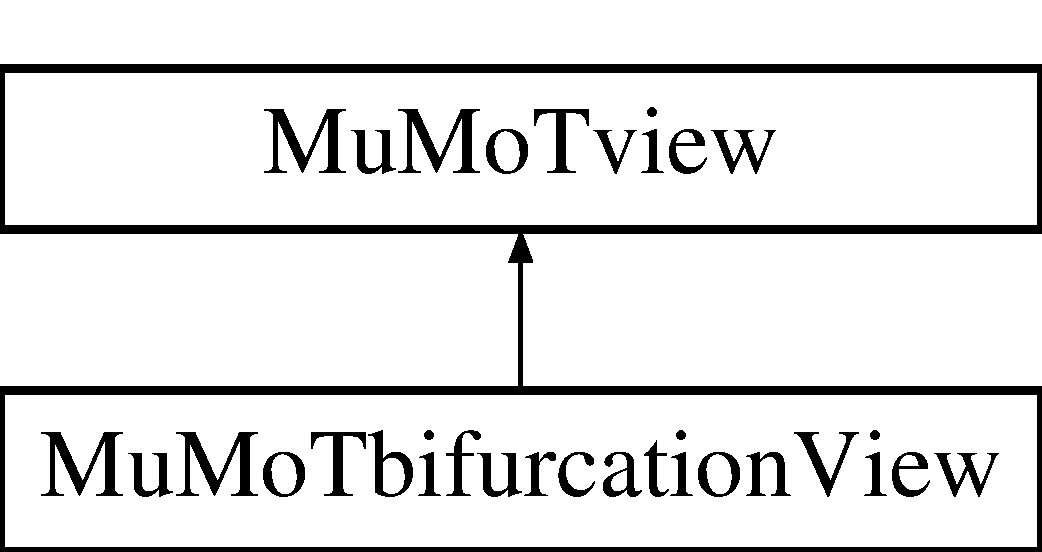
\includegraphics[height=2.000000cm]{class_mu_mo_t_1_1_mu_mo_t_1_1_mu_mo_tbifurcation_view}
\end{center}
\end{figure}
\subsection*{Public Member Functions}
\begin{DoxyCompactItemize}
\item 
def \hyperlink{class_mu_mo_t_1_1_mu_mo_t_1_1_mu_mo_tbifurcation_view_ac1764fc6547304e629425a5329dc7083}{\+\_\+\+\_\+init\+\_\+\+\_\+} (self, model, controller, bifurcation\+Parameter, state\+Variable1, state\+Variable2=\hyperlink{class_mu_mo_t_1_1_mu_mo_t_1_1_mu_mo_tbifurcation_view_ac7485dcc8d256a6f197ed7802687f252}{None}, \hyperlink{class_mu_mo_t_1_1_mu_mo_t_1_1_mu_mo_tbifurcation_view_a391e34f2de441d79152a7b3d6e4c9c86}{figure}=\hyperlink{class_mu_mo_t_1_1_mu_mo_t_1_1_mu_mo_tbifurcation_view_ac7485dcc8d256a6f197ed7802687f252}{None}, params=\hyperlink{class_mu_mo_t_1_1_mu_mo_t_1_1_mu_mo_tbifurcation_view_ac7485dcc8d256a6f197ed7802687f252}{None}, kwargs)
\end{DoxyCompactItemize}
\subsection*{Static Public Attributes}
\begin{DoxyCompactItemize}
\item 
dictionary \hyperlink{class_mu_mo_t_1_1_mu_mo_t_1_1_mu_mo_tbifurcation_view_a23ca095d6146b220be161f1f73017674}{initconds} = \{state\+Variable1\+: self.\+\_\+py\+D\+Smodel.\+pars\mbox{[}self.\+\_\+pydstoolify(self.\+\_\+mumot\+Model.\+\_\+system\+Size)\mbox{]} / len(self.\+\_\+mumot\+Model.\+\_\+reactants)\}
\item 
\hyperlink{class_mu_mo_t_1_1_mu_mo_t_1_1_mu_mo_tbifurcation_view_a08c7b0edb053705a8c47fe487b6f53bd}{ics}
\item 
\hyperlink{class_mu_mo_t_1_1_mu_mo_t_1_1_mu_mo_tbifurcation_view_a372cc7d4f485e77e35668d40b507d0e5}{pars}
\item 
\hyperlink{class_mu_mo_t_1_1_mu_mo_t_1_1_mu_mo_tbifurcation_view_ab74e6bf80237ddc4109968cedc58c151}{name}
\item 
\hyperlink{class_mu_mo_t_1_1_mu_mo_t_1_1_mu_mo_tbifurcation_view_a7aead736a07eaf25623ad7bfa1f0ee2d}{type}
\item 
\hyperlink{class_mu_mo_t_1_1_mu_mo_t_1_1_mu_mo_tbifurcation_view_a15cf90b3888db001a8299a477d50af98}{freepars}
\item 
\hyperlink{class_mu_mo_t_1_1_mu_mo_t_1_1_mu_mo_tbifurcation_view_aaa677c130e36435865b68ff6230a932d}{Max\+Num\+Points}
\item 
\hyperlink{class_mu_mo_t_1_1_mu_mo_t_1_1_mu_mo_tbifurcation_view_a0a7557ffe670b6a318afa8bd9851d2fc}{Max\+Step\+Size}
\begin{DoxyCompactList}\small\item\em The following 3 parameters are set after trial-\/and-\/error. \end{DoxyCompactList}\item 
\hyperlink{class_mu_mo_t_1_1_mu_mo_t_1_1_mu_mo_tbifurcation_view_a5fe506ca005e76a55ccd505a36e17fe6}{Min\+Step\+Size}
\item 
\hyperlink{class_mu_mo_t_1_1_mu_mo_t_1_1_mu_mo_tbifurcation_view_a9c25479455e9bdd389f37c4bccfefea1}{Step\+Size}
\item 
\hyperlink{class_mu_mo_t_1_1_mu_mo_t_1_1_mu_mo_tbifurcation_view_a7ff5325c1fceeebd63c3e4805a2206c8}{Loc\+Bif\+Points}
\item 
\hyperlink{class_mu_mo_t_1_1_mu_mo_t_1_1_mu_mo_tbifurcation_view_a040a7ecbcbaca807aeaec6d5c81801d5}{Save\+Eigen}
\item 
int \hyperlink{class_mu_mo_t_1_1_mu_mo_t_1_1_mu_mo_tbifurcation_view_a9ef495f853c90bcdd0b87dafa9480956}{k\+\_\+iter} = 1
\item 
\hyperlink{class_mu_mo_t_1_1_mu_mo_t_1_1_mu_mo_tbifurcation_view_a0ca47b3c8f2f64722024cb08752d8827}{s\+Points\+\_\+X}
\item 
\hyperlink{class_mu_mo_t_1_1_mu_mo_t_1_1_mu_mo_tbifurcation_view_aaaf9e21d7dbb0d83b922679ddcd42139}{s\+Points\+\_\+Y}
\item 
\hyperlink{class_mu_mo_t_1_1_mu_mo_t_1_1_mu_mo_tbifurcation_view_ad39e57ce255c4e1fd563afb4800468c3}{s\+Points\+\_\+\+Labels}
\item 
\hyperlink{class_mu_mo_t_1_1_mu_mo_t_1_1_mu_mo_tbifurcation_view_a64d4bfcc430575833bb5e2fbbba6d0ac}{s\+Points\+\_\+Z}
\item 
\hyperlink{class_mu_mo_t_1_1_mu_mo_t_1_1_mu_mo_tbifurcation_view_a3b8f497bab06dd2e00961fa7bd3a660c}{xdata}
\item 
\hyperlink{class_mu_mo_t_1_1_mu_mo_t_1_1_mu_mo_tbifurcation_view_aafaefd95e20265831bf905d93c40d87e}{ydata}
\item 
\hyperlink{class_mu_mo_t_1_1_mu_mo_t_1_1_mu_mo_tbifurcation_view_abb76a7390100209788848dbd6bb9fe30}{xlab}
\item 
\hyperlink{class_mu_mo_t_1_1_mu_mo_t_1_1_mu_mo_tbifurcation_view_a83433d4e45c13afe9a0042ae113ad169}{ylab}
\item 
\hyperlink{class_mu_mo_t_1_1_mu_mo_t_1_1_mu_mo_tbifurcation_view_a3c1c635ffc7ed4d381b8c672ebfac0fb}{special\+Points}
\item 
\hyperlink{class_mu_mo_t_1_1_mu_mo_t_1_1_mu_mo_tbifurcation_view_aa4c73e042e5fc54d56298cdbbba8e6c2}{eigenvalues}
\item 
\hyperlink{class_mu_mo_t_1_1_mu_mo_t_1_1_mu_mo_tbifurcation_view_a73c8f7f0d9593ed55a0cb1bea896b9f4}{ax\+\_\+reformat}
\item 
\hyperlink{class_mu_mo_t_1_1_mu_mo_t_1_1_mu_mo_tbifurcation_view_a36cde68b055f3f2ee671020af4ccf4e2}{False}
\item 
\hyperlink{class_mu_mo_t_1_1_mu_mo_t_1_1_mu_mo_tbifurcation_view_ac0e79460ed856ea3d8c366409bfe66e7}{curve\+\_\+replot}
\item 
\hyperlink{class_mu_mo_t_1_1_mu_mo_t_1_1_mu_mo_tbifurcation_view_a250a5d2f03fc812bbbbe6311276875f5}{fontsize}
\item 
\hyperlink{class_mu_mo_t_1_1_mu_mo_t_1_1_mu_mo_tbifurcation_view_addecde06ced656af71c7c68c4e780fe8}{axes}
\item 
\hyperlink{class_mu_mo_t_1_1_mu_mo_t_1_1_mu_mo_tbifurcation_view_ac7485dcc8d256a6f197ed7802687f252}{None}
\item 
\hyperlink{class_mu_mo_t_1_1_mu_mo_t_1_1_mu_mo_tbifurcation_view_a1df8fcdacfec00fc258a3c72772c2f18}{stability}
\item 
\hyperlink{class_mu_mo_t_1_1_mu_mo_t_1_1_mu_mo_tbifurcation_view_a643a20c0c59588a0f741a6095e2025fd}{True}
\item 
\hyperlink{class_mu_mo_t_1_1_mu_mo_t_1_1_mu_mo_tbifurcation_view_a391e34f2de441d79152a7b3d6e4c9c86}{figure}
\end{DoxyCompactItemize}
\subsection*{Private Member Functions}
\begin{DoxyCompactItemize}
\item 
def \hyperlink{class_mu_mo_t_1_1_mu_mo_t_1_1_mu_mo_tbifurcation_view_a385e5f82733060fec5122635ae6a8e67}{\+\_\+plot\+\_\+bifurcation} (self)
\item 
def \hyperlink{class_mu_mo_t_1_1_mu_mo_t_1_1_mu_mo_tbifurcation_view_a13b207330e0a4fe5bb7c3b863bbd0820}{\+\_\+replot\+\_\+bifurcation} (self)
\end{DoxyCompactItemize}
\subsection*{Private Attributes}
\begin{DoxyCompactItemize}
\item 
\hyperlink{class_mu_mo_t_1_1_mu_mo_t_1_1_mu_mo_tbifurcation_view_ace48ed03490093d8f44cde91e2f1e86e}{\+\_\+generating\+Command}
\item 
\hyperlink{class_mu_mo_t_1_1_mu_mo_t_1_1_mu_mo_tbifurcation_view_a6a353a1ef9443ae375948d592ed6cec6}{\+\_\+choose\+Font\+Size}
\item 
\hyperlink{class_mu_mo_t_1_1_mu_mo_t_1_1_mu_mo_tbifurcation_view_a865b2109ba10d874e84d4a354873b121}{\+\_\+xlab}
\item 
\hyperlink{class_mu_mo_t_1_1_mu_mo_t_1_1_mu_mo_tbifurcation_view_aac1a25a634d53e524573f67eb5f3a7b9}{\+\_\+ylab}
\item 
\hyperlink{class_mu_mo_t_1_1_mu_mo_t_1_1_mu_mo_tbifurcation_view_a16ef7868ecc22fd59dcacbb01e743f80}{\+\_\+bif\+Init}
\item 
\hyperlink{class_mu_mo_t_1_1_mu_mo_t_1_1_mu_mo_tbifurcation_view_a5c3de6779b1f8c64730cee48ca65491d}{\+\_\+init\+SV}
\end{DoxyCompactItemize}
\subsection*{Static Private Attributes}
\begin{DoxyCompactItemize}
\item 
\hyperlink{class_mu_mo_t_1_1_mu_mo_t_1_1_mu_mo_tbifurcation_view_a9e9a430da6d323cc4411c070e0c7eee5}{\+\_\+py\+D\+Smodel} = \hyperlink{class_mu_mo_t_1_1_mu_mo_t_1_1_mu_mo_tbifurcation_view_ac7485dcc8d256a6f197ed7802687f252}{None}
\item 
\hyperlink{class_mu_mo_t_1_1_mu_mo_t_1_1_mu_mo_tbifurcation_view_a17d5bd0e623faea6f50fc3b7f01d0d38}{\+\_\+bifurcation\+Parameter} = \hyperlink{class_mu_mo_t_1_1_mu_mo_t_1_1_mu_mo_tbifurcation_view_ac7485dcc8d256a6f197ed7802687f252}{None}
\begin{DoxyCompactList}\small\item\em 3-\/d bifurcation diagram ( \end{DoxyCompactList}\item 
\hyperlink{class_mu_mo_t_1_1_mu_mo_t_1_1_mu_mo_tbifurcation_view_aa14fa36730691becc6f3136899545416}{\+\_\+state\+Variable1} = \hyperlink{class_mu_mo_t_1_1_mu_mo_t_1_1_mu_mo_tbifurcation_view_ac7485dcc8d256a6f197ed7802687f252}{None}
\item 
\hyperlink{class_mu_mo_t_1_1_mu_mo_t_1_1_mu_mo_tbifurcation_view_a9d3705d1d9182e10751ff693573d6d16}{\+\_\+state\+Variable2} = \hyperlink{class_mu_mo_t_1_1_mu_mo_t_1_1_mu_mo_tbifurcation_view_ac7485dcc8d256a6f197ed7802687f252}{None}
\item 
\hyperlink{class_mu_mo_t_1_1_mu_mo_t_1_1_mu_mo_tbifurcation_view_a72e3294250042322910555edb2ef8f9d}{\+\_\+plotting\+Method} = \hyperlink{class_mu_mo_t_1_1_mu_mo_t_1_1_mu_mo_tbifurcation_view_ac7485dcc8d256a6f197ed7802687f252}{None}
\begin{DoxyCompactList}\small\item\em Plotting method to use. \end{DoxyCompactList}\item 
\hyperlink{class_mu_mo_t_1_1_mu_mo_t_1_1_mu_mo_tbifurcation_view_a1ae22852e6ebc2a6b1cdfee3383063e9}{\+\_\+\+LabelX}
\item 
\hyperlink{class_mu_mo_t_1_1_mu_mo_t_1_1_mu_mo_tbifurcation_view_ae2c6b16828eec194022056d04af84f16}{\+\_\+\+LabelY}
\item 
\hyperlink{class_mu_mo_t_1_1_mu_mo_t_1_1_mu_mo_tbifurcation_view_a45f0a60363e440604d8e5b08930eb7b5}{\+\_\+py\+D\+Sode}
\item 
\hyperlink{class_mu_mo_t_1_1_mu_mo_t_1_1_mu_mo_tbifurcation_view_a797e92fe19ce2636a49bf1400a69fc49}{\+\_\+py\+D\+Scont}
\begin{DoxyCompactList}\small\item\em @todo remove magic number \end{DoxyCompactList}\item 
\hyperlink{class_mu_mo_t_1_1_mu_mo_t_1_1_mu_mo_tbifurcation_view_aa56e2cffc879be68fdec55f29334415c}{\+\_\+py\+D\+Scont\+Args}
\item 
\hyperlink{class_mu_mo_t_1_1_mu_mo_t_1_1_mu_mo_tbifurcation_view_a0b40fc612e7c7203adf3274967cdd2ab}{\+\_\+special\+Points}
\begin{DoxyCompactList}\small\item\em use internal plotting routines\+: now supported! self.\+\_\+state\+Variable2 == None\+: 2-\/d bifurcation diagram \end{DoxyCompactList}\item 
\hyperlink{class_mu_mo_t_1_1_mu_mo_t_1_1_mu_mo_tbifurcation_view_a225ffda570ae3d9d5675af2fe28c1cbe}{\+\_\+\+Y\+D\+A\+TA}
\end{DoxyCompactItemize}


\subsection{Detailed Description}
bifurcation view on model 

\subsection{Constructor \& Destructor Documentation}
\mbox{\Hypertarget{class_mu_mo_t_1_1_mu_mo_t_1_1_mu_mo_tbifurcation_view_ac1764fc6547304e629425a5329dc7083}\label{class_mu_mo_t_1_1_mu_mo_t_1_1_mu_mo_tbifurcation_view_ac1764fc6547304e629425a5329dc7083}} 
\index{Mu\+Mo\+T\+::\+Mu\+Mo\+T\+::\+Mu\+Mo\+Tbifurcation\+View@{Mu\+Mo\+T\+::\+Mu\+Mo\+T\+::\+Mu\+Mo\+Tbifurcation\+View}!\+\_\+\+\_\+init\+\_\+\+\_\+@{\+\_\+\+\_\+init\+\_\+\+\_\+}}
\index{\+\_\+\+\_\+init\+\_\+\+\_\+@{\+\_\+\+\_\+init\+\_\+\+\_\+}!Mu\+Mo\+T\+::\+Mu\+Mo\+T\+::\+Mu\+Mo\+Tbifurcation\+View@{Mu\+Mo\+T\+::\+Mu\+Mo\+T\+::\+Mu\+Mo\+Tbifurcation\+View}}
\subsubsection{\texorpdfstring{\+\_\+\+\_\+init\+\_\+\+\_\+()}{\_\_init\_\_()}}
{\footnotesize\ttfamily def \+\_\+\+\_\+init\+\_\+\+\_\+ (\begin{DoxyParamCaption}\item[{}]{self,  }\item[{}]{model,  }\item[{}]{controller,  }\item[{}]{bifurcation\+Parameter,  }\item[{}]{state\+Variable1,  }\item[{}]{state\+Variable2 = {\ttfamily \hyperlink{class_mu_mo_t_1_1_mu_mo_t_1_1_mu_mo_tbifurcation_view_ac7485dcc8d256a6f197ed7802687f252}{None}},  }\item[{}]{figure = {\ttfamily \hyperlink{class_mu_mo_t_1_1_mu_mo_t_1_1_mu_mo_tbifurcation_view_ac7485dcc8d256a6f197ed7802687f252}{None}},  }\item[{}]{params = {\ttfamily \hyperlink{class_mu_mo_t_1_1_mu_mo_t_1_1_mu_mo_tbifurcation_view_ac7485dcc8d256a6f197ed7802687f252}{None}},  }\item[{}]{kwargs }\end{DoxyParamCaption})}



\subsection{Member Function Documentation}
\mbox{\Hypertarget{class_mu_mo_t_1_1_mu_mo_t_1_1_mu_mo_tbifurcation_view_a385e5f82733060fec5122635ae6a8e67}\label{class_mu_mo_t_1_1_mu_mo_t_1_1_mu_mo_tbifurcation_view_a385e5f82733060fec5122635ae6a8e67}} 
\index{Mu\+Mo\+T\+::\+Mu\+Mo\+T\+::\+Mu\+Mo\+Tbifurcation\+View@{Mu\+Mo\+T\+::\+Mu\+Mo\+T\+::\+Mu\+Mo\+Tbifurcation\+View}!\+\_\+plot\+\_\+bifurcation@{\+\_\+plot\+\_\+bifurcation}}
\index{\+\_\+plot\+\_\+bifurcation@{\+\_\+plot\+\_\+bifurcation}!Mu\+Mo\+T\+::\+Mu\+Mo\+T\+::\+Mu\+Mo\+Tbifurcation\+View@{Mu\+Mo\+T\+::\+Mu\+Mo\+T\+::\+Mu\+Mo\+Tbifurcation\+View}}
\subsubsection{\texorpdfstring{\+\_\+plot\+\_\+bifurcation()}{\_plot\_bifurcation()}}
{\footnotesize\ttfamily def \+\_\+plot\+\_\+bifurcation (\begin{DoxyParamCaption}\item[{}]{self }\end{DoxyParamCaption})\hspace{0.3cm}{\ttfamily [private]}}

\mbox{\Hypertarget{class_mu_mo_t_1_1_mu_mo_t_1_1_mu_mo_tbifurcation_view_a13b207330e0a4fe5bb7c3b863bbd0820}\label{class_mu_mo_t_1_1_mu_mo_t_1_1_mu_mo_tbifurcation_view_a13b207330e0a4fe5bb7c3b863bbd0820}} 
\index{Mu\+Mo\+T\+::\+Mu\+Mo\+T\+::\+Mu\+Mo\+Tbifurcation\+View@{Mu\+Mo\+T\+::\+Mu\+Mo\+T\+::\+Mu\+Mo\+Tbifurcation\+View}!\+\_\+replot\+\_\+bifurcation@{\+\_\+replot\+\_\+bifurcation}}
\index{\+\_\+replot\+\_\+bifurcation@{\+\_\+replot\+\_\+bifurcation}!Mu\+Mo\+T\+::\+Mu\+Mo\+T\+::\+Mu\+Mo\+Tbifurcation\+View@{Mu\+Mo\+T\+::\+Mu\+Mo\+T\+::\+Mu\+Mo\+Tbifurcation\+View}}
\subsubsection{\texorpdfstring{\+\_\+replot\+\_\+bifurcation()}{\_replot\_bifurcation()}}
{\footnotesize\ttfamily def \+\_\+replot\+\_\+bifurcation (\begin{DoxyParamCaption}\item[{}]{self }\end{DoxyParamCaption})\hspace{0.3cm}{\ttfamily [private]}}



\subsection{Field Documentation}
\mbox{\Hypertarget{class_mu_mo_t_1_1_mu_mo_t_1_1_mu_mo_tbifurcation_view_a16ef7868ecc22fd59dcacbb01e743f80}\label{class_mu_mo_t_1_1_mu_mo_t_1_1_mu_mo_tbifurcation_view_a16ef7868ecc22fd59dcacbb01e743f80}} 
\index{Mu\+Mo\+T\+::\+Mu\+Mo\+T\+::\+Mu\+Mo\+Tbifurcation\+View@{Mu\+Mo\+T\+::\+Mu\+Mo\+T\+::\+Mu\+Mo\+Tbifurcation\+View}!\+\_\+bif\+Init@{\+\_\+bif\+Init}}
\index{\+\_\+bif\+Init@{\+\_\+bif\+Init}!Mu\+Mo\+T\+::\+Mu\+Mo\+T\+::\+Mu\+Mo\+Tbifurcation\+View@{Mu\+Mo\+T\+::\+Mu\+Mo\+T\+::\+Mu\+Mo\+Tbifurcation\+View}}
\subsubsection{\texorpdfstring{\+\_\+bif\+Init}{\_bifInit}}
{\footnotesize\ttfamily \+\_\+bif\+Init\hspace{0.3cm}{\ttfamily [private]}}

\mbox{\Hypertarget{class_mu_mo_t_1_1_mu_mo_t_1_1_mu_mo_tbifurcation_view_a17d5bd0e623faea6f50fc3b7f01d0d38}\label{class_mu_mo_t_1_1_mu_mo_t_1_1_mu_mo_tbifurcation_view_a17d5bd0e623faea6f50fc3b7f01d0d38}} 
\index{Mu\+Mo\+T\+::\+Mu\+Mo\+T\+::\+Mu\+Mo\+Tbifurcation\+View@{Mu\+Mo\+T\+::\+Mu\+Mo\+T\+::\+Mu\+Mo\+Tbifurcation\+View}!\+\_\+bifurcation\+Parameter@{\+\_\+bifurcation\+Parameter}}
\index{\+\_\+bifurcation\+Parameter@{\+\_\+bifurcation\+Parameter}!Mu\+Mo\+T\+::\+Mu\+Mo\+T\+::\+Mu\+Mo\+Tbifurcation\+View@{Mu\+Mo\+T\+::\+Mu\+Mo\+T\+::\+Mu\+Mo\+Tbifurcation\+View}}
\subsubsection{\texorpdfstring{\+\_\+bifurcation\+Parameter}{\_bifurcationParameter}}
{\footnotesize\ttfamily \+\_\+bifurcation\+Parameter = \hyperlink{class_mu_mo_t_1_1_mu_mo_t_1_1_mu_mo_tbifurcation_view_ac7485dcc8d256a6f197ed7802687f252}{None}\hspace{0.3cm}{\ttfamily [static]}, {\ttfamily [private]}}



3-\/d bifurcation diagram ( 

\begin{DoxyRefDesc}{Todo}
\item[\hyperlink{todo__todo000047}{Todo}]\+: currently unsupported) \end{DoxyRefDesc}
\mbox{\Hypertarget{class_mu_mo_t_1_1_mu_mo_t_1_1_mu_mo_tbifurcation_view_a6a353a1ef9443ae375948d592ed6cec6}\label{class_mu_mo_t_1_1_mu_mo_t_1_1_mu_mo_tbifurcation_view_a6a353a1ef9443ae375948d592ed6cec6}} 
\index{Mu\+Mo\+T\+::\+Mu\+Mo\+T\+::\+Mu\+Mo\+Tbifurcation\+View@{Mu\+Mo\+T\+::\+Mu\+Mo\+T\+::\+Mu\+Mo\+Tbifurcation\+View}!\+\_\+choose\+Font\+Size@{\+\_\+choose\+Font\+Size}}
\index{\+\_\+choose\+Font\+Size@{\+\_\+choose\+Font\+Size}!Mu\+Mo\+T\+::\+Mu\+Mo\+T\+::\+Mu\+Mo\+Tbifurcation\+View@{Mu\+Mo\+T\+::\+Mu\+Mo\+T\+::\+Mu\+Mo\+Tbifurcation\+View}}
\subsubsection{\texorpdfstring{\+\_\+choose\+Font\+Size}{\_chooseFontSize}}
{\footnotesize\ttfamily \+\_\+choose\+Font\+Size\hspace{0.3cm}{\ttfamily [private]}}

\begin{DoxyRefDesc}{Todo}
\item[\hyperlink{todo__todo000051}{Todo}]was 1 (choose initial values sensibly) \end{DoxyRefDesc}
\begin{DoxyRefDesc}{Todo}
\item[\hyperlink{todo__todo000052}{Todo}]choose limit values sensibly \end{DoxyRefDesc}
\begin{DoxyRefDesc}{Todo}
\item[\hyperlink{todo__todo000053}{Todo}]choose rate step sensibly \end{DoxyRefDesc}
\begin{DoxyRefDesc}{Todo}
\item[\hyperlink{todo__todo000054}{Todo}]choose initial values sensibly \end{DoxyRefDesc}
\begin{DoxyRefDesc}{Todo}
\item[\hyperlink{todo__todo000055}{Todo}]choose system size sensibly \end{DoxyRefDesc}
\mbox{\Hypertarget{class_mu_mo_t_1_1_mu_mo_t_1_1_mu_mo_tbifurcation_view_ace48ed03490093d8f44cde91e2f1e86e}\label{class_mu_mo_t_1_1_mu_mo_t_1_1_mu_mo_tbifurcation_view_ace48ed03490093d8f44cde91e2f1e86e}} 
\index{Mu\+Mo\+T\+::\+Mu\+Mo\+T\+::\+Mu\+Mo\+Tbifurcation\+View@{Mu\+Mo\+T\+::\+Mu\+Mo\+T\+::\+Mu\+Mo\+Tbifurcation\+View}!\+\_\+generating\+Command@{\+\_\+generating\+Command}}
\index{\+\_\+generating\+Command@{\+\_\+generating\+Command}!Mu\+Mo\+T\+::\+Mu\+Mo\+T\+::\+Mu\+Mo\+Tbifurcation\+View@{Mu\+Mo\+T\+::\+Mu\+Mo\+T\+::\+Mu\+Mo\+Tbifurcation\+View}}
\subsubsection{\texorpdfstring{\+\_\+generating\+Command}{\_generatingCommand}}
{\footnotesize\ttfamily \+\_\+generating\+Command\hspace{0.3cm}{\ttfamily [private]}}

\mbox{\Hypertarget{class_mu_mo_t_1_1_mu_mo_t_1_1_mu_mo_tbifurcation_view_a5c3de6779b1f8c64730cee48ca65491d}\label{class_mu_mo_t_1_1_mu_mo_t_1_1_mu_mo_tbifurcation_view_a5c3de6779b1f8c64730cee48ca65491d}} 
\index{Mu\+Mo\+T\+::\+Mu\+Mo\+T\+::\+Mu\+Mo\+Tbifurcation\+View@{Mu\+Mo\+T\+::\+Mu\+Mo\+T\+::\+Mu\+Mo\+Tbifurcation\+View}!\+\_\+init\+SV@{\+\_\+init\+SV}}
\index{\+\_\+init\+SV@{\+\_\+init\+SV}!Mu\+Mo\+T\+::\+Mu\+Mo\+T\+::\+Mu\+Mo\+Tbifurcation\+View@{Mu\+Mo\+T\+::\+Mu\+Mo\+T\+::\+Mu\+Mo\+Tbifurcation\+View}}
\subsubsection{\texorpdfstring{\+\_\+init\+SV}{\_initSV}}
{\footnotesize\ttfamily \+\_\+init\+SV\hspace{0.3cm}{\ttfamily [private]}}

\mbox{\Hypertarget{class_mu_mo_t_1_1_mu_mo_t_1_1_mu_mo_tbifurcation_view_a1ae22852e6ebc2a6b1cdfee3383063e9}\label{class_mu_mo_t_1_1_mu_mo_t_1_1_mu_mo_tbifurcation_view_a1ae22852e6ebc2a6b1cdfee3383063e9}} 
\index{Mu\+Mo\+T\+::\+Mu\+Mo\+T\+::\+Mu\+Mo\+Tbifurcation\+View@{Mu\+Mo\+T\+::\+Mu\+Mo\+T\+::\+Mu\+Mo\+Tbifurcation\+View}!\+\_\+\+LabelX@{\+\_\+\+LabelX}}
\index{\+\_\+\+LabelX@{\+\_\+\+LabelX}!Mu\+Mo\+T\+::\+Mu\+Mo\+T\+::\+Mu\+Mo\+Tbifurcation\+View@{Mu\+Mo\+T\+::\+Mu\+Mo\+T\+::\+Mu\+Mo\+Tbifurcation\+View}}
\subsubsection{\texorpdfstring{\+\_\+\+LabelX}{\_LabelX}}
{\footnotesize\ttfamily \+\_\+\+LabelX\hspace{0.3cm}{\ttfamily [static]}, {\ttfamily [private]}}

\mbox{\Hypertarget{class_mu_mo_t_1_1_mu_mo_t_1_1_mu_mo_tbifurcation_view_ae2c6b16828eec194022056d04af84f16}\label{class_mu_mo_t_1_1_mu_mo_t_1_1_mu_mo_tbifurcation_view_ae2c6b16828eec194022056d04af84f16}} 
\index{Mu\+Mo\+T\+::\+Mu\+Mo\+T\+::\+Mu\+Mo\+Tbifurcation\+View@{Mu\+Mo\+T\+::\+Mu\+Mo\+T\+::\+Mu\+Mo\+Tbifurcation\+View}!\+\_\+\+LabelY@{\+\_\+\+LabelY}}
\index{\+\_\+\+LabelY@{\+\_\+\+LabelY}!Mu\+Mo\+T\+::\+Mu\+Mo\+T\+::\+Mu\+Mo\+Tbifurcation\+View@{Mu\+Mo\+T\+::\+Mu\+Mo\+T\+::\+Mu\+Mo\+Tbifurcation\+View}}
\subsubsection{\texorpdfstring{\+\_\+\+LabelY}{\_LabelY}}
{\footnotesize\ttfamily \+\_\+\+LabelY\hspace{0.3cm}{\ttfamily [static]}, {\ttfamily [private]}}

\mbox{\Hypertarget{class_mu_mo_t_1_1_mu_mo_t_1_1_mu_mo_tbifurcation_view_a72e3294250042322910555edb2ef8f9d}\label{class_mu_mo_t_1_1_mu_mo_t_1_1_mu_mo_tbifurcation_view_a72e3294250042322910555edb2ef8f9d}} 
\index{Mu\+Mo\+T\+::\+Mu\+Mo\+T\+::\+Mu\+Mo\+Tbifurcation\+View@{Mu\+Mo\+T\+::\+Mu\+Mo\+T\+::\+Mu\+Mo\+Tbifurcation\+View}!\+\_\+plotting\+Method@{\+\_\+plotting\+Method}}
\index{\+\_\+plotting\+Method@{\+\_\+plotting\+Method}!Mu\+Mo\+T\+::\+Mu\+Mo\+T\+::\+Mu\+Mo\+Tbifurcation\+View@{Mu\+Mo\+T\+::\+Mu\+Mo\+T\+::\+Mu\+Mo\+Tbifurcation\+View}}
\subsubsection{\texorpdfstring{\+\_\+plotting\+Method}{\_plottingMethod}}
{\footnotesize\ttfamily \+\_\+plotting\+Method = \hyperlink{class_mu_mo_t_1_1_mu_mo_t_1_1_mu_mo_tbifurcation_view_ac7485dcc8d256a6f197ed7802687f252}{None}\hspace{0.3cm}{\ttfamily [static]}, {\ttfamily [private]}}



Plotting method to use. 

\mbox{\Hypertarget{class_mu_mo_t_1_1_mu_mo_t_1_1_mu_mo_tbifurcation_view_a797e92fe19ce2636a49bf1400a69fc49}\label{class_mu_mo_t_1_1_mu_mo_t_1_1_mu_mo_tbifurcation_view_a797e92fe19ce2636a49bf1400a69fc49}} 
\index{Mu\+Mo\+T\+::\+Mu\+Mo\+T\+::\+Mu\+Mo\+Tbifurcation\+View@{Mu\+Mo\+T\+::\+Mu\+Mo\+T\+::\+Mu\+Mo\+Tbifurcation\+View}!\+\_\+py\+D\+Scont@{\+\_\+py\+D\+Scont}}
\index{\+\_\+py\+D\+Scont@{\+\_\+py\+D\+Scont}!Mu\+Mo\+T\+::\+Mu\+Mo\+T\+::\+Mu\+Mo\+Tbifurcation\+View@{Mu\+Mo\+T\+::\+Mu\+Mo\+T\+::\+Mu\+Mo\+Tbifurcation\+View}}
\subsubsection{\texorpdfstring{\+\_\+py\+D\+Scont}{\_pyDScont}}
{\footnotesize\ttfamily \+\_\+py\+D\+Scont\hspace{0.3cm}{\ttfamily [static]}, {\ttfamily [private]}}



@todo remove magic number 

\begin{DoxyRefDesc}{Todo}
\item[\hyperlink{todo__todo000058}{Todo}]\+: add to {\bfseries init}() \end{DoxyRefDesc}
\begin{DoxyRefDesc}{Todo}
\item[\hyperlink{todo__todo000059}{Todo}]remove magic number \end{DoxyRefDesc}
\mbox{\Hypertarget{class_mu_mo_t_1_1_mu_mo_t_1_1_mu_mo_tbifurcation_view_aa56e2cffc879be68fdec55f29334415c}\label{class_mu_mo_t_1_1_mu_mo_t_1_1_mu_mo_tbifurcation_view_aa56e2cffc879be68fdec55f29334415c}} 
\index{Mu\+Mo\+T\+::\+Mu\+Mo\+T\+::\+Mu\+Mo\+Tbifurcation\+View@{Mu\+Mo\+T\+::\+Mu\+Mo\+T\+::\+Mu\+Mo\+Tbifurcation\+View}!\+\_\+py\+D\+Scont\+Args@{\+\_\+py\+D\+Scont\+Args}}
\index{\+\_\+py\+D\+Scont\+Args@{\+\_\+py\+D\+Scont\+Args}!Mu\+Mo\+T\+::\+Mu\+Mo\+T\+::\+Mu\+Mo\+Tbifurcation\+View@{Mu\+Mo\+T\+::\+Mu\+Mo\+T\+::\+Mu\+Mo\+Tbifurcation\+View}}
\subsubsection{\texorpdfstring{\+\_\+py\+D\+Scont\+Args}{\_pyDScontArgs}}
{\footnotesize\ttfamily \+\_\+py\+D\+Scont\+Args\hspace{0.3cm}{\ttfamily [static]}, {\ttfamily [private]}}

\begin{DoxyRefDesc}{Todo}
\item[\hyperlink{todo__todo000048}{Todo}]\+: add self.\+\_\+py\+D\+Scont\+Args to {\bfseries init}() \end{DoxyRefDesc}
\mbox{\Hypertarget{class_mu_mo_t_1_1_mu_mo_t_1_1_mu_mo_tbifurcation_view_a9e9a430da6d323cc4411c070e0c7eee5}\label{class_mu_mo_t_1_1_mu_mo_t_1_1_mu_mo_tbifurcation_view_a9e9a430da6d323cc4411c070e0c7eee5}} 
\index{Mu\+Mo\+T\+::\+Mu\+Mo\+T\+::\+Mu\+Mo\+Tbifurcation\+View@{Mu\+Mo\+T\+::\+Mu\+Mo\+T\+::\+Mu\+Mo\+Tbifurcation\+View}!\+\_\+py\+D\+Smodel@{\+\_\+py\+D\+Smodel}}
\index{\+\_\+py\+D\+Smodel@{\+\_\+py\+D\+Smodel}!Mu\+Mo\+T\+::\+Mu\+Mo\+T\+::\+Mu\+Mo\+Tbifurcation\+View@{Mu\+Mo\+T\+::\+Mu\+Mo\+T\+::\+Mu\+Mo\+Tbifurcation\+View}}
\subsubsection{\texorpdfstring{\+\_\+py\+D\+Smodel}{\_pyDSmodel}}
{\footnotesize\ttfamily \+\_\+py\+D\+Smodel = \hyperlink{class_mu_mo_t_1_1_mu_mo_t_1_1_mu_mo_tbifurcation_view_ac7485dcc8d256a6f197ed7802687f252}{None}\hspace{0.3cm}{\ttfamily [static]}, {\ttfamily [private]}}

\mbox{\Hypertarget{class_mu_mo_t_1_1_mu_mo_t_1_1_mu_mo_tbifurcation_view_a45f0a60363e440604d8e5b08930eb7b5}\label{class_mu_mo_t_1_1_mu_mo_t_1_1_mu_mo_tbifurcation_view_a45f0a60363e440604d8e5b08930eb7b5}} 
\index{Mu\+Mo\+T\+::\+Mu\+Mo\+T\+::\+Mu\+Mo\+Tbifurcation\+View@{Mu\+Mo\+T\+::\+Mu\+Mo\+T\+::\+Mu\+Mo\+Tbifurcation\+View}!\+\_\+py\+D\+Sode@{\+\_\+py\+D\+Sode}}
\index{\+\_\+py\+D\+Sode@{\+\_\+py\+D\+Sode}!Mu\+Mo\+T\+::\+Mu\+Mo\+T\+::\+Mu\+Mo\+Tbifurcation\+View@{Mu\+Mo\+T\+::\+Mu\+Mo\+T\+::\+Mu\+Mo\+Tbifurcation\+View}}
\subsubsection{\texorpdfstring{\+\_\+py\+D\+Sode}{\_pyDSode}}
{\footnotesize\ttfamily \+\_\+py\+D\+Sode\hspace{0.3cm}{\ttfamily [static]}, {\ttfamily [private]}}

\mbox{\Hypertarget{class_mu_mo_t_1_1_mu_mo_t_1_1_mu_mo_tbifurcation_view_a0b40fc612e7c7203adf3274967cdd2ab}\label{class_mu_mo_t_1_1_mu_mo_t_1_1_mu_mo_tbifurcation_view_a0b40fc612e7c7203adf3274967cdd2ab}} 
\index{Mu\+Mo\+T\+::\+Mu\+Mo\+T\+::\+Mu\+Mo\+Tbifurcation\+View@{Mu\+Mo\+T\+::\+Mu\+Mo\+T\+::\+Mu\+Mo\+Tbifurcation\+View}!\+\_\+special\+Points@{\+\_\+special\+Points}}
\index{\+\_\+special\+Points@{\+\_\+special\+Points}!Mu\+Mo\+T\+::\+Mu\+Mo\+T\+::\+Mu\+Mo\+Tbifurcation\+View@{Mu\+Mo\+T\+::\+Mu\+Mo\+T\+::\+Mu\+Mo\+Tbifurcation\+View}}
\subsubsection{\texorpdfstring{\+\_\+special\+Points}{\_specialPoints}}
{\footnotesize\ttfamily \+\_\+special\+Points\hspace{0.3cm}{\ttfamily [static]}, {\ttfamily [private]}}



use internal plotting routines\+: now supported! self.\+\_\+state\+Variable2 == None\+: 2-\/d bifurcation diagram 

\mbox{\Hypertarget{class_mu_mo_t_1_1_mu_mo_t_1_1_mu_mo_tbifurcation_view_aa14fa36730691becc6f3136899545416}\label{class_mu_mo_t_1_1_mu_mo_t_1_1_mu_mo_tbifurcation_view_aa14fa36730691becc6f3136899545416}} 
\index{Mu\+Mo\+T\+::\+Mu\+Mo\+T\+::\+Mu\+Mo\+Tbifurcation\+View@{Mu\+Mo\+T\+::\+Mu\+Mo\+T\+::\+Mu\+Mo\+Tbifurcation\+View}!\+\_\+state\+Variable1@{\+\_\+state\+Variable1}}
\index{\+\_\+state\+Variable1@{\+\_\+state\+Variable1}!Mu\+Mo\+T\+::\+Mu\+Mo\+T\+::\+Mu\+Mo\+Tbifurcation\+View@{Mu\+Mo\+T\+::\+Mu\+Mo\+T\+::\+Mu\+Mo\+Tbifurcation\+View}}
\subsubsection{\texorpdfstring{\+\_\+state\+Variable1}{\_stateVariable1}}
{\footnotesize\ttfamily \+\_\+state\+Variable1 = \hyperlink{class_mu_mo_t_1_1_mu_mo_t_1_1_mu_mo_tbifurcation_view_ac7485dcc8d256a6f197ed7802687f252}{None}\hspace{0.3cm}{\ttfamily [static]}, {\ttfamily [private]}}

\mbox{\Hypertarget{class_mu_mo_t_1_1_mu_mo_t_1_1_mu_mo_tbifurcation_view_a9d3705d1d9182e10751ff693573d6d16}\label{class_mu_mo_t_1_1_mu_mo_t_1_1_mu_mo_tbifurcation_view_a9d3705d1d9182e10751ff693573d6d16}} 
\index{Mu\+Mo\+T\+::\+Mu\+Mo\+T\+::\+Mu\+Mo\+Tbifurcation\+View@{Mu\+Mo\+T\+::\+Mu\+Mo\+T\+::\+Mu\+Mo\+Tbifurcation\+View}!\+\_\+state\+Variable2@{\+\_\+state\+Variable2}}
\index{\+\_\+state\+Variable2@{\+\_\+state\+Variable2}!Mu\+Mo\+T\+::\+Mu\+Mo\+T\+::\+Mu\+Mo\+Tbifurcation\+View@{Mu\+Mo\+T\+::\+Mu\+Mo\+T\+::\+Mu\+Mo\+Tbifurcation\+View}}
\subsubsection{\texorpdfstring{\+\_\+state\+Variable2}{\_stateVariable2}}
{\footnotesize\ttfamily \+\_\+state\+Variable2 = \hyperlink{class_mu_mo_t_1_1_mu_mo_t_1_1_mu_mo_tbifurcation_view_ac7485dcc8d256a6f197ed7802687f252}{None}\hspace{0.3cm}{\ttfamily [static]}, {\ttfamily [private]}}

\mbox{\Hypertarget{class_mu_mo_t_1_1_mu_mo_t_1_1_mu_mo_tbifurcation_view_a865b2109ba10d874e84d4a354873b121}\label{class_mu_mo_t_1_1_mu_mo_t_1_1_mu_mo_tbifurcation_view_a865b2109ba10d874e84d4a354873b121}} 
\index{Mu\+Mo\+T\+::\+Mu\+Mo\+T\+::\+Mu\+Mo\+Tbifurcation\+View@{Mu\+Mo\+T\+::\+Mu\+Mo\+T\+::\+Mu\+Mo\+Tbifurcation\+View}!\+\_\+xlab@{\+\_\+xlab}}
\index{\+\_\+xlab@{\+\_\+xlab}!Mu\+Mo\+T\+::\+Mu\+Mo\+T\+::\+Mu\+Mo\+Tbifurcation\+View@{Mu\+Mo\+T\+::\+Mu\+Mo\+T\+::\+Mu\+Mo\+Tbifurcation\+View}}
\subsubsection{\texorpdfstring{\+\_\+xlab}{\_xlab}}
{\footnotesize\ttfamily \+\_\+xlab\hspace{0.3cm}{\ttfamily [private]}}

\mbox{\Hypertarget{class_mu_mo_t_1_1_mu_mo_t_1_1_mu_mo_tbifurcation_view_a225ffda570ae3d9d5675af2fe28c1cbe}\label{class_mu_mo_t_1_1_mu_mo_t_1_1_mu_mo_tbifurcation_view_a225ffda570ae3d9d5675af2fe28c1cbe}} 
\index{Mu\+Mo\+T\+::\+Mu\+Mo\+T\+::\+Mu\+Mo\+Tbifurcation\+View@{Mu\+Mo\+T\+::\+Mu\+Mo\+T\+::\+Mu\+Mo\+Tbifurcation\+View}!\+\_\+\+Y\+D\+A\+TA@{\+\_\+\+Y\+D\+A\+TA}}
\index{\+\_\+\+Y\+D\+A\+TA@{\+\_\+\+Y\+D\+A\+TA}!Mu\+Mo\+T\+::\+Mu\+Mo\+T\+::\+Mu\+Mo\+Tbifurcation\+View@{Mu\+Mo\+T\+::\+Mu\+Mo\+T\+::\+Mu\+Mo\+Tbifurcation\+View}}
\subsubsection{\texorpdfstring{\+\_\+\+Y\+D\+A\+TA}{\_YDATA}}
{\footnotesize\ttfamily \+\_\+\+Y\+D\+A\+TA\hspace{0.3cm}{\ttfamily [static]}, {\ttfamily [private]}}

\mbox{\Hypertarget{class_mu_mo_t_1_1_mu_mo_t_1_1_mu_mo_tbifurcation_view_aac1a25a634d53e524573f67eb5f3a7b9}\label{class_mu_mo_t_1_1_mu_mo_t_1_1_mu_mo_tbifurcation_view_aac1a25a634d53e524573f67eb5f3a7b9}} 
\index{Mu\+Mo\+T\+::\+Mu\+Mo\+T\+::\+Mu\+Mo\+Tbifurcation\+View@{Mu\+Mo\+T\+::\+Mu\+Mo\+T\+::\+Mu\+Mo\+Tbifurcation\+View}!\+\_\+ylab@{\+\_\+ylab}}
\index{\+\_\+ylab@{\+\_\+ylab}!Mu\+Mo\+T\+::\+Mu\+Mo\+T\+::\+Mu\+Mo\+Tbifurcation\+View@{Mu\+Mo\+T\+::\+Mu\+Mo\+T\+::\+Mu\+Mo\+Tbifurcation\+View}}
\subsubsection{\texorpdfstring{\+\_\+ylab}{\_ylab}}
{\footnotesize\ttfamily \+\_\+ylab\hspace{0.3cm}{\ttfamily [private]}}

\mbox{\Hypertarget{class_mu_mo_t_1_1_mu_mo_t_1_1_mu_mo_tbifurcation_view_a73c8f7f0d9593ed55a0cb1bea896b9f4}\label{class_mu_mo_t_1_1_mu_mo_t_1_1_mu_mo_tbifurcation_view_a73c8f7f0d9593ed55a0cb1bea896b9f4}} 
\index{Mu\+Mo\+T\+::\+Mu\+Mo\+T\+::\+Mu\+Mo\+Tbifurcation\+View@{Mu\+Mo\+T\+::\+Mu\+Mo\+T\+::\+Mu\+Mo\+Tbifurcation\+View}!ax\+\_\+reformat@{ax\+\_\+reformat}}
\index{ax\+\_\+reformat@{ax\+\_\+reformat}!Mu\+Mo\+T\+::\+Mu\+Mo\+T\+::\+Mu\+Mo\+Tbifurcation\+View@{Mu\+Mo\+T\+::\+Mu\+Mo\+T\+::\+Mu\+Mo\+Tbifurcation\+View}}
\subsubsection{\texorpdfstring{ax\+\_\+reformat}{ax\_reformat}}
{\footnotesize\ttfamily ax\+\_\+reformat\hspace{0.3cm}{\ttfamily [static]}}

\mbox{\Hypertarget{class_mu_mo_t_1_1_mu_mo_t_1_1_mu_mo_tbifurcation_view_addecde06ced656af71c7c68c4e780fe8}\label{class_mu_mo_t_1_1_mu_mo_t_1_1_mu_mo_tbifurcation_view_addecde06ced656af71c7c68c4e780fe8}} 
\index{Mu\+Mo\+T\+::\+Mu\+Mo\+T\+::\+Mu\+Mo\+Tbifurcation\+View@{Mu\+Mo\+T\+::\+Mu\+Mo\+T\+::\+Mu\+Mo\+Tbifurcation\+View}!axes@{axes}}
\index{axes@{axes}!Mu\+Mo\+T\+::\+Mu\+Mo\+T\+::\+Mu\+Mo\+Tbifurcation\+View@{Mu\+Mo\+T\+::\+Mu\+Mo\+T\+::\+Mu\+Mo\+Tbifurcation\+View}}
\subsubsection{\texorpdfstring{axes}{axes}}
{\footnotesize\ttfamily axes\hspace{0.3cm}{\ttfamily [static]}}

\mbox{\Hypertarget{class_mu_mo_t_1_1_mu_mo_t_1_1_mu_mo_tbifurcation_view_ac0e79460ed856ea3d8c366409bfe66e7}\label{class_mu_mo_t_1_1_mu_mo_t_1_1_mu_mo_tbifurcation_view_ac0e79460ed856ea3d8c366409bfe66e7}} 
\index{Mu\+Mo\+T\+::\+Mu\+Mo\+T\+::\+Mu\+Mo\+Tbifurcation\+View@{Mu\+Mo\+T\+::\+Mu\+Mo\+T\+::\+Mu\+Mo\+Tbifurcation\+View}!curve\+\_\+replot@{curve\+\_\+replot}}
\index{curve\+\_\+replot@{curve\+\_\+replot}!Mu\+Mo\+T\+::\+Mu\+Mo\+T\+::\+Mu\+Mo\+Tbifurcation\+View@{Mu\+Mo\+T\+::\+Mu\+Mo\+T\+::\+Mu\+Mo\+Tbifurcation\+View}}
\subsubsection{\texorpdfstring{curve\+\_\+replot}{curve\_replot}}
{\footnotesize\ttfamily curve\+\_\+replot\hspace{0.3cm}{\ttfamily [static]}}

\mbox{\Hypertarget{class_mu_mo_t_1_1_mu_mo_t_1_1_mu_mo_tbifurcation_view_aa4c73e042e5fc54d56298cdbbba8e6c2}\label{class_mu_mo_t_1_1_mu_mo_t_1_1_mu_mo_tbifurcation_view_aa4c73e042e5fc54d56298cdbbba8e6c2}} 
\index{Mu\+Mo\+T\+::\+Mu\+Mo\+T\+::\+Mu\+Mo\+Tbifurcation\+View@{Mu\+Mo\+T\+::\+Mu\+Mo\+T\+::\+Mu\+Mo\+Tbifurcation\+View}!eigenvalues@{eigenvalues}}
\index{eigenvalues@{eigenvalues}!Mu\+Mo\+T\+::\+Mu\+Mo\+T\+::\+Mu\+Mo\+Tbifurcation\+View@{Mu\+Mo\+T\+::\+Mu\+Mo\+T\+::\+Mu\+Mo\+Tbifurcation\+View}}
\subsubsection{\texorpdfstring{eigenvalues}{eigenvalues}}
{\footnotesize\ttfamily eigenvalues\hspace{0.3cm}{\ttfamily [static]}}

\mbox{\Hypertarget{class_mu_mo_t_1_1_mu_mo_t_1_1_mu_mo_tbifurcation_view_a36cde68b055f3f2ee671020af4ccf4e2}\label{class_mu_mo_t_1_1_mu_mo_t_1_1_mu_mo_tbifurcation_view_a36cde68b055f3f2ee671020af4ccf4e2}} 
\index{Mu\+Mo\+T\+::\+Mu\+Mo\+T\+::\+Mu\+Mo\+Tbifurcation\+View@{Mu\+Mo\+T\+::\+Mu\+Mo\+T\+::\+Mu\+Mo\+Tbifurcation\+View}!False@{False}}
\index{False@{False}!Mu\+Mo\+T\+::\+Mu\+Mo\+T\+::\+Mu\+Mo\+Tbifurcation\+View@{Mu\+Mo\+T\+::\+Mu\+Mo\+T\+::\+Mu\+Mo\+Tbifurcation\+View}}
\subsubsection{\texorpdfstring{False}{False}}
{\footnotesize\ttfamily False\hspace{0.3cm}{\ttfamily [static]}}

\mbox{\Hypertarget{class_mu_mo_t_1_1_mu_mo_t_1_1_mu_mo_tbifurcation_view_a391e34f2de441d79152a7b3d6e4c9c86}\label{class_mu_mo_t_1_1_mu_mo_t_1_1_mu_mo_tbifurcation_view_a391e34f2de441d79152a7b3d6e4c9c86}} 
\index{Mu\+Mo\+T\+::\+Mu\+Mo\+T\+::\+Mu\+Mo\+Tbifurcation\+View@{Mu\+Mo\+T\+::\+Mu\+Mo\+T\+::\+Mu\+Mo\+Tbifurcation\+View}!figure@{figure}}
\index{figure@{figure}!Mu\+Mo\+T\+::\+Mu\+Mo\+T\+::\+Mu\+Mo\+Tbifurcation\+View@{Mu\+Mo\+T\+::\+Mu\+Mo\+T\+::\+Mu\+Mo\+Tbifurcation\+View}}
\subsubsection{\texorpdfstring{figure}{figure}}
{\footnotesize\ttfamily figure\hspace{0.3cm}{\ttfamily [static]}}

\mbox{\Hypertarget{class_mu_mo_t_1_1_mu_mo_t_1_1_mu_mo_tbifurcation_view_a250a5d2f03fc812bbbbe6311276875f5}\label{class_mu_mo_t_1_1_mu_mo_t_1_1_mu_mo_tbifurcation_view_a250a5d2f03fc812bbbbe6311276875f5}} 
\index{Mu\+Mo\+T\+::\+Mu\+Mo\+T\+::\+Mu\+Mo\+Tbifurcation\+View@{Mu\+Mo\+T\+::\+Mu\+Mo\+T\+::\+Mu\+Mo\+Tbifurcation\+View}!fontsize@{fontsize}}
\index{fontsize@{fontsize}!Mu\+Mo\+T\+::\+Mu\+Mo\+T\+::\+Mu\+Mo\+Tbifurcation\+View@{Mu\+Mo\+T\+::\+Mu\+Mo\+T\+::\+Mu\+Mo\+Tbifurcation\+View}}
\subsubsection{\texorpdfstring{fontsize}{fontsize}}
{\footnotesize\ttfamily fontsize\hspace{0.3cm}{\ttfamily [static]}}

\mbox{\Hypertarget{class_mu_mo_t_1_1_mu_mo_t_1_1_mu_mo_tbifurcation_view_a15cf90b3888db001a8299a477d50af98}\label{class_mu_mo_t_1_1_mu_mo_t_1_1_mu_mo_tbifurcation_view_a15cf90b3888db001a8299a477d50af98}} 
\index{Mu\+Mo\+T\+::\+Mu\+Mo\+T\+::\+Mu\+Mo\+Tbifurcation\+View@{Mu\+Mo\+T\+::\+Mu\+Mo\+T\+::\+Mu\+Mo\+Tbifurcation\+View}!freepars@{freepars}}
\index{freepars@{freepars}!Mu\+Mo\+T\+::\+Mu\+Mo\+T\+::\+Mu\+Mo\+Tbifurcation\+View@{Mu\+Mo\+T\+::\+Mu\+Mo\+T\+::\+Mu\+Mo\+Tbifurcation\+View}}
\subsubsection{\texorpdfstring{freepars}{freepars}}
{\footnotesize\ttfamily freepars\hspace{0.3cm}{\ttfamily [static]}}

\mbox{\Hypertarget{class_mu_mo_t_1_1_mu_mo_t_1_1_mu_mo_tbifurcation_view_a08c7b0edb053705a8c47fe487b6f53bd}\label{class_mu_mo_t_1_1_mu_mo_t_1_1_mu_mo_tbifurcation_view_a08c7b0edb053705a8c47fe487b6f53bd}} 
\index{Mu\+Mo\+T\+::\+Mu\+Mo\+T\+::\+Mu\+Mo\+Tbifurcation\+View@{Mu\+Mo\+T\+::\+Mu\+Mo\+T\+::\+Mu\+Mo\+Tbifurcation\+View}!ics@{ics}}
\index{ics@{ics}!Mu\+Mo\+T\+::\+Mu\+Mo\+T\+::\+Mu\+Mo\+Tbifurcation\+View@{Mu\+Mo\+T\+::\+Mu\+Mo\+T\+::\+Mu\+Mo\+Tbifurcation\+View}}
\subsubsection{\texorpdfstring{ics}{ics}}
{\footnotesize\ttfamily ics\hspace{0.3cm}{\ttfamily [static]}}

\mbox{\Hypertarget{class_mu_mo_t_1_1_mu_mo_t_1_1_mu_mo_tbifurcation_view_a23ca095d6146b220be161f1f73017674}\label{class_mu_mo_t_1_1_mu_mo_t_1_1_mu_mo_tbifurcation_view_a23ca095d6146b220be161f1f73017674}} 
\index{Mu\+Mo\+T\+::\+Mu\+Mo\+T\+::\+Mu\+Mo\+Tbifurcation\+View@{Mu\+Mo\+T\+::\+Mu\+Mo\+T\+::\+Mu\+Mo\+Tbifurcation\+View}!initconds@{initconds}}
\index{initconds@{initconds}!Mu\+Mo\+T\+::\+Mu\+Mo\+T\+::\+Mu\+Mo\+Tbifurcation\+View@{Mu\+Mo\+T\+::\+Mu\+Mo\+T\+::\+Mu\+Mo\+Tbifurcation\+View}}
\subsubsection{\texorpdfstring{initconds}{initconds}}
{\footnotesize\ttfamily dictionary initconds = \{state\+Variable1\+: self.\+\_\+py\+D\+Smodel.\+pars\mbox{[}self.\+\_\+pydstoolify(self.\+\_\+mumot\+Model.\+\_\+system\+Size)\mbox{]} / len(self.\+\_\+mumot\+Model.\+\_\+reactants)\}\hspace{0.3cm}{\ttfamily [static]}}

\mbox{\Hypertarget{class_mu_mo_t_1_1_mu_mo_t_1_1_mu_mo_tbifurcation_view_a9ef495f853c90bcdd0b87dafa9480956}\label{class_mu_mo_t_1_1_mu_mo_t_1_1_mu_mo_tbifurcation_view_a9ef495f853c90bcdd0b87dafa9480956}} 
\index{Mu\+Mo\+T\+::\+Mu\+Mo\+T\+::\+Mu\+Mo\+Tbifurcation\+View@{Mu\+Mo\+T\+::\+Mu\+Mo\+T\+::\+Mu\+Mo\+Tbifurcation\+View}!k\+\_\+iter@{k\+\_\+iter}}
\index{k\+\_\+iter@{k\+\_\+iter}!Mu\+Mo\+T\+::\+Mu\+Mo\+T\+::\+Mu\+Mo\+Tbifurcation\+View@{Mu\+Mo\+T\+::\+Mu\+Mo\+T\+::\+Mu\+Mo\+Tbifurcation\+View}}
\subsubsection{\texorpdfstring{k\+\_\+iter}{k\_iter}}
{\footnotesize\ttfamily int k\+\_\+iter = 1\hspace{0.3cm}{\ttfamily [static]}}

\mbox{\Hypertarget{class_mu_mo_t_1_1_mu_mo_t_1_1_mu_mo_tbifurcation_view_a7ff5325c1fceeebd63c3e4805a2206c8}\label{class_mu_mo_t_1_1_mu_mo_t_1_1_mu_mo_tbifurcation_view_a7ff5325c1fceeebd63c3e4805a2206c8}} 
\index{Mu\+Mo\+T\+::\+Mu\+Mo\+T\+::\+Mu\+Mo\+Tbifurcation\+View@{Mu\+Mo\+T\+::\+Mu\+Mo\+T\+::\+Mu\+Mo\+Tbifurcation\+View}!Loc\+Bif\+Points@{Loc\+Bif\+Points}}
\index{Loc\+Bif\+Points@{Loc\+Bif\+Points}!Mu\+Mo\+T\+::\+Mu\+Mo\+T\+::\+Mu\+Mo\+Tbifurcation\+View@{Mu\+Mo\+T\+::\+Mu\+Mo\+T\+::\+Mu\+Mo\+Tbifurcation\+View}}
\subsubsection{\texorpdfstring{Loc\+Bif\+Points}{LocBifPoints}}
{\footnotesize\ttfamily Loc\+Bif\+Points\hspace{0.3cm}{\ttfamily [static]}}

\mbox{\Hypertarget{class_mu_mo_t_1_1_mu_mo_t_1_1_mu_mo_tbifurcation_view_aaa677c130e36435865b68ff6230a932d}\label{class_mu_mo_t_1_1_mu_mo_t_1_1_mu_mo_tbifurcation_view_aaa677c130e36435865b68ff6230a932d}} 
\index{Mu\+Mo\+T\+::\+Mu\+Mo\+T\+::\+Mu\+Mo\+Tbifurcation\+View@{Mu\+Mo\+T\+::\+Mu\+Mo\+T\+::\+Mu\+Mo\+Tbifurcation\+View}!Max\+Num\+Points@{Max\+Num\+Points}}
\index{Max\+Num\+Points@{Max\+Num\+Points}!Mu\+Mo\+T\+::\+Mu\+Mo\+T\+::\+Mu\+Mo\+Tbifurcation\+View@{Mu\+Mo\+T\+::\+Mu\+Mo\+T\+::\+Mu\+Mo\+Tbifurcation\+View}}
\subsubsection{\texorpdfstring{Max\+Num\+Points}{MaxNumPoints}}
{\footnotesize\ttfamily Max\+Num\+Points\hspace{0.3cm}{\ttfamily [static]}}

\mbox{\Hypertarget{class_mu_mo_t_1_1_mu_mo_t_1_1_mu_mo_tbifurcation_view_a0a7557ffe670b6a318afa8bd9851d2fc}\label{class_mu_mo_t_1_1_mu_mo_t_1_1_mu_mo_tbifurcation_view_a0a7557ffe670b6a318afa8bd9851d2fc}} 
\index{Mu\+Mo\+T\+::\+Mu\+Mo\+T\+::\+Mu\+Mo\+Tbifurcation\+View@{Mu\+Mo\+T\+::\+Mu\+Mo\+T\+::\+Mu\+Mo\+Tbifurcation\+View}!Max\+Step\+Size@{Max\+Step\+Size}}
\index{Max\+Step\+Size@{Max\+Step\+Size}!Mu\+Mo\+T\+::\+Mu\+Mo\+T\+::\+Mu\+Mo\+Tbifurcation\+View@{Mu\+Mo\+T\+::\+Mu\+Mo\+T\+::\+Mu\+Mo\+Tbifurcation\+View}}
\subsubsection{\texorpdfstring{Max\+Step\+Size}{MaxStepSize}}
{\footnotesize\ttfamily Max\+Step\+Size\hspace{0.3cm}{\ttfamily [static]}}



The following 3 parameters are set after trial-\/and-\/error. 

\begin{DoxyRefDesc}{Todo}
\item[\hyperlink{todo__todo000049}{Todo}]\+: how to automate this? \end{DoxyRefDesc}
\mbox{\Hypertarget{class_mu_mo_t_1_1_mu_mo_t_1_1_mu_mo_tbifurcation_view_a5fe506ca005e76a55ccd505a36e17fe6}\label{class_mu_mo_t_1_1_mu_mo_t_1_1_mu_mo_tbifurcation_view_a5fe506ca005e76a55ccd505a36e17fe6}} 
\index{Mu\+Mo\+T\+::\+Mu\+Mo\+T\+::\+Mu\+Mo\+Tbifurcation\+View@{Mu\+Mo\+T\+::\+Mu\+Mo\+T\+::\+Mu\+Mo\+Tbifurcation\+View}!Min\+Step\+Size@{Min\+Step\+Size}}
\index{Min\+Step\+Size@{Min\+Step\+Size}!Mu\+Mo\+T\+::\+Mu\+Mo\+T\+::\+Mu\+Mo\+Tbifurcation\+View@{Mu\+Mo\+T\+::\+Mu\+Mo\+T\+::\+Mu\+Mo\+Tbifurcation\+View}}
\subsubsection{\texorpdfstring{Min\+Step\+Size}{MinStepSize}}
{\footnotesize\ttfamily Min\+Step\+Size\hspace{0.3cm}{\ttfamily [static]}}

\mbox{\Hypertarget{class_mu_mo_t_1_1_mu_mo_t_1_1_mu_mo_tbifurcation_view_ab74e6bf80237ddc4109968cedc58c151}\label{class_mu_mo_t_1_1_mu_mo_t_1_1_mu_mo_tbifurcation_view_ab74e6bf80237ddc4109968cedc58c151}} 
\index{Mu\+Mo\+T\+::\+Mu\+Mo\+T\+::\+Mu\+Mo\+Tbifurcation\+View@{Mu\+Mo\+T\+::\+Mu\+Mo\+T\+::\+Mu\+Mo\+Tbifurcation\+View}!name@{name}}
\index{name@{name}!Mu\+Mo\+T\+::\+Mu\+Mo\+T\+::\+Mu\+Mo\+Tbifurcation\+View@{Mu\+Mo\+T\+::\+Mu\+Mo\+T\+::\+Mu\+Mo\+Tbifurcation\+View}}
\subsubsection{\texorpdfstring{name}{name}}
{\footnotesize\ttfamily name\hspace{0.3cm}{\ttfamily [static]}}

\mbox{\Hypertarget{class_mu_mo_t_1_1_mu_mo_t_1_1_mu_mo_tbifurcation_view_ac7485dcc8d256a6f197ed7802687f252}\label{class_mu_mo_t_1_1_mu_mo_t_1_1_mu_mo_tbifurcation_view_ac7485dcc8d256a6f197ed7802687f252}} 
\index{Mu\+Mo\+T\+::\+Mu\+Mo\+T\+::\+Mu\+Mo\+Tbifurcation\+View@{Mu\+Mo\+T\+::\+Mu\+Mo\+T\+::\+Mu\+Mo\+Tbifurcation\+View}!None@{None}}
\index{None@{None}!Mu\+Mo\+T\+::\+Mu\+Mo\+T\+::\+Mu\+Mo\+Tbifurcation\+View@{Mu\+Mo\+T\+::\+Mu\+Mo\+T\+::\+Mu\+Mo\+Tbifurcation\+View}}
\subsubsection{\texorpdfstring{None}{None}}
{\footnotesize\ttfamily None\hspace{0.3cm}{\ttfamily [static]}}

\mbox{\Hypertarget{class_mu_mo_t_1_1_mu_mo_t_1_1_mu_mo_tbifurcation_view_a372cc7d4f485e77e35668d40b507d0e5}\label{class_mu_mo_t_1_1_mu_mo_t_1_1_mu_mo_tbifurcation_view_a372cc7d4f485e77e35668d40b507d0e5}} 
\index{Mu\+Mo\+T\+::\+Mu\+Mo\+T\+::\+Mu\+Mo\+Tbifurcation\+View@{Mu\+Mo\+T\+::\+Mu\+Mo\+T\+::\+Mu\+Mo\+Tbifurcation\+View}!pars@{pars}}
\index{pars@{pars}!Mu\+Mo\+T\+::\+Mu\+Mo\+T\+::\+Mu\+Mo\+Tbifurcation\+View@{Mu\+Mo\+T\+::\+Mu\+Mo\+T\+::\+Mu\+Mo\+Tbifurcation\+View}}
\subsubsection{\texorpdfstring{pars}{pars}}
{\footnotesize\ttfamily pars\hspace{0.3cm}{\ttfamily [static]}}

\mbox{\Hypertarget{class_mu_mo_t_1_1_mu_mo_t_1_1_mu_mo_tbifurcation_view_a040a7ecbcbaca807aeaec6d5c81801d5}\label{class_mu_mo_t_1_1_mu_mo_t_1_1_mu_mo_tbifurcation_view_a040a7ecbcbaca807aeaec6d5c81801d5}} 
\index{Mu\+Mo\+T\+::\+Mu\+Mo\+T\+::\+Mu\+Mo\+Tbifurcation\+View@{Mu\+Mo\+T\+::\+Mu\+Mo\+T\+::\+Mu\+Mo\+Tbifurcation\+View}!Save\+Eigen@{Save\+Eigen}}
\index{Save\+Eigen@{Save\+Eigen}!Mu\+Mo\+T\+::\+Mu\+Mo\+T\+::\+Mu\+Mo\+Tbifurcation\+View@{Mu\+Mo\+T\+::\+Mu\+Mo\+T\+::\+Mu\+Mo\+Tbifurcation\+View}}
\subsubsection{\texorpdfstring{Save\+Eigen}{SaveEigen}}
{\footnotesize\ttfamily Save\+Eigen\hspace{0.3cm}{\ttfamily [static]}}

\begin{DoxyRefDesc}{Todo}
\item[\hyperlink{todo__todo000050}{Todo}]W\+AS \textquotesingle{}LP\textquotesingle{} (detect limit points / saddle-\/node bifurcations) \end{DoxyRefDesc}
\mbox{\Hypertarget{class_mu_mo_t_1_1_mu_mo_t_1_1_mu_mo_tbifurcation_view_a3c1c635ffc7ed4d381b8c672ebfac0fb}\label{class_mu_mo_t_1_1_mu_mo_t_1_1_mu_mo_tbifurcation_view_a3c1c635ffc7ed4d381b8c672ebfac0fb}} 
\index{Mu\+Mo\+T\+::\+Mu\+Mo\+T\+::\+Mu\+Mo\+Tbifurcation\+View@{Mu\+Mo\+T\+::\+Mu\+Mo\+T\+::\+Mu\+Mo\+Tbifurcation\+View}!special\+Points@{special\+Points}}
\index{special\+Points@{special\+Points}!Mu\+Mo\+T\+::\+Mu\+Mo\+T\+::\+Mu\+Mo\+Tbifurcation\+View@{Mu\+Mo\+T\+::\+Mu\+Mo\+T\+::\+Mu\+Mo\+Tbifurcation\+View}}
\subsubsection{\texorpdfstring{special\+Points}{specialPoints}}
{\footnotesize\ttfamily special\+Points\hspace{0.3cm}{\ttfamily [static]}}

\mbox{\Hypertarget{class_mu_mo_t_1_1_mu_mo_t_1_1_mu_mo_tbifurcation_view_ad39e57ce255c4e1fd563afb4800468c3}\label{class_mu_mo_t_1_1_mu_mo_t_1_1_mu_mo_tbifurcation_view_ad39e57ce255c4e1fd563afb4800468c3}} 
\index{Mu\+Mo\+T\+::\+Mu\+Mo\+T\+::\+Mu\+Mo\+Tbifurcation\+View@{Mu\+Mo\+T\+::\+Mu\+Mo\+T\+::\+Mu\+Mo\+Tbifurcation\+View}!s\+Points\+\_\+\+Labels@{s\+Points\+\_\+\+Labels}}
\index{s\+Points\+\_\+\+Labels@{s\+Points\+\_\+\+Labels}!Mu\+Mo\+T\+::\+Mu\+Mo\+T\+::\+Mu\+Mo\+Tbifurcation\+View@{Mu\+Mo\+T\+::\+Mu\+Mo\+T\+::\+Mu\+Mo\+Tbifurcation\+View}}
\subsubsection{\texorpdfstring{s\+Points\+\_\+\+Labels}{sPoints\_Labels}}
{\footnotesize\ttfamily s\+Points\+\_\+\+Labels\hspace{0.3cm}{\ttfamily [static]}}

\mbox{\Hypertarget{class_mu_mo_t_1_1_mu_mo_t_1_1_mu_mo_tbifurcation_view_a0ca47b3c8f2f64722024cb08752d8827}\label{class_mu_mo_t_1_1_mu_mo_t_1_1_mu_mo_tbifurcation_view_a0ca47b3c8f2f64722024cb08752d8827}} 
\index{Mu\+Mo\+T\+::\+Mu\+Mo\+T\+::\+Mu\+Mo\+Tbifurcation\+View@{Mu\+Mo\+T\+::\+Mu\+Mo\+T\+::\+Mu\+Mo\+Tbifurcation\+View}!s\+Points\+\_\+X@{s\+Points\+\_\+X}}
\index{s\+Points\+\_\+X@{s\+Points\+\_\+X}!Mu\+Mo\+T\+::\+Mu\+Mo\+T\+::\+Mu\+Mo\+Tbifurcation\+View@{Mu\+Mo\+T\+::\+Mu\+Mo\+T\+::\+Mu\+Mo\+Tbifurcation\+View}}
\subsubsection{\texorpdfstring{s\+Points\+\_\+X}{sPoints\_X}}
{\footnotesize\ttfamily s\+Points\+\_\+X\hspace{0.3cm}{\ttfamily [static]}}

\mbox{\Hypertarget{class_mu_mo_t_1_1_mu_mo_t_1_1_mu_mo_tbifurcation_view_aaaf9e21d7dbb0d83b922679ddcd42139}\label{class_mu_mo_t_1_1_mu_mo_t_1_1_mu_mo_tbifurcation_view_aaaf9e21d7dbb0d83b922679ddcd42139}} 
\index{Mu\+Mo\+T\+::\+Mu\+Mo\+T\+::\+Mu\+Mo\+Tbifurcation\+View@{Mu\+Mo\+T\+::\+Mu\+Mo\+T\+::\+Mu\+Mo\+Tbifurcation\+View}!s\+Points\+\_\+Y@{s\+Points\+\_\+Y}}
\index{s\+Points\+\_\+Y@{s\+Points\+\_\+Y}!Mu\+Mo\+T\+::\+Mu\+Mo\+T\+::\+Mu\+Mo\+Tbifurcation\+View@{Mu\+Mo\+T\+::\+Mu\+Mo\+T\+::\+Mu\+Mo\+Tbifurcation\+View}}
\subsubsection{\texorpdfstring{s\+Points\+\_\+Y}{sPoints\_Y}}
{\footnotesize\ttfamily s\+Points\+\_\+Y\hspace{0.3cm}{\ttfamily [static]}}

\mbox{\Hypertarget{class_mu_mo_t_1_1_mu_mo_t_1_1_mu_mo_tbifurcation_view_a64d4bfcc430575833bb5e2fbbba6d0ac}\label{class_mu_mo_t_1_1_mu_mo_t_1_1_mu_mo_tbifurcation_view_a64d4bfcc430575833bb5e2fbbba6d0ac}} 
\index{Mu\+Mo\+T\+::\+Mu\+Mo\+T\+::\+Mu\+Mo\+Tbifurcation\+View@{Mu\+Mo\+T\+::\+Mu\+Mo\+T\+::\+Mu\+Mo\+Tbifurcation\+View}!s\+Points\+\_\+Z@{s\+Points\+\_\+Z}}
\index{s\+Points\+\_\+Z@{s\+Points\+\_\+Z}!Mu\+Mo\+T\+::\+Mu\+Mo\+T\+::\+Mu\+Mo\+Tbifurcation\+View@{Mu\+Mo\+T\+::\+Mu\+Mo\+T\+::\+Mu\+Mo\+Tbifurcation\+View}}
\subsubsection{\texorpdfstring{s\+Points\+\_\+Z}{sPoints\_Z}}
{\footnotesize\ttfamily s\+Points\+\_\+Z\hspace{0.3cm}{\ttfamily [static]}}

\mbox{\Hypertarget{class_mu_mo_t_1_1_mu_mo_t_1_1_mu_mo_tbifurcation_view_a1df8fcdacfec00fc258a3c72772c2f18}\label{class_mu_mo_t_1_1_mu_mo_t_1_1_mu_mo_tbifurcation_view_a1df8fcdacfec00fc258a3c72772c2f18}} 
\index{Mu\+Mo\+T\+::\+Mu\+Mo\+T\+::\+Mu\+Mo\+Tbifurcation\+View@{Mu\+Mo\+T\+::\+Mu\+Mo\+T\+::\+Mu\+Mo\+Tbifurcation\+View}!stability@{stability}}
\index{stability@{stability}!Mu\+Mo\+T\+::\+Mu\+Mo\+T\+::\+Mu\+Mo\+Tbifurcation\+View@{Mu\+Mo\+T\+::\+Mu\+Mo\+T\+::\+Mu\+Mo\+Tbifurcation\+View}}
\subsubsection{\texorpdfstring{stability}{stability}}
{\footnotesize\ttfamily stability\hspace{0.3cm}{\ttfamily [static]}}

\mbox{\Hypertarget{class_mu_mo_t_1_1_mu_mo_t_1_1_mu_mo_tbifurcation_view_a9c25479455e9bdd389f37c4bccfefea1}\label{class_mu_mo_t_1_1_mu_mo_t_1_1_mu_mo_tbifurcation_view_a9c25479455e9bdd389f37c4bccfefea1}} 
\index{Mu\+Mo\+T\+::\+Mu\+Mo\+T\+::\+Mu\+Mo\+Tbifurcation\+View@{Mu\+Mo\+T\+::\+Mu\+Mo\+T\+::\+Mu\+Mo\+Tbifurcation\+View}!Step\+Size@{Step\+Size}}
\index{Step\+Size@{Step\+Size}!Mu\+Mo\+T\+::\+Mu\+Mo\+T\+::\+Mu\+Mo\+Tbifurcation\+View@{Mu\+Mo\+T\+::\+Mu\+Mo\+T\+::\+Mu\+Mo\+Tbifurcation\+View}}
\subsubsection{\texorpdfstring{Step\+Size}{StepSize}}
{\footnotesize\ttfamily Step\+Size\hspace{0.3cm}{\ttfamily [static]}}

\mbox{\Hypertarget{class_mu_mo_t_1_1_mu_mo_t_1_1_mu_mo_tbifurcation_view_a643a20c0c59588a0f741a6095e2025fd}\label{class_mu_mo_t_1_1_mu_mo_t_1_1_mu_mo_tbifurcation_view_a643a20c0c59588a0f741a6095e2025fd}} 
\index{Mu\+Mo\+T\+::\+Mu\+Mo\+T\+::\+Mu\+Mo\+Tbifurcation\+View@{Mu\+Mo\+T\+::\+Mu\+Mo\+T\+::\+Mu\+Mo\+Tbifurcation\+View}!True@{True}}
\index{True@{True}!Mu\+Mo\+T\+::\+Mu\+Mo\+T\+::\+Mu\+Mo\+Tbifurcation\+View@{Mu\+Mo\+T\+::\+Mu\+Mo\+T\+::\+Mu\+Mo\+Tbifurcation\+View}}
\subsubsection{\texorpdfstring{True}{True}}
{\footnotesize\ttfamily True\hspace{0.3cm}{\ttfamily [static]}}

\mbox{\Hypertarget{class_mu_mo_t_1_1_mu_mo_t_1_1_mu_mo_tbifurcation_view_a7aead736a07eaf25623ad7bfa1f0ee2d}\label{class_mu_mo_t_1_1_mu_mo_t_1_1_mu_mo_tbifurcation_view_a7aead736a07eaf25623ad7bfa1f0ee2d}} 
\index{Mu\+Mo\+T\+::\+Mu\+Mo\+T\+::\+Mu\+Mo\+Tbifurcation\+View@{Mu\+Mo\+T\+::\+Mu\+Mo\+T\+::\+Mu\+Mo\+Tbifurcation\+View}!type@{type}}
\index{type@{type}!Mu\+Mo\+T\+::\+Mu\+Mo\+T\+::\+Mu\+Mo\+Tbifurcation\+View@{Mu\+Mo\+T\+::\+Mu\+Mo\+T\+::\+Mu\+Mo\+Tbifurcation\+View}}
\subsubsection{\texorpdfstring{type}{type}}
{\footnotesize\ttfamily type\hspace{0.3cm}{\ttfamily [static]}}

\mbox{\Hypertarget{class_mu_mo_t_1_1_mu_mo_t_1_1_mu_mo_tbifurcation_view_a3b8f497bab06dd2e00961fa7bd3a660c}\label{class_mu_mo_t_1_1_mu_mo_t_1_1_mu_mo_tbifurcation_view_a3b8f497bab06dd2e00961fa7bd3a660c}} 
\index{Mu\+Mo\+T\+::\+Mu\+Mo\+T\+::\+Mu\+Mo\+Tbifurcation\+View@{Mu\+Mo\+T\+::\+Mu\+Mo\+T\+::\+Mu\+Mo\+Tbifurcation\+View}!xdata@{xdata}}
\index{xdata@{xdata}!Mu\+Mo\+T\+::\+Mu\+Mo\+T\+::\+Mu\+Mo\+Tbifurcation\+View@{Mu\+Mo\+T\+::\+Mu\+Mo\+T\+::\+Mu\+Mo\+Tbifurcation\+View}}
\subsubsection{\texorpdfstring{xdata}{xdata}}
{\footnotesize\ttfamily xdata\hspace{0.3cm}{\ttfamily [static]}}

\mbox{\Hypertarget{class_mu_mo_t_1_1_mu_mo_t_1_1_mu_mo_tbifurcation_view_abb76a7390100209788848dbd6bb9fe30}\label{class_mu_mo_t_1_1_mu_mo_t_1_1_mu_mo_tbifurcation_view_abb76a7390100209788848dbd6bb9fe30}} 
\index{Mu\+Mo\+T\+::\+Mu\+Mo\+T\+::\+Mu\+Mo\+Tbifurcation\+View@{Mu\+Mo\+T\+::\+Mu\+Mo\+T\+::\+Mu\+Mo\+Tbifurcation\+View}!xlab@{xlab}}
\index{xlab@{xlab}!Mu\+Mo\+T\+::\+Mu\+Mo\+T\+::\+Mu\+Mo\+Tbifurcation\+View@{Mu\+Mo\+T\+::\+Mu\+Mo\+T\+::\+Mu\+Mo\+Tbifurcation\+View}}
\subsubsection{\texorpdfstring{xlab}{xlab}}
{\footnotesize\ttfamily xlab\hspace{0.3cm}{\ttfamily [static]}}

\mbox{\Hypertarget{class_mu_mo_t_1_1_mu_mo_t_1_1_mu_mo_tbifurcation_view_aafaefd95e20265831bf905d93c40d87e}\label{class_mu_mo_t_1_1_mu_mo_t_1_1_mu_mo_tbifurcation_view_aafaefd95e20265831bf905d93c40d87e}} 
\index{Mu\+Mo\+T\+::\+Mu\+Mo\+T\+::\+Mu\+Mo\+Tbifurcation\+View@{Mu\+Mo\+T\+::\+Mu\+Mo\+T\+::\+Mu\+Mo\+Tbifurcation\+View}!ydata@{ydata}}
\index{ydata@{ydata}!Mu\+Mo\+T\+::\+Mu\+Mo\+T\+::\+Mu\+Mo\+Tbifurcation\+View@{Mu\+Mo\+T\+::\+Mu\+Mo\+T\+::\+Mu\+Mo\+Tbifurcation\+View}}
\subsubsection{\texorpdfstring{ydata}{ydata}}
{\footnotesize\ttfamily ydata\hspace{0.3cm}{\ttfamily [static]}}

\mbox{\Hypertarget{class_mu_mo_t_1_1_mu_mo_t_1_1_mu_mo_tbifurcation_view_a83433d4e45c13afe9a0042ae113ad169}\label{class_mu_mo_t_1_1_mu_mo_t_1_1_mu_mo_tbifurcation_view_a83433d4e45c13afe9a0042ae113ad169}} 
\index{Mu\+Mo\+T\+::\+Mu\+Mo\+T\+::\+Mu\+Mo\+Tbifurcation\+View@{Mu\+Mo\+T\+::\+Mu\+Mo\+T\+::\+Mu\+Mo\+Tbifurcation\+View}!ylab@{ylab}}
\index{ylab@{ylab}!Mu\+Mo\+T\+::\+Mu\+Mo\+T\+::\+Mu\+Mo\+Tbifurcation\+View@{Mu\+Mo\+T\+::\+Mu\+Mo\+T\+::\+Mu\+Mo\+Tbifurcation\+View}}
\subsubsection{\texorpdfstring{ylab}{ylab}}
{\footnotesize\ttfamily ylab\hspace{0.3cm}{\ttfamily [static]}}



The documentation for this class was generated from the following file\+:\begin{DoxyCompactItemize}
\item 
Mu\+Mo\+T/\hyperlink{_mu_mo_t_8py}{Mu\+Mo\+T.\+py}\end{DoxyCompactItemize}

\hypertarget{class_mu_mo_t_1_1_mu_mo_t_1_1_mu_mo_tcontroller}{}\section{Mu\+Mo\+Tcontroller Class Reference}
\label{class_mu_mo_t_1_1_mu_mo_t_1_1_mu_mo_tcontroller}\index{Mu\+Mo\+Tcontroller@{Mu\+Mo\+Tcontroller}}


class describing a controller for a model view  


Inheritance diagram for Mu\+Mo\+Tcontroller\+:\begin{figure}[H]
\begin{center}
\leavevmode
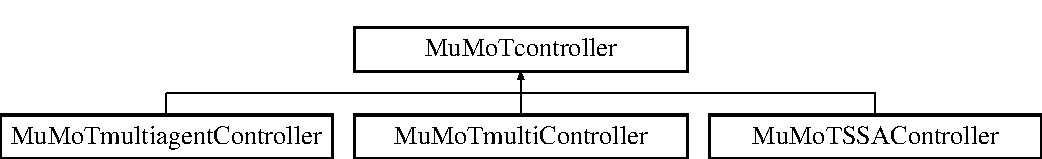
\includegraphics[height=2.000000cm]{class_mu_mo_t_1_1_mu_mo_t_1_1_mu_mo_tcontroller}
\end{center}
\end{figure}
\subsection*{Public Member Functions}
\begin{DoxyCompactItemize}
\item 
def \hyperlink{class_mu_mo_t_1_1_mu_mo_t_1_1_mu_mo_tcontroller_a2b7e9681302740635162f2f8f0dddebf}{\+\_\+\+\_\+init\+\_\+\+\_\+} (self, param\+Values, param\+Names, param\+Label\+Dict=\{\}, continuous\+Replot=\hyperlink{namespace_mu_mo_t_1_1_mu_mo_t_a36cde68b055f3f2ee671020af4ccf4e2}{False}, plot\+Limits=\hyperlink{namespace_mu_mo_t_1_1_mu_mo_t_a36cde68b055f3f2ee671020af4ccf4e2}{False}, system\+Size=\hyperlink{namespace_mu_mo_t_1_1_mu_mo_t_a36cde68b055f3f2ee671020af4ccf4e2}{False}, params=None, kwargs)
\end{DoxyCompactItemize}
\subsection*{Static Public Attributes}
\begin{DoxyCompactItemize}
\item 
\hyperlink{class_mu_mo_t_1_1_mu_mo_t_1_1_mu_mo_tcontroller_a7018be3799b9e7cec083030398c0530f}{fixed\+Params}
\item 
\hyperlink{class_mu_mo_t_1_1_mu_mo_t_1_1_mu_mo_tcontroller_afdba98970961edb29f88241b9d99d890}{foo}
\item 
list \hyperlink{class_mu_mo_t_1_1_mu_mo_t_1_1_mu_mo_tcontroller_a8ae52d3e73fa16e877bf17d4af74c80d}{fixed\+Params\+Decoded} = \mbox{[}$\,$\mbox{]}
\item 
\hyperlink{class_mu_mo_t_1_1_mu_mo_t_1_1_mu_mo_tcontroller_a0358810928b8858d2b7cbfc344ba792a}{expr} = process\+\_\+sympy(fixed\+Param.\+replace(\textquotesingle{}\textbackslash{}\textbackslash{}\textbackslash{}\textbackslash{}\textquotesingle{},\textquotesingle{}\textbackslash{}\textbackslash{}\textquotesingle{}))
\item 
\hyperlink{class_mu_mo_t_1_1_mu_mo_t_1_1_mu_mo_tcontroller_a1e15bdfe806c9eac0e6af33fa402bdde}{atoms} = expr.\+atoms()
\end{DoxyCompactItemize}
\subsection*{Private Attributes}
\begin{DoxyCompactItemize}
\item 
\hyperlink{class_mu_mo_t_1_1_mu_mo_t_1_1_mu_mo_tcontroller_a909146a3c119c927727c7d533042b184}{\+\_\+silent}
\end{DoxyCompactItemize}
\subsection*{Static Private Attributes}
\begin{DoxyCompactItemize}
\item 
\hyperlink{class_mu_mo_t_1_1_mu_mo_t_1_1_mu_mo_tcontroller_a27dd8543b5188cdfe40f622d267fe2c5}{\+\_\+view} = None
\item 
\hyperlink{class_mu_mo_t_1_1_mu_mo_t_1_1_mu_mo_tcontroller_a13bcda33e0e971cf4ad2710945226add}{\+\_\+param\+Label\+Dict} = None
\begin{DoxyCompactList}\small\item\em dictionary of La\+TeX labels for widgets, with parameter name as key \end{DoxyCompactList}\item 
\hyperlink{class_mu_mo_t_1_1_mu_mo_t_1_1_mu_mo_tcontroller_aab884266838b2bf42f4ff27cc2041464}{\+\_\+widgets\+Free\+Params} = None
\begin{DoxyCompactList}\small\item\em dictionary of controller widgets only for the free parameters of the model, with parameter name as key \end{DoxyCompactList}\item 
\hyperlink{class_mu_mo_t_1_1_mu_mo_t_1_1_mu_mo_tcontroller_aae2fc2e1d31d0fd22ea078bb930222a4}{\+\_\+widgets\+Extra\+Params} = None
\begin{DoxyCompactList}\small\item\em dictionary of controller widgets for the special parameters (e.\+g., simulation length, initial state), with parameter name as key \end{DoxyCompactList}\item 
\hyperlink{class_mu_mo_t_1_1_mu_mo_t_1_1_mu_mo_tcontroller_af54e883f58d2be155299935e0bf427cb}{\+\_\+widgets\+Plot\+Only} = None
\begin{DoxyCompactList}\small\item\em dictionary of controller widgets, with parameter that influence only the plotting and not the computation \end{DoxyCompactList}\item 
\hyperlink{class_mu_mo_t_1_1_mu_mo_t_1_1_mu_mo_tcontroller_a04e66f2b7e3c67b0e96f318acbfa7f0e}{\+\_\+replot\+Function} = None
\begin{DoxyCompactList}\small\item\em replot function widgets have been assigned (for use by \hyperlink{class_mu_mo_t_1_1_mu_mo_t_1_1_mu_mo_tmulti_controller}{Mu\+Mo\+Tmulti\+Controller}) \end{DoxyCompactList}\item 
\hyperlink{class_mu_mo_t_1_1_mu_mo_t_1_1_mu_mo_tcontroller_afb9cc1f1f0c08393b454f526842425cc}{\+\_\+error\+Message} = None
\begin{DoxyCompactList}\small\item\em widget for simple error messages to be displayed to user during interaction \end{DoxyCompactList}\item 
\hyperlink{class_mu_mo_t_1_1_mu_mo_t_1_1_mu_mo_tcontroller_a7f7ea1e7e5688cb25a6651783db498e0}{\+\_\+plot\+Limits\+Widget} = None
\begin{DoxyCompactList}\small\item\em plot limits slider widget \end{DoxyCompactList}\item 
\hyperlink{class_mu_mo_t_1_1_mu_mo_t_1_1_mu_mo_tcontroller_ab1e13c5ff312caa1398f9de296be2319}{\+\_\+system\+Size\+Widget} = None
\begin{DoxyCompactList}\small\item\em system size slider widget \end{DoxyCompactList}\item 
\hyperlink{class_mu_mo_t_1_1_mu_mo_t_1_1_mu_mo_tcontroller_ae7a084d9f77bbda4a99577633ef002ce}{\+\_\+bookmark\+Widget} = None
\begin{DoxyCompactList}\small\item\em bookmark button widget \end{DoxyCompactList}\item 
\hyperlink{class_mu_mo_t_1_1_mu_mo_t_1_1_mu_mo_tcontroller_a018864aa22d2adb0d3958fb0adbce8e2}{\+\_\+progress\+Bar} = None
\begin{DoxyCompactList}\small\item\em progress bar \end{DoxyCompactList}\item 
\hyperlink{class_mu_mo_t_1_1_mu_mo_t_1_1_mu_mo_tcontroller_a1da52cde6b2b94a1005eaa6898d2f8c5}{\+\_\+progress\+Bar\+\_\+multi} = None
\begin{DoxyCompactList}\small\item\em used two progress bars, otherwise the previous cell bar (where controller is created) does not react anymore \end{DoxyCompactList}\end{DoxyCompactItemize}


\subsection{Detailed Description}
class describing a controller for a model view 

\subsection{Constructor \& Destructor Documentation}
\mbox{\Hypertarget{class_mu_mo_t_1_1_mu_mo_t_1_1_mu_mo_tcontroller_a2b7e9681302740635162f2f8f0dddebf}\label{class_mu_mo_t_1_1_mu_mo_t_1_1_mu_mo_tcontroller_a2b7e9681302740635162f2f8f0dddebf}} 
\index{Mu\+Mo\+T\+::\+Mu\+Mo\+T\+::\+Mu\+Mo\+Tcontroller@{Mu\+Mo\+T\+::\+Mu\+Mo\+T\+::\+Mu\+Mo\+Tcontroller}!\+\_\+\+\_\+init\+\_\+\+\_\+@{\+\_\+\+\_\+init\+\_\+\+\_\+}}
\index{\+\_\+\+\_\+init\+\_\+\+\_\+@{\+\_\+\+\_\+init\+\_\+\+\_\+}!Mu\+Mo\+T\+::\+Mu\+Mo\+T\+::\+Mu\+Mo\+Tcontroller@{Mu\+Mo\+T\+::\+Mu\+Mo\+T\+::\+Mu\+Mo\+Tcontroller}}
\subsubsection{\texorpdfstring{\+\_\+\+\_\+init\+\_\+\+\_\+()}{\_\_init\_\_()}}
{\footnotesize\ttfamily def \+\_\+\+\_\+init\+\_\+\+\_\+ (\begin{DoxyParamCaption}\item[{}]{self,  }\item[{}]{param\+Values,  }\item[{}]{param\+Names,  }\item[{}]{param\+Label\+Dict = {\ttfamily \{\}},  }\item[{}]{continuous\+Replot = {\ttfamily \hyperlink{namespace_mu_mo_t_1_1_mu_mo_t_a36cde68b055f3f2ee671020af4ccf4e2}{False}},  }\item[{}]{plot\+Limits = {\ttfamily \hyperlink{namespace_mu_mo_t_1_1_mu_mo_t_a36cde68b055f3f2ee671020af4ccf4e2}{False}},  }\item[{}]{system\+Size = {\ttfamily \hyperlink{namespace_mu_mo_t_1_1_mu_mo_t_a36cde68b055f3f2ee671020af4ccf4e2}{False}},  }\item[{}]{params = {\ttfamily None},  }\item[{}]{kwargs }\end{DoxyParamCaption})}



\subsection{Field Documentation}
\mbox{\Hypertarget{class_mu_mo_t_1_1_mu_mo_t_1_1_mu_mo_tcontroller_ae7a084d9f77bbda4a99577633ef002ce}\label{class_mu_mo_t_1_1_mu_mo_t_1_1_mu_mo_tcontroller_ae7a084d9f77bbda4a99577633ef002ce}} 
\index{Mu\+Mo\+T\+::\+Mu\+Mo\+T\+::\+Mu\+Mo\+Tcontroller@{Mu\+Mo\+T\+::\+Mu\+Mo\+T\+::\+Mu\+Mo\+Tcontroller}!\+\_\+bookmark\+Widget@{\+\_\+bookmark\+Widget}}
\index{\+\_\+bookmark\+Widget@{\+\_\+bookmark\+Widget}!Mu\+Mo\+T\+::\+Mu\+Mo\+T\+::\+Mu\+Mo\+Tcontroller@{Mu\+Mo\+T\+::\+Mu\+Mo\+T\+::\+Mu\+Mo\+Tcontroller}}
\subsubsection{\texorpdfstring{\+\_\+bookmark\+Widget}{\_bookmarkWidget}}
{\footnotesize\ttfamily \+\_\+bookmark\+Widget = None\hspace{0.3cm}{\ttfamily [static]}, {\ttfamily [private]}}



bookmark button widget 

\mbox{\Hypertarget{class_mu_mo_t_1_1_mu_mo_t_1_1_mu_mo_tcontroller_afb9cc1f1f0c08393b454f526842425cc}\label{class_mu_mo_t_1_1_mu_mo_t_1_1_mu_mo_tcontroller_afb9cc1f1f0c08393b454f526842425cc}} 
\index{Mu\+Mo\+T\+::\+Mu\+Mo\+T\+::\+Mu\+Mo\+Tcontroller@{Mu\+Mo\+T\+::\+Mu\+Mo\+T\+::\+Mu\+Mo\+Tcontroller}!\+\_\+error\+Message@{\+\_\+error\+Message}}
\index{\+\_\+error\+Message@{\+\_\+error\+Message}!Mu\+Mo\+T\+::\+Mu\+Mo\+T\+::\+Mu\+Mo\+Tcontroller@{Mu\+Mo\+T\+::\+Mu\+Mo\+T\+::\+Mu\+Mo\+Tcontroller}}
\subsubsection{\texorpdfstring{\+\_\+error\+Message}{\_errorMessage}}
{\footnotesize\ttfamily \+\_\+error\+Message = None\hspace{0.3cm}{\ttfamily [static]}, {\ttfamily [private]}}



widget for simple error messages to be displayed to user during interaction 

\mbox{\Hypertarget{class_mu_mo_t_1_1_mu_mo_t_1_1_mu_mo_tcontroller_a13bcda33e0e971cf4ad2710945226add}\label{class_mu_mo_t_1_1_mu_mo_t_1_1_mu_mo_tcontroller_a13bcda33e0e971cf4ad2710945226add}} 
\index{Mu\+Mo\+T\+::\+Mu\+Mo\+T\+::\+Mu\+Mo\+Tcontroller@{Mu\+Mo\+T\+::\+Mu\+Mo\+T\+::\+Mu\+Mo\+Tcontroller}!\+\_\+param\+Label\+Dict@{\+\_\+param\+Label\+Dict}}
\index{\+\_\+param\+Label\+Dict@{\+\_\+param\+Label\+Dict}!Mu\+Mo\+T\+::\+Mu\+Mo\+T\+::\+Mu\+Mo\+Tcontroller@{Mu\+Mo\+T\+::\+Mu\+Mo\+T\+::\+Mu\+Mo\+Tcontroller}}
\subsubsection{\texorpdfstring{\+\_\+param\+Label\+Dict}{\_paramLabelDict}}
{\footnotesize\ttfamily \+\_\+param\+Label\+Dict = None\hspace{0.3cm}{\ttfamily [static]}, {\ttfamily [private]}}



dictionary of La\+TeX labels for widgets, with parameter name as key 

\mbox{\Hypertarget{class_mu_mo_t_1_1_mu_mo_t_1_1_mu_mo_tcontroller_a7f7ea1e7e5688cb25a6651783db498e0}\label{class_mu_mo_t_1_1_mu_mo_t_1_1_mu_mo_tcontroller_a7f7ea1e7e5688cb25a6651783db498e0}} 
\index{Mu\+Mo\+T\+::\+Mu\+Mo\+T\+::\+Mu\+Mo\+Tcontroller@{Mu\+Mo\+T\+::\+Mu\+Mo\+T\+::\+Mu\+Mo\+Tcontroller}!\+\_\+plot\+Limits\+Widget@{\+\_\+plot\+Limits\+Widget}}
\index{\+\_\+plot\+Limits\+Widget@{\+\_\+plot\+Limits\+Widget}!Mu\+Mo\+T\+::\+Mu\+Mo\+T\+::\+Mu\+Mo\+Tcontroller@{Mu\+Mo\+T\+::\+Mu\+Mo\+T\+::\+Mu\+Mo\+Tcontroller}}
\subsubsection{\texorpdfstring{\+\_\+plot\+Limits\+Widget}{\_plotLimitsWidget}}
{\footnotesize\ttfamily \+\_\+plot\+Limits\+Widget = None\hspace{0.3cm}{\ttfamily [static]}, {\ttfamily [private]}}



plot limits slider widget 

\mbox{\Hypertarget{class_mu_mo_t_1_1_mu_mo_t_1_1_mu_mo_tcontroller_a018864aa22d2adb0d3958fb0adbce8e2}\label{class_mu_mo_t_1_1_mu_mo_t_1_1_mu_mo_tcontroller_a018864aa22d2adb0d3958fb0adbce8e2}} 
\index{Mu\+Mo\+T\+::\+Mu\+Mo\+T\+::\+Mu\+Mo\+Tcontroller@{Mu\+Mo\+T\+::\+Mu\+Mo\+T\+::\+Mu\+Mo\+Tcontroller}!\+\_\+progress\+Bar@{\+\_\+progress\+Bar}}
\index{\+\_\+progress\+Bar@{\+\_\+progress\+Bar}!Mu\+Mo\+T\+::\+Mu\+Mo\+T\+::\+Mu\+Mo\+Tcontroller@{Mu\+Mo\+T\+::\+Mu\+Mo\+T\+::\+Mu\+Mo\+Tcontroller}}
\subsubsection{\texorpdfstring{\+\_\+progress\+Bar}{\_progressBar}}
{\footnotesize\ttfamily \+\_\+progress\+Bar = None\hspace{0.3cm}{\ttfamily [static]}, {\ttfamily [private]}}



progress bar 

\begin{DoxyRefDesc}{Todo}
\item[\hyperlink{todo__todo000023}{Todo}]\+: is this best put in base class when it is not always used? \end{DoxyRefDesc}
\mbox{\Hypertarget{class_mu_mo_t_1_1_mu_mo_t_1_1_mu_mo_tcontroller_a1da52cde6b2b94a1005eaa6898d2f8c5}\label{class_mu_mo_t_1_1_mu_mo_t_1_1_mu_mo_tcontroller_a1da52cde6b2b94a1005eaa6898d2f8c5}} 
\index{Mu\+Mo\+T\+::\+Mu\+Mo\+T\+::\+Mu\+Mo\+Tcontroller@{Mu\+Mo\+T\+::\+Mu\+Mo\+T\+::\+Mu\+Mo\+Tcontroller}!\+\_\+progress\+Bar\+\_\+multi@{\+\_\+progress\+Bar\+\_\+multi}}
\index{\+\_\+progress\+Bar\+\_\+multi@{\+\_\+progress\+Bar\+\_\+multi}!Mu\+Mo\+T\+::\+Mu\+Mo\+T\+::\+Mu\+Mo\+Tcontroller@{Mu\+Mo\+T\+::\+Mu\+Mo\+T\+::\+Mu\+Mo\+Tcontroller}}
\subsubsection{\texorpdfstring{\+\_\+progress\+Bar\+\_\+multi}{\_progressBar\_multi}}
{\footnotesize\ttfamily \+\_\+progress\+Bar\+\_\+multi = None\hspace{0.3cm}{\ttfamily [static]}, {\ttfamily [private]}}



used two progress bars, otherwise the previous cell bar (where controller is created) does not react anymore 

\begin{DoxyRefDesc}{Todo}
\item[\hyperlink{todo__todo000024}{Todo}]\+: is this best put in base class when it is not always used? \end{DoxyRefDesc}
\mbox{\Hypertarget{class_mu_mo_t_1_1_mu_mo_t_1_1_mu_mo_tcontroller_a04e66f2b7e3c67b0e96f318acbfa7f0e}\label{class_mu_mo_t_1_1_mu_mo_t_1_1_mu_mo_tcontroller_a04e66f2b7e3c67b0e96f318acbfa7f0e}} 
\index{Mu\+Mo\+T\+::\+Mu\+Mo\+T\+::\+Mu\+Mo\+Tcontroller@{Mu\+Mo\+T\+::\+Mu\+Mo\+T\+::\+Mu\+Mo\+Tcontroller}!\+\_\+replot\+Function@{\+\_\+replot\+Function}}
\index{\+\_\+replot\+Function@{\+\_\+replot\+Function}!Mu\+Mo\+T\+::\+Mu\+Mo\+T\+::\+Mu\+Mo\+Tcontroller@{Mu\+Mo\+T\+::\+Mu\+Mo\+T\+::\+Mu\+Mo\+Tcontroller}}
\subsubsection{\texorpdfstring{\+\_\+replot\+Function}{\_replotFunction}}
{\footnotesize\ttfamily \+\_\+replot\+Function = None\hspace{0.3cm}{\ttfamily [static]}, {\ttfamily [private]}}



replot function widgets have been assigned (for use by \hyperlink{class_mu_mo_t_1_1_mu_mo_t_1_1_mu_mo_tmulti_controller}{Mu\+Mo\+Tmulti\+Controller}) 

\mbox{\Hypertarget{class_mu_mo_t_1_1_mu_mo_t_1_1_mu_mo_tcontroller_a909146a3c119c927727c7d533042b184}\label{class_mu_mo_t_1_1_mu_mo_t_1_1_mu_mo_tcontroller_a909146a3c119c927727c7d533042b184}} 
\index{Mu\+Mo\+T\+::\+Mu\+Mo\+T\+::\+Mu\+Mo\+Tcontroller@{Mu\+Mo\+T\+::\+Mu\+Mo\+T\+::\+Mu\+Mo\+Tcontroller}!\+\_\+silent@{\+\_\+silent}}
\index{\+\_\+silent@{\+\_\+silent}!Mu\+Mo\+T\+::\+Mu\+Mo\+T\+::\+Mu\+Mo\+Tcontroller@{Mu\+Mo\+T\+::\+Mu\+Mo\+T\+::\+Mu\+Mo\+Tcontroller}}
\subsubsection{\texorpdfstring{\+\_\+silent}{\_silent}}
{\footnotesize\ttfamily \+\_\+silent\hspace{0.3cm}{\ttfamily [private]}}

\mbox{\Hypertarget{class_mu_mo_t_1_1_mu_mo_t_1_1_mu_mo_tcontroller_ab1e13c5ff312caa1398f9de296be2319}\label{class_mu_mo_t_1_1_mu_mo_t_1_1_mu_mo_tcontroller_ab1e13c5ff312caa1398f9de296be2319}} 
\index{Mu\+Mo\+T\+::\+Mu\+Mo\+T\+::\+Mu\+Mo\+Tcontroller@{Mu\+Mo\+T\+::\+Mu\+Mo\+T\+::\+Mu\+Mo\+Tcontroller}!\+\_\+system\+Size\+Widget@{\+\_\+system\+Size\+Widget}}
\index{\+\_\+system\+Size\+Widget@{\+\_\+system\+Size\+Widget}!Mu\+Mo\+T\+::\+Mu\+Mo\+T\+::\+Mu\+Mo\+Tcontroller@{Mu\+Mo\+T\+::\+Mu\+Mo\+T\+::\+Mu\+Mo\+Tcontroller}}
\subsubsection{\texorpdfstring{\+\_\+system\+Size\+Widget}{\_systemSizeWidget}}
{\footnotesize\ttfamily \+\_\+system\+Size\+Widget = None\hspace{0.3cm}{\ttfamily [static]}, {\ttfamily [private]}}



system size slider widget 

\mbox{\Hypertarget{class_mu_mo_t_1_1_mu_mo_t_1_1_mu_mo_tcontroller_a27dd8543b5188cdfe40f622d267fe2c5}\label{class_mu_mo_t_1_1_mu_mo_t_1_1_mu_mo_tcontroller_a27dd8543b5188cdfe40f622d267fe2c5}} 
\index{Mu\+Mo\+T\+::\+Mu\+Mo\+T\+::\+Mu\+Mo\+Tcontroller@{Mu\+Mo\+T\+::\+Mu\+Mo\+T\+::\+Mu\+Mo\+Tcontroller}!\+\_\+view@{\+\_\+view}}
\index{\+\_\+view@{\+\_\+view}!Mu\+Mo\+T\+::\+Mu\+Mo\+T\+::\+Mu\+Mo\+Tcontroller@{Mu\+Mo\+T\+::\+Mu\+Mo\+T\+::\+Mu\+Mo\+Tcontroller}}
\subsubsection{\texorpdfstring{\+\_\+view}{\_view}}
{\footnotesize\ttfamily \+\_\+view = None\hspace{0.3cm}{\ttfamily [static]}, {\ttfamily [private]}}

\mbox{\Hypertarget{class_mu_mo_t_1_1_mu_mo_t_1_1_mu_mo_tcontroller_aae2fc2e1d31d0fd22ea078bb930222a4}\label{class_mu_mo_t_1_1_mu_mo_t_1_1_mu_mo_tcontroller_aae2fc2e1d31d0fd22ea078bb930222a4}} 
\index{Mu\+Mo\+T\+::\+Mu\+Mo\+T\+::\+Mu\+Mo\+Tcontroller@{Mu\+Mo\+T\+::\+Mu\+Mo\+T\+::\+Mu\+Mo\+Tcontroller}!\+\_\+widgets\+Extra\+Params@{\+\_\+widgets\+Extra\+Params}}
\index{\+\_\+widgets\+Extra\+Params@{\+\_\+widgets\+Extra\+Params}!Mu\+Mo\+T\+::\+Mu\+Mo\+T\+::\+Mu\+Mo\+Tcontroller@{Mu\+Mo\+T\+::\+Mu\+Mo\+T\+::\+Mu\+Mo\+Tcontroller}}
\subsubsection{\texorpdfstring{\+\_\+widgets\+Extra\+Params}{\_widgetsExtraParams}}
{\footnotesize\ttfamily \+\_\+widgets\+Extra\+Params = None\hspace{0.3cm}{\ttfamily [static]}, {\ttfamily [private]}}



dictionary of controller widgets for the special parameters (e.\+g., simulation length, initial state), with parameter name as key 

\mbox{\Hypertarget{class_mu_mo_t_1_1_mu_mo_t_1_1_mu_mo_tcontroller_aab884266838b2bf42f4ff27cc2041464}\label{class_mu_mo_t_1_1_mu_mo_t_1_1_mu_mo_tcontroller_aab884266838b2bf42f4ff27cc2041464}} 
\index{Mu\+Mo\+T\+::\+Mu\+Mo\+T\+::\+Mu\+Mo\+Tcontroller@{Mu\+Mo\+T\+::\+Mu\+Mo\+T\+::\+Mu\+Mo\+Tcontroller}!\+\_\+widgets\+Free\+Params@{\+\_\+widgets\+Free\+Params}}
\index{\+\_\+widgets\+Free\+Params@{\+\_\+widgets\+Free\+Params}!Mu\+Mo\+T\+::\+Mu\+Mo\+T\+::\+Mu\+Mo\+Tcontroller@{Mu\+Mo\+T\+::\+Mu\+Mo\+T\+::\+Mu\+Mo\+Tcontroller}}
\subsubsection{\texorpdfstring{\+\_\+widgets\+Free\+Params}{\_widgetsFreeParams}}
{\footnotesize\ttfamily \+\_\+widgets\+Free\+Params = None\hspace{0.3cm}{\ttfamily [static]}, {\ttfamily [private]}}



dictionary of controller widgets only for the free parameters of the model, with parameter name as key 

\mbox{\Hypertarget{class_mu_mo_t_1_1_mu_mo_t_1_1_mu_mo_tcontroller_af54e883f58d2be155299935e0bf427cb}\label{class_mu_mo_t_1_1_mu_mo_t_1_1_mu_mo_tcontroller_af54e883f58d2be155299935e0bf427cb}} 
\index{Mu\+Mo\+T\+::\+Mu\+Mo\+T\+::\+Mu\+Mo\+Tcontroller@{Mu\+Mo\+T\+::\+Mu\+Mo\+T\+::\+Mu\+Mo\+Tcontroller}!\+\_\+widgets\+Plot\+Only@{\+\_\+widgets\+Plot\+Only}}
\index{\+\_\+widgets\+Plot\+Only@{\+\_\+widgets\+Plot\+Only}!Mu\+Mo\+T\+::\+Mu\+Mo\+T\+::\+Mu\+Mo\+Tcontroller@{Mu\+Mo\+T\+::\+Mu\+Mo\+T\+::\+Mu\+Mo\+Tcontroller}}
\subsubsection{\texorpdfstring{\+\_\+widgets\+Plot\+Only}{\_widgetsPlotOnly}}
{\footnotesize\ttfamily \+\_\+widgets\+Plot\+Only = None\hspace{0.3cm}{\ttfamily [static]}, {\ttfamily [private]}}



dictionary of controller widgets, with parameter that influence only the plotting and not the computation 

\mbox{\Hypertarget{class_mu_mo_t_1_1_mu_mo_t_1_1_mu_mo_tcontroller_a1e15bdfe806c9eac0e6af33fa402bdde}\label{class_mu_mo_t_1_1_mu_mo_t_1_1_mu_mo_tcontroller_a1e15bdfe806c9eac0e6af33fa402bdde}} 
\index{Mu\+Mo\+T\+::\+Mu\+Mo\+T\+::\+Mu\+Mo\+Tcontroller@{Mu\+Mo\+T\+::\+Mu\+Mo\+T\+::\+Mu\+Mo\+Tcontroller}!atoms@{atoms}}
\index{atoms@{atoms}!Mu\+Mo\+T\+::\+Mu\+Mo\+T\+::\+Mu\+Mo\+Tcontroller@{Mu\+Mo\+T\+::\+Mu\+Mo\+T\+::\+Mu\+Mo\+Tcontroller}}
\subsubsection{\texorpdfstring{atoms}{atoms}}
{\footnotesize\ttfamily atoms = expr.\+atoms()\hspace{0.3cm}{\ttfamily [static]}}

\mbox{\Hypertarget{class_mu_mo_t_1_1_mu_mo_t_1_1_mu_mo_tcontroller_a0358810928b8858d2b7cbfc344ba792a}\label{class_mu_mo_t_1_1_mu_mo_t_1_1_mu_mo_tcontroller_a0358810928b8858d2b7cbfc344ba792a}} 
\index{Mu\+Mo\+T\+::\+Mu\+Mo\+T\+::\+Mu\+Mo\+Tcontroller@{Mu\+Mo\+T\+::\+Mu\+Mo\+T\+::\+Mu\+Mo\+Tcontroller}!expr@{expr}}
\index{expr@{expr}!Mu\+Mo\+T\+::\+Mu\+Mo\+T\+::\+Mu\+Mo\+Tcontroller@{Mu\+Mo\+T\+::\+Mu\+Mo\+T\+::\+Mu\+Mo\+Tcontroller}}
\subsubsection{\texorpdfstring{expr}{expr}}
{\footnotesize\ttfamily expr = process\+\_\+sympy(fixed\+Param.\+replace(\textquotesingle{}\textbackslash{}\textbackslash{}\textbackslash{}\textbackslash{}\textquotesingle{},\textquotesingle{}\textbackslash{}\textbackslash{}\textquotesingle{}))\hspace{0.3cm}{\ttfamily [static]}}

\mbox{\Hypertarget{class_mu_mo_t_1_1_mu_mo_t_1_1_mu_mo_tcontroller_a7018be3799b9e7cec083030398c0530f}\label{class_mu_mo_t_1_1_mu_mo_t_1_1_mu_mo_tcontroller_a7018be3799b9e7cec083030398c0530f}} 
\index{Mu\+Mo\+T\+::\+Mu\+Mo\+T\+::\+Mu\+Mo\+Tcontroller@{Mu\+Mo\+T\+::\+Mu\+Mo\+T\+::\+Mu\+Mo\+Tcontroller}!fixed\+Params@{fixed\+Params}}
\index{fixed\+Params@{fixed\+Params}!Mu\+Mo\+T\+::\+Mu\+Mo\+T\+::\+Mu\+Mo\+Tcontroller@{Mu\+Mo\+T\+::\+Mu\+Mo\+T\+::\+Mu\+Mo\+Tcontroller}}
\subsubsection{\texorpdfstring{fixed\+Params}{fixedParams}}
{\footnotesize\ttfamily fixed\+Params\hspace{0.3cm}{\ttfamily [static]}}

\mbox{\Hypertarget{class_mu_mo_t_1_1_mu_mo_t_1_1_mu_mo_tcontroller_a8ae52d3e73fa16e877bf17d4af74c80d}\label{class_mu_mo_t_1_1_mu_mo_t_1_1_mu_mo_tcontroller_a8ae52d3e73fa16e877bf17d4af74c80d}} 
\index{Mu\+Mo\+T\+::\+Mu\+Mo\+T\+::\+Mu\+Mo\+Tcontroller@{Mu\+Mo\+T\+::\+Mu\+Mo\+T\+::\+Mu\+Mo\+Tcontroller}!fixed\+Params\+Decoded@{fixed\+Params\+Decoded}}
\index{fixed\+Params\+Decoded@{fixed\+Params\+Decoded}!Mu\+Mo\+T\+::\+Mu\+Mo\+T\+::\+Mu\+Mo\+Tcontroller@{Mu\+Mo\+T\+::\+Mu\+Mo\+T\+::\+Mu\+Mo\+Tcontroller}}
\subsubsection{\texorpdfstring{fixed\+Params\+Decoded}{fixedParamsDecoded}}
{\footnotesize\ttfamily list fixed\+Params\+Decoded = \mbox{[}$\,$\mbox{]}\hspace{0.3cm}{\ttfamily [static]}}

\mbox{\Hypertarget{class_mu_mo_t_1_1_mu_mo_t_1_1_mu_mo_tcontroller_afdba98970961edb29f88241b9d99d890}\label{class_mu_mo_t_1_1_mu_mo_t_1_1_mu_mo_tcontroller_afdba98970961edb29f88241b9d99d890}} 
\index{Mu\+Mo\+T\+::\+Mu\+Mo\+T\+::\+Mu\+Mo\+Tcontroller@{Mu\+Mo\+T\+::\+Mu\+Mo\+T\+::\+Mu\+Mo\+Tcontroller}!foo@{foo}}
\index{foo@{foo}!Mu\+Mo\+T\+::\+Mu\+Mo\+T\+::\+Mu\+Mo\+Tcontroller@{Mu\+Mo\+T\+::\+Mu\+Mo\+T\+::\+Mu\+Mo\+Tcontroller}}
\subsubsection{\texorpdfstring{foo}{foo}}
{\footnotesize\ttfamily foo\hspace{0.3cm}{\ttfamily [static]}}



The documentation for this class was generated from the following file\+:\begin{DoxyCompactItemize}
\item 
Mu\+Mo\+T/\hyperlink{_mu_mo_t_8py}{Mu\+Mo\+T.\+py}\end{DoxyCompactItemize}

\hypertarget{class_mu_mo_t_1_1_mu_mo_t_1_1_mu_mo_tdefault}{}\section{Mu\+Mo\+Tdefault Class Reference}
\label{class_mu_mo_t_1_1_mu_mo_t_1_1_mu_mo_tdefault}\index{Mu\+Mo\+Tdefault@{Mu\+Mo\+Tdefault}}
\subsection*{Static Public Member Functions}
\begin{DoxyCompactItemize}
\item 
def \hyperlink{class_mu_mo_t_1_1_mu_mo_t_1_1_mu_mo_tdefault_a3ce665e68925e7c173896a5101b16dfa}{set\+Rate\+Defaults} (init\+Rate=\hyperlink{class_mu_mo_t_1_1_mu_mo_t_1_1_mu_mo_tdefault_adbfda01292fc4c7936ed57523fd625c7}{\+\_\+initial\+Rate\+Value}, limits=\hyperlink{class_mu_mo_t_1_1_mu_mo_t_1_1_mu_mo_tdefault_a89f788e3d778e1e0554c57832275d484}{\+\_\+rate\+Limits}, step=\hyperlink{class_mu_mo_t_1_1_mu_mo_t_1_1_mu_mo_tdefault_aa45ec6be070d9881c9c018a533f6573c}{\+\_\+rate\+Step})
\item 
def \hyperlink{class_mu_mo_t_1_1_mu_mo_t_1_1_mu_mo_tdefault_a4be4721ce31fd644cb66ae8af0dd41fe}{set\+Time\+Defaults} (init\+Time=\hyperlink{class_mu_mo_t_1_1_mu_mo_t_1_1_mu_mo_tdefault_a46ffe9aa10cdab976a57d8ba1d3cd2f6}{\+\_\+max\+Time}, limits=\hyperlink{class_mu_mo_t_1_1_mu_mo_t_1_1_mu_mo_tdefault_a2208809031da7f126f4416fb64cdb026}{\+\_\+time\+Limits}, step=\hyperlink{class_mu_mo_t_1_1_mu_mo_t_1_1_mu_mo_tdefault_ad83203bcc6032b30e6f5b57f8982af9e}{\+\_\+time\+Step})
\item 
def \hyperlink{class_mu_mo_t_1_1_mu_mo_t_1_1_mu_mo_tdefault_a390063ec9e63f433bf06fa72f608b7e4}{set\+Agents\+Defaults} (init\+Agents=\hyperlink{class_mu_mo_t_1_1_mu_mo_t_1_1_mu_mo_tdefault_a42f05ec35f2b5b564e064bb19ebd36cf}{\+\_\+agents}, limits=\hyperlink{class_mu_mo_t_1_1_mu_mo_t_1_1_mu_mo_tdefault_a01360abcb6eddb212c38b66852c35e17}{\+\_\+agents\+Limits}, step=\hyperlink{class_mu_mo_t_1_1_mu_mo_t_1_1_mu_mo_tdefault_a55b7c54066a90600796a35e96ef5743b}{\+\_\+agents\+Step})
\end{DoxyCompactItemize}
\subsection*{Static Private Attributes}
\begin{DoxyCompactItemize}
\item 
int \hyperlink{class_mu_mo_t_1_1_mu_mo_t_1_1_mu_mo_tdefault_adbfda01292fc4c7936ed57523fd625c7}{\+\_\+initial\+Rate\+Value} = 2
\item 
tuple \hyperlink{class_mu_mo_t_1_1_mu_mo_t_1_1_mu_mo_tdefault_a89f788e3d778e1e0554c57832275d484}{\+\_\+rate\+Limits} = (0.\+0, 20.\+0)
\item 
float \hyperlink{class_mu_mo_t_1_1_mu_mo_t_1_1_mu_mo_tdefault_aa45ec6be070d9881c9c018a533f6573c}{\+\_\+rate\+Step} = 0.\+1
\item 
int \hyperlink{class_mu_mo_t_1_1_mu_mo_t_1_1_mu_mo_tdefault_a46ffe9aa10cdab976a57d8ba1d3cd2f6}{\+\_\+max\+Time} = 10
\item 
tuple \hyperlink{class_mu_mo_t_1_1_mu_mo_t_1_1_mu_mo_tdefault_a2208809031da7f126f4416fb64cdb026}{\+\_\+time\+Limits} = (1, 100)
\item 
int \hyperlink{class_mu_mo_t_1_1_mu_mo_t_1_1_mu_mo_tdefault_ad83203bcc6032b30e6f5b57f8982af9e}{\+\_\+time\+Step} = 1
\item 
int \hyperlink{class_mu_mo_t_1_1_mu_mo_t_1_1_mu_mo_tdefault_a42f05ec35f2b5b564e064bb19ebd36cf}{\+\_\+agents} = 100
\item 
tuple \hyperlink{class_mu_mo_t_1_1_mu_mo_t_1_1_mu_mo_tdefault_a01360abcb6eddb212c38b66852c35e17}{\+\_\+agents\+Limits} = (0, 1000)
\item 
int \hyperlink{class_mu_mo_t_1_1_mu_mo_t_1_1_mu_mo_tdefault_a55b7c54066a90600796a35e96ef5743b}{\+\_\+agents\+Step} = 1
\end{DoxyCompactItemize}


\subsection{Member Function Documentation}
\mbox{\Hypertarget{class_mu_mo_t_1_1_mu_mo_t_1_1_mu_mo_tdefault_a390063ec9e63f433bf06fa72f608b7e4}\label{class_mu_mo_t_1_1_mu_mo_t_1_1_mu_mo_tdefault_a390063ec9e63f433bf06fa72f608b7e4}} 
\index{Mu\+Mo\+T\+::\+Mu\+Mo\+T\+::\+Mu\+Mo\+Tdefault@{Mu\+Mo\+T\+::\+Mu\+Mo\+T\+::\+Mu\+Mo\+Tdefault}!set\+Agents\+Defaults@{set\+Agents\+Defaults}}
\index{set\+Agents\+Defaults@{set\+Agents\+Defaults}!Mu\+Mo\+T\+::\+Mu\+Mo\+T\+::\+Mu\+Mo\+Tdefault@{Mu\+Mo\+T\+::\+Mu\+Mo\+T\+::\+Mu\+Mo\+Tdefault}}
\subsubsection{\texorpdfstring{set\+Agents\+Defaults()}{setAgentsDefaults()}}
{\footnotesize\ttfamily def set\+Agents\+Defaults (\begin{DoxyParamCaption}\item[{}]{init\+Agents = {\ttfamily \hyperlink{class_mu_mo_t_1_1_mu_mo_t_1_1_mu_mo_tdefault_a42f05ec35f2b5b564e064bb19ebd36cf}{\+\_\+agents}},  }\item[{}]{limits = {\ttfamily \hyperlink{class_mu_mo_t_1_1_mu_mo_t_1_1_mu_mo_tdefault_a01360abcb6eddb212c38b66852c35e17}{\+\_\+agents\+Limits}},  }\item[{}]{step = {\ttfamily \hyperlink{class_mu_mo_t_1_1_mu_mo_t_1_1_mu_mo_tdefault_a55b7c54066a90600796a35e96ef5743b}{\+\_\+agents\+Step}} }\end{DoxyParamCaption})\hspace{0.3cm}{\ttfamily [static]}}

\mbox{\Hypertarget{class_mu_mo_t_1_1_mu_mo_t_1_1_mu_mo_tdefault_a3ce665e68925e7c173896a5101b16dfa}\label{class_mu_mo_t_1_1_mu_mo_t_1_1_mu_mo_tdefault_a3ce665e68925e7c173896a5101b16dfa}} 
\index{Mu\+Mo\+T\+::\+Mu\+Mo\+T\+::\+Mu\+Mo\+Tdefault@{Mu\+Mo\+T\+::\+Mu\+Mo\+T\+::\+Mu\+Mo\+Tdefault}!set\+Rate\+Defaults@{set\+Rate\+Defaults}}
\index{set\+Rate\+Defaults@{set\+Rate\+Defaults}!Mu\+Mo\+T\+::\+Mu\+Mo\+T\+::\+Mu\+Mo\+Tdefault@{Mu\+Mo\+T\+::\+Mu\+Mo\+T\+::\+Mu\+Mo\+Tdefault}}
\subsubsection{\texorpdfstring{set\+Rate\+Defaults()}{setRateDefaults()}}
{\footnotesize\ttfamily def set\+Rate\+Defaults (\begin{DoxyParamCaption}\item[{}]{init\+Rate = {\ttfamily \hyperlink{class_mu_mo_t_1_1_mu_mo_t_1_1_mu_mo_tdefault_adbfda01292fc4c7936ed57523fd625c7}{\+\_\+initial\+Rate\+Value}},  }\item[{}]{limits = {\ttfamily \hyperlink{class_mu_mo_t_1_1_mu_mo_t_1_1_mu_mo_tdefault_a89f788e3d778e1e0554c57832275d484}{\+\_\+rate\+Limits}},  }\item[{}]{step = {\ttfamily \hyperlink{class_mu_mo_t_1_1_mu_mo_t_1_1_mu_mo_tdefault_aa45ec6be070d9881c9c018a533f6573c}{\+\_\+rate\+Step}} }\end{DoxyParamCaption})\hspace{0.3cm}{\ttfamily [static]}}

\mbox{\Hypertarget{class_mu_mo_t_1_1_mu_mo_t_1_1_mu_mo_tdefault_a4be4721ce31fd644cb66ae8af0dd41fe}\label{class_mu_mo_t_1_1_mu_mo_t_1_1_mu_mo_tdefault_a4be4721ce31fd644cb66ae8af0dd41fe}} 
\index{Mu\+Mo\+T\+::\+Mu\+Mo\+T\+::\+Mu\+Mo\+Tdefault@{Mu\+Mo\+T\+::\+Mu\+Mo\+T\+::\+Mu\+Mo\+Tdefault}!set\+Time\+Defaults@{set\+Time\+Defaults}}
\index{set\+Time\+Defaults@{set\+Time\+Defaults}!Mu\+Mo\+T\+::\+Mu\+Mo\+T\+::\+Mu\+Mo\+Tdefault@{Mu\+Mo\+T\+::\+Mu\+Mo\+T\+::\+Mu\+Mo\+Tdefault}}
\subsubsection{\texorpdfstring{set\+Time\+Defaults()}{setTimeDefaults()}}
{\footnotesize\ttfamily def set\+Time\+Defaults (\begin{DoxyParamCaption}\item[{}]{init\+Time = {\ttfamily \hyperlink{class_mu_mo_t_1_1_mu_mo_t_1_1_mu_mo_tdefault_a46ffe9aa10cdab976a57d8ba1d3cd2f6}{\+\_\+max\+Time}},  }\item[{}]{limits = {\ttfamily \hyperlink{class_mu_mo_t_1_1_mu_mo_t_1_1_mu_mo_tdefault_a2208809031da7f126f4416fb64cdb026}{\+\_\+time\+Limits}},  }\item[{}]{step = {\ttfamily \hyperlink{class_mu_mo_t_1_1_mu_mo_t_1_1_mu_mo_tdefault_ad83203bcc6032b30e6f5b57f8982af9e}{\+\_\+time\+Step}} }\end{DoxyParamCaption})\hspace{0.3cm}{\ttfamily [static]}}



\subsection{Field Documentation}
\mbox{\Hypertarget{class_mu_mo_t_1_1_mu_mo_t_1_1_mu_mo_tdefault_a42f05ec35f2b5b564e064bb19ebd36cf}\label{class_mu_mo_t_1_1_mu_mo_t_1_1_mu_mo_tdefault_a42f05ec35f2b5b564e064bb19ebd36cf}} 
\index{Mu\+Mo\+T\+::\+Mu\+Mo\+T\+::\+Mu\+Mo\+Tdefault@{Mu\+Mo\+T\+::\+Mu\+Mo\+T\+::\+Mu\+Mo\+Tdefault}!\+\_\+agents@{\+\_\+agents}}
\index{\+\_\+agents@{\+\_\+agents}!Mu\+Mo\+T\+::\+Mu\+Mo\+T\+::\+Mu\+Mo\+Tdefault@{Mu\+Mo\+T\+::\+Mu\+Mo\+T\+::\+Mu\+Mo\+Tdefault}}
\subsubsection{\texorpdfstring{\+\_\+agents}{\_agents}}
{\footnotesize\ttfamily int \+\_\+agents = 100\hspace{0.3cm}{\ttfamily [static]}, {\ttfamily [private]}}

\mbox{\Hypertarget{class_mu_mo_t_1_1_mu_mo_t_1_1_mu_mo_tdefault_a01360abcb6eddb212c38b66852c35e17}\label{class_mu_mo_t_1_1_mu_mo_t_1_1_mu_mo_tdefault_a01360abcb6eddb212c38b66852c35e17}} 
\index{Mu\+Mo\+T\+::\+Mu\+Mo\+T\+::\+Mu\+Mo\+Tdefault@{Mu\+Mo\+T\+::\+Mu\+Mo\+T\+::\+Mu\+Mo\+Tdefault}!\+\_\+agents\+Limits@{\+\_\+agents\+Limits}}
\index{\+\_\+agents\+Limits@{\+\_\+agents\+Limits}!Mu\+Mo\+T\+::\+Mu\+Mo\+T\+::\+Mu\+Mo\+Tdefault@{Mu\+Mo\+T\+::\+Mu\+Mo\+T\+::\+Mu\+Mo\+Tdefault}}
\subsubsection{\texorpdfstring{\+\_\+agents\+Limits}{\_agentsLimits}}
{\footnotesize\ttfamily tuple \+\_\+agents\+Limits = (0, 1000)\hspace{0.3cm}{\ttfamily [static]}, {\ttfamily [private]}}

\mbox{\Hypertarget{class_mu_mo_t_1_1_mu_mo_t_1_1_mu_mo_tdefault_a55b7c54066a90600796a35e96ef5743b}\label{class_mu_mo_t_1_1_mu_mo_t_1_1_mu_mo_tdefault_a55b7c54066a90600796a35e96ef5743b}} 
\index{Mu\+Mo\+T\+::\+Mu\+Mo\+T\+::\+Mu\+Mo\+Tdefault@{Mu\+Mo\+T\+::\+Mu\+Mo\+T\+::\+Mu\+Mo\+Tdefault}!\+\_\+agents\+Step@{\+\_\+agents\+Step}}
\index{\+\_\+agents\+Step@{\+\_\+agents\+Step}!Mu\+Mo\+T\+::\+Mu\+Mo\+T\+::\+Mu\+Mo\+Tdefault@{Mu\+Mo\+T\+::\+Mu\+Mo\+T\+::\+Mu\+Mo\+Tdefault}}
\subsubsection{\texorpdfstring{\+\_\+agents\+Step}{\_agentsStep}}
{\footnotesize\ttfamily int \+\_\+agents\+Step = 1\hspace{0.3cm}{\ttfamily [static]}, {\ttfamily [private]}}

\mbox{\Hypertarget{class_mu_mo_t_1_1_mu_mo_t_1_1_mu_mo_tdefault_adbfda01292fc4c7936ed57523fd625c7}\label{class_mu_mo_t_1_1_mu_mo_t_1_1_mu_mo_tdefault_adbfda01292fc4c7936ed57523fd625c7}} 
\index{Mu\+Mo\+T\+::\+Mu\+Mo\+T\+::\+Mu\+Mo\+Tdefault@{Mu\+Mo\+T\+::\+Mu\+Mo\+T\+::\+Mu\+Mo\+Tdefault}!\+\_\+initial\+Rate\+Value@{\+\_\+initial\+Rate\+Value}}
\index{\+\_\+initial\+Rate\+Value@{\+\_\+initial\+Rate\+Value}!Mu\+Mo\+T\+::\+Mu\+Mo\+T\+::\+Mu\+Mo\+Tdefault@{Mu\+Mo\+T\+::\+Mu\+Mo\+T\+::\+Mu\+Mo\+Tdefault}}
\subsubsection{\texorpdfstring{\+\_\+initial\+Rate\+Value}{\_initialRateValue}}
{\footnotesize\ttfamily int \+\_\+initial\+Rate\+Value = 2\hspace{0.3cm}{\ttfamily [static]}, {\ttfamily [private]}}

\mbox{\Hypertarget{class_mu_mo_t_1_1_mu_mo_t_1_1_mu_mo_tdefault_a46ffe9aa10cdab976a57d8ba1d3cd2f6}\label{class_mu_mo_t_1_1_mu_mo_t_1_1_mu_mo_tdefault_a46ffe9aa10cdab976a57d8ba1d3cd2f6}} 
\index{Mu\+Mo\+T\+::\+Mu\+Mo\+T\+::\+Mu\+Mo\+Tdefault@{Mu\+Mo\+T\+::\+Mu\+Mo\+T\+::\+Mu\+Mo\+Tdefault}!\+\_\+max\+Time@{\+\_\+max\+Time}}
\index{\+\_\+max\+Time@{\+\_\+max\+Time}!Mu\+Mo\+T\+::\+Mu\+Mo\+T\+::\+Mu\+Mo\+Tdefault@{Mu\+Mo\+T\+::\+Mu\+Mo\+T\+::\+Mu\+Mo\+Tdefault}}
\subsubsection{\texorpdfstring{\+\_\+max\+Time}{\_maxTime}}
{\footnotesize\ttfamily int \+\_\+max\+Time = 10\hspace{0.3cm}{\ttfamily [static]}, {\ttfamily [private]}}

\mbox{\Hypertarget{class_mu_mo_t_1_1_mu_mo_t_1_1_mu_mo_tdefault_a89f788e3d778e1e0554c57832275d484}\label{class_mu_mo_t_1_1_mu_mo_t_1_1_mu_mo_tdefault_a89f788e3d778e1e0554c57832275d484}} 
\index{Mu\+Mo\+T\+::\+Mu\+Mo\+T\+::\+Mu\+Mo\+Tdefault@{Mu\+Mo\+T\+::\+Mu\+Mo\+T\+::\+Mu\+Mo\+Tdefault}!\+\_\+rate\+Limits@{\+\_\+rate\+Limits}}
\index{\+\_\+rate\+Limits@{\+\_\+rate\+Limits}!Mu\+Mo\+T\+::\+Mu\+Mo\+T\+::\+Mu\+Mo\+Tdefault@{Mu\+Mo\+T\+::\+Mu\+Mo\+T\+::\+Mu\+Mo\+Tdefault}}
\subsubsection{\texorpdfstring{\+\_\+rate\+Limits}{\_rateLimits}}
{\footnotesize\ttfamily tuple \+\_\+rate\+Limits = (0.\+0, 20.\+0)\hspace{0.3cm}{\ttfamily [static]}, {\ttfamily [private]}}

\mbox{\Hypertarget{class_mu_mo_t_1_1_mu_mo_t_1_1_mu_mo_tdefault_aa45ec6be070d9881c9c018a533f6573c}\label{class_mu_mo_t_1_1_mu_mo_t_1_1_mu_mo_tdefault_aa45ec6be070d9881c9c018a533f6573c}} 
\index{Mu\+Mo\+T\+::\+Mu\+Mo\+T\+::\+Mu\+Mo\+Tdefault@{Mu\+Mo\+T\+::\+Mu\+Mo\+T\+::\+Mu\+Mo\+Tdefault}!\+\_\+rate\+Step@{\+\_\+rate\+Step}}
\index{\+\_\+rate\+Step@{\+\_\+rate\+Step}!Mu\+Mo\+T\+::\+Mu\+Mo\+T\+::\+Mu\+Mo\+Tdefault@{Mu\+Mo\+T\+::\+Mu\+Mo\+T\+::\+Mu\+Mo\+Tdefault}}
\subsubsection{\texorpdfstring{\+\_\+rate\+Step}{\_rateStep}}
{\footnotesize\ttfamily float \+\_\+rate\+Step = 0.\+1\hspace{0.3cm}{\ttfamily [static]}, {\ttfamily [private]}}

\mbox{\Hypertarget{class_mu_mo_t_1_1_mu_mo_t_1_1_mu_mo_tdefault_a2208809031da7f126f4416fb64cdb026}\label{class_mu_mo_t_1_1_mu_mo_t_1_1_mu_mo_tdefault_a2208809031da7f126f4416fb64cdb026}} 
\index{Mu\+Mo\+T\+::\+Mu\+Mo\+T\+::\+Mu\+Mo\+Tdefault@{Mu\+Mo\+T\+::\+Mu\+Mo\+T\+::\+Mu\+Mo\+Tdefault}!\+\_\+time\+Limits@{\+\_\+time\+Limits}}
\index{\+\_\+time\+Limits@{\+\_\+time\+Limits}!Mu\+Mo\+T\+::\+Mu\+Mo\+T\+::\+Mu\+Mo\+Tdefault@{Mu\+Mo\+T\+::\+Mu\+Mo\+T\+::\+Mu\+Mo\+Tdefault}}
\subsubsection{\texorpdfstring{\+\_\+time\+Limits}{\_timeLimits}}
{\footnotesize\ttfamily tuple \+\_\+time\+Limits = (1, 100)\hspace{0.3cm}{\ttfamily [static]}, {\ttfamily [private]}}

\mbox{\Hypertarget{class_mu_mo_t_1_1_mu_mo_t_1_1_mu_mo_tdefault_ad83203bcc6032b30e6f5b57f8982af9e}\label{class_mu_mo_t_1_1_mu_mo_t_1_1_mu_mo_tdefault_ad83203bcc6032b30e6f5b57f8982af9e}} 
\index{Mu\+Mo\+T\+::\+Mu\+Mo\+T\+::\+Mu\+Mo\+Tdefault@{Mu\+Mo\+T\+::\+Mu\+Mo\+T\+::\+Mu\+Mo\+Tdefault}!\+\_\+time\+Step@{\+\_\+time\+Step}}
\index{\+\_\+time\+Step@{\+\_\+time\+Step}!Mu\+Mo\+T\+::\+Mu\+Mo\+T\+::\+Mu\+Mo\+Tdefault@{Mu\+Mo\+T\+::\+Mu\+Mo\+T\+::\+Mu\+Mo\+Tdefault}}
\subsubsection{\texorpdfstring{\+\_\+time\+Step}{\_timeStep}}
{\footnotesize\ttfamily int \+\_\+time\+Step = 1\hspace{0.3cm}{\ttfamily [static]}, {\ttfamily [private]}}



The documentation for this class was generated from the following file\+:\begin{DoxyCompactItemize}
\item 
Mu\+Mo\+T/\hyperlink{_mu_mo_t_8py}{Mu\+Mo\+T.\+py}\end{DoxyCompactItemize}

\hypertarget{class_mu_mo_t_1_1_mu_mo_t_1_1_mu_mo_tfield_view}{}\section{Mu\+Mo\+Tfield\+View Class Reference}
\label{class_mu_mo_t_1_1_mu_mo_t_1_1_mu_mo_tfield_view}\index{Mu\+Mo\+Tfield\+View@{Mu\+Mo\+Tfield\+View}}


field view on model (specialised by \hyperlink{class_mu_mo_t_1_1_mu_mo_t_1_1_mu_mo_tvector_view}{Mu\+Mo\+Tvector\+View} and \hyperlink{class_mu_mo_t_1_1_mu_mo_t_1_1_mu_mo_tstream_view}{Mu\+Mo\+Tstream\+View})  


Inheritance diagram for Mu\+Mo\+Tfield\+View\+:\begin{figure}[H]
\begin{center}
\leavevmode
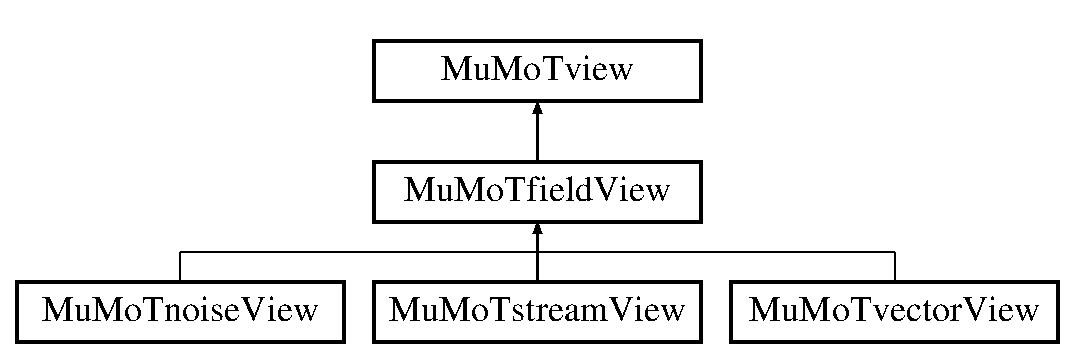
\includegraphics[height=3.000000cm]{class_mu_mo_t_1_1_mu_mo_t_1_1_mu_mo_tfield_view}
\end{center}
\end{figure}
\subsection*{Public Member Functions}
\begin{DoxyCompactItemize}
\item 
def \hyperlink{class_mu_mo_t_1_1_mu_mo_t_1_1_mu_mo_tfield_view_a78d68546a28ea07c46f5f4a44ddfa49a}{\+\_\+\+\_\+init\+\_\+\+\_\+} (self, model, controller, state\+Variable1, state\+Variable2, state\+Variable3=None, figure=None, params=None, kwargs)
\end{DoxyCompactItemize}
\subsection*{Static Public Attributes}
\begin{DoxyCompactItemize}
\item 
int \hyperlink{class_mu_mo_t_1_1_mu_mo_t_1_1_mu_mo_tfield_view_ab77cc972f3ee899689ba053015472ccd}{mask} = 1
\item 
\hyperlink{class_mu_mo_t_1_1_mu_mo_t_1_1_mu_mo_tfield_view_a5d76cc2129e79ba1941d2cc2f53b9e8e}{mask}
\end{DoxyCompactItemize}
\subsection*{Private Member Functions}
\begin{DoxyCompactItemize}
\item 
def \hyperlink{class_mu_mo_t_1_1_mu_mo_t_1_1_mu_mo_tfield_view_a118471f0e7fd4912146ed08084aa4b52}{\+\_\+build\+\_\+bookmark} (self)
\item 
def \hyperlink{class_mu_mo_t_1_1_mu_mo_t_1_1_mu_mo_tfield_view_a50d59419298116f738a98c864afb9d89}{\+\_\+plot\+\_\+field} (self)
\begin{DoxyCompactList}\small\item\em calculates stationary states of 2d system def \+\_\+get\+\_\+fixed\+Points2d(self)\+: \#plot\+Limits = self.\+\_\+controller.\+\_\+get\+Plot\+Limits() if self.\+\_\+controller != None\+: param\+Names = \mbox{[}\mbox{]} param\+Values = \mbox{[}\mbox{]} for name, value in self.\+\_\+controller.\+\_\+widgets\+Free\+Params.\+items()\+: \subsection*{throw away formatting for constant reactants}

\subsection*{name = name.\+replace(\textquotesingle{}(\textquotesingle{},\textquotesingle{}\textquotesingle{})}

\subsection*{name = name.\+replace(\textquotesingle{})\textquotesingle{},\textquotesingle{}\textquotesingle{})}

param\+Names.\+append(name) param\+Values.\+append(value.\+value) else\+: param\+Names = map(str, self.\+\_\+param\+Names) param\+Values = self.\+\_\+param\+Values funcs = self.\+\_\+mumot\+Model.\+\_\+get\+Funcs() arg\+Names\+Symb = list(map(\+Symbol, param\+Names)) arg\+Dict = dict(zip(arg\+Names\+Symb, param\+Values)) arg\+Dict\mbox{[}self.\+\_\+mumot\+Model.\+\_\+system\+Size\mbox{]} = 1 \end{DoxyCompactList}\item 
def \hyperlink{class_mu_mo_t_1_1_mu_mo_t_1_1_mu_mo_tfield_view_aefbf0e354438e17ab6d48e2d368f8540}{\+\_\+get\+\_\+field} (self)
\begin{DoxyCompactList}\small\item\em helper for \+\_\+get\+\_\+field\+\_\+2d() and \+\_\+get\+\_\+field\+\_\+3d() \end{DoxyCompactList}\item 
def \hyperlink{class_mu_mo_t_1_1_mu_mo_t_1_1_mu_mo_tfield_view_afb80cbad7f52c6df0abcb919739ee4de}{\+\_\+get\+\_\+field2d} (self, kind, mesh\+Points, plot\+Limits=1)
\begin{DoxyCompactList}\small\item\em get 2-\/dimensional field for plotting \end{DoxyCompactList}\item 
def \hyperlink{class_mu_mo_t_1_1_mu_mo_t_1_1_mu_mo_tfield_view_a4e3fec079e943d1c0e69b5f7e3f58565}{\+\_\+get\+\_\+field3d} (self, kind, mesh\+Points, plot\+Limits=1)
\begin{DoxyCompactList}\small\item\em get 3-\/dimensional field for plotting \end{DoxyCompactList}\end{DoxyCompactItemize}
\subsection*{Private Attributes}
\begin{DoxyCompactItemize}
\item 
\hyperlink{class_mu_mo_t_1_1_mu_mo_t_1_1_mu_mo_tfield_view_a6a353a1ef9443ae375948d592ed6cec6}{\+\_\+choose\+Font\+Size}
\item 
\hyperlink{class_mu_mo_t_1_1_mu_mo_t_1_1_mu_mo_tfield_view_ac83a924ad62a2461d65b5c9bf9d27453}{\+\_\+show\+Fixed\+Points}
\item 
\hyperlink{class_mu_mo_t_1_1_mu_mo_t_1_1_mu_mo_tfield_view_a865b2109ba10d874e84d4a354873b121}{\+\_\+xlab}
\item 
\hyperlink{class_mu_mo_t_1_1_mu_mo_t_1_1_mu_mo_tfield_view_aac1a25a634d53e524573f67eb5f3a7b9}{\+\_\+ylab}
\item 
\hyperlink{class_mu_mo_t_1_1_mu_mo_t_1_1_mu_mo_tfield_view_afcc07605f40039b605802f93b39ea910}{\+\_\+zlab}
\item 
\hyperlink{class_mu_mo_t_1_1_mu_mo_t_1_1_mu_mo_tfield_view_a506ccaeadc9c6f4102cf4e06f5a6be2a}{\+\_\+axes3d}
\end{DoxyCompactItemize}
\subsection*{Static Private Attributes}
\begin{DoxyCompactItemize}
\item 
\hyperlink{class_mu_mo_t_1_1_mu_mo_t_1_1_mu_mo_tfield_view_aa14fa36730691becc6f3136899545416}{\+\_\+state\+Variable1} = None
\begin{DoxyCompactList}\small\item\em 1st state variable (x-\/dimension) \end{DoxyCompactList}\item 
\hyperlink{class_mu_mo_t_1_1_mu_mo_t_1_1_mu_mo_tfield_view_a9d3705d1d9182e10751ff693573d6d16}{\+\_\+state\+Variable2} = None
\begin{DoxyCompactList}\small\item\em 2nd state variable (y-\/dimension) \end{DoxyCompactList}\item 
\hyperlink{class_mu_mo_t_1_1_mu_mo_t_1_1_mu_mo_tfield_view_ad2f8dc44173a16468bd9d3ab335f9b27}{\+\_\+state\+Variable3} = None
\begin{DoxyCompactList}\small\item\em 3rd state variable (z-\/dimension) \end{DoxyCompactList}\item 
\hyperlink{class_mu_mo_t_1_1_mu_mo_t_1_1_mu_mo_tfield_view_abb529af75494ab2513e57b8434c7c975}{\+\_\+X} = None
\begin{DoxyCompactList}\small\item\em X ordinates array. \end{DoxyCompactList}\item 
\hyperlink{class_mu_mo_t_1_1_mu_mo_t_1_1_mu_mo_tfield_view_a17bd9f55d983ee8d5a6f22088d0397e8}{\+\_\+Y} = None
\begin{DoxyCompactList}\small\item\em Y ordinates array. \end{DoxyCompactList}\item 
\hyperlink{class_mu_mo_t_1_1_mu_mo_t_1_1_mu_mo_tfield_view_a7b96cbb62a4ad08851fa147958f0d6e4}{\+\_\+Z} = None
\begin{DoxyCompactList}\small\item\em Z ordinates array. \end{DoxyCompactList}\item 
\hyperlink{class_mu_mo_t_1_1_mu_mo_t_1_1_mu_mo_tfield_view_a3293b40663039bb46c8c977a9948436e}{\+\_\+speed} = None
\begin{DoxyCompactList}\small\item\em speed array \end{DoxyCompactList}\item 
dictionary \hyperlink{class_mu_mo_t_1_1_mu_mo_t_1_1_mu_mo_tfield_view_acbf4bc8fa26c3cf9e1d2741cc3dea058}{\+\_\+mask} = \{\}
\begin{DoxyCompactList}\small\item\em class-\/global dictionary of memoised masks with (mesh size, dimension) as key \end{DoxyCompactList}\item 
\hyperlink{class_mu_mo_t_1_1_mu_mo_t_1_1_mu_mo_tfield_view_a0f5fba57766067c941f5a96b22545ed4}{\+\_\+\+Xdot}
\item 
\hyperlink{class_mu_mo_t_1_1_mu_mo_t_1_1_mu_mo_tfield_view_a31f5ad9d4a349b00e06772177200c217}{\+\_\+\+Ydot}
\item 
\hyperlink{class_mu_mo_t_1_1_mu_mo_t_1_1_mu_mo_tfield_view_a4008c2e6651cb1bf1c9c1af3e962a25d}{\+\_\+\+Zdot}
\end{DoxyCompactItemize}


\subsection{Detailed Description}
field view on model (specialised by \hyperlink{class_mu_mo_t_1_1_mu_mo_t_1_1_mu_mo_tvector_view}{Mu\+Mo\+Tvector\+View} and \hyperlink{class_mu_mo_t_1_1_mu_mo_t_1_1_mu_mo_tstream_view}{Mu\+Mo\+Tstream\+View}) 

\subsection{Constructor \& Destructor Documentation}
\mbox{\Hypertarget{class_mu_mo_t_1_1_mu_mo_t_1_1_mu_mo_tfield_view_a78d68546a28ea07c46f5f4a44ddfa49a}\label{class_mu_mo_t_1_1_mu_mo_t_1_1_mu_mo_tfield_view_a78d68546a28ea07c46f5f4a44ddfa49a}} 
\index{Mu\+Mo\+T\+::\+Mu\+Mo\+T\+::\+Mu\+Mo\+Tfield\+View@{Mu\+Mo\+T\+::\+Mu\+Mo\+T\+::\+Mu\+Mo\+Tfield\+View}!\+\_\+\+\_\+init\+\_\+\+\_\+@{\+\_\+\+\_\+init\+\_\+\+\_\+}}
\index{\+\_\+\+\_\+init\+\_\+\+\_\+@{\+\_\+\+\_\+init\+\_\+\+\_\+}!Mu\+Mo\+T\+::\+Mu\+Mo\+T\+::\+Mu\+Mo\+Tfield\+View@{Mu\+Mo\+T\+::\+Mu\+Mo\+T\+::\+Mu\+Mo\+Tfield\+View}}
\subsubsection{\texorpdfstring{\+\_\+\+\_\+init\+\_\+\+\_\+()}{\_\_init\_\_()}}
{\footnotesize\ttfamily def \+\_\+\+\_\+init\+\_\+\+\_\+ (\begin{DoxyParamCaption}\item[{}]{self,  }\item[{}]{model,  }\item[{}]{controller,  }\item[{}]{state\+Variable1,  }\item[{}]{state\+Variable2,  }\item[{}]{state\+Variable3 = {\ttfamily None},  }\item[{}]{figure = {\ttfamily None},  }\item[{}]{params = {\ttfamily None},  }\item[{}]{kwargs }\end{DoxyParamCaption})}



\subsection{Member Function Documentation}
\mbox{\Hypertarget{class_mu_mo_t_1_1_mu_mo_t_1_1_mu_mo_tfield_view_a118471f0e7fd4912146ed08084aa4b52}\label{class_mu_mo_t_1_1_mu_mo_t_1_1_mu_mo_tfield_view_a118471f0e7fd4912146ed08084aa4b52}} 
\index{Mu\+Mo\+T\+::\+Mu\+Mo\+T\+::\+Mu\+Mo\+Tfield\+View@{Mu\+Mo\+T\+::\+Mu\+Mo\+T\+::\+Mu\+Mo\+Tfield\+View}!\+\_\+build\+\_\+bookmark@{\+\_\+build\+\_\+bookmark}}
\index{\+\_\+build\+\_\+bookmark@{\+\_\+build\+\_\+bookmark}!Mu\+Mo\+T\+::\+Mu\+Mo\+T\+::\+Mu\+Mo\+Tfield\+View@{Mu\+Mo\+T\+::\+Mu\+Mo\+T\+::\+Mu\+Mo\+Tfield\+View}}
\subsubsection{\texorpdfstring{\+\_\+build\+\_\+bookmark()}{\_build\_bookmark()}}
{\footnotesize\ttfamily def \+\_\+build\+\_\+bookmark (\begin{DoxyParamCaption}\item[{}]{self }\end{DoxyParamCaption})\hspace{0.3cm}{\ttfamily [private]}}

\mbox{\Hypertarget{class_mu_mo_t_1_1_mu_mo_t_1_1_mu_mo_tfield_view_aefbf0e354438e17ab6d48e2d368f8540}\label{class_mu_mo_t_1_1_mu_mo_t_1_1_mu_mo_tfield_view_aefbf0e354438e17ab6d48e2d368f8540}} 
\index{Mu\+Mo\+T\+::\+Mu\+Mo\+T\+::\+Mu\+Mo\+Tfield\+View@{Mu\+Mo\+T\+::\+Mu\+Mo\+T\+::\+Mu\+Mo\+Tfield\+View}!\+\_\+get\+\_\+field@{\+\_\+get\+\_\+field}}
\index{\+\_\+get\+\_\+field@{\+\_\+get\+\_\+field}!Mu\+Mo\+T\+::\+Mu\+Mo\+T\+::\+Mu\+Mo\+Tfield\+View@{Mu\+Mo\+T\+::\+Mu\+Mo\+T\+::\+Mu\+Mo\+Tfield\+View}}
\subsubsection{\texorpdfstring{\+\_\+get\+\_\+field()}{\_get\_field()}}
{\footnotesize\ttfamily def \+\_\+get\+\_\+field (\begin{DoxyParamCaption}\item[{}]{self }\end{DoxyParamCaption})\hspace{0.3cm}{\ttfamily [private]}}



helper for \+\_\+get\+\_\+field\+\_\+2d() and \+\_\+get\+\_\+field\+\_\+3d() 

\mbox{\Hypertarget{class_mu_mo_t_1_1_mu_mo_t_1_1_mu_mo_tfield_view_afb80cbad7f52c6df0abcb919739ee4de}\label{class_mu_mo_t_1_1_mu_mo_t_1_1_mu_mo_tfield_view_afb80cbad7f52c6df0abcb919739ee4de}} 
\index{Mu\+Mo\+T\+::\+Mu\+Mo\+T\+::\+Mu\+Mo\+Tfield\+View@{Mu\+Mo\+T\+::\+Mu\+Mo\+T\+::\+Mu\+Mo\+Tfield\+View}!\+\_\+get\+\_\+field2d@{\+\_\+get\+\_\+field2d}}
\index{\+\_\+get\+\_\+field2d@{\+\_\+get\+\_\+field2d}!Mu\+Mo\+T\+::\+Mu\+Mo\+T\+::\+Mu\+Mo\+Tfield\+View@{Mu\+Mo\+T\+::\+Mu\+Mo\+T\+::\+Mu\+Mo\+Tfield\+View}}
\subsubsection{\texorpdfstring{\+\_\+get\+\_\+field2d()}{\_get\_field2d()}}
{\footnotesize\ttfamily def \+\_\+get\+\_\+field2d (\begin{DoxyParamCaption}\item[{}]{self,  }\item[{}]{kind,  }\item[{}]{mesh\+Points,  }\item[{}]{plot\+Limits = {\ttfamily 1} }\end{DoxyParamCaption})\hspace{0.3cm}{\ttfamily [private]}}



get 2-\/dimensional field for plotting 

\mbox{\Hypertarget{class_mu_mo_t_1_1_mu_mo_t_1_1_mu_mo_tfield_view_a4e3fec079e943d1c0e69b5f7e3f58565}\label{class_mu_mo_t_1_1_mu_mo_t_1_1_mu_mo_tfield_view_a4e3fec079e943d1c0e69b5f7e3f58565}} 
\index{Mu\+Mo\+T\+::\+Mu\+Mo\+T\+::\+Mu\+Mo\+Tfield\+View@{Mu\+Mo\+T\+::\+Mu\+Mo\+T\+::\+Mu\+Mo\+Tfield\+View}!\+\_\+get\+\_\+field3d@{\+\_\+get\+\_\+field3d}}
\index{\+\_\+get\+\_\+field3d@{\+\_\+get\+\_\+field3d}!Mu\+Mo\+T\+::\+Mu\+Mo\+T\+::\+Mu\+Mo\+Tfield\+View@{Mu\+Mo\+T\+::\+Mu\+Mo\+T\+::\+Mu\+Mo\+Tfield\+View}}
\subsubsection{\texorpdfstring{\+\_\+get\+\_\+field3d()}{\_get\_field3d()}}
{\footnotesize\ttfamily def \+\_\+get\+\_\+field3d (\begin{DoxyParamCaption}\item[{}]{self,  }\item[{}]{kind,  }\item[{}]{mesh\+Points,  }\item[{}]{plot\+Limits = {\ttfamily 1} }\end{DoxyParamCaption})\hspace{0.3cm}{\ttfamily [private]}}



get 3-\/dimensional field for plotting 

\mbox{\Hypertarget{class_mu_mo_t_1_1_mu_mo_t_1_1_mu_mo_tfield_view_a50d59419298116f738a98c864afb9d89}\label{class_mu_mo_t_1_1_mu_mo_t_1_1_mu_mo_tfield_view_a50d59419298116f738a98c864afb9d89}} 
\index{Mu\+Mo\+T\+::\+Mu\+Mo\+T\+::\+Mu\+Mo\+Tfield\+View@{Mu\+Mo\+T\+::\+Mu\+Mo\+T\+::\+Mu\+Mo\+Tfield\+View}!\+\_\+plot\+\_\+field@{\+\_\+plot\+\_\+field}}
\index{\+\_\+plot\+\_\+field@{\+\_\+plot\+\_\+field}!Mu\+Mo\+T\+::\+Mu\+Mo\+T\+::\+Mu\+Mo\+Tfield\+View@{Mu\+Mo\+T\+::\+Mu\+Mo\+T\+::\+Mu\+Mo\+Tfield\+View}}
\subsubsection{\texorpdfstring{\+\_\+plot\+\_\+field()}{\_plot\_field()}}
{\footnotesize\ttfamily def \+\_\+plot\+\_\+field (\begin{DoxyParamCaption}\item[{}]{self }\end{DoxyParamCaption})\hspace{0.3cm}{\ttfamily [private]}}



calculates stationary states of 2d system def \+\_\+get\+\_\+fixed\+Points2d(self)\+: \#plot\+Limits = self.\+\_\+controller.\+\_\+get\+Plot\+Limits() if self.\+\_\+controller != None\+: param\+Names = \mbox{[}\mbox{]} param\+Values = \mbox{[}\mbox{]} for name, value in self.\+\_\+controller.\+\_\+widgets\+Free\+Params.\+items()\+: \subsection*{throw away formatting for constant reactants}

\subsection*{name = name.\+replace(\textquotesingle{}(\textquotesingle{},\textquotesingle{}\textquotesingle{})}

\subsection*{name = name.\+replace(\textquotesingle{})\textquotesingle{},\textquotesingle{}\textquotesingle{})}

param\+Names.\+append(name) param\+Values.\+append(value.\+value) else\+: param\+Names = map(str, self.\+\_\+param\+Names) param\+Values = self.\+\_\+param\+Values funcs = self.\+\_\+mumot\+Model.\+\_\+get\+Funcs() arg\+Names\+Symb = list(map(\+Symbol, param\+Names)) arg\+Dict = dict(zip(arg\+Names\+Symb, param\+Values)) arg\+Dict\mbox{[}self.\+\_\+mumot\+Model.\+\_\+system\+Size\mbox{]} = 1 

\subsection*{if self.\+\_\+controller != None\+:}

\subsection*{param\+Names = \mbox{[}\mbox{]}}

\subsection*{param\+Values = \mbox{[}\mbox{]}}

\subsection*{for name, value in self.\+\_\+controller.\+\_\+widgets\+Free\+Params.\+items()\+:}

\subsection*{param\+Names.\+append(name)}

\subsection*{param\+Values.\+append(value.\+value)}

\subsection*{else\+:}

\subsection*{param\+Names = map(str, self.\+\_\+param\+Names)}

\subsection*{param\+Values = self.\+\_\+param\+Values}

\subsection*{}

\subsection*{arg\+Names\+Symb = list(map(\+Symbol, param\+Names))}

\subsection*{arg\+Dict = dict(zip(arg\+Names\+Symb, param\+Values))}

\subsection*{arg\+Dict\mbox{[}self.\+\_\+mumot\+Model.\+\_\+system\+Size\mbox{]} = 1}

\begin{DoxyVerb}    EQ1 = self._mumotModel._equations[self._stateVariable1].subs(argDict)
    EQ2 = self._mumotModel._equations[self._stateVariable2].subs(argDict)
    eps=1e-8
    EQsol = solve((EQ1, EQ2), (self._stateVariable1, self._stateVariable2), dict=True)
    #for kk in range(len(EQsol)):
    #    print(EQsol[kk])
    realEQsol = [{self._stateVariable1: re(EQsol[kk][self._stateVariable1]), self._stateVariable2: re(EQsol[kk][self._stateVariable2])} for kk in range(len(EQsol)) if (Abs(im(EQsol[kk][self._stateVariable1]))<=eps and Abs(im(EQsol[kk][self._stateVariable2]))<=eps)]

    MAT = Matrix([EQ1, EQ2])
    JAC = MAT.jacobian([self._stateVariable1,self._stateVariable2])

    eigList = []
    #for nn in range(len(realEQsol)): 
    #    JACsub=JAC.subs([(self._stateVariable1, realEQsol[nn][self._stateVariable1]), (self._stateVariable2, realEQsol[nn][self._stateVariable2])])
    #    evSet = JACsub.eigenvals()
    #    eigList.append(evSet)
    for nn in range(len(realEQsol)): 
        evSet = {}
        JACsub=JAC.subs([(self._stateVariable1, realEQsol[nn][self._stateVariable1]), (self._stateVariable2, realEQsol[nn][self._stateVariable2])])
        #evSet = JACsub.eigenvals()
        eigVects = JACsub.eigenvects()
        for kk in range(len(eigVects)):
            evSet[eigVects[kk][0]] = (eigVects[kk][1], eigVects[kk][2])
        eigList.append(evSet)
    return realEQsol, eigList #returns two lists of dictionaries

## calculates stationary states of 3d system
def _get_fixedPoints3d(self):
    #plotLimits = self._controller._getPlotLimits()
    if self._controller != None:
        paramNames = []
        paramValues = []
        for name, value in self._controller._widgetsFreeParams.items():
            # throw away formatting for constant reactants
\end{DoxyVerb}
 \subsection*{name = name.\+replace(\textquotesingle{}(\textquotesingle{},\textquotesingle{}\textquotesingle{})}

\subsection*{name = name.\+replace(\textquotesingle{})\textquotesingle{},\textquotesingle{}\textquotesingle{})}

param\+Names.\+append(name) param\+Values.\+append(value.\+value) else\+: param\+Names = map(str, self.\+\_\+param\+Names) param\+Values = self.\+\_\+param\+Values funcs = self.\+\_\+mumot\+Model.\+\_\+get\+Funcs() arg\+Names\+Symb = list(map(\+Symbol, param\+Names)) arg\+Dict = dict(zip(arg\+Names\+Symb, param\+Values)) arg\+Dict\mbox{[}self.\+\_\+mumot\+Model.\+\_\+system\+Size\mbox{]} = 1

\subsection*{if self.\+\_\+controller != None\+:}

\subsection*{param\+Names = \mbox{[}\mbox{]}}

\subsection*{param\+Values = \mbox{[}\mbox{]}}

\subsection*{for name, value in self.\+\_\+controller.\+\_\+widgets\+Free\+Params.\+items()\+:}

\subsection*{param\+Names.\+append(name)}

\subsection*{param\+Values.\+append(value.\+value)}

\subsection*{else\+:}

\subsection*{param\+Names = map(str, self.\+\_\+param\+Names)}

\subsection*{param\+Values = self.\+\_\+param\+Values}

\subsection*{}

\subsection*{arg\+Names\+Symb = list(map(\+Symbol, param\+Names))}

\subsection*{arg\+Dict = dict(zip(arg\+Names\+Symb, param\+Values))}

\subsection*{arg\+Dict\mbox{[}self.\+\_\+mumot\+Model.\+\_\+system\+Size\mbox{]} = 1}

\begin{DoxyVerb}    EQ1 = self._mumotModel._equations[self._stateVariable1].subs(argDict)
    EQ2 = self._mumotModel._equations[self._stateVariable2].subs(argDict)
    EQ3 = self._mumotModel._equations[self._stateVariable3].subs(argDict)
    eps=1e-8
    EQsol = solve((EQ1, EQ2, EQ3), (self._stateVariable1, self._stateVariable2, self._stateVariable3), dict=True)
    realEQsol = [{self._stateVariable1: re(EQsol[kk][self._stateVariable1]), self._stateVariable2: re(EQsol[kk][self._stateVariable2]), self._stateVariable3: re(EQsol[kk][self._stateVariable3])} for kk in range(len(EQsol)) if (Abs(im(EQsol[kk][self._stateVariable1]))<=eps and Abs(im(EQsol[kk][self._stateVariable2]))<=eps and Abs(im(EQsol[kk][self._stateVariable3]))<=eps)]

    MAT = Matrix([EQ1, EQ2, EQ3])
    JAC = MAT.jacobian([self._stateVariable1,self._stateVariable2,self._stateVariable3])

    eigList = []
    #for nn in range(len(realEQsol)): 
    #    JACsub=JAC.subs([(self._stateVariable1, realEQsol[nn][self._stateVariable1]), (self._stateVariable2, realEQsol[nn][self._stateVariable2]), (self._stateVariable3, realEQsol[nn][self._stateVariable3])])
    #    evSet = JACsub.eigenvals()
    #    eigList.append(evSet)
    for nn in range(len(realEQsol)): 
        evSet = {}
        JACsub=JAC.subs([(self._stateVariable1, realEQsol[nn][self._stateVariable1]), (self._stateVariable2, realEQsol[nn][self._stateVariable2]), (self._stateVariable3, realEQsol[nn][self._stateVariable3])])
        #evSet = JACsub.eigenvals()
        eigVects = JACsub.eigenvects()
        for kk in range(len(eigVects)):
            evSet[eigVects[kk][0]] = (eigVects[kk][1], eigVects[kk][2])
        eigList.append(evSet)
    return realEQsol, eigList #returns two lists of dictionaries \end{DoxyVerb}
 

\subsection{Field Documentation}
\mbox{\Hypertarget{class_mu_mo_t_1_1_mu_mo_t_1_1_mu_mo_tfield_view_a506ccaeadc9c6f4102cf4e06f5a6be2a}\label{class_mu_mo_t_1_1_mu_mo_t_1_1_mu_mo_tfield_view_a506ccaeadc9c6f4102cf4e06f5a6be2a}} 
\index{Mu\+Mo\+T\+::\+Mu\+Mo\+T\+::\+Mu\+Mo\+Tfield\+View@{Mu\+Mo\+T\+::\+Mu\+Mo\+T\+::\+Mu\+Mo\+Tfield\+View}!\+\_\+axes3d@{\+\_\+axes3d}}
\index{\+\_\+axes3d@{\+\_\+axes3d}!Mu\+Mo\+T\+::\+Mu\+Mo\+T\+::\+Mu\+Mo\+Tfield\+View@{Mu\+Mo\+T\+::\+Mu\+Mo\+T\+::\+Mu\+Mo\+Tfield\+View}}
\subsubsection{\texorpdfstring{\+\_\+axes3d}{\_axes3d}}
{\footnotesize\ttfamily \+\_\+axes3d\hspace{0.3cm}{\ttfamily [private]}}

\mbox{\Hypertarget{class_mu_mo_t_1_1_mu_mo_t_1_1_mu_mo_tfield_view_a6a353a1ef9443ae375948d592ed6cec6}\label{class_mu_mo_t_1_1_mu_mo_t_1_1_mu_mo_tfield_view_a6a353a1ef9443ae375948d592ed6cec6}} 
\index{Mu\+Mo\+T\+::\+Mu\+Mo\+T\+::\+Mu\+Mo\+Tfield\+View@{Mu\+Mo\+T\+::\+Mu\+Mo\+T\+::\+Mu\+Mo\+Tfield\+View}!\+\_\+choose\+Font\+Size@{\+\_\+choose\+Font\+Size}}
\index{\+\_\+choose\+Font\+Size@{\+\_\+choose\+Font\+Size}!Mu\+Mo\+T\+::\+Mu\+Mo\+T\+::\+Mu\+Mo\+Tfield\+View@{Mu\+Mo\+T\+::\+Mu\+Mo\+T\+::\+Mu\+Mo\+Tfield\+View}}
\subsubsection{\texorpdfstring{\+\_\+choose\+Font\+Size}{\_chooseFontSize}}
{\footnotesize\ttfamily \+\_\+choose\+Font\+Size\hspace{0.3cm}{\ttfamily [private]}}

\mbox{\Hypertarget{class_mu_mo_t_1_1_mu_mo_t_1_1_mu_mo_tfield_view_acbf4bc8fa26c3cf9e1d2741cc3dea058}\label{class_mu_mo_t_1_1_mu_mo_t_1_1_mu_mo_tfield_view_acbf4bc8fa26c3cf9e1d2741cc3dea058}} 
\index{Mu\+Mo\+T\+::\+Mu\+Mo\+T\+::\+Mu\+Mo\+Tfield\+View@{Mu\+Mo\+T\+::\+Mu\+Mo\+T\+::\+Mu\+Mo\+Tfield\+View}!\+\_\+mask@{\+\_\+mask}}
\index{\+\_\+mask@{\+\_\+mask}!Mu\+Mo\+T\+::\+Mu\+Mo\+T\+::\+Mu\+Mo\+Tfield\+View@{Mu\+Mo\+T\+::\+Mu\+Mo\+T\+::\+Mu\+Mo\+Tfield\+View}}
\subsubsection{\texorpdfstring{\+\_\+mask}{\_mask}}
{\footnotesize\ttfamily dictionary \+\_\+mask = \{\}\hspace{0.3cm}{\ttfamily [static]}, {\ttfamily [private]}}



class-\/global dictionary of memoised masks with (mesh size, dimension) as key 

\mbox{\Hypertarget{class_mu_mo_t_1_1_mu_mo_t_1_1_mu_mo_tfield_view_ac83a924ad62a2461d65b5c9bf9d27453}\label{class_mu_mo_t_1_1_mu_mo_t_1_1_mu_mo_tfield_view_ac83a924ad62a2461d65b5c9bf9d27453}} 
\index{Mu\+Mo\+T\+::\+Mu\+Mo\+T\+::\+Mu\+Mo\+Tfield\+View@{Mu\+Mo\+T\+::\+Mu\+Mo\+T\+::\+Mu\+Mo\+Tfield\+View}!\+\_\+show\+Fixed\+Points@{\+\_\+show\+Fixed\+Points}}
\index{\+\_\+show\+Fixed\+Points@{\+\_\+show\+Fixed\+Points}!Mu\+Mo\+T\+::\+Mu\+Mo\+T\+::\+Mu\+Mo\+Tfield\+View@{Mu\+Mo\+T\+::\+Mu\+Mo\+T\+::\+Mu\+Mo\+Tfield\+View}}
\subsubsection{\texorpdfstring{\+\_\+show\+Fixed\+Points}{\_showFixedPoints}}
{\footnotesize\ttfamily \+\_\+show\+Fixed\+Points\hspace{0.3cm}{\ttfamily [private]}}

\mbox{\Hypertarget{class_mu_mo_t_1_1_mu_mo_t_1_1_mu_mo_tfield_view_a3293b40663039bb46c8c977a9948436e}\label{class_mu_mo_t_1_1_mu_mo_t_1_1_mu_mo_tfield_view_a3293b40663039bb46c8c977a9948436e}} 
\index{Mu\+Mo\+T\+::\+Mu\+Mo\+T\+::\+Mu\+Mo\+Tfield\+View@{Mu\+Mo\+T\+::\+Mu\+Mo\+T\+::\+Mu\+Mo\+Tfield\+View}!\+\_\+speed@{\+\_\+speed}}
\index{\+\_\+speed@{\+\_\+speed}!Mu\+Mo\+T\+::\+Mu\+Mo\+T\+::\+Mu\+Mo\+Tfield\+View@{Mu\+Mo\+T\+::\+Mu\+Mo\+T\+::\+Mu\+Mo\+Tfield\+View}}
\subsubsection{\texorpdfstring{\+\_\+speed}{\_speed}}
{\footnotesize\ttfamily \+\_\+speed = None\hspace{0.3cm}{\ttfamily [static]}, {\ttfamily [private]}}



speed array 

\mbox{\Hypertarget{class_mu_mo_t_1_1_mu_mo_t_1_1_mu_mo_tfield_view_aa14fa36730691becc6f3136899545416}\label{class_mu_mo_t_1_1_mu_mo_t_1_1_mu_mo_tfield_view_aa14fa36730691becc6f3136899545416}} 
\index{Mu\+Mo\+T\+::\+Mu\+Mo\+T\+::\+Mu\+Mo\+Tfield\+View@{Mu\+Mo\+T\+::\+Mu\+Mo\+T\+::\+Mu\+Mo\+Tfield\+View}!\+\_\+state\+Variable1@{\+\_\+state\+Variable1}}
\index{\+\_\+state\+Variable1@{\+\_\+state\+Variable1}!Mu\+Mo\+T\+::\+Mu\+Mo\+T\+::\+Mu\+Mo\+Tfield\+View@{Mu\+Mo\+T\+::\+Mu\+Mo\+T\+::\+Mu\+Mo\+Tfield\+View}}
\subsubsection{\texorpdfstring{\+\_\+state\+Variable1}{\_stateVariable1}}
{\footnotesize\ttfamily \+\_\+state\+Variable1 = None\hspace{0.3cm}{\ttfamily [static]}, {\ttfamily [private]}}



1st state variable (x-\/dimension) 

\mbox{\Hypertarget{class_mu_mo_t_1_1_mu_mo_t_1_1_mu_mo_tfield_view_a9d3705d1d9182e10751ff693573d6d16}\label{class_mu_mo_t_1_1_mu_mo_t_1_1_mu_mo_tfield_view_a9d3705d1d9182e10751ff693573d6d16}} 
\index{Mu\+Mo\+T\+::\+Mu\+Mo\+T\+::\+Mu\+Mo\+Tfield\+View@{Mu\+Mo\+T\+::\+Mu\+Mo\+T\+::\+Mu\+Mo\+Tfield\+View}!\+\_\+state\+Variable2@{\+\_\+state\+Variable2}}
\index{\+\_\+state\+Variable2@{\+\_\+state\+Variable2}!Mu\+Mo\+T\+::\+Mu\+Mo\+T\+::\+Mu\+Mo\+Tfield\+View@{Mu\+Mo\+T\+::\+Mu\+Mo\+T\+::\+Mu\+Mo\+Tfield\+View}}
\subsubsection{\texorpdfstring{\+\_\+state\+Variable2}{\_stateVariable2}}
{\footnotesize\ttfamily \+\_\+state\+Variable2 = None\hspace{0.3cm}{\ttfamily [static]}, {\ttfamily [private]}}



2nd state variable (y-\/dimension) 

\mbox{\Hypertarget{class_mu_mo_t_1_1_mu_mo_t_1_1_mu_mo_tfield_view_ad2f8dc44173a16468bd9d3ab335f9b27}\label{class_mu_mo_t_1_1_mu_mo_t_1_1_mu_mo_tfield_view_ad2f8dc44173a16468bd9d3ab335f9b27}} 
\index{Mu\+Mo\+T\+::\+Mu\+Mo\+T\+::\+Mu\+Mo\+Tfield\+View@{Mu\+Mo\+T\+::\+Mu\+Mo\+T\+::\+Mu\+Mo\+Tfield\+View}!\+\_\+state\+Variable3@{\+\_\+state\+Variable3}}
\index{\+\_\+state\+Variable3@{\+\_\+state\+Variable3}!Mu\+Mo\+T\+::\+Mu\+Mo\+T\+::\+Mu\+Mo\+Tfield\+View@{Mu\+Mo\+T\+::\+Mu\+Mo\+T\+::\+Mu\+Mo\+Tfield\+View}}
\subsubsection{\texorpdfstring{\+\_\+state\+Variable3}{\_stateVariable3}}
{\footnotesize\ttfamily \+\_\+state\+Variable3 = None\hspace{0.3cm}{\ttfamily [static]}, {\ttfamily [private]}}



3rd state variable (z-\/dimension) 

\mbox{\Hypertarget{class_mu_mo_t_1_1_mu_mo_t_1_1_mu_mo_tfield_view_abb529af75494ab2513e57b8434c7c975}\label{class_mu_mo_t_1_1_mu_mo_t_1_1_mu_mo_tfield_view_abb529af75494ab2513e57b8434c7c975}} 
\index{Mu\+Mo\+T\+::\+Mu\+Mo\+T\+::\+Mu\+Mo\+Tfield\+View@{Mu\+Mo\+T\+::\+Mu\+Mo\+T\+::\+Mu\+Mo\+Tfield\+View}!\+\_\+X@{\+\_\+X}}
\index{\+\_\+X@{\+\_\+X}!Mu\+Mo\+T\+::\+Mu\+Mo\+T\+::\+Mu\+Mo\+Tfield\+View@{Mu\+Mo\+T\+::\+Mu\+Mo\+T\+::\+Mu\+Mo\+Tfield\+View}}
\subsubsection{\texorpdfstring{\+\_\+X}{\_X}}
{\footnotesize\ttfamily \+\_\+X = None\hspace{0.3cm}{\ttfamily [static]}, {\ttfamily [private]}}



X ordinates array. 

X derivatives array. \mbox{\Hypertarget{class_mu_mo_t_1_1_mu_mo_t_1_1_mu_mo_tfield_view_a0f5fba57766067c941f5a96b22545ed4}\label{class_mu_mo_t_1_1_mu_mo_t_1_1_mu_mo_tfield_view_a0f5fba57766067c941f5a96b22545ed4}} 
\index{Mu\+Mo\+T\+::\+Mu\+Mo\+T\+::\+Mu\+Mo\+Tfield\+View@{Mu\+Mo\+T\+::\+Mu\+Mo\+T\+::\+Mu\+Mo\+Tfield\+View}!\+\_\+\+Xdot@{\+\_\+\+Xdot}}
\index{\+\_\+\+Xdot@{\+\_\+\+Xdot}!Mu\+Mo\+T\+::\+Mu\+Mo\+T\+::\+Mu\+Mo\+Tfield\+View@{Mu\+Mo\+T\+::\+Mu\+Mo\+T\+::\+Mu\+Mo\+Tfield\+View}}
\subsubsection{\texorpdfstring{\+\_\+\+Xdot}{\_Xdot}}
{\footnotesize\ttfamily \+\_\+\+Xdot\hspace{0.3cm}{\ttfamily [static]}, {\ttfamily [private]}}

\begin{DoxyRefDesc}{Todo}
\item[\hyperlink{todo__todo000038}{Todo}]\+: allow user to set mesh points with keyword \end{DoxyRefDesc}
\mbox{\Hypertarget{class_mu_mo_t_1_1_mu_mo_t_1_1_mu_mo_tfield_view_a865b2109ba10d874e84d4a354873b121}\label{class_mu_mo_t_1_1_mu_mo_t_1_1_mu_mo_tfield_view_a865b2109ba10d874e84d4a354873b121}} 
\index{Mu\+Mo\+T\+::\+Mu\+Mo\+T\+::\+Mu\+Mo\+Tfield\+View@{Mu\+Mo\+T\+::\+Mu\+Mo\+T\+::\+Mu\+Mo\+Tfield\+View}!\+\_\+xlab@{\+\_\+xlab}}
\index{\+\_\+xlab@{\+\_\+xlab}!Mu\+Mo\+T\+::\+Mu\+Mo\+T\+::\+Mu\+Mo\+Tfield\+View@{Mu\+Mo\+T\+::\+Mu\+Mo\+T\+::\+Mu\+Mo\+Tfield\+View}}
\subsubsection{\texorpdfstring{\+\_\+xlab}{\_xlab}}
{\footnotesize\ttfamily \+\_\+xlab\hspace{0.3cm}{\ttfamily [private]}}

\mbox{\Hypertarget{class_mu_mo_t_1_1_mu_mo_t_1_1_mu_mo_tfield_view_a17bd9f55d983ee8d5a6f22088d0397e8}\label{class_mu_mo_t_1_1_mu_mo_t_1_1_mu_mo_tfield_view_a17bd9f55d983ee8d5a6f22088d0397e8}} 
\index{Mu\+Mo\+T\+::\+Mu\+Mo\+T\+::\+Mu\+Mo\+Tfield\+View@{Mu\+Mo\+T\+::\+Mu\+Mo\+T\+::\+Mu\+Mo\+Tfield\+View}!\+\_\+Y@{\+\_\+Y}}
\index{\+\_\+Y@{\+\_\+Y}!Mu\+Mo\+T\+::\+Mu\+Mo\+T\+::\+Mu\+Mo\+Tfield\+View@{Mu\+Mo\+T\+::\+Mu\+Mo\+T\+::\+Mu\+Mo\+Tfield\+View}}
\subsubsection{\texorpdfstring{\+\_\+Y}{\_Y}}
{\footnotesize\ttfamily \+\_\+Y = None\hspace{0.3cm}{\ttfamily [static]}, {\ttfamily [private]}}



Y ordinates array. 

Y derivatives array. \mbox{\Hypertarget{class_mu_mo_t_1_1_mu_mo_t_1_1_mu_mo_tfield_view_a31f5ad9d4a349b00e06772177200c217}\label{class_mu_mo_t_1_1_mu_mo_t_1_1_mu_mo_tfield_view_a31f5ad9d4a349b00e06772177200c217}} 
\index{Mu\+Mo\+T\+::\+Mu\+Mo\+T\+::\+Mu\+Mo\+Tfield\+View@{Mu\+Mo\+T\+::\+Mu\+Mo\+T\+::\+Mu\+Mo\+Tfield\+View}!\+\_\+\+Ydot@{\+\_\+\+Ydot}}
\index{\+\_\+\+Ydot@{\+\_\+\+Ydot}!Mu\+Mo\+T\+::\+Mu\+Mo\+T\+::\+Mu\+Mo\+Tfield\+View@{Mu\+Mo\+T\+::\+Mu\+Mo\+T\+::\+Mu\+Mo\+Tfield\+View}}
\subsubsection{\texorpdfstring{\+\_\+\+Ydot}{\_Ydot}}
{\footnotesize\ttfamily \+\_\+\+Ydot\hspace{0.3cm}{\ttfamily [static]}, {\ttfamily [private]}}

\mbox{\Hypertarget{class_mu_mo_t_1_1_mu_mo_t_1_1_mu_mo_tfield_view_aac1a25a634d53e524573f67eb5f3a7b9}\label{class_mu_mo_t_1_1_mu_mo_t_1_1_mu_mo_tfield_view_aac1a25a634d53e524573f67eb5f3a7b9}} 
\index{Mu\+Mo\+T\+::\+Mu\+Mo\+T\+::\+Mu\+Mo\+Tfield\+View@{Mu\+Mo\+T\+::\+Mu\+Mo\+T\+::\+Mu\+Mo\+Tfield\+View}!\+\_\+ylab@{\+\_\+ylab}}
\index{\+\_\+ylab@{\+\_\+ylab}!Mu\+Mo\+T\+::\+Mu\+Mo\+T\+::\+Mu\+Mo\+Tfield\+View@{Mu\+Mo\+T\+::\+Mu\+Mo\+T\+::\+Mu\+Mo\+Tfield\+View}}
\subsubsection{\texorpdfstring{\+\_\+ylab}{\_ylab}}
{\footnotesize\ttfamily \+\_\+ylab\hspace{0.3cm}{\ttfamily [private]}}

\mbox{\Hypertarget{class_mu_mo_t_1_1_mu_mo_t_1_1_mu_mo_tfield_view_a7b96cbb62a4ad08851fa147958f0d6e4}\label{class_mu_mo_t_1_1_mu_mo_t_1_1_mu_mo_tfield_view_a7b96cbb62a4ad08851fa147958f0d6e4}} 
\index{Mu\+Mo\+T\+::\+Mu\+Mo\+T\+::\+Mu\+Mo\+Tfield\+View@{Mu\+Mo\+T\+::\+Mu\+Mo\+T\+::\+Mu\+Mo\+Tfield\+View}!\+\_\+Z@{\+\_\+Z}}
\index{\+\_\+Z@{\+\_\+Z}!Mu\+Mo\+T\+::\+Mu\+Mo\+T\+::\+Mu\+Mo\+Tfield\+View@{Mu\+Mo\+T\+::\+Mu\+Mo\+T\+::\+Mu\+Mo\+Tfield\+View}}
\subsubsection{\texorpdfstring{\+\_\+Z}{\_Z}}
{\footnotesize\ttfamily \+\_\+Z = None\hspace{0.3cm}{\ttfamily [static]}, {\ttfamily [private]}}



Z ordinates array. 

Z derivatives array. \mbox{\Hypertarget{class_mu_mo_t_1_1_mu_mo_t_1_1_mu_mo_tfield_view_a4008c2e6651cb1bf1c9c1af3e962a25d}\label{class_mu_mo_t_1_1_mu_mo_t_1_1_mu_mo_tfield_view_a4008c2e6651cb1bf1c9c1af3e962a25d}} 
\index{Mu\+Mo\+T\+::\+Mu\+Mo\+T\+::\+Mu\+Mo\+Tfield\+View@{Mu\+Mo\+T\+::\+Mu\+Mo\+T\+::\+Mu\+Mo\+Tfield\+View}!\+\_\+\+Zdot@{\+\_\+\+Zdot}}
\index{\+\_\+\+Zdot@{\+\_\+\+Zdot}!Mu\+Mo\+T\+::\+Mu\+Mo\+T\+::\+Mu\+Mo\+Tfield\+View@{Mu\+Mo\+T\+::\+Mu\+Mo\+T\+::\+Mu\+Mo\+Tfield\+View}}
\subsubsection{\texorpdfstring{\+\_\+\+Zdot}{\_Zdot}}
{\footnotesize\ttfamily \+\_\+\+Zdot\hspace{0.3cm}{\ttfamily [static]}, {\ttfamily [private]}}

\mbox{\Hypertarget{class_mu_mo_t_1_1_mu_mo_t_1_1_mu_mo_tfield_view_afcc07605f40039b605802f93b39ea910}\label{class_mu_mo_t_1_1_mu_mo_t_1_1_mu_mo_tfield_view_afcc07605f40039b605802f93b39ea910}} 
\index{Mu\+Mo\+T\+::\+Mu\+Mo\+T\+::\+Mu\+Mo\+Tfield\+View@{Mu\+Mo\+T\+::\+Mu\+Mo\+T\+::\+Mu\+Mo\+Tfield\+View}!\+\_\+zlab@{\+\_\+zlab}}
\index{\+\_\+zlab@{\+\_\+zlab}!Mu\+Mo\+T\+::\+Mu\+Mo\+T\+::\+Mu\+Mo\+Tfield\+View@{Mu\+Mo\+T\+::\+Mu\+Mo\+T\+::\+Mu\+Mo\+Tfield\+View}}
\subsubsection{\texorpdfstring{\+\_\+zlab}{\_zlab}}
{\footnotesize\ttfamily \+\_\+zlab\hspace{0.3cm}{\ttfamily [private]}}

\mbox{\Hypertarget{class_mu_mo_t_1_1_mu_mo_t_1_1_mu_mo_tfield_view_ab77cc972f3ee899689ba053015472ccd}\label{class_mu_mo_t_1_1_mu_mo_t_1_1_mu_mo_tfield_view_ab77cc972f3ee899689ba053015472ccd}} 
\index{Mu\+Mo\+T\+::\+Mu\+Mo\+T\+::\+Mu\+Mo\+Tfield\+View@{Mu\+Mo\+T\+::\+Mu\+Mo\+T\+::\+Mu\+Mo\+Tfield\+View}!mask@{mask}}
\index{mask@{mask}!Mu\+Mo\+T\+::\+Mu\+Mo\+T\+::\+Mu\+Mo\+Tfield\+View@{Mu\+Mo\+T\+::\+Mu\+Mo\+T\+::\+Mu\+Mo\+Tfield\+View}}
\subsubsection{\texorpdfstring{mask}{mask}\hspace{0.1cm}{\footnotesize\ttfamily [1/2]}}
{\footnotesize\ttfamily int mask = 1\hspace{0.3cm}{\ttfamily [static]}}

\mbox{\Hypertarget{class_mu_mo_t_1_1_mu_mo_t_1_1_mu_mo_tfield_view_a5d76cc2129e79ba1941d2cc2f53b9e8e}\label{class_mu_mo_t_1_1_mu_mo_t_1_1_mu_mo_tfield_view_a5d76cc2129e79ba1941d2cc2f53b9e8e}} 
\index{Mu\+Mo\+T\+::\+Mu\+Mo\+T\+::\+Mu\+Mo\+Tfield\+View@{Mu\+Mo\+T\+::\+Mu\+Mo\+T\+::\+Mu\+Mo\+Tfield\+View}!mask@{mask}}
\index{mask@{mask}!Mu\+Mo\+T\+::\+Mu\+Mo\+T\+::\+Mu\+Mo\+Tfield\+View@{Mu\+Mo\+T\+::\+Mu\+Mo\+T\+::\+Mu\+Mo\+Tfield\+View}}
\subsubsection{\texorpdfstring{mask}{mask}\hspace{0.1cm}{\footnotesize\ttfamily [2/2]}}
{\footnotesize\ttfamily mask\hspace{0.3cm}{\ttfamily [static]}}



The documentation for this class was generated from the following file\+:\begin{DoxyCompactItemize}
\item 
Mu\+Mo\+T/\hyperlink{_mu_mo_t_8py}{Mu\+Mo\+T.\+py}\end{DoxyCompactItemize}

\hypertarget{class_mu_mo_t_1_1_mu_mo_t_1_1_mu_mo_tmodel}{}\section{Mu\+Mo\+Tmodel Class Reference}
\label{class_mu_mo_t_1_1_mu_mo_t_1_1_mu_mo_tmodel}\index{Mu\+Mo\+Tmodel@{Mu\+Mo\+Tmodel}}


class describing a model  


\subsection*{Public Member Functions}
\begin{DoxyCompactItemize}
\item 
def \hyperlink{class_mu_mo_t_1_1_mu_mo_t_1_1_mu_mo_tmodel_a2eec4a3b8deda7c717c06ed89c24d570}{substitute} (self, subs\+String)
\begin{DoxyCompactList}\small\item\em create new model with variable substitutions listed as comma separated string of assignments \end{DoxyCompactList}\item 
def \hyperlink{class_mu_mo_t_1_1_mu_mo_t_1_1_mu_mo_tmodel_affc6fae7ea26f85cde5366af8af85200}{visualise} (self)
\begin{DoxyCompactList}\small\item\em build a graphical representation of the model if result cannot be plotted check for installation of libltdl -\/ eg on Mac see if X\+Quartz requires update or do\+:~\newline
 {\ttfamily brew install libtool -\/-\/universal} ~\newline
 {\ttfamily brew link libtool} \end{DoxyCompactList}\item 
def \hyperlink{class_mu_mo_t_1_1_mu_mo_t_1_1_mu_mo_tmodel_a824eaf8994c839c0a9f17539f298974f}{show\+Constant\+Reactants} (self)
\begin{DoxyCompactList}\small\item\em show a sorted La\+TeX representation of the model\textquotesingle{}s constant reactants \end{DoxyCompactList}\item 
def \hyperlink{class_mu_mo_t_1_1_mu_mo_t_1_1_mu_mo_tmodel_a2feaf6de25201c1e6503cd2ed131a1f2}{show\+Reactants} (self)
\begin{DoxyCompactList}\small\item\em show a sorted La\+TeX representation of the model\textquotesingle{}s reactants \end{DoxyCompactList}\item 
def \hyperlink{class_mu_mo_t_1_1_mu_mo_t_1_1_mu_mo_tmodel_a9c88600ec8eda7be7b7faeacd99f1682}{show\+Rates} (self)
\begin{DoxyCompactList}\small\item\em show a sorted La\+TeX representation of the model\textquotesingle{}s rate parameters \end{DoxyCompactList}\item 
def \hyperlink{class_mu_mo_t_1_1_mu_mo_t_1_1_mu_mo_tmodel_a37bb7737e6b0ac4737b32541f20bafc4}{show\+Rates\+O\+LD} (self)
\item 
def \hyperlink{class_mu_mo_t_1_1_mu_mo_t_1_1_mu_mo_tmodel_aa3a519a3aac92f7c132c63fb12d3de13}{show\+O\+D\+Es} (self)
\begin{DoxyCompactList}\small\item\em show a La\+TeX representation of the model system of O\+D\+Es \end{DoxyCompactList}\item 
def \hyperlink{class_mu_mo_t_1_1_mu_mo_t_1_1_mu_mo_tmodel_a4ee4dff9d907c7245917bec93795d663}{show\+Stoichiometry} (self)
\begin{DoxyCompactList}\small\item\em displays stoichiometry as a dictionary with keys Reaction\+Nr, Reaction\+Nr represents another dictionary with reaction rate, reactants and their stoichiometry \end{DoxyCompactList}\item 
def \hyperlink{class_mu_mo_t_1_1_mu_mo_t_1_1_mu_mo_tmodel_a2d73fce0efa141df05f6d5e14959a135}{show\+Master\+Equation} (self)
\begin{DoxyCompactList}\small\item\em displays Master equation expressed with ladder operators \end{DoxyCompactList}\item 
def \hyperlink{class_mu_mo_t_1_1_mu_mo_t_1_1_mu_mo_tmodel_a870a1b1e8bba9034173be730dfb6fbbb}{show\+Van\+Kampen\+Expansion} (self)
\begin{DoxyCompactList}\small\item\em shows van Kampen expansion when the operators are expanded up to second order \end{DoxyCompactList}\item 
def \hyperlink{class_mu_mo_t_1_1_mu_mo_t_1_1_mu_mo_tmodel_a7d00fbda7051f341284a7d4d5edbec52}{show\+O\+D\+Es\+\_\+v\+KE} (self)
\begin{DoxyCompactList}\small\item\em shows O\+D\+Es derived from the leading term in van Kampen expansion \end{DoxyCompactList}\item 
def \hyperlink{class_mu_mo_t_1_1_mu_mo_t_1_1_mu_mo_tmodel_a999055f8c8e7e3107eb127e2a3122100}{show\+Fokker\+Planck\+Equation} (self)
\begin{DoxyCompactList}\small\item\em shows Fokker-\/\+Planck equation derived from term $\sim$ O(1) in van Kampen expansion this is the linear noise approximation \end{DoxyCompactList}\item 
def \hyperlink{class_mu_mo_t_1_1_mu_mo_t_1_1_mu_mo_tmodel_a44e2cab71795814aac670b94182ff064}{show\+Noise\+E\+OM} (self)
\begin{DoxyCompactList}\small\item\em displays equations of motion of first and second order moments of noise \end{DoxyCompactList}\item 
def \hyperlink{class_mu_mo_t_1_1_mu_mo_t_1_1_mu_mo_tmodel_a13c400d0d33921d51d4b27e7a52e3ee0}{show\+Noise\+Stationary\+Sol} (self)
\begin{DoxyCompactList}\small\item\em displays noise in the stationary state \end{DoxyCompactList}\item 
def \hyperlink{class_mu_mo_t_1_1_mu_mo_t_1_1_mu_mo_tmodel_ab4f4398c3f210fe4ea6e720401357691}{show} (self)
\item 
def \hyperlink{class_mu_mo_t_1_1_mu_mo_t_1_1_mu_mo_tmodel_af5417dafe51757b27a49c6b15aa5e090}{num\+Sim\+State\+Var} (self, state\+Variable1, state\+Variable2, state\+Variable3=None, state\+Variable4=None, params=None, kwargs)
\begin{DoxyCompactList}\small\item\em construct interactive time evolution plot for state variables \end{DoxyCompactList}\item 
def \hyperlink{class_mu_mo_t_1_1_mu_mo_t_1_1_mu_mo_tmodel_a3b78626249eb78091d9aad58f4a588aa}{fixed\+Point\+Noise} (self, state\+Variable1, state\+Variable2, state\+Variable3=None, params=None, kwargs)
\begin{DoxyCompactList}\small\item\em construct interactive plot of noise around fixed points \end{DoxyCompactList}\item 
def \hyperlink{class_mu_mo_t_1_1_mu_mo_t_1_1_mu_mo_tmodel_aaf3b4e03fc25612260987fe724e52f72}{stream} (self, state\+Variable1, state\+Variable2, state\+Variable3=None, params=None, kwargs)
\begin{DoxyCompactList}\small\item\em construct interactive stream plot \end{DoxyCompactList}\item 
def \hyperlink{class_mu_mo_t_1_1_mu_mo_t_1_1_mu_mo_tmodel_a1c44daee619f1124bcd661f400864dfa}{vector} (self, state\+Variable1, state\+Variable2, state\+Variable3=None, params=None, kwargs)
\begin{DoxyCompactList}\small\item\em construct interactive vector plot \end{DoxyCompactList}\item 
def \hyperlink{class_mu_mo_t_1_1_mu_mo_t_1_1_mu_mo_tmodel_a2f69e41c1c2d862ed3815a6de1fe79bf}{bifurcation} (self, bifurcation\+Parameter, state\+Variable1, state\+Variable2=None, params=None, kwargs)
\begin{DoxyCompactList}\small\item\em construct interactive Py\+D\+S\+Tool plot \end{DoxyCompactList}\item 
def \hyperlink{class_mu_mo_t_1_1_mu_mo_t_1_1_mu_mo_tmodel_a55f7cab206306b09d38863395f186dbc}{multiagent} (self, net\+Type=\char`\"{}full\char`\"{}, initial\+State=\char`\"{}Auto\char`\"{}, max\+Time=\char`\"{}Auto\char`\"{}, random\+Seed=\char`\"{}Auto\char`\"{}, kwargs)
\item 
def \hyperlink{class_mu_mo_t_1_1_mu_mo_t_1_1_mu_mo_tmodel_ac3c78f7f98887f29a4f0d50dd023c465}{S\+SA} (self, initial\+State=\char`\"{}Auto\char`\"{}, max\+Time=\char`\"{}Auto\char`\"{}, random\+Seed=\char`\"{}Auto\char`\"{}, kwargs)
\item 
def \hyperlink{class_mu_mo_t_1_1_mu_mo_t_1_1_mu_mo_tmodel_ae64f0875afe3067b97ba370b354b9213}{\+\_\+\+\_\+init\+\_\+\+\_\+} (self)
\item 
def \hyperlink{class_mu_mo_t_1_1_mu_mo_t_1_1_mu_mo_tmodel_a41a65d7030dd1006b177d0bc24e1a12b}{\+\_\+\+\_\+del\+\_\+\+\_\+} (self)
\end{DoxyCompactItemize}
\subsection*{Private Member Functions}
\begin{DoxyCompactItemize}
\item 
def \hyperlink{class_mu_mo_t_1_1_mu_mo_t_1_1_mu_mo_tmodel_ac8f6319b8c81e7c48d1f892603bcd307}{\+\_\+get\+\_\+solutions} (self)
\item 
def \hyperlink{class_mu_mo_t_1_1_mu_mo_t_1_1_mu_mo_tmodel_a4b8c84d4acb2f972908c67cd8dcf2a8e}{\+\_\+controller} (self, cont\+Refresh, display\+Controller=True, plot\+Limits\+Slider=\hyperlink{namespace_mu_mo_t_1_1_mu_mo_t_a36cde68b055f3f2ee671020af4ccf4e2}{False}, params=None, kwargs)
\begin{DoxyCompactList}\small\item\em general controller constructor with all rates as free parameters \end{DoxyCompactList}\item 
def \hyperlink{class_mu_mo_t_1_1_mu_mo_t_1_1_mu_mo_tmodel_abef2b7019d8de30c16d7ade84ad45e09}{\+\_\+check\+\_\+state\+\_\+variables} (self, state\+Variable1, state\+Variable2, state\+Variable3=None)
\item 
def \hyperlink{class_mu_mo_t_1_1_mu_mo_t_1_1_mu_mo_tmodel_aa69fe5568e12577be5a63232d689e45e}{\+\_\+get\+Funcs} (self)
\begin{DoxyCompactList}\small\item\em lambdify sympy equations for numerical integration, plotting, etc. \end{DoxyCompactList}\item 
def \hyperlink{class_mu_mo_t_1_1_mu_mo_t_1_1_mu_mo_tmodel_a0965e5e61aa8f0d4e399e3b534d31a4c}{\+\_\+get\+Arg\+Tuple2d} (self, arg\+Names, arg\+Values, arg\+Dict, state\+Variable1, state\+Variable2, X, Y)
\begin{DoxyCompactList}\small\item\em get tuple to evalute functions returned by \+\_\+get\+Funcs with, for 2d field-\/based plots \end{DoxyCompactList}\item 
def \hyperlink{class_mu_mo_t_1_1_mu_mo_t_1_1_mu_mo_tmodel_a4a81885dd0451b6af31285c234b61d2a}{\+\_\+get\+Arg\+Tuple3d} (self, arg\+Names, arg\+Values, arg\+Dict, state\+Variable1, state\+Variable2, state\+Variable3, X, Y, Z)
\begin{DoxyCompactList}\small\item\em get tuple to evalute functions returned by \+\_\+get\+Funcs with, for 2d field-\/based plots \end{DoxyCompactList}\item 
def \hyperlink{class_mu_mo_t_1_1_mu_mo_t_1_1_mu_mo_tmodel_af547c59d7ec82de308ee85b118fc7295}{\+\_\+get\+Arg\+Tuple} (self, arg\+Names, arg\+Values, arg\+Dict, reactants, reactant\+Values)
\begin{DoxyCompactList}\small\item\em get tuple to evalute functions returned by \+\_\+get\+Funcs with \end{DoxyCompactList}\item 
def \hyperlink{class_mu_mo_t_1_1_mu_mo_t_1_1_mu_mo_tmodel_ad1478cdd69a86f50f84e0528f829573c}{\+\_\+local\+La\+Te\+Ximage\+File} (self, source)
\begin{DoxyCompactList}\small\item\em render La\+TeX source to local image file \end{DoxyCompactList}\end{DoxyCompactItemize}
\subsection*{Private Attributes}
\begin{DoxyCompactItemize}
\item 
\hyperlink{class_mu_mo_t_1_1_mu_mo_t_1_1_mu_mo_tmodel_a9e9a430da6d323cc4411c070e0c7eee5}{\+\_\+py\+D\+Smodel}
\end{DoxyCompactItemize}
\subsection*{Static Private Attributes}
\begin{DoxyCompactItemize}
\item 
\hyperlink{class_mu_mo_t_1_1_mu_mo_t_1_1_mu_mo_tmodel_a3bffcba47fea374758cdf6e1abc66b6a}{\+\_\+rules} = None
\begin{DoxyCompactList}\small\item\em list of rules \end{DoxyCompactList}\item 
\hyperlink{class_mu_mo_t_1_1_mu_mo_t_1_1_mu_mo_tmodel_ab78b4926218dd610cd20b0fd9816f96b}{\+\_\+reactants} = None
\begin{DoxyCompactList}\small\item\em set of reactants \end{DoxyCompactList}\item 
\hyperlink{class_mu_mo_t_1_1_mu_mo_t_1_1_mu_mo_tmodel_a1aa86325ba55af1dd7e22124081a30f3}{\+\_\+constant\+Reactants} = None
\begin{DoxyCompactList}\small\item\em set of fixed-\/concentration reactants (boundary conditions) \end{DoxyCompactList}\item 
\hyperlink{class_mu_mo_t_1_1_mu_mo_t_1_1_mu_mo_tmodel_afaae7e86425ed04f1e39b4bb8039b1b4}{\+\_\+system\+Size} = None
\begin{DoxyCompactList}\small\item\em parameter that determines system size, set by using \hyperlink{class_mu_mo_t_1_1_mu_mo_t_1_1_mu_mo_tmodel_a2eec4a3b8deda7c717c06ed89c24d570}{substitute()} \end{DoxyCompactList}\item 
\hyperlink{class_mu_mo_t_1_1_mu_mo_t_1_1_mu_mo_tmodel_a283d55739d3410d93094fb529670e0cb}{\+\_\+constant\+System\+Size} = None
\begin{DoxyCompactList}\small\item\em is system size constant or not? \end{DoxyCompactList}\item 
\hyperlink{class_mu_mo_t_1_1_mu_mo_t_1_1_mu_mo_tmodel_accfd4bbcd94ec3ce4a064fec53921700}{\+\_\+reactants\+La\+TeX} = None
\begin{DoxyCompactList}\small\item\em list of La\+TeX strings describing reactants ( \end{DoxyCompactList}\item 
\hyperlink{class_mu_mo_t_1_1_mu_mo_t_1_1_mu_mo_tmodel_a45fe1a3c95be7c7db64a0199619569a9}{\+\_\+rates} = None
\begin{DoxyCompactList}\small\item\em set of rates \end{DoxyCompactList}\item 
\hyperlink{class_mu_mo_t_1_1_mu_mo_t_1_1_mu_mo_tmodel_a795ce014c05817c0ac931270e961020f}{\+\_\+rates\+La\+TeX} = None
\begin{DoxyCompactList}\small\item\em dictionary of La\+TeX strings describing rates and constant reactants ( \end{DoxyCompactList}\item 
\hyperlink{class_mu_mo_t_1_1_mu_mo_t_1_1_mu_mo_tmodel_ab9682b098aac7aac3179a3773749fd71}{\+\_\+equations} = None
\begin{DoxyCompactList}\small\item\em dictionary of O\+DE righthand sides with reactant as key \end{DoxyCompactList}\item 
\hyperlink{class_mu_mo_t_1_1_mu_mo_t_1_1_mu_mo_tmodel_a31c9407d55747598fa4c9efdd6f9293d}{\+\_\+solutions} = None
\begin{DoxyCompactList}\small\item\em set of solutions to equations \end{DoxyCompactList}\item 
\hyperlink{class_mu_mo_t_1_1_mu_mo_t_1_1_mu_mo_tmodel_a1169ac9500b9a6214b2566582bb64308}{\+\_\+stoichiometry} = None
\begin{DoxyCompactList}\small\item\em summary of stoichiometry as nested dictionaries \end{DoxyCompactList}\item 
\hyperlink{class_mu_mo_t_1_1_mu_mo_t_1_1_mu_mo_tmodel_a8ef9f9e4473f46043da1484716b18268}{\+\_\+funcs} = None
\begin{DoxyCompactList}\small\item\em dictionary of lambdified functions for integration, plotting, etc. \end{DoxyCompactList}\item 
\hyperlink{class_mu_mo_t_1_1_mu_mo_t_1_1_mu_mo_tmodel_a04c0353d4e8a6c3f2e0a1fb36ed9a832}{\+\_\+args} = None
\begin{DoxyCompactList}\small\item\em tuple of argument symbols for lambdified functions \end{DoxyCompactList}\item 
\hyperlink{class_mu_mo_t_1_1_mu_mo_t_1_1_mu_mo_tmodel_aaabcff4440dc0ded9f9f880c9f86c6c1}{\+\_\+dot} = None
\begin{DoxyCompactList}\small\item\em graphviz visualisation of model \end{DoxyCompactList}\item 
string \hyperlink{class_mu_mo_t_1_1_mu_mo_t_1_1_mu_mo_tmodel_a385c519c2aed996e4bad454f870fed0c}{\+\_\+render\+Image\+Format} = \textquotesingle{}png\textquotesingle{}
\begin{DoxyCompactList}\small\item\em image format used for rendering edge labels for model visualisation \end{DoxyCompactList}\item 
string \hyperlink{class_mu_mo_t_1_1_mu_mo_t_1_1_mu_mo_tmodel_a4ac4f3325e967c92d03e2c4e023a0d5d}{\+\_\+tmpdirpath} = \textquotesingle{}\+\_\+\+\_\+mumot\+\_\+files\+\_\+\+\_\+\textquotesingle{}
\begin{DoxyCompactList}\small\item\em local path for creation of temporary storage \end{DoxyCompactList}\item 
\hyperlink{class_mu_mo_t_1_1_mu_mo_t_1_1_mu_mo_tmodel_ad2feb50403a36ab7c591c04e0cf33cc4}{\+\_\+tmpdir} = None
\begin{DoxyCompactList}\small\item\em temporary storage for image files, etc. \end{DoxyCompactList}\item 
\hyperlink{class_mu_mo_t_1_1_mu_mo_t_1_1_mu_mo_tmodel_a3f2d20ce626e9e6cdc4a4662727121e6}{\+\_\+tmpfiles} = None
\begin{DoxyCompactList}\small\item\em list of temporary files created \end{DoxyCompactList}\end{DoxyCompactItemize}


\subsection{Detailed Description}
class describing a model 

\subsection{Constructor \& Destructor Documentation}
\mbox{\Hypertarget{class_mu_mo_t_1_1_mu_mo_t_1_1_mu_mo_tmodel_ae64f0875afe3067b97ba370b354b9213}\label{class_mu_mo_t_1_1_mu_mo_t_1_1_mu_mo_tmodel_ae64f0875afe3067b97ba370b354b9213}} 
\index{Mu\+Mo\+T\+::\+Mu\+Mo\+T\+::\+Mu\+Mo\+Tmodel@{Mu\+Mo\+T\+::\+Mu\+Mo\+T\+::\+Mu\+Mo\+Tmodel}!\+\_\+\+\_\+init\+\_\+\+\_\+@{\+\_\+\+\_\+init\+\_\+\+\_\+}}
\index{\+\_\+\+\_\+init\+\_\+\+\_\+@{\+\_\+\+\_\+init\+\_\+\+\_\+}!Mu\+Mo\+T\+::\+Mu\+Mo\+T\+::\+Mu\+Mo\+Tmodel@{Mu\+Mo\+T\+::\+Mu\+Mo\+T\+::\+Mu\+Mo\+Tmodel}}
\subsubsection{\texorpdfstring{\+\_\+\+\_\+init\+\_\+\+\_\+()}{\_\_init\_\_()}}
{\footnotesize\ttfamily def \+\_\+\+\_\+init\+\_\+\+\_\+ (\begin{DoxyParamCaption}\item[{}]{self }\end{DoxyParamCaption})}

\mbox{\Hypertarget{class_mu_mo_t_1_1_mu_mo_t_1_1_mu_mo_tmodel_a41a65d7030dd1006b177d0bc24e1a12b}\label{class_mu_mo_t_1_1_mu_mo_t_1_1_mu_mo_tmodel_a41a65d7030dd1006b177d0bc24e1a12b}} 
\index{Mu\+Mo\+T\+::\+Mu\+Mo\+T\+::\+Mu\+Mo\+Tmodel@{Mu\+Mo\+T\+::\+Mu\+Mo\+T\+::\+Mu\+Mo\+Tmodel}!\+\_\+\+\_\+del\+\_\+\+\_\+@{\+\_\+\+\_\+del\+\_\+\+\_\+}}
\index{\+\_\+\+\_\+del\+\_\+\+\_\+@{\+\_\+\+\_\+del\+\_\+\+\_\+}!Mu\+Mo\+T\+::\+Mu\+Mo\+T\+::\+Mu\+Mo\+Tmodel@{Mu\+Mo\+T\+::\+Mu\+Mo\+T\+::\+Mu\+Mo\+Tmodel}}
\subsubsection{\texorpdfstring{\+\_\+\+\_\+del\+\_\+\+\_\+()}{\_\_del\_\_()}}
{\footnotesize\ttfamily def \+\_\+\+\_\+del\+\_\+\+\_\+ (\begin{DoxyParamCaption}\item[{}]{self }\end{DoxyParamCaption})}



\subsection{Member Function Documentation}
\mbox{\Hypertarget{class_mu_mo_t_1_1_mu_mo_t_1_1_mu_mo_tmodel_abef2b7019d8de30c16d7ade84ad45e09}\label{class_mu_mo_t_1_1_mu_mo_t_1_1_mu_mo_tmodel_abef2b7019d8de30c16d7ade84ad45e09}} 
\index{Mu\+Mo\+T\+::\+Mu\+Mo\+T\+::\+Mu\+Mo\+Tmodel@{Mu\+Mo\+T\+::\+Mu\+Mo\+T\+::\+Mu\+Mo\+Tmodel}!\+\_\+check\+\_\+state\+\_\+variables@{\+\_\+check\+\_\+state\+\_\+variables}}
\index{\+\_\+check\+\_\+state\+\_\+variables@{\+\_\+check\+\_\+state\+\_\+variables}!Mu\+Mo\+T\+::\+Mu\+Mo\+T\+::\+Mu\+Mo\+Tmodel@{Mu\+Mo\+T\+::\+Mu\+Mo\+T\+::\+Mu\+Mo\+Tmodel}}
\subsubsection{\texorpdfstring{\+\_\+check\+\_\+state\+\_\+variables()}{\_check\_state\_variables()}}
{\footnotesize\ttfamily def \+\_\+check\+\_\+state\+\_\+variables (\begin{DoxyParamCaption}\item[{}]{self,  }\item[{}]{state\+Variable1,  }\item[{}]{state\+Variable2,  }\item[{}]{state\+Variable3 = {\ttfamily None} }\end{DoxyParamCaption})\hspace{0.3cm}{\ttfamily [private]}}

\mbox{\Hypertarget{class_mu_mo_t_1_1_mu_mo_t_1_1_mu_mo_tmodel_a4b8c84d4acb2f972908c67cd8dcf2a8e}\label{class_mu_mo_t_1_1_mu_mo_t_1_1_mu_mo_tmodel_a4b8c84d4acb2f972908c67cd8dcf2a8e}} 
\index{Mu\+Mo\+T\+::\+Mu\+Mo\+T\+::\+Mu\+Mo\+Tmodel@{Mu\+Mo\+T\+::\+Mu\+Mo\+T\+::\+Mu\+Mo\+Tmodel}!\+\_\+controller@{\+\_\+controller}}
\index{\+\_\+controller@{\+\_\+controller}!Mu\+Mo\+T\+::\+Mu\+Mo\+T\+::\+Mu\+Mo\+Tmodel@{Mu\+Mo\+T\+::\+Mu\+Mo\+T\+::\+Mu\+Mo\+Tmodel}}
\subsubsection{\texorpdfstring{\+\_\+controller()}{\_controller()}}
{\footnotesize\ttfamily def \+\_\+controller (\begin{DoxyParamCaption}\item[{}]{self,  }\item[{}]{cont\+Refresh,  }\item[{}]{display\+Controller = {\ttfamily True},  }\item[{}]{plot\+Limits\+Slider = {\ttfamily \hyperlink{namespace_mu_mo_t_1_1_mu_mo_t_a36cde68b055f3f2ee671020af4ccf4e2}{False}},  }\item[{}]{params = {\ttfamily None},  }\item[{}]{kwargs }\end{DoxyParamCaption})\hspace{0.3cm}{\ttfamily [private]}}



general controller constructor with all rates as free parameters 

\mbox{\Hypertarget{class_mu_mo_t_1_1_mu_mo_t_1_1_mu_mo_tmodel_ac8f6319b8c81e7c48d1f892603bcd307}\label{class_mu_mo_t_1_1_mu_mo_t_1_1_mu_mo_tmodel_ac8f6319b8c81e7c48d1f892603bcd307}} 
\index{Mu\+Mo\+T\+::\+Mu\+Mo\+T\+::\+Mu\+Mo\+Tmodel@{Mu\+Mo\+T\+::\+Mu\+Mo\+T\+::\+Mu\+Mo\+Tmodel}!\+\_\+get\+\_\+solutions@{\+\_\+get\+\_\+solutions}}
\index{\+\_\+get\+\_\+solutions@{\+\_\+get\+\_\+solutions}!Mu\+Mo\+T\+::\+Mu\+Mo\+T\+::\+Mu\+Mo\+Tmodel@{Mu\+Mo\+T\+::\+Mu\+Mo\+T\+::\+Mu\+Mo\+Tmodel}}
\subsubsection{\texorpdfstring{\+\_\+get\+\_\+solutions()}{\_get\_solutions()}}
{\footnotesize\ttfamily def \+\_\+get\+\_\+solutions (\begin{DoxyParamCaption}\item[{}]{self }\end{DoxyParamCaption})\hspace{0.3cm}{\ttfamily [private]}}

\mbox{\Hypertarget{class_mu_mo_t_1_1_mu_mo_t_1_1_mu_mo_tmodel_af547c59d7ec82de308ee85b118fc7295}\label{class_mu_mo_t_1_1_mu_mo_t_1_1_mu_mo_tmodel_af547c59d7ec82de308ee85b118fc7295}} 
\index{Mu\+Mo\+T\+::\+Mu\+Mo\+T\+::\+Mu\+Mo\+Tmodel@{Mu\+Mo\+T\+::\+Mu\+Mo\+T\+::\+Mu\+Mo\+Tmodel}!\+\_\+get\+Arg\+Tuple@{\+\_\+get\+Arg\+Tuple}}
\index{\+\_\+get\+Arg\+Tuple@{\+\_\+get\+Arg\+Tuple}!Mu\+Mo\+T\+::\+Mu\+Mo\+T\+::\+Mu\+Mo\+Tmodel@{Mu\+Mo\+T\+::\+Mu\+Mo\+T\+::\+Mu\+Mo\+Tmodel}}
\subsubsection{\texorpdfstring{\+\_\+get\+Arg\+Tuple()}{\_getArgTuple()}}
{\footnotesize\ttfamily def \+\_\+get\+Arg\+Tuple (\begin{DoxyParamCaption}\item[{}]{self,  }\item[{}]{arg\+Names,  }\item[{}]{arg\+Values,  }\item[{}]{arg\+Dict,  }\item[{}]{reactants,  }\item[{}]{reactant\+Values }\end{DoxyParamCaption})\hspace{0.3cm}{\ttfamily [private]}}



get tuple to evalute functions returned by \+\_\+get\+Funcs with 

\mbox{\Hypertarget{class_mu_mo_t_1_1_mu_mo_t_1_1_mu_mo_tmodel_a0965e5e61aa8f0d4e399e3b534d31a4c}\label{class_mu_mo_t_1_1_mu_mo_t_1_1_mu_mo_tmodel_a0965e5e61aa8f0d4e399e3b534d31a4c}} 
\index{Mu\+Mo\+T\+::\+Mu\+Mo\+T\+::\+Mu\+Mo\+Tmodel@{Mu\+Mo\+T\+::\+Mu\+Mo\+T\+::\+Mu\+Mo\+Tmodel}!\+\_\+get\+Arg\+Tuple2d@{\+\_\+get\+Arg\+Tuple2d}}
\index{\+\_\+get\+Arg\+Tuple2d@{\+\_\+get\+Arg\+Tuple2d}!Mu\+Mo\+T\+::\+Mu\+Mo\+T\+::\+Mu\+Mo\+Tmodel@{Mu\+Mo\+T\+::\+Mu\+Mo\+T\+::\+Mu\+Mo\+Tmodel}}
\subsubsection{\texorpdfstring{\+\_\+get\+Arg\+Tuple2d()}{\_getArgTuple2d()}}
{\footnotesize\ttfamily def \+\_\+get\+Arg\+Tuple2d (\begin{DoxyParamCaption}\item[{}]{self,  }\item[{}]{arg\+Names,  }\item[{}]{arg\+Values,  }\item[{}]{arg\+Dict,  }\item[{}]{state\+Variable1,  }\item[{}]{state\+Variable2,  }\item[{}]{X,  }\item[{}]{Y }\end{DoxyParamCaption})\hspace{0.3cm}{\ttfamily [private]}}



get tuple to evalute functions returned by \+\_\+get\+Funcs with, for 2d field-\/based plots 

\mbox{\Hypertarget{class_mu_mo_t_1_1_mu_mo_t_1_1_mu_mo_tmodel_a4a81885dd0451b6af31285c234b61d2a}\label{class_mu_mo_t_1_1_mu_mo_t_1_1_mu_mo_tmodel_a4a81885dd0451b6af31285c234b61d2a}} 
\index{Mu\+Mo\+T\+::\+Mu\+Mo\+T\+::\+Mu\+Mo\+Tmodel@{Mu\+Mo\+T\+::\+Mu\+Mo\+T\+::\+Mu\+Mo\+Tmodel}!\+\_\+get\+Arg\+Tuple3d@{\+\_\+get\+Arg\+Tuple3d}}
\index{\+\_\+get\+Arg\+Tuple3d@{\+\_\+get\+Arg\+Tuple3d}!Mu\+Mo\+T\+::\+Mu\+Mo\+T\+::\+Mu\+Mo\+Tmodel@{Mu\+Mo\+T\+::\+Mu\+Mo\+T\+::\+Mu\+Mo\+Tmodel}}
\subsubsection{\texorpdfstring{\+\_\+get\+Arg\+Tuple3d()}{\_getArgTuple3d()}}
{\footnotesize\ttfamily def \+\_\+get\+Arg\+Tuple3d (\begin{DoxyParamCaption}\item[{}]{self,  }\item[{}]{arg\+Names,  }\item[{}]{arg\+Values,  }\item[{}]{arg\+Dict,  }\item[{}]{state\+Variable1,  }\item[{}]{state\+Variable2,  }\item[{}]{state\+Variable3,  }\item[{}]{X,  }\item[{}]{Y,  }\item[{}]{Z }\end{DoxyParamCaption})\hspace{0.3cm}{\ttfamily [private]}}



get tuple to evalute functions returned by \+\_\+get\+Funcs with, for 2d field-\/based plots 

\mbox{\Hypertarget{class_mu_mo_t_1_1_mu_mo_t_1_1_mu_mo_tmodel_aa69fe5568e12577be5a63232d689e45e}\label{class_mu_mo_t_1_1_mu_mo_t_1_1_mu_mo_tmodel_aa69fe5568e12577be5a63232d689e45e}} 
\index{Mu\+Mo\+T\+::\+Mu\+Mo\+T\+::\+Mu\+Mo\+Tmodel@{Mu\+Mo\+T\+::\+Mu\+Mo\+T\+::\+Mu\+Mo\+Tmodel}!\+\_\+get\+Funcs@{\+\_\+get\+Funcs}}
\index{\+\_\+get\+Funcs@{\+\_\+get\+Funcs}!Mu\+Mo\+T\+::\+Mu\+Mo\+T\+::\+Mu\+Mo\+Tmodel@{Mu\+Mo\+T\+::\+Mu\+Mo\+T\+::\+Mu\+Mo\+Tmodel}}
\subsubsection{\texorpdfstring{\+\_\+get\+Funcs()}{\_getFuncs()}}
{\footnotesize\ttfamily def \+\_\+get\+Funcs (\begin{DoxyParamCaption}\item[{}]{self }\end{DoxyParamCaption})\hspace{0.3cm}{\ttfamily [private]}}



lambdify sympy equations for numerical integration, plotting, etc. 

\mbox{\Hypertarget{class_mu_mo_t_1_1_mu_mo_t_1_1_mu_mo_tmodel_ad1478cdd69a86f50f84e0528f829573c}\label{class_mu_mo_t_1_1_mu_mo_t_1_1_mu_mo_tmodel_ad1478cdd69a86f50f84e0528f829573c}} 
\index{Mu\+Mo\+T\+::\+Mu\+Mo\+T\+::\+Mu\+Mo\+Tmodel@{Mu\+Mo\+T\+::\+Mu\+Mo\+T\+::\+Mu\+Mo\+Tmodel}!\+\_\+local\+La\+Te\+Ximage\+File@{\+\_\+local\+La\+Te\+Ximage\+File}}
\index{\+\_\+local\+La\+Te\+Ximage\+File@{\+\_\+local\+La\+Te\+Ximage\+File}!Mu\+Mo\+T\+::\+Mu\+Mo\+T\+::\+Mu\+Mo\+Tmodel@{Mu\+Mo\+T\+::\+Mu\+Mo\+T\+::\+Mu\+Mo\+Tmodel}}
\subsubsection{\texorpdfstring{\+\_\+local\+La\+Te\+Ximage\+File()}{\_localLaTeXimageFile()}}
{\footnotesize\ttfamily def \+\_\+local\+La\+Te\+Ximage\+File (\begin{DoxyParamCaption}\item[{}]{self,  }\item[{}]{source }\end{DoxyParamCaption})\hspace{0.3cm}{\ttfamily [private]}}



render La\+TeX source to local image file 

\mbox{\Hypertarget{class_mu_mo_t_1_1_mu_mo_t_1_1_mu_mo_tmodel_a2f69e41c1c2d862ed3815a6de1fe79bf}\label{class_mu_mo_t_1_1_mu_mo_t_1_1_mu_mo_tmodel_a2f69e41c1c2d862ed3815a6de1fe79bf}} 
\index{Mu\+Mo\+T\+::\+Mu\+Mo\+T\+::\+Mu\+Mo\+Tmodel@{Mu\+Mo\+T\+::\+Mu\+Mo\+T\+::\+Mu\+Mo\+Tmodel}!bifurcation@{bifurcation}}
\index{bifurcation@{bifurcation}!Mu\+Mo\+T\+::\+Mu\+Mo\+T\+::\+Mu\+Mo\+Tmodel@{Mu\+Mo\+T\+::\+Mu\+Mo\+T\+::\+Mu\+Mo\+Tmodel}}
\subsubsection{\texorpdfstring{bifurcation()}{bifurcation()}}
{\footnotesize\ttfamily def bifurcation (\begin{DoxyParamCaption}\item[{}]{self,  }\item[{}]{bifurcation\+Parameter,  }\item[{}]{state\+Variable1,  }\item[{}]{state\+Variable2 = {\ttfamily None},  }\item[{}]{params = {\ttfamily None},  }\item[{}]{kwargs }\end{DoxyParamCaption})}



construct interactive Py\+D\+S\+Tool plot 

\mbox{\Hypertarget{class_mu_mo_t_1_1_mu_mo_t_1_1_mu_mo_tmodel_a3b78626249eb78091d9aad58f4a588aa}\label{class_mu_mo_t_1_1_mu_mo_t_1_1_mu_mo_tmodel_a3b78626249eb78091d9aad58f4a588aa}} 
\index{Mu\+Mo\+T\+::\+Mu\+Mo\+T\+::\+Mu\+Mo\+Tmodel@{Mu\+Mo\+T\+::\+Mu\+Mo\+T\+::\+Mu\+Mo\+Tmodel}!fixed\+Point\+Noise@{fixed\+Point\+Noise}}
\index{fixed\+Point\+Noise@{fixed\+Point\+Noise}!Mu\+Mo\+T\+::\+Mu\+Mo\+T\+::\+Mu\+Mo\+Tmodel@{Mu\+Mo\+T\+::\+Mu\+Mo\+T\+::\+Mu\+Mo\+Tmodel}}
\subsubsection{\texorpdfstring{fixed\+Point\+Noise()}{fixedPointNoise()}}
{\footnotesize\ttfamily def fixed\+Point\+Noise (\begin{DoxyParamCaption}\item[{}]{self,  }\item[{}]{state\+Variable1,  }\item[{}]{state\+Variable2,  }\item[{}]{state\+Variable3 = {\ttfamily None},  }\item[{}]{params = {\ttfamily None},  }\item[{}]{kwargs }\end{DoxyParamCaption})}



construct interactive plot of noise around fixed points 

\mbox{\Hypertarget{class_mu_mo_t_1_1_mu_mo_t_1_1_mu_mo_tmodel_a55f7cab206306b09d38863395f186dbc}\label{class_mu_mo_t_1_1_mu_mo_t_1_1_mu_mo_tmodel_a55f7cab206306b09d38863395f186dbc}} 
\index{Mu\+Mo\+T\+::\+Mu\+Mo\+T\+::\+Mu\+Mo\+Tmodel@{Mu\+Mo\+T\+::\+Mu\+Mo\+T\+::\+Mu\+Mo\+Tmodel}!multiagent@{multiagent}}
\index{multiagent@{multiagent}!Mu\+Mo\+T\+::\+Mu\+Mo\+T\+::\+Mu\+Mo\+Tmodel@{Mu\+Mo\+T\+::\+Mu\+Mo\+T\+::\+Mu\+Mo\+Tmodel}}
\subsubsection{\texorpdfstring{multiagent()}{multiagent()}}
{\footnotesize\ttfamily def multiagent (\begin{DoxyParamCaption}\item[{}]{self,  }\item[{}]{net\+Type = {\ttfamily \char`\"{}full\char`\"{}},  }\item[{}]{initial\+State = {\ttfamily \char`\"{}Auto\char`\"{}},  }\item[{}]{max\+Time = {\ttfamily \char`\"{}Auto\char`\"{}},  }\item[{}]{random\+Seed = {\ttfamily \char`\"{}Auto\char`\"{}},  }\item[{}]{kwargs }\end{DoxyParamCaption})}

\mbox{\Hypertarget{class_mu_mo_t_1_1_mu_mo_t_1_1_mu_mo_tmodel_af5417dafe51757b27a49c6b15aa5e090}\label{class_mu_mo_t_1_1_mu_mo_t_1_1_mu_mo_tmodel_af5417dafe51757b27a49c6b15aa5e090}} 
\index{Mu\+Mo\+T\+::\+Mu\+Mo\+T\+::\+Mu\+Mo\+Tmodel@{Mu\+Mo\+T\+::\+Mu\+Mo\+T\+::\+Mu\+Mo\+Tmodel}!num\+Sim\+State\+Var@{num\+Sim\+State\+Var}}
\index{num\+Sim\+State\+Var@{num\+Sim\+State\+Var}!Mu\+Mo\+T\+::\+Mu\+Mo\+T\+::\+Mu\+Mo\+Tmodel@{Mu\+Mo\+T\+::\+Mu\+Mo\+T\+::\+Mu\+Mo\+Tmodel}}
\subsubsection{\texorpdfstring{num\+Sim\+State\+Var()}{numSimStateVar()}}
{\footnotesize\ttfamily def num\+Sim\+State\+Var (\begin{DoxyParamCaption}\item[{}]{self,  }\item[{}]{state\+Variable1,  }\item[{}]{state\+Variable2,  }\item[{}]{state\+Variable3 = {\ttfamily None},  }\item[{}]{state\+Variable4 = {\ttfamily None},  }\item[{}]{params = {\ttfamily None},  }\item[{}]{kwargs }\end{DoxyParamCaption})}



construct interactive time evolution plot for state variables 

\mbox{\Hypertarget{class_mu_mo_t_1_1_mu_mo_t_1_1_mu_mo_tmodel_ab4f4398c3f210fe4ea6e720401357691}\label{class_mu_mo_t_1_1_mu_mo_t_1_1_mu_mo_tmodel_ab4f4398c3f210fe4ea6e720401357691}} 
\index{Mu\+Mo\+T\+::\+Mu\+Mo\+T\+::\+Mu\+Mo\+Tmodel@{Mu\+Mo\+T\+::\+Mu\+Mo\+T\+::\+Mu\+Mo\+Tmodel}!show@{show}}
\index{show@{show}!Mu\+Mo\+T\+::\+Mu\+Mo\+T\+::\+Mu\+Mo\+Tmodel@{Mu\+Mo\+T\+::\+Mu\+Mo\+T\+::\+Mu\+Mo\+Tmodel}}
\subsubsection{\texorpdfstring{show()}{show()}}
{\footnotesize\ttfamily def show (\begin{DoxyParamCaption}\item[{}]{self }\end{DoxyParamCaption})}

\mbox{\Hypertarget{class_mu_mo_t_1_1_mu_mo_t_1_1_mu_mo_tmodel_a824eaf8994c839c0a9f17539f298974f}\label{class_mu_mo_t_1_1_mu_mo_t_1_1_mu_mo_tmodel_a824eaf8994c839c0a9f17539f298974f}} 
\index{Mu\+Mo\+T\+::\+Mu\+Mo\+T\+::\+Mu\+Mo\+Tmodel@{Mu\+Mo\+T\+::\+Mu\+Mo\+T\+::\+Mu\+Mo\+Tmodel}!show\+Constant\+Reactants@{show\+Constant\+Reactants}}
\index{show\+Constant\+Reactants@{show\+Constant\+Reactants}!Mu\+Mo\+T\+::\+Mu\+Mo\+T\+::\+Mu\+Mo\+Tmodel@{Mu\+Mo\+T\+::\+Mu\+Mo\+T\+::\+Mu\+Mo\+Tmodel}}
\subsubsection{\texorpdfstring{show\+Constant\+Reactants()}{showConstantReactants()}}
{\footnotesize\ttfamily def show\+Constant\+Reactants (\begin{DoxyParamCaption}\item[{}]{self }\end{DoxyParamCaption})}



show a sorted La\+TeX representation of the model\textquotesingle{}s constant reactants 

\mbox{\Hypertarget{class_mu_mo_t_1_1_mu_mo_t_1_1_mu_mo_tmodel_a999055f8c8e7e3107eb127e2a3122100}\label{class_mu_mo_t_1_1_mu_mo_t_1_1_mu_mo_tmodel_a999055f8c8e7e3107eb127e2a3122100}} 
\index{Mu\+Mo\+T\+::\+Mu\+Mo\+T\+::\+Mu\+Mo\+Tmodel@{Mu\+Mo\+T\+::\+Mu\+Mo\+T\+::\+Mu\+Mo\+Tmodel}!show\+Fokker\+Planck\+Equation@{show\+Fokker\+Planck\+Equation}}
\index{show\+Fokker\+Planck\+Equation@{show\+Fokker\+Planck\+Equation}!Mu\+Mo\+T\+::\+Mu\+Mo\+T\+::\+Mu\+Mo\+Tmodel@{Mu\+Mo\+T\+::\+Mu\+Mo\+T\+::\+Mu\+Mo\+Tmodel}}
\subsubsection{\texorpdfstring{show\+Fokker\+Planck\+Equation()}{showFokkerPlanckEquation()}}
{\footnotesize\ttfamily def show\+Fokker\+Planck\+Equation (\begin{DoxyParamCaption}\item[{}]{self }\end{DoxyParamCaption})}



shows Fokker-\/\+Planck equation derived from term $\sim$ O(1) in van Kampen expansion this is the linear noise approximation 

\mbox{\Hypertarget{class_mu_mo_t_1_1_mu_mo_t_1_1_mu_mo_tmodel_a2d73fce0efa141df05f6d5e14959a135}\label{class_mu_mo_t_1_1_mu_mo_t_1_1_mu_mo_tmodel_a2d73fce0efa141df05f6d5e14959a135}} 
\index{Mu\+Mo\+T\+::\+Mu\+Mo\+T\+::\+Mu\+Mo\+Tmodel@{Mu\+Mo\+T\+::\+Mu\+Mo\+T\+::\+Mu\+Mo\+Tmodel}!show\+Master\+Equation@{show\+Master\+Equation}}
\index{show\+Master\+Equation@{show\+Master\+Equation}!Mu\+Mo\+T\+::\+Mu\+Mo\+T\+::\+Mu\+Mo\+Tmodel@{Mu\+Mo\+T\+::\+Mu\+Mo\+T\+::\+Mu\+Mo\+Tmodel}}
\subsubsection{\texorpdfstring{show\+Master\+Equation()}{showMasterEquation()}}
{\footnotesize\ttfamily def show\+Master\+Equation (\begin{DoxyParamCaption}\item[{}]{self }\end{DoxyParamCaption})}



displays Master equation expressed with ladder operators 

\mbox{\Hypertarget{class_mu_mo_t_1_1_mu_mo_t_1_1_mu_mo_tmodel_a44e2cab71795814aac670b94182ff064}\label{class_mu_mo_t_1_1_mu_mo_t_1_1_mu_mo_tmodel_a44e2cab71795814aac670b94182ff064}} 
\index{Mu\+Mo\+T\+::\+Mu\+Mo\+T\+::\+Mu\+Mo\+Tmodel@{Mu\+Mo\+T\+::\+Mu\+Mo\+T\+::\+Mu\+Mo\+Tmodel}!show\+Noise\+E\+OM@{show\+Noise\+E\+OM}}
\index{show\+Noise\+E\+OM@{show\+Noise\+E\+OM}!Mu\+Mo\+T\+::\+Mu\+Mo\+T\+::\+Mu\+Mo\+Tmodel@{Mu\+Mo\+T\+::\+Mu\+Mo\+T\+::\+Mu\+Mo\+Tmodel}}
\subsubsection{\texorpdfstring{show\+Noise\+E\+O\+M()}{showNoiseEOM()}}
{\footnotesize\ttfamily def show\+Noise\+E\+OM (\begin{DoxyParamCaption}\item[{}]{self }\end{DoxyParamCaption})}



displays equations of motion of first and second order moments of noise 

\mbox{\Hypertarget{class_mu_mo_t_1_1_mu_mo_t_1_1_mu_mo_tmodel_a13c400d0d33921d51d4b27e7a52e3ee0}\label{class_mu_mo_t_1_1_mu_mo_t_1_1_mu_mo_tmodel_a13c400d0d33921d51d4b27e7a52e3ee0}} 
\index{Mu\+Mo\+T\+::\+Mu\+Mo\+T\+::\+Mu\+Mo\+Tmodel@{Mu\+Mo\+T\+::\+Mu\+Mo\+T\+::\+Mu\+Mo\+Tmodel}!show\+Noise\+Stationary\+Sol@{show\+Noise\+Stationary\+Sol}}
\index{show\+Noise\+Stationary\+Sol@{show\+Noise\+Stationary\+Sol}!Mu\+Mo\+T\+::\+Mu\+Mo\+T\+::\+Mu\+Mo\+Tmodel@{Mu\+Mo\+T\+::\+Mu\+Mo\+T\+::\+Mu\+Mo\+Tmodel}}
\subsubsection{\texorpdfstring{show\+Noise\+Stationary\+Sol()}{showNoiseStationarySol()}}
{\footnotesize\ttfamily def show\+Noise\+Stationary\+Sol (\begin{DoxyParamCaption}\item[{}]{self }\end{DoxyParamCaption})}



displays noise in the stationary state 

\mbox{\Hypertarget{class_mu_mo_t_1_1_mu_mo_t_1_1_mu_mo_tmodel_aa3a519a3aac92f7c132c63fb12d3de13}\label{class_mu_mo_t_1_1_mu_mo_t_1_1_mu_mo_tmodel_aa3a519a3aac92f7c132c63fb12d3de13}} 
\index{Mu\+Mo\+T\+::\+Mu\+Mo\+T\+::\+Mu\+Mo\+Tmodel@{Mu\+Mo\+T\+::\+Mu\+Mo\+T\+::\+Mu\+Mo\+Tmodel}!show\+O\+D\+Es@{show\+O\+D\+Es}}
\index{show\+O\+D\+Es@{show\+O\+D\+Es}!Mu\+Mo\+T\+::\+Mu\+Mo\+T\+::\+Mu\+Mo\+Tmodel@{Mu\+Mo\+T\+::\+Mu\+Mo\+T\+::\+Mu\+Mo\+Tmodel}}
\subsubsection{\texorpdfstring{show\+O\+D\+Es()}{showODEs()}}
{\footnotesize\ttfamily def show\+O\+D\+Es (\begin{DoxyParamCaption}\item[{}]{self }\end{DoxyParamCaption})}



show a La\+TeX representation of the model system of O\+D\+Es 

\mbox{\Hypertarget{class_mu_mo_t_1_1_mu_mo_t_1_1_mu_mo_tmodel_a7d00fbda7051f341284a7d4d5edbec52}\label{class_mu_mo_t_1_1_mu_mo_t_1_1_mu_mo_tmodel_a7d00fbda7051f341284a7d4d5edbec52}} 
\index{Mu\+Mo\+T\+::\+Mu\+Mo\+T\+::\+Mu\+Mo\+Tmodel@{Mu\+Mo\+T\+::\+Mu\+Mo\+T\+::\+Mu\+Mo\+Tmodel}!show\+O\+D\+Es\+\_\+v\+KE@{show\+O\+D\+Es\+\_\+v\+KE}}
\index{show\+O\+D\+Es\+\_\+v\+KE@{show\+O\+D\+Es\+\_\+v\+KE}!Mu\+Mo\+T\+::\+Mu\+Mo\+T\+::\+Mu\+Mo\+Tmodel@{Mu\+Mo\+T\+::\+Mu\+Mo\+T\+::\+Mu\+Mo\+Tmodel}}
\subsubsection{\texorpdfstring{show\+O\+D\+Es\+\_\+v\+K\+E()}{showODEs\_vKE()}}
{\footnotesize\ttfamily def show\+O\+D\+Es\+\_\+v\+KE (\begin{DoxyParamCaption}\item[{}]{self }\end{DoxyParamCaption})}



shows O\+D\+Es derived from the leading term in van Kampen expansion 

\mbox{\Hypertarget{class_mu_mo_t_1_1_mu_mo_t_1_1_mu_mo_tmodel_a9c88600ec8eda7be7b7faeacd99f1682}\label{class_mu_mo_t_1_1_mu_mo_t_1_1_mu_mo_tmodel_a9c88600ec8eda7be7b7faeacd99f1682}} 
\index{Mu\+Mo\+T\+::\+Mu\+Mo\+T\+::\+Mu\+Mo\+Tmodel@{Mu\+Mo\+T\+::\+Mu\+Mo\+T\+::\+Mu\+Mo\+Tmodel}!show\+Rates@{show\+Rates}}
\index{show\+Rates@{show\+Rates}!Mu\+Mo\+T\+::\+Mu\+Mo\+T\+::\+Mu\+Mo\+Tmodel@{Mu\+Mo\+T\+::\+Mu\+Mo\+T\+::\+Mu\+Mo\+Tmodel}}
\subsubsection{\texorpdfstring{show\+Rates()}{showRates()}}
{\footnotesize\ttfamily def show\+Rates (\begin{DoxyParamCaption}\item[{}]{self }\end{DoxyParamCaption})}



show a sorted La\+TeX representation of the model\textquotesingle{}s rate parameters 

\mbox{\Hypertarget{class_mu_mo_t_1_1_mu_mo_t_1_1_mu_mo_tmodel_a37bb7737e6b0ac4737b32541f20bafc4}\label{class_mu_mo_t_1_1_mu_mo_t_1_1_mu_mo_tmodel_a37bb7737e6b0ac4737b32541f20bafc4}} 
\index{Mu\+Mo\+T\+::\+Mu\+Mo\+T\+::\+Mu\+Mo\+Tmodel@{Mu\+Mo\+T\+::\+Mu\+Mo\+T\+::\+Mu\+Mo\+Tmodel}!show\+Rates\+O\+LD@{show\+Rates\+O\+LD}}
\index{show\+Rates\+O\+LD@{show\+Rates\+O\+LD}!Mu\+Mo\+T\+::\+Mu\+Mo\+T\+::\+Mu\+Mo\+Tmodel@{Mu\+Mo\+T\+::\+Mu\+Mo\+T\+::\+Mu\+Mo\+Tmodel}}
\subsubsection{\texorpdfstring{show\+Rates\+O\+L\+D()}{showRatesOLD()}}
{\footnotesize\ttfamily def show\+Rates\+O\+LD (\begin{DoxyParamCaption}\item[{}]{self }\end{DoxyParamCaption})}

\mbox{\Hypertarget{class_mu_mo_t_1_1_mu_mo_t_1_1_mu_mo_tmodel_a2feaf6de25201c1e6503cd2ed131a1f2}\label{class_mu_mo_t_1_1_mu_mo_t_1_1_mu_mo_tmodel_a2feaf6de25201c1e6503cd2ed131a1f2}} 
\index{Mu\+Mo\+T\+::\+Mu\+Mo\+T\+::\+Mu\+Mo\+Tmodel@{Mu\+Mo\+T\+::\+Mu\+Mo\+T\+::\+Mu\+Mo\+Tmodel}!show\+Reactants@{show\+Reactants}}
\index{show\+Reactants@{show\+Reactants}!Mu\+Mo\+T\+::\+Mu\+Mo\+T\+::\+Mu\+Mo\+Tmodel@{Mu\+Mo\+T\+::\+Mu\+Mo\+T\+::\+Mu\+Mo\+Tmodel}}
\subsubsection{\texorpdfstring{show\+Reactants()}{showReactants()}}
{\footnotesize\ttfamily def show\+Reactants (\begin{DoxyParamCaption}\item[{}]{self }\end{DoxyParamCaption})}



show a sorted La\+TeX representation of the model\textquotesingle{}s reactants 

\mbox{\Hypertarget{class_mu_mo_t_1_1_mu_mo_t_1_1_mu_mo_tmodel_a4ee4dff9d907c7245917bec93795d663}\label{class_mu_mo_t_1_1_mu_mo_t_1_1_mu_mo_tmodel_a4ee4dff9d907c7245917bec93795d663}} 
\index{Mu\+Mo\+T\+::\+Mu\+Mo\+T\+::\+Mu\+Mo\+Tmodel@{Mu\+Mo\+T\+::\+Mu\+Mo\+T\+::\+Mu\+Mo\+Tmodel}!show\+Stoichiometry@{show\+Stoichiometry}}
\index{show\+Stoichiometry@{show\+Stoichiometry}!Mu\+Mo\+T\+::\+Mu\+Mo\+T\+::\+Mu\+Mo\+Tmodel@{Mu\+Mo\+T\+::\+Mu\+Mo\+T\+::\+Mu\+Mo\+Tmodel}}
\subsubsection{\texorpdfstring{show\+Stoichiometry()}{showStoichiometry()}}
{\footnotesize\ttfamily def show\+Stoichiometry (\begin{DoxyParamCaption}\item[{}]{self }\end{DoxyParamCaption})}



displays stoichiometry as a dictionary with keys Reaction\+Nr, Reaction\+Nr represents another dictionary with reaction rate, reactants and their stoichiometry 

\mbox{\Hypertarget{class_mu_mo_t_1_1_mu_mo_t_1_1_mu_mo_tmodel_a870a1b1e8bba9034173be730dfb6fbbb}\label{class_mu_mo_t_1_1_mu_mo_t_1_1_mu_mo_tmodel_a870a1b1e8bba9034173be730dfb6fbbb}} 
\index{Mu\+Mo\+T\+::\+Mu\+Mo\+T\+::\+Mu\+Mo\+Tmodel@{Mu\+Mo\+T\+::\+Mu\+Mo\+T\+::\+Mu\+Mo\+Tmodel}!show\+Van\+Kampen\+Expansion@{show\+Van\+Kampen\+Expansion}}
\index{show\+Van\+Kampen\+Expansion@{show\+Van\+Kampen\+Expansion}!Mu\+Mo\+T\+::\+Mu\+Mo\+T\+::\+Mu\+Mo\+Tmodel@{Mu\+Mo\+T\+::\+Mu\+Mo\+T\+::\+Mu\+Mo\+Tmodel}}
\subsubsection{\texorpdfstring{show\+Van\+Kampen\+Expansion()}{showVanKampenExpansion()}}
{\footnotesize\ttfamily def show\+Van\+Kampen\+Expansion (\begin{DoxyParamCaption}\item[{}]{self }\end{DoxyParamCaption})}



shows van Kampen expansion when the operators are expanded up to second order 

\mbox{\Hypertarget{class_mu_mo_t_1_1_mu_mo_t_1_1_mu_mo_tmodel_ac3c78f7f98887f29a4f0d50dd023c465}\label{class_mu_mo_t_1_1_mu_mo_t_1_1_mu_mo_tmodel_ac3c78f7f98887f29a4f0d50dd023c465}} 
\index{Mu\+Mo\+T\+::\+Mu\+Mo\+T\+::\+Mu\+Mo\+Tmodel@{Mu\+Mo\+T\+::\+Mu\+Mo\+T\+::\+Mu\+Mo\+Tmodel}!S\+SA@{S\+SA}}
\index{S\+SA@{S\+SA}!Mu\+Mo\+T\+::\+Mu\+Mo\+T\+::\+Mu\+Mo\+Tmodel@{Mu\+Mo\+T\+::\+Mu\+Mo\+T\+::\+Mu\+Mo\+Tmodel}}
\subsubsection{\texorpdfstring{S\+S\+A()}{SSA()}}
{\footnotesize\ttfamily def S\+SA (\begin{DoxyParamCaption}\item[{}]{self,  }\item[{}]{initial\+State = {\ttfamily \char`\"{}Auto\char`\"{}},  }\item[{}]{max\+Time = {\ttfamily \char`\"{}Auto\char`\"{}},  }\item[{}]{random\+Seed = {\ttfamily \char`\"{}Auto\char`\"{}},  }\item[{}]{kwargs }\end{DoxyParamCaption})}

\mbox{\Hypertarget{class_mu_mo_t_1_1_mu_mo_t_1_1_mu_mo_tmodel_aaf3b4e03fc25612260987fe724e52f72}\label{class_mu_mo_t_1_1_mu_mo_t_1_1_mu_mo_tmodel_aaf3b4e03fc25612260987fe724e52f72}} 
\index{Mu\+Mo\+T\+::\+Mu\+Mo\+T\+::\+Mu\+Mo\+Tmodel@{Mu\+Mo\+T\+::\+Mu\+Mo\+T\+::\+Mu\+Mo\+Tmodel}!stream@{stream}}
\index{stream@{stream}!Mu\+Mo\+T\+::\+Mu\+Mo\+T\+::\+Mu\+Mo\+Tmodel@{Mu\+Mo\+T\+::\+Mu\+Mo\+T\+::\+Mu\+Mo\+Tmodel}}
\subsubsection{\texorpdfstring{stream()}{stream()}}
{\footnotesize\ttfamily def stream (\begin{DoxyParamCaption}\item[{}]{self,  }\item[{}]{state\+Variable1,  }\item[{}]{state\+Variable2,  }\item[{}]{state\+Variable3 = {\ttfamily None},  }\item[{}]{params = {\ttfamily None},  }\item[{}]{kwargs }\end{DoxyParamCaption})}



construct interactive stream plot 

\mbox{\Hypertarget{class_mu_mo_t_1_1_mu_mo_t_1_1_mu_mo_tmodel_a2eec4a3b8deda7c717c06ed89c24d570}\label{class_mu_mo_t_1_1_mu_mo_t_1_1_mu_mo_tmodel_a2eec4a3b8deda7c717c06ed89c24d570}} 
\index{Mu\+Mo\+T\+::\+Mu\+Mo\+T\+::\+Mu\+Mo\+Tmodel@{Mu\+Mo\+T\+::\+Mu\+Mo\+T\+::\+Mu\+Mo\+Tmodel}!substitute@{substitute}}
\index{substitute@{substitute}!Mu\+Mo\+T\+::\+Mu\+Mo\+T\+::\+Mu\+Mo\+Tmodel@{Mu\+Mo\+T\+::\+Mu\+Mo\+T\+::\+Mu\+Mo\+Tmodel}}
\subsubsection{\texorpdfstring{substitute()}{substitute()}}
{\footnotesize\ttfamily def substitute (\begin{DoxyParamCaption}\item[{}]{self,  }\item[{}]{subs\+String }\end{DoxyParamCaption})}



create new model with variable substitutions listed as comma separated string of assignments 

\mbox{\Hypertarget{class_mu_mo_t_1_1_mu_mo_t_1_1_mu_mo_tmodel_a1c44daee619f1124bcd661f400864dfa}\label{class_mu_mo_t_1_1_mu_mo_t_1_1_mu_mo_tmodel_a1c44daee619f1124bcd661f400864dfa}} 
\index{Mu\+Mo\+T\+::\+Mu\+Mo\+T\+::\+Mu\+Mo\+Tmodel@{Mu\+Mo\+T\+::\+Mu\+Mo\+T\+::\+Mu\+Mo\+Tmodel}!vector@{vector}}
\index{vector@{vector}!Mu\+Mo\+T\+::\+Mu\+Mo\+T\+::\+Mu\+Mo\+Tmodel@{Mu\+Mo\+T\+::\+Mu\+Mo\+T\+::\+Mu\+Mo\+Tmodel}}
\subsubsection{\texorpdfstring{vector()}{vector()}}
{\footnotesize\ttfamily def vector (\begin{DoxyParamCaption}\item[{}]{self,  }\item[{}]{state\+Variable1,  }\item[{}]{state\+Variable2,  }\item[{}]{state\+Variable3 = {\ttfamily None},  }\item[{}]{params = {\ttfamily None},  }\item[{}]{kwargs }\end{DoxyParamCaption})}



construct interactive vector plot 

\mbox{\Hypertarget{class_mu_mo_t_1_1_mu_mo_t_1_1_mu_mo_tmodel_affc6fae7ea26f85cde5366af8af85200}\label{class_mu_mo_t_1_1_mu_mo_t_1_1_mu_mo_tmodel_affc6fae7ea26f85cde5366af8af85200}} 
\index{Mu\+Mo\+T\+::\+Mu\+Mo\+T\+::\+Mu\+Mo\+Tmodel@{Mu\+Mo\+T\+::\+Mu\+Mo\+T\+::\+Mu\+Mo\+Tmodel}!visualise@{visualise}}
\index{visualise@{visualise}!Mu\+Mo\+T\+::\+Mu\+Mo\+T\+::\+Mu\+Mo\+Tmodel@{Mu\+Mo\+T\+::\+Mu\+Mo\+T\+::\+Mu\+Mo\+Tmodel}}
\subsubsection{\texorpdfstring{visualise()}{visualise()}}
{\footnotesize\ttfamily def visualise (\begin{DoxyParamCaption}\item[{}]{self }\end{DoxyParamCaption})}



build a graphical representation of the model if result cannot be plotted check for installation of libltdl -\/ eg on Mac see if X\+Quartz requires update or do\+:~\newline
 {\ttfamily brew install libtool -\/-\/universal} ~\newline
 {\ttfamily brew link libtool} 



\subsection{Field Documentation}
\mbox{\Hypertarget{class_mu_mo_t_1_1_mu_mo_t_1_1_mu_mo_tmodel_a04c0353d4e8a6c3f2e0a1fb36ed9a832}\label{class_mu_mo_t_1_1_mu_mo_t_1_1_mu_mo_tmodel_a04c0353d4e8a6c3f2e0a1fb36ed9a832}} 
\index{Mu\+Mo\+T\+::\+Mu\+Mo\+T\+::\+Mu\+Mo\+Tmodel@{Mu\+Mo\+T\+::\+Mu\+Mo\+T\+::\+Mu\+Mo\+Tmodel}!\+\_\+args@{\+\_\+args}}
\index{\+\_\+args@{\+\_\+args}!Mu\+Mo\+T\+::\+Mu\+Mo\+T\+::\+Mu\+Mo\+Tmodel@{Mu\+Mo\+T\+::\+Mu\+Mo\+T\+::\+Mu\+Mo\+Tmodel}}
\subsubsection{\texorpdfstring{\+\_\+args}{\_args}}
{\footnotesize\ttfamily \+\_\+args = None\hspace{0.3cm}{\ttfamily [static]}, {\ttfamily [private]}}



tuple of argument symbols for lambdified functions 

\mbox{\Hypertarget{class_mu_mo_t_1_1_mu_mo_t_1_1_mu_mo_tmodel_a1aa86325ba55af1dd7e22124081a30f3}\label{class_mu_mo_t_1_1_mu_mo_t_1_1_mu_mo_tmodel_a1aa86325ba55af1dd7e22124081a30f3}} 
\index{Mu\+Mo\+T\+::\+Mu\+Mo\+T\+::\+Mu\+Mo\+Tmodel@{Mu\+Mo\+T\+::\+Mu\+Mo\+T\+::\+Mu\+Mo\+Tmodel}!\+\_\+constant\+Reactants@{\+\_\+constant\+Reactants}}
\index{\+\_\+constant\+Reactants@{\+\_\+constant\+Reactants}!Mu\+Mo\+T\+::\+Mu\+Mo\+T\+::\+Mu\+Mo\+Tmodel@{Mu\+Mo\+T\+::\+Mu\+Mo\+T\+::\+Mu\+Mo\+Tmodel}}
\subsubsection{\texorpdfstring{\+\_\+constant\+Reactants}{\_constantReactants}}
{\footnotesize\ttfamily \+\_\+constant\+Reactants = None\hspace{0.3cm}{\ttfamily [static]}, {\ttfamily [private]}}



set of fixed-\/concentration reactants (boundary conditions) 

\mbox{\Hypertarget{class_mu_mo_t_1_1_mu_mo_t_1_1_mu_mo_tmodel_a283d55739d3410d93094fb529670e0cb}\label{class_mu_mo_t_1_1_mu_mo_t_1_1_mu_mo_tmodel_a283d55739d3410d93094fb529670e0cb}} 
\index{Mu\+Mo\+T\+::\+Mu\+Mo\+T\+::\+Mu\+Mo\+Tmodel@{Mu\+Mo\+T\+::\+Mu\+Mo\+T\+::\+Mu\+Mo\+Tmodel}!\+\_\+constant\+System\+Size@{\+\_\+constant\+System\+Size}}
\index{\+\_\+constant\+System\+Size@{\+\_\+constant\+System\+Size}!Mu\+Mo\+T\+::\+Mu\+Mo\+T\+::\+Mu\+Mo\+Tmodel@{Mu\+Mo\+T\+::\+Mu\+Mo\+T\+::\+Mu\+Mo\+Tmodel}}
\subsubsection{\texorpdfstring{\+\_\+constant\+System\+Size}{\_constantSystemSize}}
{\footnotesize\ttfamily \+\_\+constant\+System\+Size = None\hspace{0.3cm}{\ttfamily [static]}, {\ttfamily [private]}}



is system size constant or not? 

\mbox{\Hypertarget{class_mu_mo_t_1_1_mu_mo_t_1_1_mu_mo_tmodel_aaabcff4440dc0ded9f9f880c9f86c6c1}\label{class_mu_mo_t_1_1_mu_mo_t_1_1_mu_mo_tmodel_aaabcff4440dc0ded9f9f880c9f86c6c1}} 
\index{Mu\+Mo\+T\+::\+Mu\+Mo\+T\+::\+Mu\+Mo\+Tmodel@{Mu\+Mo\+T\+::\+Mu\+Mo\+T\+::\+Mu\+Mo\+Tmodel}!\+\_\+dot@{\+\_\+dot}}
\index{\+\_\+dot@{\+\_\+dot}!Mu\+Mo\+T\+::\+Mu\+Mo\+T\+::\+Mu\+Mo\+Tmodel@{Mu\+Mo\+T\+::\+Mu\+Mo\+T\+::\+Mu\+Mo\+Tmodel}}
\subsubsection{\texorpdfstring{\+\_\+dot}{\_dot}}
{\footnotesize\ttfamily \+\_\+dot = None\hspace{0.3cm}{\ttfamily [static]}, {\ttfamily [private]}}



graphviz visualisation of model 

\begin{DoxyRefDesc}{Todo}
\item[\hyperlink{todo__todo000009}{Todo}]\+: only display if used\+: for now, guess it is used if system size is non-\/constant \end{DoxyRefDesc}
\mbox{\Hypertarget{class_mu_mo_t_1_1_mu_mo_t_1_1_mu_mo_tmodel_ab9682b098aac7aac3179a3773749fd71}\label{class_mu_mo_t_1_1_mu_mo_t_1_1_mu_mo_tmodel_ab9682b098aac7aac3179a3773749fd71}} 
\index{Mu\+Mo\+T\+::\+Mu\+Mo\+T\+::\+Mu\+Mo\+Tmodel@{Mu\+Mo\+T\+::\+Mu\+Mo\+T\+::\+Mu\+Mo\+Tmodel}!\+\_\+equations@{\+\_\+equations}}
\index{\+\_\+equations@{\+\_\+equations}!Mu\+Mo\+T\+::\+Mu\+Mo\+T\+::\+Mu\+Mo\+Tmodel@{Mu\+Mo\+T\+::\+Mu\+Mo\+T\+::\+Mu\+Mo\+Tmodel}}
\subsubsection{\texorpdfstring{\+\_\+equations}{\_equations}}
{\footnotesize\ttfamily \+\_\+equations = None\hspace{0.3cm}{\ttfamily [static]}, {\ttfamily [private]}}



dictionary of O\+DE righthand sides with reactant as key 

\mbox{\Hypertarget{class_mu_mo_t_1_1_mu_mo_t_1_1_mu_mo_tmodel_a8ef9f9e4473f46043da1484716b18268}\label{class_mu_mo_t_1_1_mu_mo_t_1_1_mu_mo_tmodel_a8ef9f9e4473f46043da1484716b18268}} 
\index{Mu\+Mo\+T\+::\+Mu\+Mo\+T\+::\+Mu\+Mo\+Tmodel@{Mu\+Mo\+T\+::\+Mu\+Mo\+T\+::\+Mu\+Mo\+Tmodel}!\+\_\+funcs@{\+\_\+funcs}}
\index{\+\_\+funcs@{\+\_\+funcs}!Mu\+Mo\+T\+::\+Mu\+Mo\+T\+::\+Mu\+Mo\+Tmodel@{Mu\+Mo\+T\+::\+Mu\+Mo\+T\+::\+Mu\+Mo\+Tmodel}}
\subsubsection{\texorpdfstring{\+\_\+funcs}{\_funcs}}
{\footnotesize\ttfamily \+\_\+funcs = None\hspace{0.3cm}{\ttfamily [static]}, {\ttfamily [private]}}



dictionary of lambdified functions for integration, plotting, etc. 

\mbox{\Hypertarget{class_mu_mo_t_1_1_mu_mo_t_1_1_mu_mo_tmodel_a9e9a430da6d323cc4411c070e0c7eee5}\label{class_mu_mo_t_1_1_mu_mo_t_1_1_mu_mo_tmodel_a9e9a430da6d323cc4411c070e0c7eee5}} 
\index{Mu\+Mo\+T\+::\+Mu\+Mo\+T\+::\+Mu\+Mo\+Tmodel@{Mu\+Mo\+T\+::\+Mu\+Mo\+T\+::\+Mu\+Mo\+Tmodel}!\+\_\+py\+D\+Smodel@{\+\_\+py\+D\+Smodel}}
\index{\+\_\+py\+D\+Smodel@{\+\_\+py\+D\+Smodel}!Mu\+Mo\+T\+::\+Mu\+Mo\+T\+::\+Mu\+Mo\+Tmodel@{Mu\+Mo\+T\+::\+Mu\+Mo\+T\+::\+Mu\+Mo\+Tmodel}}
\subsubsection{\texorpdfstring{\+\_\+py\+D\+Smodel}{\_pyDSmodel}}
{\footnotesize\ttfamily \+\_\+py\+D\+Smodel\hspace{0.3cm}{\ttfamily [private]}}

\mbox{\Hypertarget{class_mu_mo_t_1_1_mu_mo_t_1_1_mu_mo_tmodel_a45fe1a3c95be7c7db64a0199619569a9}\label{class_mu_mo_t_1_1_mu_mo_t_1_1_mu_mo_tmodel_a45fe1a3c95be7c7db64a0199619569a9}} 
\index{Mu\+Mo\+T\+::\+Mu\+Mo\+T\+::\+Mu\+Mo\+Tmodel@{Mu\+Mo\+T\+::\+Mu\+Mo\+T\+::\+Mu\+Mo\+Tmodel}!\+\_\+rates@{\+\_\+rates}}
\index{\+\_\+rates@{\+\_\+rates}!Mu\+Mo\+T\+::\+Mu\+Mo\+T\+::\+Mu\+Mo\+Tmodel@{Mu\+Mo\+T\+::\+Mu\+Mo\+T\+::\+Mu\+Mo\+Tmodel}}
\subsubsection{\texorpdfstring{\+\_\+rates}{\_rates}}
{\footnotesize\ttfamily \+\_\+rates = None\hspace{0.3cm}{\ttfamily [static]}, {\ttfamily [private]}}



set of rates 

\mbox{\Hypertarget{class_mu_mo_t_1_1_mu_mo_t_1_1_mu_mo_tmodel_a795ce014c05817c0ac931270e961020f}\label{class_mu_mo_t_1_1_mu_mo_t_1_1_mu_mo_tmodel_a795ce014c05817c0ac931270e961020f}} 
\index{Mu\+Mo\+T\+::\+Mu\+Mo\+T\+::\+Mu\+Mo\+Tmodel@{Mu\+Mo\+T\+::\+Mu\+Mo\+T\+::\+Mu\+Mo\+Tmodel}!\+\_\+rates\+La\+TeX@{\+\_\+rates\+La\+TeX}}
\index{\+\_\+rates\+La\+TeX@{\+\_\+rates\+La\+TeX}!Mu\+Mo\+T\+::\+Mu\+Mo\+T\+::\+Mu\+Mo\+Tmodel@{Mu\+Mo\+T\+::\+Mu\+Mo\+T\+::\+Mu\+Mo\+Tmodel}}
\subsubsection{\texorpdfstring{\+\_\+rates\+La\+TeX}{\_ratesLaTeX}}
{\footnotesize\ttfamily \+\_\+rates\+La\+TeX = None\hspace{0.3cm}{\ttfamily [static]}, {\ttfamily [private]}}



dictionary of La\+TeX strings describing rates and constant reactants ( 

\begin{DoxyRefDesc}{Todo}
\item[\hyperlink{todo__todo000006}{Todo}]\+: rename) \end{DoxyRefDesc}
\mbox{\Hypertarget{class_mu_mo_t_1_1_mu_mo_t_1_1_mu_mo_tmodel_ab78b4926218dd610cd20b0fd9816f96b}\label{class_mu_mo_t_1_1_mu_mo_t_1_1_mu_mo_tmodel_ab78b4926218dd610cd20b0fd9816f96b}} 
\index{Mu\+Mo\+T\+::\+Mu\+Mo\+T\+::\+Mu\+Mo\+Tmodel@{Mu\+Mo\+T\+::\+Mu\+Mo\+T\+::\+Mu\+Mo\+Tmodel}!\+\_\+reactants@{\+\_\+reactants}}
\index{\+\_\+reactants@{\+\_\+reactants}!Mu\+Mo\+T\+::\+Mu\+Mo\+T\+::\+Mu\+Mo\+Tmodel@{Mu\+Mo\+T\+::\+Mu\+Mo\+T\+::\+Mu\+Mo\+Tmodel}}
\subsubsection{\texorpdfstring{\+\_\+reactants}{\_reactants}}
{\footnotesize\ttfamily \+\_\+reactants = None\hspace{0.3cm}{\ttfamily [static]}, {\ttfamily [private]}}



set of reactants 

\mbox{\Hypertarget{class_mu_mo_t_1_1_mu_mo_t_1_1_mu_mo_tmodel_accfd4bbcd94ec3ce4a064fec53921700}\label{class_mu_mo_t_1_1_mu_mo_t_1_1_mu_mo_tmodel_accfd4bbcd94ec3ce4a064fec53921700}} 
\index{Mu\+Mo\+T\+::\+Mu\+Mo\+T\+::\+Mu\+Mo\+Tmodel@{Mu\+Mo\+T\+::\+Mu\+Mo\+T\+::\+Mu\+Mo\+Tmodel}!\+\_\+reactants\+La\+TeX@{\+\_\+reactants\+La\+TeX}}
\index{\+\_\+reactants\+La\+TeX@{\+\_\+reactants\+La\+TeX}!Mu\+Mo\+T\+::\+Mu\+Mo\+T\+::\+Mu\+Mo\+Tmodel@{Mu\+Mo\+T\+::\+Mu\+Mo\+T\+::\+Mu\+Mo\+Tmodel}}
\subsubsection{\texorpdfstring{\+\_\+reactants\+La\+TeX}{\_reactantsLaTeX}}
{\footnotesize\ttfamily \+\_\+reactants\+La\+TeX = None\hspace{0.3cm}{\ttfamily [static]}, {\ttfamily [private]}}



list of La\+TeX strings describing reactants ( 

\begin{DoxyRefDesc}{Todo}
\item[\hyperlink{todo__todo000005}{Todo}]\+: depracated?) \end{DoxyRefDesc}
\mbox{\Hypertarget{class_mu_mo_t_1_1_mu_mo_t_1_1_mu_mo_tmodel_a385c519c2aed996e4bad454f870fed0c}\label{class_mu_mo_t_1_1_mu_mo_t_1_1_mu_mo_tmodel_a385c519c2aed996e4bad454f870fed0c}} 
\index{Mu\+Mo\+T\+::\+Mu\+Mo\+T\+::\+Mu\+Mo\+Tmodel@{Mu\+Mo\+T\+::\+Mu\+Mo\+T\+::\+Mu\+Mo\+Tmodel}!\+\_\+render\+Image\+Format@{\+\_\+render\+Image\+Format}}
\index{\+\_\+render\+Image\+Format@{\+\_\+render\+Image\+Format}!Mu\+Mo\+T\+::\+Mu\+Mo\+T\+::\+Mu\+Mo\+Tmodel@{Mu\+Mo\+T\+::\+Mu\+Mo\+T\+::\+Mu\+Mo\+Tmodel}}
\subsubsection{\texorpdfstring{\+\_\+render\+Image\+Format}{\_renderImageFormat}}
{\footnotesize\ttfamily string \+\_\+render\+Image\+Format = \textquotesingle{}png\textquotesingle{}\hspace{0.3cm}{\ttfamily [static]}, {\ttfamily [private]}}



image format used for rendering edge labels for model visualisation 

\mbox{\Hypertarget{class_mu_mo_t_1_1_mu_mo_t_1_1_mu_mo_tmodel_a3bffcba47fea374758cdf6e1abc66b6a}\label{class_mu_mo_t_1_1_mu_mo_t_1_1_mu_mo_tmodel_a3bffcba47fea374758cdf6e1abc66b6a}} 
\index{Mu\+Mo\+T\+::\+Mu\+Mo\+T\+::\+Mu\+Mo\+Tmodel@{Mu\+Mo\+T\+::\+Mu\+Mo\+T\+::\+Mu\+Mo\+Tmodel}!\+\_\+rules@{\+\_\+rules}}
\index{\+\_\+rules@{\+\_\+rules}!Mu\+Mo\+T\+::\+Mu\+Mo\+T\+::\+Mu\+Mo\+Tmodel@{Mu\+Mo\+T\+::\+Mu\+Mo\+T\+::\+Mu\+Mo\+Tmodel}}
\subsubsection{\texorpdfstring{\+\_\+rules}{\_rules}}
{\footnotesize\ttfamily \+\_\+rules = None\hspace{0.3cm}{\ttfamily [static]}, {\ttfamily [private]}}



list of rules 

\mbox{\Hypertarget{class_mu_mo_t_1_1_mu_mo_t_1_1_mu_mo_tmodel_a31c9407d55747598fa4c9efdd6f9293d}\label{class_mu_mo_t_1_1_mu_mo_t_1_1_mu_mo_tmodel_a31c9407d55747598fa4c9efdd6f9293d}} 
\index{Mu\+Mo\+T\+::\+Mu\+Mo\+T\+::\+Mu\+Mo\+Tmodel@{Mu\+Mo\+T\+::\+Mu\+Mo\+T\+::\+Mu\+Mo\+Tmodel}!\+\_\+solutions@{\+\_\+solutions}}
\index{\+\_\+solutions@{\+\_\+solutions}!Mu\+Mo\+T\+::\+Mu\+Mo\+T\+::\+Mu\+Mo\+Tmodel@{Mu\+Mo\+T\+::\+Mu\+Mo\+T\+::\+Mu\+Mo\+Tmodel}}
\subsubsection{\texorpdfstring{\+\_\+solutions}{\_solutions}}
{\footnotesize\ttfamily \+\_\+solutions = None\hspace{0.3cm}{\ttfamily [static]}, {\ttfamily [private]}}



set of solutions to equations 

\mbox{\Hypertarget{class_mu_mo_t_1_1_mu_mo_t_1_1_mu_mo_tmodel_a1169ac9500b9a6214b2566582bb64308}\label{class_mu_mo_t_1_1_mu_mo_t_1_1_mu_mo_tmodel_a1169ac9500b9a6214b2566582bb64308}} 
\index{Mu\+Mo\+T\+::\+Mu\+Mo\+T\+::\+Mu\+Mo\+Tmodel@{Mu\+Mo\+T\+::\+Mu\+Mo\+T\+::\+Mu\+Mo\+Tmodel}!\+\_\+stoichiometry@{\+\_\+stoichiometry}}
\index{\+\_\+stoichiometry@{\+\_\+stoichiometry}!Mu\+Mo\+T\+::\+Mu\+Mo\+T\+::\+Mu\+Mo\+Tmodel@{Mu\+Mo\+T\+::\+Mu\+Mo\+T\+::\+Mu\+Mo\+Tmodel}}
\subsubsection{\texorpdfstring{\+\_\+stoichiometry}{\_stoichiometry}}
{\footnotesize\ttfamily \+\_\+stoichiometry = None\hspace{0.3cm}{\ttfamily [static]}, {\ttfamily [private]}}



summary of stoichiometry as nested dictionaries 

\mbox{\Hypertarget{class_mu_mo_t_1_1_mu_mo_t_1_1_mu_mo_tmodel_afaae7e86425ed04f1e39b4bb8039b1b4}\label{class_mu_mo_t_1_1_mu_mo_t_1_1_mu_mo_tmodel_afaae7e86425ed04f1e39b4bb8039b1b4}} 
\index{Mu\+Mo\+T\+::\+Mu\+Mo\+T\+::\+Mu\+Mo\+Tmodel@{Mu\+Mo\+T\+::\+Mu\+Mo\+T\+::\+Mu\+Mo\+Tmodel}!\+\_\+system\+Size@{\+\_\+system\+Size}}
\index{\+\_\+system\+Size@{\+\_\+system\+Size}!Mu\+Mo\+T\+::\+Mu\+Mo\+T\+::\+Mu\+Mo\+Tmodel@{Mu\+Mo\+T\+::\+Mu\+Mo\+T\+::\+Mu\+Mo\+Tmodel}}
\subsubsection{\texorpdfstring{\+\_\+system\+Size}{\_systemSize}}
{\footnotesize\ttfamily \+\_\+system\+Size = None\hspace{0.3cm}{\ttfamily [static]}, {\ttfamily [private]}}



parameter that determines system size, set by using \hyperlink{class_mu_mo_t_1_1_mu_mo_t_1_1_mu_mo_tmodel_a2eec4a3b8deda7c717c06ed89c24d570}{substitute()} 

\mbox{\Hypertarget{class_mu_mo_t_1_1_mu_mo_t_1_1_mu_mo_tmodel_ad2feb50403a36ab7c591c04e0cf33cc4}\label{class_mu_mo_t_1_1_mu_mo_t_1_1_mu_mo_tmodel_ad2feb50403a36ab7c591c04e0cf33cc4}} 
\index{Mu\+Mo\+T\+::\+Mu\+Mo\+T\+::\+Mu\+Mo\+Tmodel@{Mu\+Mo\+T\+::\+Mu\+Mo\+T\+::\+Mu\+Mo\+Tmodel}!\+\_\+tmpdir@{\+\_\+tmpdir}}
\index{\+\_\+tmpdir@{\+\_\+tmpdir}!Mu\+Mo\+T\+::\+Mu\+Mo\+T\+::\+Mu\+Mo\+Tmodel@{Mu\+Mo\+T\+::\+Mu\+Mo\+T\+::\+Mu\+Mo\+Tmodel}}
\subsubsection{\texorpdfstring{\+\_\+tmpdir}{\_tmpdir}}
{\footnotesize\ttfamily \+\_\+tmpdir = None\hspace{0.3cm}{\ttfamily [static]}, {\ttfamily [private]}}



temporary storage for image files, etc. 

used in visualising model \mbox{\Hypertarget{class_mu_mo_t_1_1_mu_mo_t_1_1_mu_mo_tmodel_a4ac4f3325e967c92d03e2c4e023a0d5d}\label{class_mu_mo_t_1_1_mu_mo_t_1_1_mu_mo_tmodel_a4ac4f3325e967c92d03e2c4e023a0d5d}} 
\index{Mu\+Mo\+T\+::\+Mu\+Mo\+T\+::\+Mu\+Mo\+Tmodel@{Mu\+Mo\+T\+::\+Mu\+Mo\+T\+::\+Mu\+Mo\+Tmodel}!\+\_\+tmpdirpath@{\+\_\+tmpdirpath}}
\index{\+\_\+tmpdirpath@{\+\_\+tmpdirpath}!Mu\+Mo\+T\+::\+Mu\+Mo\+T\+::\+Mu\+Mo\+Tmodel@{Mu\+Mo\+T\+::\+Mu\+Mo\+T\+::\+Mu\+Mo\+Tmodel}}
\subsubsection{\texorpdfstring{\+\_\+tmpdirpath}{\_tmpdirpath}}
{\footnotesize\ttfamily string \+\_\+tmpdirpath = \textquotesingle{}\+\_\+\+\_\+mumot\+\_\+files\+\_\+\+\_\+\textquotesingle{}\hspace{0.3cm}{\ttfamily [static]}, {\ttfamily [private]}}



local path for creation of temporary storage 

\mbox{\Hypertarget{class_mu_mo_t_1_1_mu_mo_t_1_1_mu_mo_tmodel_a3f2d20ce626e9e6cdc4a4662727121e6}\label{class_mu_mo_t_1_1_mu_mo_t_1_1_mu_mo_tmodel_a3f2d20ce626e9e6cdc4a4662727121e6}} 
\index{Mu\+Mo\+T\+::\+Mu\+Mo\+T\+::\+Mu\+Mo\+Tmodel@{Mu\+Mo\+T\+::\+Mu\+Mo\+T\+::\+Mu\+Mo\+Tmodel}!\+\_\+tmpfiles@{\+\_\+tmpfiles}}
\index{\+\_\+tmpfiles@{\+\_\+tmpfiles}!Mu\+Mo\+T\+::\+Mu\+Mo\+T\+::\+Mu\+Mo\+Tmodel@{Mu\+Mo\+T\+::\+Mu\+Mo\+T\+::\+Mu\+Mo\+Tmodel}}
\subsubsection{\texorpdfstring{\+\_\+tmpfiles}{\_tmpfiles}}
{\footnotesize\ttfamily \+\_\+tmpfiles = None\hspace{0.3cm}{\ttfamily [static]}, {\ttfamily [private]}}



list of temporary files created 



The documentation for this class was generated from the following file\+:\begin{DoxyCompactItemize}
\item 
Mu\+Mo\+T/\hyperlink{_mu_mo_t_8py}{Mu\+Mo\+T.\+py}\end{DoxyCompactItemize}

\hypertarget{class_mu_mo_t_1_1_mu_mo_t_1_1_mu_mo_tmultiagent_controller}{}\section{Mu\+Mo\+Tmultiagent\+Controller Class Reference}
\label{class_mu_mo_t_1_1_mu_mo_t_1_1_mu_mo_tmultiagent_controller}\index{Mu\+Mo\+Tmultiagent\+Controller@{Mu\+Mo\+Tmultiagent\+Controller}}


class describing a controller for multiagent views  


Inheritance diagram for Mu\+Mo\+Tmultiagent\+Controller\+:\begin{figure}[H]
\begin{center}
\leavevmode
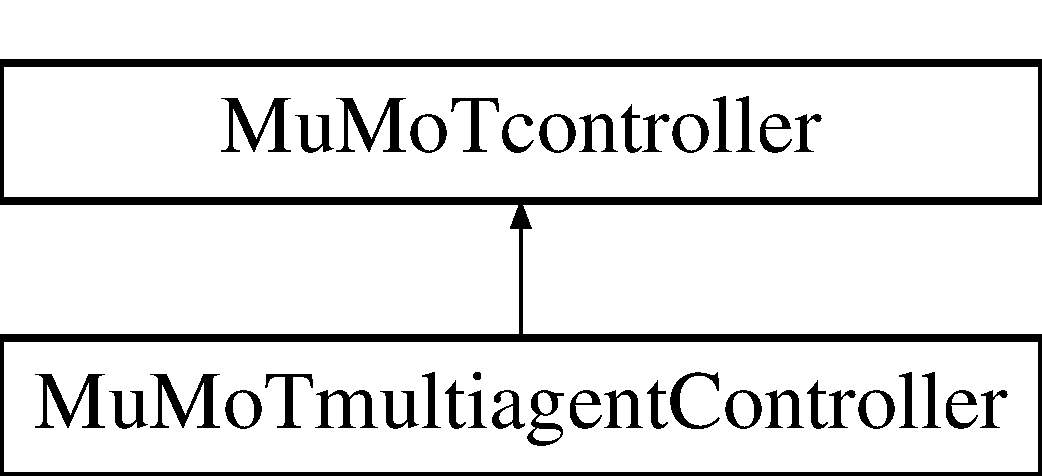
\includegraphics[height=2.000000cm]{class_mu_mo_t_1_1_mu_mo_t_1_1_mu_mo_tmultiagent_controller}
\end{center}
\end{figure}
\subsection*{Public Member Functions}
\begin{DoxyCompactItemize}
\item 
def \hyperlink{class_mu_mo_t_1_1_mu_mo_t_1_1_mu_mo_tmultiagent_controller_a819b06d2efbd452268cf86921dee8a43}{\+\_\+\+\_\+init\+\_\+\+\_\+} (self, param\+Values, param\+Names, param\+Label\+Dict, continuous\+Replot, M\+A\+Params, kwargs)
\item 
def \hyperlink{class_mu_mo_t_1_1_mu_mo_t_1_1_mu_mo_tmultiagent_controller_afa43c0f74ab5a6630a4b7ab0af8ed990}{download\+Time\+Evolution} (self)
\end{DoxyCompactItemize}
\subsection*{Private Member Functions}
\begin{DoxyCompactItemize}
\item 
def \hyperlink{class_mu_mo_t_1_1_mu_mo_t_1_1_mu_mo_tmultiagent_controller_a05f01fc433f3ff6861ec56d6663cb84e}{\+\_\+update\+\_\+net\+\_\+params} (self)
\end{DoxyCompactItemize}
\subsection*{Private Attributes}
\begin{DoxyCompactItemize}
\item 
\hyperlink{class_mu_mo_t_1_1_mu_mo_t_1_1_mu_mo_tmultiagent_controller_a018864aa22d2adb0d3958fb0adbce8e2}{\+\_\+progress\+Bar}
\begin{DoxyCompactList}\small\item\em Network type dropdown selector. \end{DoxyCompactList}\end{DoxyCompactItemize}


\subsection{Detailed Description}
class describing a controller for multiagent views 

\subsection{Constructor \& Destructor Documentation}
\mbox{\Hypertarget{class_mu_mo_t_1_1_mu_mo_t_1_1_mu_mo_tmultiagent_controller_a819b06d2efbd452268cf86921dee8a43}\label{class_mu_mo_t_1_1_mu_mo_t_1_1_mu_mo_tmultiagent_controller_a819b06d2efbd452268cf86921dee8a43}} 
\index{Mu\+Mo\+T\+::\+Mu\+Mo\+T\+::\+Mu\+Mo\+Tmultiagent\+Controller@{Mu\+Mo\+T\+::\+Mu\+Mo\+T\+::\+Mu\+Mo\+Tmultiagent\+Controller}!\+\_\+\+\_\+init\+\_\+\+\_\+@{\+\_\+\+\_\+init\+\_\+\+\_\+}}
\index{\+\_\+\+\_\+init\+\_\+\+\_\+@{\+\_\+\+\_\+init\+\_\+\+\_\+}!Mu\+Mo\+T\+::\+Mu\+Mo\+T\+::\+Mu\+Mo\+Tmultiagent\+Controller@{Mu\+Mo\+T\+::\+Mu\+Mo\+T\+::\+Mu\+Mo\+Tmultiagent\+Controller}}
\subsubsection{\texorpdfstring{\+\_\+\+\_\+init\+\_\+\+\_\+()}{\_\_init\_\_()}}
{\footnotesize\ttfamily def \+\_\+\+\_\+init\+\_\+\+\_\+ (\begin{DoxyParamCaption}\item[{}]{self,  }\item[{}]{param\+Values,  }\item[{}]{param\+Names,  }\item[{}]{param\+Label\+Dict,  }\item[{}]{continuous\+Replot,  }\item[{}]{M\+A\+Params,  }\item[{}]{kwargs }\end{DoxyParamCaption})}



\subsection{Member Function Documentation}
\mbox{\Hypertarget{class_mu_mo_t_1_1_mu_mo_t_1_1_mu_mo_tmultiagent_controller_a05f01fc433f3ff6861ec56d6663cb84e}\label{class_mu_mo_t_1_1_mu_mo_t_1_1_mu_mo_tmultiagent_controller_a05f01fc433f3ff6861ec56d6663cb84e}} 
\index{Mu\+Mo\+T\+::\+Mu\+Mo\+T\+::\+Mu\+Mo\+Tmultiagent\+Controller@{Mu\+Mo\+T\+::\+Mu\+Mo\+T\+::\+Mu\+Mo\+Tmultiagent\+Controller}!\+\_\+update\+\_\+net\+\_\+params@{\+\_\+update\+\_\+net\+\_\+params}}
\index{\+\_\+update\+\_\+net\+\_\+params@{\+\_\+update\+\_\+net\+\_\+params}!Mu\+Mo\+T\+::\+Mu\+Mo\+T\+::\+Mu\+Mo\+Tmultiagent\+Controller@{Mu\+Mo\+T\+::\+Mu\+Mo\+T\+::\+Mu\+Mo\+Tmultiagent\+Controller}}
\subsubsection{\texorpdfstring{\+\_\+update\+\_\+net\+\_\+params()}{\_update\_net\_params()}}
{\footnotesize\ttfamily def \+\_\+update\+\_\+net\+\_\+params (\begin{DoxyParamCaption}\item[{}]{self }\end{DoxyParamCaption})\hspace{0.3cm}{\ttfamily [private]}}

\mbox{\Hypertarget{class_mu_mo_t_1_1_mu_mo_t_1_1_mu_mo_tmultiagent_controller_afa43c0f74ab5a6630a4b7ab0af8ed990}\label{class_mu_mo_t_1_1_mu_mo_t_1_1_mu_mo_tmultiagent_controller_afa43c0f74ab5a6630a4b7ab0af8ed990}} 
\index{Mu\+Mo\+T\+::\+Mu\+Mo\+T\+::\+Mu\+Mo\+Tmultiagent\+Controller@{Mu\+Mo\+T\+::\+Mu\+Mo\+T\+::\+Mu\+Mo\+Tmultiagent\+Controller}!download\+Time\+Evolution@{download\+Time\+Evolution}}
\index{download\+Time\+Evolution@{download\+Time\+Evolution}!Mu\+Mo\+T\+::\+Mu\+Mo\+T\+::\+Mu\+Mo\+Tmultiagent\+Controller@{Mu\+Mo\+T\+::\+Mu\+Mo\+T\+::\+Mu\+Mo\+Tmultiagent\+Controller}}
\subsubsection{\texorpdfstring{download\+Time\+Evolution()}{downloadTimeEvolution()}}
{\footnotesize\ttfamily def download\+Time\+Evolution (\begin{DoxyParamCaption}\item[{}]{self }\end{DoxyParamCaption})}



\subsection{Field Documentation}
\mbox{\Hypertarget{class_mu_mo_t_1_1_mu_mo_t_1_1_mu_mo_tmultiagent_controller_a018864aa22d2adb0d3958fb0adbce8e2}\label{class_mu_mo_t_1_1_mu_mo_t_1_1_mu_mo_tmultiagent_controller_a018864aa22d2adb0d3958fb0adbce8e2}} 
\index{Mu\+Mo\+T\+::\+Mu\+Mo\+T\+::\+Mu\+Mo\+Tmultiagent\+Controller@{Mu\+Mo\+T\+::\+Mu\+Mo\+T\+::\+Mu\+Mo\+Tmultiagent\+Controller}!\+\_\+progress\+Bar@{\+\_\+progress\+Bar}}
\index{\+\_\+progress\+Bar@{\+\_\+progress\+Bar}!Mu\+Mo\+T\+::\+Mu\+Mo\+T\+::\+Mu\+Mo\+Tmultiagent\+Controller@{Mu\+Mo\+T\+::\+Mu\+Mo\+T\+::\+Mu\+Mo\+Tmultiagent\+Controller}}
\subsubsection{\texorpdfstring{\+\_\+progress\+Bar}{\_progressBar}}
{\footnotesize\ttfamily \+\_\+progress\+Bar\hspace{0.3cm}{\ttfamily [private]}}



Network type dropdown selector. 

\begin{DoxyRefDesc}{Todo}
\item[\hyperlink{todo__todo000024}{Todo}]\+: add network topology generated by random points in space \end{DoxyRefDesc}
Toggle buttons for plotting style 

The documentation for this class was generated from the following file\+:\begin{DoxyCompactItemize}
\item 
Mu\+Mo\+T/\hyperlink{_mu_mo_t_8py}{Mu\+Mo\+T.\+py}\end{DoxyCompactItemize}

\hypertarget{class_mu_mo_t_1_1_mu_mo_t_1_1_mu_mo_tmultiagent_view}{}\section{Mu\+Mo\+Tmultiagent\+View Class Reference}
\label{class_mu_mo_t_1_1_mu_mo_t_1_1_mu_mo_tmultiagent_view}\index{Mu\+Mo\+Tmultiagent\+View@{Mu\+Mo\+Tmultiagent\+View}}


agent on networks view on model  


Inheritance diagram for Mu\+Mo\+Tmultiagent\+View\+:\begin{figure}[H]
\begin{center}
\leavevmode
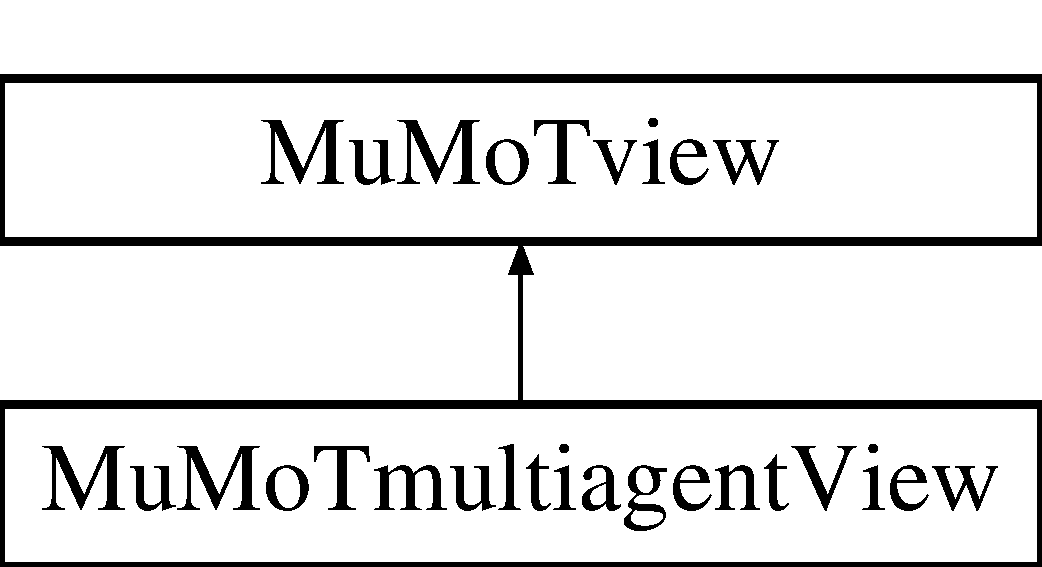
\includegraphics[height=2.000000cm]{class_mu_mo_t_1_1_mu_mo_t_1_1_mu_mo_tmultiagent_view}
\end{center}
\end{figure}
\subsection*{Public Member Functions}
\begin{DoxyCompactItemize}
\item 
def \hyperlink{class_mu_mo_t_1_1_mu_mo_t_1_1_mu_mo_tmultiagent_view_a3245dc2f896377d0265400e8181e7502}{\+\_\+\+\_\+init\+\_\+\+\_\+} (self, model, controller, M\+A\+Params, figure=None, rates=None, kwargs)
\end{DoxyCompactItemize}
\subsection*{Private Member Functions}
\begin{DoxyCompactItemize}
\item 
def \hyperlink{class_mu_mo_t_1_1_mu_mo_t_1_1_mu_mo_tmultiagent_view_a3af54c33f997937b14f422e772d5280a}{\+\_\+print\+\_\+standalone\+\_\+view\+\_\+cmd} (self)
\item 
def \hyperlink{class_mu_mo_t_1_1_mu_mo_t_1_1_mu_mo_tmultiagent_view_a47b00aaebcccf3c8dc2183a406404349}{\+\_\+update\+\_\+params} (self)
\begin{DoxyCompactList}\small\item\em reads the new parameters (in case they changed in the controller) this function should only update local parameters and not compute data \end{DoxyCompactList}\item 
def \hyperlink{class_mu_mo_t_1_1_mu_mo_t_1_1_mu_mo_tmultiagent_view_ace35072dcd3e51e67107f62b4de0d5fe}{\+\_\+plot\+\_\+time\+Evolution} (self)
\item 
def \hyperlink{class_mu_mo_t_1_1_mu_mo_t_1_1_mu_mo_tmultiagent_view_a57cea7fd9ea5c1805b9c18fc4b0adc0b}{\+\_\+redraw\+Only} (self)
\item 
def \hyperlink{class_mu_mo_t_1_1_mu_mo_t_1_1_mu_mo_tmultiagent_view_a62eb4d7a110764c65c992b5508540535}{\+\_\+run\+Multiagent} (self)
\item 
def \hyperlink{class_mu_mo_t_1_1_mu_mo_t_1_1_mu_mo_tmultiagent_view_a054aa0e8c130babbca21a6ff0e0fd31a}{\+\_\+init\+Figure} (self)
\item 
def \hyperlink{class_mu_mo_t_1_1_mu_mo_t_1_1_mu_mo_tmultiagent_view_a62d65f09387ea7930e7e2567edd23a9d}{\+\_\+update\+Multiagent\+Figure} (self, i, evo, position\+History, pos\+\_\+layout)
\item 
def \hyperlink{class_mu_mo_t_1_1_mu_mo_t_1_1_mu_mo_tmultiagent_view_a51d421aacb4cd83af5f1c2e60c3dff9c}{\+\_\+single\+Run} (self, random\+Seed)
\item 
def \hyperlink{class_mu_mo_t_1_1_mu_mo_t_1_1_mu_mo_tmultiagent_view_a63242960a1d4db3a17cc8657a8ee7da1}{\+\_\+convert\+Rates\+Into\+Probabilities} (self, reactants, rules)
\item 
def \hyperlink{class_mu_mo_t_1_1_mu_mo_t_1_1_mu_mo_tmultiagent_view_ad360a89687fc9a0298c853d76b8b8d95}{\+\_\+init\+Probabilities\+Map} (self, reactants, rules)
\begin{DoxyCompactList}\small\item\em derive the transition probabilities map from reaction rules \end{DoxyCompactList}\item 
def \hyperlink{class_mu_mo_t_1_1_mu_mo_t_1_1_mu_mo_tmultiagent_view_a064b5783c9e87092a7059fb632b56585}{\+\_\+compute\+Scaling\+Factor} (self)
\item 
def \hyperlink{class_mu_mo_t_1_1_mu_mo_t_1_1_mu_mo_tmultiagent_view_a5e541babe7e44e6888eb0ba92460cae2}{\+\_\+update\+\_\+timestep\+Size\+\_\+widget} (self, timestep\+Size)
\item 
def \hyperlink{class_mu_mo_t_1_1_mu_mo_t_1_1_mu_mo_tmultiagent_view_acc41eb1ddfc93fea7e67aa85c9d7f6fc}{\+\_\+apply\+Scaling\+Factor} (self)
\item 
def \hyperlink{class_mu_mo_t_1_1_mu_mo_t_1_1_mu_mo_tmultiagent_view_a0d226d5fb0e02291c96e1ff63a08047e}{\+\_\+init\+Graph} (self, graph\+Type, num\+Nodes, net\+Param=None)
\item 
def \hyperlink{class_mu_mo_t_1_1_mu_mo_t_1_1_mu_mo_tmultiagent_view_a4b9b689b183e0a18c7f60e48b6beafef}{\+\_\+init\+Multiagent} (self)
\item 
def \hyperlink{class_mu_mo_t_1_1_mu_mo_t_1_1_mu_mo_tmultiagent_view_a80b7d1f8c2f44ea9f4154b79f0baacfb}{\+\_\+step\+Multiagent} (self)
\item 
def \hyperlink{class_mu_mo_t_1_1_mu_mo_t_1_1_mu_mo_tmultiagent_view_a87f5913cd055f8e4eaa70b058ad7d77b}{\+\_\+step\+One\+Agent} (self, agent, neighs)
\begin{DoxyCompactList}\small\item\em one timestep for one agent \end{DoxyCompactList}\item 
def \hyperlink{class_mu_mo_t_1_1_mu_mo_t_1_1_mu_mo_tmultiagent_view_aba4da96cc2e7682af895cda4b1310790}{\+\_\+update\+Position} (self, x, y, o, speed, correlatedness)
\item 
def \hyperlink{class_mu_mo_t_1_1_mu_mo_t_1_1_mu_mo_tmultiagent_view_ad3df4b96d9dec10c8b806eb6697c6028}{\+\_\+get\+Neighbours} (self, agent, positions, distance\+\_\+range)
\begin{DoxyCompactList}\small\item\em return the (index) list of neighbours of \textquotesingle{}agent\textquotesingle{} \end{DoxyCompactList}\item 
def \hyperlink{class_mu_mo_t_1_1_mu_mo_t_1_1_mu_mo_tmultiagent_view_aa88fd0656cfcc7c9671c2bcc61d7726e}{\+\_\+distance\+\_\+on\+\_\+torus} (self, x\+\_\+1, y\+\_\+1, x\+\_\+2, y\+\_\+2)
\begin{DoxyCompactList}\small\item\em returns the minimum distance calucalted on the torus given by periodic boundary conditions \end{DoxyCompactList}\end{DoxyCompactItemize}
\subsection*{Private Attributes}
\begin{DoxyCompactItemize}
\item 
\hyperlink{class_mu_mo_t_1_1_mu_mo_t_1_1_mu_mo_tmultiagent_view_a15f56ca9811d1e67d721fa64f9b0dc1e}{\+\_\+controller}
\end{DoxyCompactItemize}
\subsection*{Static Private Attributes}
\begin{DoxyCompactItemize}
\item 
\hyperlink{class_mu_mo_t_1_1_mu_mo_t_1_1_mu_mo_tmultiagent_view_a6aaed74c935ed5380691798f75527a18}{\+\_\+colors} = None
\item 
\hyperlink{class_mu_mo_t_1_1_mu_mo_t_1_1_mu_mo_tmultiagent_view_aaf2c34c5022e4e3c872dbee11e50ea9b}{\+\_\+probabilities} = None
\item 
\hyperlink{class_mu_mo_t_1_1_mu_mo_t_1_1_mu_mo_tmultiagent_view_a752f43042d51a40fed348b434aad0fd8}{\+\_\+graph} = None
\begin{DoxyCompactList}\small\item\em structure to store the communication network \end{DoxyCompactList}\item 
\hyperlink{class_mu_mo_t_1_1_mu_mo_t_1_1_mu_mo_tmultiagent_view_a7d10cd5e301b167444880f57705e2b9e}{\+\_\+net\+Type} = None
\begin{DoxyCompactList}\small\item\em type of network used in the M-\/A simulation \end{DoxyCompactList}\item 
\hyperlink{class_mu_mo_t_1_1_mu_mo_t_1_1_mu_mo_tmultiagent_view_a187bc5499c4da612a9290851be253050}{\+\_\+net\+Param} = None
\begin{DoxyCompactList}\small\item\em network parameter which varies with respect to each type of network (for Erdos-\/\+Renyi is linking probability, for Barabasi-\/\+Albert is the number of edge per new node, for spatial is the communication range) \end{DoxyCompactList}\item 
\hyperlink{class_mu_mo_t_1_1_mu_mo_t_1_1_mu_mo_tmultiagent_view_a957e6b462fc11cb442a866d5b61367a0}{\+\_\+particle\+Speed} = None
\begin{DoxyCompactList}\small\item\em speed of the particle on one timestep (only for dynamic net\+Type) \end{DoxyCompactList}\item 
\hyperlink{class_mu_mo_t_1_1_mu_mo_t_1_1_mu_mo_tmultiagent_view_aa120ae2cb05f320428d90e34a49102ab}{\+\_\+motion\+Correlatedness} = None
\begin{DoxyCompactList}\small\item\em corelatedness in the random walk motion (only for dynamic net\+Type) \end{DoxyCompactList}\item 
\hyperlink{class_mu_mo_t_1_1_mu_mo_t_1_1_mu_mo_tmultiagent_view_a5032de31aad9de4528138249999e7d5f}{\+\_\+agents} = None
\begin{DoxyCompactList}\small\item\em list of agents involved in the simulation \end{DoxyCompactList}\item 
\hyperlink{class_mu_mo_t_1_1_mu_mo_t_1_1_mu_mo_tmultiagent_view_a8be9986760a86837e04718906d18d596}{\+\_\+positions} = None
\begin{DoxyCompactList}\small\item\em list of agents\textquotesingle{} positions \end{DoxyCompactList}\item 
int \hyperlink{class_mu_mo_t_1_1_mu_mo_t_1_1_mu_mo_tmultiagent_view_a372c083f5428e7f8a68298ec9dcca941}{\+\_\+arena\+\_\+width} = 1
\begin{DoxyCompactList}\small\item\em Arena size\+: width. \end{DoxyCompactList}\item 
int \hyperlink{class_mu_mo_t_1_1_mu_mo_t_1_1_mu_mo_tmultiagent_view_a12711c70e125709b78f820722ba74d09}{\+\_\+arena\+\_\+height} = 1
\begin{DoxyCompactList}\small\item\em Arena size\+: height. \end{DoxyCompactList}\item 
\hyperlink{class_mu_mo_t_1_1_mu_mo_t_1_1_mu_mo_tmultiagent_view_a8afeb8cf5705c6b521f7d6658dab955b}{\+\_\+initial\+State} = None
\begin{DoxyCompactList}\small\item\em the system state at the start of the simulation (timestep zero) \end{DoxyCompactList}\item 
\hyperlink{class_mu_mo_t_1_1_mu_mo_t_1_1_mu_mo_tmultiagent_view_a79e90c970112c845893400f85a2590dd}{\+\_\+random\+Seed} = None
\begin{DoxyCompactList}\small\item\em random seed \end{DoxyCompactList}\item 
\hyperlink{class_mu_mo_t_1_1_mu_mo_t_1_1_mu_mo_tmultiagent_view_a956572b83e957005ef90a30995891585}{\+\_\+max\+Time} = None
\begin{DoxyCompactList}\small\item\em number of simulation timesteps \end{DoxyCompactList}\item 
\hyperlink{class_mu_mo_t_1_1_mu_mo_t_1_1_mu_mo_tmultiagent_view_ad87100e87c83f6311376fa905bb9f579}{\+\_\+timestep\+Size} = None
\begin{DoxyCompactList}\small\item\em time scaling (i.\+e. \end{DoxyCompactList}\item 
\hyperlink{class_mu_mo_t_1_1_mu_mo_t_1_1_mu_mo_tmultiagent_view_a7c4303b3e2a8784a0cc16cd523069203}{\+\_\+rates\+Dict} = None
\begin{DoxyCompactList}\small\item\em dictionary of rates \end{DoxyCompactList}\item 
\hyperlink{class_mu_mo_t_1_1_mu_mo_t_1_1_mu_mo_tmultiagent_view_ae8c8d7969b8ab8f31df9d1d1d10eabb9}{\+\_\+visualisation\+Type} = None
\begin{DoxyCompactList}\small\item\em visualisation type \end{DoxyCompactList}\item 
\hyperlink{class_mu_mo_t_1_1_mu_mo_t_1_1_mu_mo_tmultiagent_view_a756f7d76f2b84a0dd60ffd6b7683dd3a}{\+\_\+show\+Trace} = None
\begin{DoxyCompactList}\small\item\em visualise the agent trace (on moving particles) \end{DoxyCompactList}\item 
\hyperlink{class_mu_mo_t_1_1_mu_mo_t_1_1_mu_mo_tmultiagent_view_ad3f953eaa70c3e4eee2dde80e57c638f}{\+\_\+show\+Interactions} = None
\begin{DoxyCompactList}\small\item\em visualise the agent trace (on moving particles) \end{DoxyCompactList}\item 
\hyperlink{class_mu_mo_t_1_1_mu_mo_t_1_1_mu_mo_tmultiagent_view_a194d04e5fee40987d78aa7e1f721ea28}{\+\_\+realtime\+Plot} = None
\begin{DoxyCompactList}\small\item\em realtime\+Plot flag (T\+R\+UE = the plot is updated each timestep of the simulation; F\+A\+L\+SE = it is updated once at the end of the simulation) \end{DoxyCompactList}\item 
\hyperlink{class_mu_mo_t_1_1_mu_mo_t_1_1_mu_mo_tmultiagent_view_a8da8c49a2b0ccc518cf7f333bdbd17a6}{\+\_\+latest\+Results} = None
\begin{DoxyCompactList}\small\item\em latest computed results \end{DoxyCompactList}\end{DoxyCompactItemize}
\subsection*{Additional Inherited Members}


\subsection{Detailed Description}
agent on networks view on model 

\subsection{Constructor \& Destructor Documentation}
\mbox{\Hypertarget{class_mu_mo_t_1_1_mu_mo_t_1_1_mu_mo_tmultiagent_view_a3245dc2f896377d0265400e8181e7502}\label{class_mu_mo_t_1_1_mu_mo_t_1_1_mu_mo_tmultiagent_view_a3245dc2f896377d0265400e8181e7502}} 
\index{Mu\+Mo\+T\+::\+Mu\+Mo\+T\+::\+Mu\+Mo\+Tmultiagent\+View@{Mu\+Mo\+T\+::\+Mu\+Mo\+T\+::\+Mu\+Mo\+Tmultiagent\+View}!\+\_\+\+\_\+init\+\_\+\+\_\+@{\+\_\+\+\_\+init\+\_\+\+\_\+}}
\index{\+\_\+\+\_\+init\+\_\+\+\_\+@{\+\_\+\+\_\+init\+\_\+\+\_\+}!Mu\+Mo\+T\+::\+Mu\+Mo\+T\+::\+Mu\+Mo\+Tmultiagent\+View@{Mu\+Mo\+T\+::\+Mu\+Mo\+T\+::\+Mu\+Mo\+Tmultiagent\+View}}
\subsubsection{\texorpdfstring{\+\_\+\+\_\+init\+\_\+\+\_\+()}{\_\_init\_\_()}}
{\footnotesize\ttfamily def \+\_\+\+\_\+init\+\_\+\+\_\+ (\begin{DoxyParamCaption}\item[{}]{self,  }\item[{}]{model,  }\item[{}]{controller,  }\item[{}]{M\+A\+Params,  }\item[{}]{figure = {\ttfamily None},  }\item[{}]{rates = {\ttfamily None},  }\item[{}]{kwargs }\end{DoxyParamCaption})}



\subsection{Member Function Documentation}
\mbox{\Hypertarget{class_mu_mo_t_1_1_mu_mo_t_1_1_mu_mo_tmultiagent_view_acc41eb1ddfc93fea7e67aa85c9d7f6fc}\label{class_mu_mo_t_1_1_mu_mo_t_1_1_mu_mo_tmultiagent_view_acc41eb1ddfc93fea7e67aa85c9d7f6fc}} 
\index{Mu\+Mo\+T\+::\+Mu\+Mo\+T\+::\+Mu\+Mo\+Tmultiagent\+View@{Mu\+Mo\+T\+::\+Mu\+Mo\+T\+::\+Mu\+Mo\+Tmultiagent\+View}!\+\_\+apply\+Scaling\+Factor@{\+\_\+apply\+Scaling\+Factor}}
\index{\+\_\+apply\+Scaling\+Factor@{\+\_\+apply\+Scaling\+Factor}!Mu\+Mo\+T\+::\+Mu\+Mo\+T\+::\+Mu\+Mo\+Tmultiagent\+View@{Mu\+Mo\+T\+::\+Mu\+Mo\+T\+::\+Mu\+Mo\+Tmultiagent\+View}}
\subsubsection{\texorpdfstring{\+\_\+apply\+Scaling\+Factor()}{\_applyScalingFactor()}}
{\footnotesize\ttfamily def \+\_\+apply\+Scaling\+Factor (\begin{DoxyParamCaption}\item[{}]{self }\end{DoxyParamCaption})\hspace{0.3cm}{\ttfamily [private]}}

\mbox{\Hypertarget{class_mu_mo_t_1_1_mu_mo_t_1_1_mu_mo_tmultiagent_view_a064b5783c9e87092a7059fb632b56585}\label{class_mu_mo_t_1_1_mu_mo_t_1_1_mu_mo_tmultiagent_view_a064b5783c9e87092a7059fb632b56585}} 
\index{Mu\+Mo\+T\+::\+Mu\+Mo\+T\+::\+Mu\+Mo\+Tmultiagent\+View@{Mu\+Mo\+T\+::\+Mu\+Mo\+T\+::\+Mu\+Mo\+Tmultiagent\+View}!\+\_\+compute\+Scaling\+Factor@{\+\_\+compute\+Scaling\+Factor}}
\index{\+\_\+compute\+Scaling\+Factor@{\+\_\+compute\+Scaling\+Factor}!Mu\+Mo\+T\+::\+Mu\+Mo\+T\+::\+Mu\+Mo\+Tmultiagent\+View@{Mu\+Mo\+T\+::\+Mu\+Mo\+T\+::\+Mu\+Mo\+Tmultiagent\+View}}
\subsubsection{\texorpdfstring{\+\_\+compute\+Scaling\+Factor()}{\_computeScalingFactor()}}
{\footnotesize\ttfamily def \+\_\+compute\+Scaling\+Factor (\begin{DoxyParamCaption}\item[{}]{self }\end{DoxyParamCaption})\hspace{0.3cm}{\ttfamily [private]}}

\mbox{\Hypertarget{class_mu_mo_t_1_1_mu_mo_t_1_1_mu_mo_tmultiagent_view_a63242960a1d4db3a17cc8657a8ee7da1}\label{class_mu_mo_t_1_1_mu_mo_t_1_1_mu_mo_tmultiagent_view_a63242960a1d4db3a17cc8657a8ee7da1}} 
\index{Mu\+Mo\+T\+::\+Mu\+Mo\+T\+::\+Mu\+Mo\+Tmultiagent\+View@{Mu\+Mo\+T\+::\+Mu\+Mo\+T\+::\+Mu\+Mo\+Tmultiagent\+View}!\+\_\+convert\+Rates\+Into\+Probabilities@{\+\_\+convert\+Rates\+Into\+Probabilities}}
\index{\+\_\+convert\+Rates\+Into\+Probabilities@{\+\_\+convert\+Rates\+Into\+Probabilities}!Mu\+Mo\+T\+::\+Mu\+Mo\+T\+::\+Mu\+Mo\+Tmultiagent\+View@{Mu\+Mo\+T\+::\+Mu\+Mo\+T\+::\+Mu\+Mo\+Tmultiagent\+View}}
\subsubsection{\texorpdfstring{\+\_\+convert\+Rates\+Into\+Probabilities()}{\_convertRatesIntoProbabilities()}}
{\footnotesize\ttfamily def \+\_\+convert\+Rates\+Into\+Probabilities (\begin{DoxyParamCaption}\item[{}]{self,  }\item[{}]{reactants,  }\item[{}]{rules }\end{DoxyParamCaption})\hspace{0.3cm}{\ttfamily [private]}}

\mbox{\Hypertarget{class_mu_mo_t_1_1_mu_mo_t_1_1_mu_mo_tmultiagent_view_aa88fd0656cfcc7c9671c2bcc61d7726e}\label{class_mu_mo_t_1_1_mu_mo_t_1_1_mu_mo_tmultiagent_view_aa88fd0656cfcc7c9671c2bcc61d7726e}} 
\index{Mu\+Mo\+T\+::\+Mu\+Mo\+T\+::\+Mu\+Mo\+Tmultiagent\+View@{Mu\+Mo\+T\+::\+Mu\+Mo\+T\+::\+Mu\+Mo\+Tmultiagent\+View}!\+\_\+distance\+\_\+on\+\_\+torus@{\+\_\+distance\+\_\+on\+\_\+torus}}
\index{\+\_\+distance\+\_\+on\+\_\+torus@{\+\_\+distance\+\_\+on\+\_\+torus}!Mu\+Mo\+T\+::\+Mu\+Mo\+T\+::\+Mu\+Mo\+Tmultiagent\+View@{Mu\+Mo\+T\+::\+Mu\+Mo\+T\+::\+Mu\+Mo\+Tmultiagent\+View}}
\subsubsection{\texorpdfstring{\+\_\+distance\+\_\+on\+\_\+torus()}{\_distance\_on\_torus()}}
{\footnotesize\ttfamily def \+\_\+distance\+\_\+on\+\_\+torus (\begin{DoxyParamCaption}\item[{}]{self,  }\item[{}]{x\+\_\+1,  }\item[{}]{y\+\_\+1,  }\item[{}]{x\+\_\+2,  }\item[{}]{y\+\_\+2 }\end{DoxyParamCaption})\hspace{0.3cm}{\ttfamily [private]}}



returns the minimum distance calucalted on the torus given by periodic boundary conditions 

\mbox{\Hypertarget{class_mu_mo_t_1_1_mu_mo_t_1_1_mu_mo_tmultiagent_view_ad3df4b96d9dec10c8b806eb6697c6028}\label{class_mu_mo_t_1_1_mu_mo_t_1_1_mu_mo_tmultiagent_view_ad3df4b96d9dec10c8b806eb6697c6028}} 
\index{Mu\+Mo\+T\+::\+Mu\+Mo\+T\+::\+Mu\+Mo\+Tmultiagent\+View@{Mu\+Mo\+T\+::\+Mu\+Mo\+T\+::\+Mu\+Mo\+Tmultiagent\+View}!\+\_\+get\+Neighbours@{\+\_\+get\+Neighbours}}
\index{\+\_\+get\+Neighbours@{\+\_\+get\+Neighbours}!Mu\+Mo\+T\+::\+Mu\+Mo\+T\+::\+Mu\+Mo\+Tmultiagent\+View@{Mu\+Mo\+T\+::\+Mu\+Mo\+T\+::\+Mu\+Mo\+Tmultiagent\+View}}
\subsubsection{\texorpdfstring{\+\_\+get\+Neighbours()}{\_getNeighbours()}}
{\footnotesize\ttfamily def \+\_\+get\+Neighbours (\begin{DoxyParamCaption}\item[{}]{self,  }\item[{}]{agent,  }\item[{}]{positions,  }\item[{}]{distance\+\_\+range }\end{DoxyParamCaption})\hspace{0.3cm}{\ttfamily [private]}}



return the (index) list of neighbours of \textquotesingle{}agent\textquotesingle{} 

\mbox{\Hypertarget{class_mu_mo_t_1_1_mu_mo_t_1_1_mu_mo_tmultiagent_view_a054aa0e8c130babbca21a6ff0e0fd31a}\label{class_mu_mo_t_1_1_mu_mo_t_1_1_mu_mo_tmultiagent_view_a054aa0e8c130babbca21a6ff0e0fd31a}} 
\index{Mu\+Mo\+T\+::\+Mu\+Mo\+T\+::\+Mu\+Mo\+Tmultiagent\+View@{Mu\+Mo\+T\+::\+Mu\+Mo\+T\+::\+Mu\+Mo\+Tmultiagent\+View}!\+\_\+init\+Figure@{\+\_\+init\+Figure}}
\index{\+\_\+init\+Figure@{\+\_\+init\+Figure}!Mu\+Mo\+T\+::\+Mu\+Mo\+T\+::\+Mu\+Mo\+Tmultiagent\+View@{Mu\+Mo\+T\+::\+Mu\+Mo\+T\+::\+Mu\+Mo\+Tmultiagent\+View}}
\subsubsection{\texorpdfstring{\+\_\+init\+Figure()}{\_initFigure()}}
{\footnotesize\ttfamily def \+\_\+init\+Figure (\begin{DoxyParamCaption}\item[{}]{self }\end{DoxyParamCaption})\hspace{0.3cm}{\ttfamily [private]}}

\mbox{\Hypertarget{class_mu_mo_t_1_1_mu_mo_t_1_1_mu_mo_tmultiagent_view_a0d226d5fb0e02291c96e1ff63a08047e}\label{class_mu_mo_t_1_1_mu_mo_t_1_1_mu_mo_tmultiagent_view_a0d226d5fb0e02291c96e1ff63a08047e}} 
\index{Mu\+Mo\+T\+::\+Mu\+Mo\+T\+::\+Mu\+Mo\+Tmultiagent\+View@{Mu\+Mo\+T\+::\+Mu\+Mo\+T\+::\+Mu\+Mo\+Tmultiagent\+View}!\+\_\+init\+Graph@{\+\_\+init\+Graph}}
\index{\+\_\+init\+Graph@{\+\_\+init\+Graph}!Mu\+Mo\+T\+::\+Mu\+Mo\+T\+::\+Mu\+Mo\+Tmultiagent\+View@{Mu\+Mo\+T\+::\+Mu\+Mo\+T\+::\+Mu\+Mo\+Tmultiagent\+View}}
\subsubsection{\texorpdfstring{\+\_\+init\+Graph()}{\_initGraph()}}
{\footnotesize\ttfamily def \+\_\+init\+Graph (\begin{DoxyParamCaption}\item[{}]{self,  }\item[{}]{graph\+Type,  }\item[{}]{num\+Nodes,  }\item[{}]{net\+Param = {\ttfamily None} }\end{DoxyParamCaption})\hspace{0.3cm}{\ttfamily [private]}}

\mbox{\Hypertarget{class_mu_mo_t_1_1_mu_mo_t_1_1_mu_mo_tmultiagent_view_a4b9b689b183e0a18c7f60e48b6beafef}\label{class_mu_mo_t_1_1_mu_mo_t_1_1_mu_mo_tmultiagent_view_a4b9b689b183e0a18c7f60e48b6beafef}} 
\index{Mu\+Mo\+T\+::\+Mu\+Mo\+T\+::\+Mu\+Mo\+Tmultiagent\+View@{Mu\+Mo\+T\+::\+Mu\+Mo\+T\+::\+Mu\+Mo\+Tmultiagent\+View}!\+\_\+init\+Multiagent@{\+\_\+init\+Multiagent}}
\index{\+\_\+init\+Multiagent@{\+\_\+init\+Multiagent}!Mu\+Mo\+T\+::\+Mu\+Mo\+T\+::\+Mu\+Mo\+Tmultiagent\+View@{Mu\+Mo\+T\+::\+Mu\+Mo\+T\+::\+Mu\+Mo\+Tmultiagent\+View}}
\subsubsection{\texorpdfstring{\+\_\+init\+Multiagent()}{\_initMultiagent()}}
{\footnotesize\ttfamily def \+\_\+init\+Multiagent (\begin{DoxyParamCaption}\item[{}]{self }\end{DoxyParamCaption})\hspace{0.3cm}{\ttfamily [private]}}

\mbox{\Hypertarget{class_mu_mo_t_1_1_mu_mo_t_1_1_mu_mo_tmultiagent_view_ad360a89687fc9a0298c853d76b8b8d95}\label{class_mu_mo_t_1_1_mu_mo_t_1_1_mu_mo_tmultiagent_view_ad360a89687fc9a0298c853d76b8b8d95}} 
\index{Mu\+Mo\+T\+::\+Mu\+Mo\+T\+::\+Mu\+Mo\+Tmultiagent\+View@{Mu\+Mo\+T\+::\+Mu\+Mo\+T\+::\+Mu\+Mo\+Tmultiagent\+View}!\+\_\+init\+Probabilities\+Map@{\+\_\+init\+Probabilities\+Map}}
\index{\+\_\+init\+Probabilities\+Map@{\+\_\+init\+Probabilities\+Map}!Mu\+Mo\+T\+::\+Mu\+Mo\+T\+::\+Mu\+Mo\+Tmultiagent\+View@{Mu\+Mo\+T\+::\+Mu\+Mo\+T\+::\+Mu\+Mo\+Tmultiagent\+View}}
\subsubsection{\texorpdfstring{\+\_\+init\+Probabilities\+Map()}{\_initProbabilitiesMap()}}
{\footnotesize\ttfamily def \+\_\+init\+Probabilities\+Map (\begin{DoxyParamCaption}\item[{}]{self,  }\item[{}]{reactants,  }\item[{}]{rules }\end{DoxyParamCaption})\hspace{0.3cm}{\ttfamily [private]}}



derive the transition probabilities map from reaction rules 

\mbox{\Hypertarget{class_mu_mo_t_1_1_mu_mo_t_1_1_mu_mo_tmultiagent_view_ace35072dcd3e51e67107f62b4de0d5fe}\label{class_mu_mo_t_1_1_mu_mo_t_1_1_mu_mo_tmultiagent_view_ace35072dcd3e51e67107f62b4de0d5fe}} 
\index{Mu\+Mo\+T\+::\+Mu\+Mo\+T\+::\+Mu\+Mo\+Tmultiagent\+View@{Mu\+Mo\+T\+::\+Mu\+Mo\+T\+::\+Mu\+Mo\+Tmultiagent\+View}!\+\_\+plot\+\_\+time\+Evolution@{\+\_\+plot\+\_\+time\+Evolution}}
\index{\+\_\+plot\+\_\+time\+Evolution@{\+\_\+plot\+\_\+time\+Evolution}!Mu\+Mo\+T\+::\+Mu\+Mo\+T\+::\+Mu\+Mo\+Tmultiagent\+View@{Mu\+Mo\+T\+::\+Mu\+Mo\+T\+::\+Mu\+Mo\+Tmultiagent\+View}}
\subsubsection{\texorpdfstring{\+\_\+plot\+\_\+time\+Evolution()}{\_plot\_timeEvolution()}}
{\footnotesize\ttfamily def \+\_\+plot\+\_\+time\+Evolution (\begin{DoxyParamCaption}\item[{}]{self }\end{DoxyParamCaption})\hspace{0.3cm}{\ttfamily [private]}}

\mbox{\Hypertarget{class_mu_mo_t_1_1_mu_mo_t_1_1_mu_mo_tmultiagent_view_a3af54c33f997937b14f422e772d5280a}\label{class_mu_mo_t_1_1_mu_mo_t_1_1_mu_mo_tmultiagent_view_a3af54c33f997937b14f422e772d5280a}} 
\index{Mu\+Mo\+T\+::\+Mu\+Mo\+T\+::\+Mu\+Mo\+Tmultiagent\+View@{Mu\+Mo\+T\+::\+Mu\+Mo\+T\+::\+Mu\+Mo\+Tmultiagent\+View}!\+\_\+print\+\_\+standalone\+\_\+view\+\_\+cmd@{\+\_\+print\+\_\+standalone\+\_\+view\+\_\+cmd}}
\index{\+\_\+print\+\_\+standalone\+\_\+view\+\_\+cmd@{\+\_\+print\+\_\+standalone\+\_\+view\+\_\+cmd}!Mu\+Mo\+T\+::\+Mu\+Mo\+T\+::\+Mu\+Mo\+Tmultiagent\+View@{Mu\+Mo\+T\+::\+Mu\+Mo\+T\+::\+Mu\+Mo\+Tmultiagent\+View}}
\subsubsection{\texorpdfstring{\+\_\+print\+\_\+standalone\+\_\+view\+\_\+cmd()}{\_print\_standalone\_view\_cmd()}}
{\footnotesize\ttfamily def \+\_\+print\+\_\+standalone\+\_\+view\+\_\+cmd (\begin{DoxyParamCaption}\item[{}]{self }\end{DoxyParamCaption})\hspace{0.3cm}{\ttfamily [private]}}

\mbox{\Hypertarget{class_mu_mo_t_1_1_mu_mo_t_1_1_mu_mo_tmultiagent_view_a57cea7fd9ea5c1805b9c18fc4b0adc0b}\label{class_mu_mo_t_1_1_mu_mo_t_1_1_mu_mo_tmultiagent_view_a57cea7fd9ea5c1805b9c18fc4b0adc0b}} 
\index{Mu\+Mo\+T\+::\+Mu\+Mo\+T\+::\+Mu\+Mo\+Tmultiagent\+View@{Mu\+Mo\+T\+::\+Mu\+Mo\+T\+::\+Mu\+Mo\+Tmultiagent\+View}!\+\_\+redraw\+Only@{\+\_\+redraw\+Only}}
\index{\+\_\+redraw\+Only@{\+\_\+redraw\+Only}!Mu\+Mo\+T\+::\+Mu\+Mo\+T\+::\+Mu\+Mo\+Tmultiagent\+View@{Mu\+Mo\+T\+::\+Mu\+Mo\+T\+::\+Mu\+Mo\+Tmultiagent\+View}}
\subsubsection{\texorpdfstring{\+\_\+redraw\+Only()}{\_redrawOnly()}}
{\footnotesize\ttfamily def \+\_\+redraw\+Only (\begin{DoxyParamCaption}\item[{}]{self }\end{DoxyParamCaption})\hspace{0.3cm}{\ttfamily [private]}}

\mbox{\Hypertarget{class_mu_mo_t_1_1_mu_mo_t_1_1_mu_mo_tmultiagent_view_a62eb4d7a110764c65c992b5508540535}\label{class_mu_mo_t_1_1_mu_mo_t_1_1_mu_mo_tmultiagent_view_a62eb4d7a110764c65c992b5508540535}} 
\index{Mu\+Mo\+T\+::\+Mu\+Mo\+T\+::\+Mu\+Mo\+Tmultiagent\+View@{Mu\+Mo\+T\+::\+Mu\+Mo\+T\+::\+Mu\+Mo\+Tmultiagent\+View}!\+\_\+run\+Multiagent@{\+\_\+run\+Multiagent}}
\index{\+\_\+run\+Multiagent@{\+\_\+run\+Multiagent}!Mu\+Mo\+T\+::\+Mu\+Mo\+T\+::\+Mu\+Mo\+Tmultiagent\+View@{Mu\+Mo\+T\+::\+Mu\+Mo\+T\+::\+Mu\+Mo\+Tmultiagent\+View}}
\subsubsection{\texorpdfstring{\+\_\+run\+Multiagent()}{\_runMultiagent()}}
{\footnotesize\ttfamily def \+\_\+run\+Multiagent (\begin{DoxyParamCaption}\item[{}]{self }\end{DoxyParamCaption})\hspace{0.3cm}{\ttfamily [private]}}

\mbox{\Hypertarget{class_mu_mo_t_1_1_mu_mo_t_1_1_mu_mo_tmultiagent_view_a51d421aacb4cd83af5f1c2e60c3dff9c}\label{class_mu_mo_t_1_1_mu_mo_t_1_1_mu_mo_tmultiagent_view_a51d421aacb4cd83af5f1c2e60c3dff9c}} 
\index{Mu\+Mo\+T\+::\+Mu\+Mo\+T\+::\+Mu\+Mo\+Tmultiagent\+View@{Mu\+Mo\+T\+::\+Mu\+Mo\+T\+::\+Mu\+Mo\+Tmultiagent\+View}!\+\_\+single\+Run@{\+\_\+single\+Run}}
\index{\+\_\+single\+Run@{\+\_\+single\+Run}!Mu\+Mo\+T\+::\+Mu\+Mo\+T\+::\+Mu\+Mo\+Tmultiagent\+View@{Mu\+Mo\+T\+::\+Mu\+Mo\+T\+::\+Mu\+Mo\+Tmultiagent\+View}}
\subsubsection{\texorpdfstring{\+\_\+single\+Run()}{\_singleRun()}}
{\footnotesize\ttfamily def \+\_\+single\+Run (\begin{DoxyParamCaption}\item[{}]{self,  }\item[{}]{random\+Seed }\end{DoxyParamCaption})\hspace{0.3cm}{\ttfamily [private]}}

\mbox{\Hypertarget{class_mu_mo_t_1_1_mu_mo_t_1_1_mu_mo_tmultiagent_view_a80b7d1f8c2f44ea9f4154b79f0baacfb}\label{class_mu_mo_t_1_1_mu_mo_t_1_1_mu_mo_tmultiagent_view_a80b7d1f8c2f44ea9f4154b79f0baacfb}} 
\index{Mu\+Mo\+T\+::\+Mu\+Mo\+T\+::\+Mu\+Mo\+Tmultiagent\+View@{Mu\+Mo\+T\+::\+Mu\+Mo\+T\+::\+Mu\+Mo\+Tmultiagent\+View}!\+\_\+step\+Multiagent@{\+\_\+step\+Multiagent}}
\index{\+\_\+step\+Multiagent@{\+\_\+step\+Multiagent}!Mu\+Mo\+T\+::\+Mu\+Mo\+T\+::\+Mu\+Mo\+Tmultiagent\+View@{Mu\+Mo\+T\+::\+Mu\+Mo\+T\+::\+Mu\+Mo\+Tmultiagent\+View}}
\subsubsection{\texorpdfstring{\+\_\+step\+Multiagent()}{\_stepMultiagent()}}
{\footnotesize\ttfamily def \+\_\+step\+Multiagent (\begin{DoxyParamCaption}\item[{}]{self }\end{DoxyParamCaption})\hspace{0.3cm}{\ttfamily [private]}}

\mbox{\Hypertarget{class_mu_mo_t_1_1_mu_mo_t_1_1_mu_mo_tmultiagent_view_a87f5913cd055f8e4eaa70b058ad7d77b}\label{class_mu_mo_t_1_1_mu_mo_t_1_1_mu_mo_tmultiagent_view_a87f5913cd055f8e4eaa70b058ad7d77b}} 
\index{Mu\+Mo\+T\+::\+Mu\+Mo\+T\+::\+Mu\+Mo\+Tmultiagent\+View@{Mu\+Mo\+T\+::\+Mu\+Mo\+T\+::\+Mu\+Mo\+Tmultiagent\+View}!\+\_\+step\+One\+Agent@{\+\_\+step\+One\+Agent}}
\index{\+\_\+step\+One\+Agent@{\+\_\+step\+One\+Agent}!Mu\+Mo\+T\+::\+Mu\+Mo\+T\+::\+Mu\+Mo\+Tmultiagent\+View@{Mu\+Mo\+T\+::\+Mu\+Mo\+T\+::\+Mu\+Mo\+Tmultiagent\+View}}
\subsubsection{\texorpdfstring{\+\_\+step\+One\+Agent()}{\_stepOneAgent()}}
{\footnotesize\ttfamily def \+\_\+step\+One\+Agent (\begin{DoxyParamCaption}\item[{}]{self,  }\item[{}]{agent,  }\item[{}]{neighs }\end{DoxyParamCaption})\hspace{0.3cm}{\ttfamily [private]}}



one timestep for one agent 

\mbox{\Hypertarget{class_mu_mo_t_1_1_mu_mo_t_1_1_mu_mo_tmultiagent_view_a47b00aaebcccf3c8dc2183a406404349}\label{class_mu_mo_t_1_1_mu_mo_t_1_1_mu_mo_tmultiagent_view_a47b00aaebcccf3c8dc2183a406404349}} 
\index{Mu\+Mo\+T\+::\+Mu\+Mo\+T\+::\+Mu\+Mo\+Tmultiagent\+View@{Mu\+Mo\+T\+::\+Mu\+Mo\+T\+::\+Mu\+Mo\+Tmultiagent\+View}!\+\_\+update\+\_\+params@{\+\_\+update\+\_\+params}}
\index{\+\_\+update\+\_\+params@{\+\_\+update\+\_\+params}!Mu\+Mo\+T\+::\+Mu\+Mo\+T\+::\+Mu\+Mo\+Tmultiagent\+View@{Mu\+Mo\+T\+::\+Mu\+Mo\+T\+::\+Mu\+Mo\+Tmultiagent\+View}}
\subsubsection{\texorpdfstring{\+\_\+update\+\_\+params()}{\_update\_params()}}
{\footnotesize\ttfamily def \+\_\+update\+\_\+params (\begin{DoxyParamCaption}\item[{}]{self }\end{DoxyParamCaption})\hspace{0.3cm}{\ttfamily [private]}}



reads the new parameters (in case they changed in the controller) this function should only update local parameters and not compute data 

\mbox{\Hypertarget{class_mu_mo_t_1_1_mu_mo_t_1_1_mu_mo_tmultiagent_view_a5e541babe7e44e6888eb0ba92460cae2}\label{class_mu_mo_t_1_1_mu_mo_t_1_1_mu_mo_tmultiagent_view_a5e541babe7e44e6888eb0ba92460cae2}} 
\index{Mu\+Mo\+T\+::\+Mu\+Mo\+T\+::\+Mu\+Mo\+Tmultiagent\+View@{Mu\+Mo\+T\+::\+Mu\+Mo\+T\+::\+Mu\+Mo\+Tmultiagent\+View}!\+\_\+update\+\_\+timestep\+Size\+\_\+widget@{\+\_\+update\+\_\+timestep\+Size\+\_\+widget}}
\index{\+\_\+update\+\_\+timestep\+Size\+\_\+widget@{\+\_\+update\+\_\+timestep\+Size\+\_\+widget}!Mu\+Mo\+T\+::\+Mu\+Mo\+T\+::\+Mu\+Mo\+Tmultiagent\+View@{Mu\+Mo\+T\+::\+Mu\+Mo\+T\+::\+Mu\+Mo\+Tmultiagent\+View}}
\subsubsection{\texorpdfstring{\+\_\+update\+\_\+timestep\+Size\+\_\+widget()}{\_update\_timestepSize\_widget()}}
{\footnotesize\ttfamily def \+\_\+update\+\_\+timestep\+Size\+\_\+widget (\begin{DoxyParamCaption}\item[{}]{self,  }\item[{}]{timestep\+Size }\end{DoxyParamCaption})\hspace{0.3cm}{\ttfamily [private]}}

\mbox{\Hypertarget{class_mu_mo_t_1_1_mu_mo_t_1_1_mu_mo_tmultiagent_view_a62d65f09387ea7930e7e2567edd23a9d}\label{class_mu_mo_t_1_1_mu_mo_t_1_1_mu_mo_tmultiagent_view_a62d65f09387ea7930e7e2567edd23a9d}} 
\index{Mu\+Mo\+T\+::\+Mu\+Mo\+T\+::\+Mu\+Mo\+Tmultiagent\+View@{Mu\+Mo\+T\+::\+Mu\+Mo\+T\+::\+Mu\+Mo\+Tmultiagent\+View}!\+\_\+update\+Multiagent\+Figure@{\+\_\+update\+Multiagent\+Figure}}
\index{\+\_\+update\+Multiagent\+Figure@{\+\_\+update\+Multiagent\+Figure}!Mu\+Mo\+T\+::\+Mu\+Mo\+T\+::\+Mu\+Mo\+Tmultiagent\+View@{Mu\+Mo\+T\+::\+Mu\+Mo\+T\+::\+Mu\+Mo\+Tmultiagent\+View}}
\subsubsection{\texorpdfstring{\+\_\+update\+Multiagent\+Figure()}{\_updateMultiagentFigure()}}
{\footnotesize\ttfamily def \+\_\+update\+Multiagent\+Figure (\begin{DoxyParamCaption}\item[{}]{self,  }\item[{}]{i,  }\item[{}]{evo,  }\item[{}]{position\+History,  }\item[{}]{pos\+\_\+layout }\end{DoxyParamCaption})\hspace{0.3cm}{\ttfamily [private]}}

\mbox{\Hypertarget{class_mu_mo_t_1_1_mu_mo_t_1_1_mu_mo_tmultiagent_view_aba4da96cc2e7682af895cda4b1310790}\label{class_mu_mo_t_1_1_mu_mo_t_1_1_mu_mo_tmultiagent_view_aba4da96cc2e7682af895cda4b1310790}} 
\index{Mu\+Mo\+T\+::\+Mu\+Mo\+T\+::\+Mu\+Mo\+Tmultiagent\+View@{Mu\+Mo\+T\+::\+Mu\+Mo\+T\+::\+Mu\+Mo\+Tmultiagent\+View}!\+\_\+update\+Position@{\+\_\+update\+Position}}
\index{\+\_\+update\+Position@{\+\_\+update\+Position}!Mu\+Mo\+T\+::\+Mu\+Mo\+T\+::\+Mu\+Mo\+Tmultiagent\+View@{Mu\+Mo\+T\+::\+Mu\+Mo\+T\+::\+Mu\+Mo\+Tmultiagent\+View}}
\subsubsection{\texorpdfstring{\+\_\+update\+Position()}{\_updatePosition()}}
{\footnotesize\ttfamily def \+\_\+update\+Position (\begin{DoxyParamCaption}\item[{}]{self,  }\item[{}]{x,  }\item[{}]{y,  }\item[{}]{o,  }\item[{}]{speed,  }\item[{}]{correlatedness }\end{DoxyParamCaption})\hspace{0.3cm}{\ttfamily [private]}}



\subsection{Field Documentation}
\mbox{\Hypertarget{class_mu_mo_t_1_1_mu_mo_t_1_1_mu_mo_tmultiagent_view_a5032de31aad9de4528138249999e7d5f}\label{class_mu_mo_t_1_1_mu_mo_t_1_1_mu_mo_tmultiagent_view_a5032de31aad9de4528138249999e7d5f}} 
\index{Mu\+Mo\+T\+::\+Mu\+Mo\+T\+::\+Mu\+Mo\+Tmultiagent\+View@{Mu\+Mo\+T\+::\+Mu\+Mo\+T\+::\+Mu\+Mo\+Tmultiagent\+View}!\+\_\+agents@{\+\_\+agents}}
\index{\+\_\+agents@{\+\_\+agents}!Mu\+Mo\+T\+::\+Mu\+Mo\+T\+::\+Mu\+Mo\+Tmultiagent\+View@{Mu\+Mo\+T\+::\+Mu\+Mo\+T\+::\+Mu\+Mo\+Tmultiagent\+View}}
\subsubsection{\texorpdfstring{\+\_\+agents}{\_agents}}
{\footnotesize\ttfamily \+\_\+agents = None\hspace{0.3cm}{\ttfamily [static]}, {\ttfamily [private]}}



list of agents involved in the simulation 

\mbox{\Hypertarget{class_mu_mo_t_1_1_mu_mo_t_1_1_mu_mo_tmultiagent_view_a12711c70e125709b78f820722ba74d09}\label{class_mu_mo_t_1_1_mu_mo_t_1_1_mu_mo_tmultiagent_view_a12711c70e125709b78f820722ba74d09}} 
\index{Mu\+Mo\+T\+::\+Mu\+Mo\+T\+::\+Mu\+Mo\+Tmultiagent\+View@{Mu\+Mo\+T\+::\+Mu\+Mo\+T\+::\+Mu\+Mo\+Tmultiagent\+View}!\+\_\+arena\+\_\+height@{\+\_\+arena\+\_\+height}}
\index{\+\_\+arena\+\_\+height@{\+\_\+arena\+\_\+height}!Mu\+Mo\+T\+::\+Mu\+Mo\+T\+::\+Mu\+Mo\+Tmultiagent\+View@{Mu\+Mo\+T\+::\+Mu\+Mo\+T\+::\+Mu\+Mo\+Tmultiagent\+View}}
\subsubsection{\texorpdfstring{\+\_\+arena\+\_\+height}{\_arena\_height}}
{\footnotesize\ttfamily int \+\_\+arena\+\_\+height = 1\hspace{0.3cm}{\ttfamily [static]}, {\ttfamily [private]}}



Arena size\+: height. 

\mbox{\Hypertarget{class_mu_mo_t_1_1_mu_mo_t_1_1_mu_mo_tmultiagent_view_a372c083f5428e7f8a68298ec9dcca941}\label{class_mu_mo_t_1_1_mu_mo_t_1_1_mu_mo_tmultiagent_view_a372c083f5428e7f8a68298ec9dcca941}} 
\index{Mu\+Mo\+T\+::\+Mu\+Mo\+T\+::\+Mu\+Mo\+Tmultiagent\+View@{Mu\+Mo\+T\+::\+Mu\+Mo\+T\+::\+Mu\+Mo\+Tmultiagent\+View}!\+\_\+arena\+\_\+width@{\+\_\+arena\+\_\+width}}
\index{\+\_\+arena\+\_\+width@{\+\_\+arena\+\_\+width}!Mu\+Mo\+T\+::\+Mu\+Mo\+T\+::\+Mu\+Mo\+Tmultiagent\+View@{Mu\+Mo\+T\+::\+Mu\+Mo\+T\+::\+Mu\+Mo\+Tmultiagent\+View}}
\subsubsection{\texorpdfstring{\+\_\+arena\+\_\+width}{\_arena\_width}}
{\footnotesize\ttfamily int \+\_\+arena\+\_\+width = 1\hspace{0.3cm}{\ttfamily [static]}, {\ttfamily [private]}}



Arena size\+: width. 

\mbox{\Hypertarget{class_mu_mo_t_1_1_mu_mo_t_1_1_mu_mo_tmultiagent_view_a6aaed74c935ed5380691798f75527a18}\label{class_mu_mo_t_1_1_mu_mo_t_1_1_mu_mo_tmultiagent_view_a6aaed74c935ed5380691798f75527a18}} 
\index{Mu\+Mo\+T\+::\+Mu\+Mo\+T\+::\+Mu\+Mo\+Tmultiagent\+View@{Mu\+Mo\+T\+::\+Mu\+Mo\+T\+::\+Mu\+Mo\+Tmultiagent\+View}!\+\_\+colors@{\+\_\+colors}}
\index{\+\_\+colors@{\+\_\+colors}!Mu\+Mo\+T\+::\+Mu\+Mo\+T\+::\+Mu\+Mo\+Tmultiagent\+View@{Mu\+Mo\+T\+::\+Mu\+Mo\+T\+::\+Mu\+Mo\+Tmultiagent\+View}}
\subsubsection{\texorpdfstring{\+\_\+colors}{\_colors}}
{\footnotesize\ttfamily \+\_\+colors = None\hspace{0.3cm}{\ttfamily [static]}, {\ttfamily [private]}}

\mbox{\Hypertarget{class_mu_mo_t_1_1_mu_mo_t_1_1_mu_mo_tmultiagent_view_a15f56ca9811d1e67d721fa64f9b0dc1e}\label{class_mu_mo_t_1_1_mu_mo_t_1_1_mu_mo_tmultiagent_view_a15f56ca9811d1e67d721fa64f9b0dc1e}} 
\index{Mu\+Mo\+T\+::\+Mu\+Mo\+T\+::\+Mu\+Mo\+Tmultiagent\+View@{Mu\+Mo\+T\+::\+Mu\+Mo\+T\+::\+Mu\+Mo\+Tmultiagent\+View}!\+\_\+controller@{\+\_\+controller}}
\index{\+\_\+controller@{\+\_\+controller}!Mu\+Mo\+T\+::\+Mu\+Mo\+T\+::\+Mu\+Mo\+Tmultiagent\+View@{Mu\+Mo\+T\+::\+Mu\+Mo\+T\+::\+Mu\+Mo\+Tmultiagent\+View}}
\subsubsection{\texorpdfstring{\+\_\+controller}{\_controller}}
{\footnotesize\ttfamily \+\_\+controller\hspace{0.3cm}{\ttfamily [private]}}

\mbox{\Hypertarget{class_mu_mo_t_1_1_mu_mo_t_1_1_mu_mo_tmultiagent_view_a752f43042d51a40fed348b434aad0fd8}\label{class_mu_mo_t_1_1_mu_mo_t_1_1_mu_mo_tmultiagent_view_a752f43042d51a40fed348b434aad0fd8}} 
\index{Mu\+Mo\+T\+::\+Mu\+Mo\+T\+::\+Mu\+Mo\+Tmultiagent\+View@{Mu\+Mo\+T\+::\+Mu\+Mo\+T\+::\+Mu\+Mo\+Tmultiagent\+View}!\+\_\+graph@{\+\_\+graph}}
\index{\+\_\+graph@{\+\_\+graph}!Mu\+Mo\+T\+::\+Mu\+Mo\+T\+::\+Mu\+Mo\+Tmultiagent\+View@{Mu\+Mo\+T\+::\+Mu\+Mo\+T\+::\+Mu\+Mo\+Tmultiagent\+View}}
\subsubsection{\texorpdfstring{\+\_\+graph}{\_graph}}
{\footnotesize\ttfamily \+\_\+graph = None\hspace{0.3cm}{\ttfamily [static]}, {\ttfamily [private]}}



structure to store the communication network 

\mbox{\Hypertarget{class_mu_mo_t_1_1_mu_mo_t_1_1_mu_mo_tmultiagent_view_a8afeb8cf5705c6b521f7d6658dab955b}\label{class_mu_mo_t_1_1_mu_mo_t_1_1_mu_mo_tmultiagent_view_a8afeb8cf5705c6b521f7d6658dab955b}} 
\index{Mu\+Mo\+T\+::\+Mu\+Mo\+T\+::\+Mu\+Mo\+Tmultiagent\+View@{Mu\+Mo\+T\+::\+Mu\+Mo\+T\+::\+Mu\+Mo\+Tmultiagent\+View}!\+\_\+initial\+State@{\+\_\+initial\+State}}
\index{\+\_\+initial\+State@{\+\_\+initial\+State}!Mu\+Mo\+T\+::\+Mu\+Mo\+T\+::\+Mu\+Mo\+Tmultiagent\+View@{Mu\+Mo\+T\+::\+Mu\+Mo\+T\+::\+Mu\+Mo\+Tmultiagent\+View}}
\subsubsection{\texorpdfstring{\+\_\+initial\+State}{\_initialState}}
{\footnotesize\ttfamily \+\_\+initial\+State = None\hspace{0.3cm}{\ttfamily [static]}, {\ttfamily [private]}}



the system state at the start of the simulation (timestep zero) 

\mbox{\Hypertarget{class_mu_mo_t_1_1_mu_mo_t_1_1_mu_mo_tmultiagent_view_a8da8c49a2b0ccc518cf7f333bdbd17a6}\label{class_mu_mo_t_1_1_mu_mo_t_1_1_mu_mo_tmultiagent_view_a8da8c49a2b0ccc518cf7f333bdbd17a6}} 
\index{Mu\+Mo\+T\+::\+Mu\+Mo\+T\+::\+Mu\+Mo\+Tmultiagent\+View@{Mu\+Mo\+T\+::\+Mu\+Mo\+T\+::\+Mu\+Mo\+Tmultiagent\+View}!\+\_\+latest\+Results@{\+\_\+latest\+Results}}
\index{\+\_\+latest\+Results@{\+\_\+latest\+Results}!Mu\+Mo\+T\+::\+Mu\+Mo\+T\+::\+Mu\+Mo\+Tmultiagent\+View@{Mu\+Mo\+T\+::\+Mu\+Mo\+T\+::\+Mu\+Mo\+Tmultiagent\+View}}
\subsubsection{\texorpdfstring{\+\_\+latest\+Results}{\_latestResults}}
{\footnotesize\ttfamily \+\_\+latest\+Results = None\hspace{0.3cm}{\ttfamily [static]}, {\ttfamily [private]}}



latest computed results 

\mbox{\Hypertarget{class_mu_mo_t_1_1_mu_mo_t_1_1_mu_mo_tmultiagent_view_a956572b83e957005ef90a30995891585}\label{class_mu_mo_t_1_1_mu_mo_t_1_1_mu_mo_tmultiagent_view_a956572b83e957005ef90a30995891585}} 
\index{Mu\+Mo\+T\+::\+Mu\+Mo\+T\+::\+Mu\+Mo\+Tmultiagent\+View@{Mu\+Mo\+T\+::\+Mu\+Mo\+T\+::\+Mu\+Mo\+Tmultiagent\+View}!\+\_\+max\+Time@{\+\_\+max\+Time}}
\index{\+\_\+max\+Time@{\+\_\+max\+Time}!Mu\+Mo\+T\+::\+Mu\+Mo\+T\+::\+Mu\+Mo\+Tmultiagent\+View@{Mu\+Mo\+T\+::\+Mu\+Mo\+T\+::\+Mu\+Mo\+Tmultiagent\+View}}
\subsubsection{\texorpdfstring{\+\_\+max\+Time}{\_maxTime}}
{\footnotesize\ttfamily \+\_\+max\+Time = None\hspace{0.3cm}{\ttfamily [static]}, {\ttfamily [private]}}



number of simulation timesteps 

\mbox{\Hypertarget{class_mu_mo_t_1_1_mu_mo_t_1_1_mu_mo_tmultiagent_view_aa120ae2cb05f320428d90e34a49102ab}\label{class_mu_mo_t_1_1_mu_mo_t_1_1_mu_mo_tmultiagent_view_aa120ae2cb05f320428d90e34a49102ab}} 
\index{Mu\+Mo\+T\+::\+Mu\+Mo\+T\+::\+Mu\+Mo\+Tmultiagent\+View@{Mu\+Mo\+T\+::\+Mu\+Mo\+T\+::\+Mu\+Mo\+Tmultiagent\+View}!\+\_\+motion\+Correlatedness@{\+\_\+motion\+Correlatedness}}
\index{\+\_\+motion\+Correlatedness@{\+\_\+motion\+Correlatedness}!Mu\+Mo\+T\+::\+Mu\+Mo\+T\+::\+Mu\+Mo\+Tmultiagent\+View@{Mu\+Mo\+T\+::\+Mu\+Mo\+T\+::\+Mu\+Mo\+Tmultiagent\+View}}
\subsubsection{\texorpdfstring{\+\_\+motion\+Correlatedness}{\_motionCorrelatedness}}
{\footnotesize\ttfamily \+\_\+motion\+Correlatedness = None\hspace{0.3cm}{\ttfamily [static]}, {\ttfamily [private]}}



corelatedness in the random walk motion (only for dynamic net\+Type) 

\mbox{\Hypertarget{class_mu_mo_t_1_1_mu_mo_t_1_1_mu_mo_tmultiagent_view_a187bc5499c4da612a9290851be253050}\label{class_mu_mo_t_1_1_mu_mo_t_1_1_mu_mo_tmultiagent_view_a187bc5499c4da612a9290851be253050}} 
\index{Mu\+Mo\+T\+::\+Mu\+Mo\+T\+::\+Mu\+Mo\+Tmultiagent\+View@{Mu\+Mo\+T\+::\+Mu\+Mo\+T\+::\+Mu\+Mo\+Tmultiagent\+View}!\+\_\+net\+Param@{\+\_\+net\+Param}}
\index{\+\_\+net\+Param@{\+\_\+net\+Param}!Mu\+Mo\+T\+::\+Mu\+Mo\+T\+::\+Mu\+Mo\+Tmultiagent\+View@{Mu\+Mo\+T\+::\+Mu\+Mo\+T\+::\+Mu\+Mo\+Tmultiagent\+View}}
\subsubsection{\texorpdfstring{\+\_\+net\+Param}{\_netParam}}
{\footnotesize\ttfamily \+\_\+net\+Param = None\hspace{0.3cm}{\ttfamily [static]}, {\ttfamily [private]}}



network parameter which varies with respect to each type of network (for Erdos-\/\+Renyi is linking probability, for Barabasi-\/\+Albert is the number of edge per new node, for spatial is the communication range) 

\mbox{\Hypertarget{class_mu_mo_t_1_1_mu_mo_t_1_1_mu_mo_tmultiagent_view_a7d10cd5e301b167444880f57705e2b9e}\label{class_mu_mo_t_1_1_mu_mo_t_1_1_mu_mo_tmultiagent_view_a7d10cd5e301b167444880f57705e2b9e}} 
\index{Mu\+Mo\+T\+::\+Mu\+Mo\+T\+::\+Mu\+Mo\+Tmultiagent\+View@{Mu\+Mo\+T\+::\+Mu\+Mo\+T\+::\+Mu\+Mo\+Tmultiagent\+View}!\+\_\+net\+Type@{\+\_\+net\+Type}}
\index{\+\_\+net\+Type@{\+\_\+net\+Type}!Mu\+Mo\+T\+::\+Mu\+Mo\+T\+::\+Mu\+Mo\+Tmultiagent\+View@{Mu\+Mo\+T\+::\+Mu\+Mo\+T\+::\+Mu\+Mo\+Tmultiagent\+View}}
\subsubsection{\texorpdfstring{\+\_\+net\+Type}{\_netType}}
{\footnotesize\ttfamily \+\_\+net\+Type = None\hspace{0.3cm}{\ttfamily [static]}, {\ttfamily [private]}}



type of network used in the M-\/A simulation 

\mbox{\Hypertarget{class_mu_mo_t_1_1_mu_mo_t_1_1_mu_mo_tmultiagent_view_a957e6b462fc11cb442a866d5b61367a0}\label{class_mu_mo_t_1_1_mu_mo_t_1_1_mu_mo_tmultiagent_view_a957e6b462fc11cb442a866d5b61367a0}} 
\index{Mu\+Mo\+T\+::\+Mu\+Mo\+T\+::\+Mu\+Mo\+Tmultiagent\+View@{Mu\+Mo\+T\+::\+Mu\+Mo\+T\+::\+Mu\+Mo\+Tmultiagent\+View}!\+\_\+particle\+Speed@{\+\_\+particle\+Speed}}
\index{\+\_\+particle\+Speed@{\+\_\+particle\+Speed}!Mu\+Mo\+T\+::\+Mu\+Mo\+T\+::\+Mu\+Mo\+Tmultiagent\+View@{Mu\+Mo\+T\+::\+Mu\+Mo\+T\+::\+Mu\+Mo\+Tmultiagent\+View}}
\subsubsection{\texorpdfstring{\+\_\+particle\+Speed}{\_particleSpeed}}
{\footnotesize\ttfamily \+\_\+particle\+Speed = None\hspace{0.3cm}{\ttfamily [static]}, {\ttfamily [private]}}



speed of the particle on one timestep (only for dynamic net\+Type) 

\mbox{\Hypertarget{class_mu_mo_t_1_1_mu_mo_t_1_1_mu_mo_tmultiagent_view_a8be9986760a86837e04718906d18d596}\label{class_mu_mo_t_1_1_mu_mo_t_1_1_mu_mo_tmultiagent_view_a8be9986760a86837e04718906d18d596}} 
\index{Mu\+Mo\+T\+::\+Mu\+Mo\+T\+::\+Mu\+Mo\+Tmultiagent\+View@{Mu\+Mo\+T\+::\+Mu\+Mo\+T\+::\+Mu\+Mo\+Tmultiagent\+View}!\+\_\+positions@{\+\_\+positions}}
\index{\+\_\+positions@{\+\_\+positions}!Mu\+Mo\+T\+::\+Mu\+Mo\+T\+::\+Mu\+Mo\+Tmultiagent\+View@{Mu\+Mo\+T\+::\+Mu\+Mo\+T\+::\+Mu\+Mo\+Tmultiagent\+View}}
\subsubsection{\texorpdfstring{\+\_\+positions}{\_positions}}
{\footnotesize\ttfamily \+\_\+positions = None\hspace{0.3cm}{\ttfamily [static]}, {\ttfamily [private]}}



list of agents\textquotesingle{} positions 

\begin{DoxyRefDesc}{Todo}
\item[\hyperlink{todo__todo000063}{Todo}]\+: implement network generate by placing points (with local communication range) randomly in 2D space \end{DoxyRefDesc}
\mbox{\Hypertarget{class_mu_mo_t_1_1_mu_mo_t_1_1_mu_mo_tmultiagent_view_aaf2c34c5022e4e3c872dbee11e50ea9b}\label{class_mu_mo_t_1_1_mu_mo_t_1_1_mu_mo_tmultiagent_view_aaf2c34c5022e4e3c872dbee11e50ea9b}} 
\index{Mu\+Mo\+T\+::\+Mu\+Mo\+T\+::\+Mu\+Mo\+Tmultiagent\+View@{Mu\+Mo\+T\+::\+Mu\+Mo\+T\+::\+Mu\+Mo\+Tmultiagent\+View}!\+\_\+probabilities@{\+\_\+probabilities}}
\index{\+\_\+probabilities@{\+\_\+probabilities}!Mu\+Mo\+T\+::\+Mu\+Mo\+T\+::\+Mu\+Mo\+Tmultiagent\+View@{Mu\+Mo\+T\+::\+Mu\+Mo\+T\+::\+Mu\+Mo\+Tmultiagent\+View}}
\subsubsection{\texorpdfstring{\+\_\+probabilities}{\_probabilities}}
{\footnotesize\ttfamily \+\_\+probabilities = None\hspace{0.3cm}{\ttfamily [static]}, {\ttfamily [private]}}

\mbox{\Hypertarget{class_mu_mo_t_1_1_mu_mo_t_1_1_mu_mo_tmultiagent_view_a79e90c970112c845893400f85a2590dd}\label{class_mu_mo_t_1_1_mu_mo_t_1_1_mu_mo_tmultiagent_view_a79e90c970112c845893400f85a2590dd}} 
\index{Mu\+Mo\+T\+::\+Mu\+Mo\+T\+::\+Mu\+Mo\+Tmultiagent\+View@{Mu\+Mo\+T\+::\+Mu\+Mo\+T\+::\+Mu\+Mo\+Tmultiagent\+View}!\+\_\+random\+Seed@{\+\_\+random\+Seed}}
\index{\+\_\+random\+Seed@{\+\_\+random\+Seed}!Mu\+Mo\+T\+::\+Mu\+Mo\+T\+::\+Mu\+Mo\+Tmultiagent\+View@{Mu\+Mo\+T\+::\+Mu\+Mo\+T\+::\+Mu\+Mo\+Tmultiagent\+View}}
\subsubsection{\texorpdfstring{\+\_\+random\+Seed}{\_randomSeed}}
{\footnotesize\ttfamily \+\_\+random\+Seed = None\hspace{0.3cm}{\ttfamily [static]}, {\ttfamily [private]}}



random seed 

\mbox{\Hypertarget{class_mu_mo_t_1_1_mu_mo_t_1_1_mu_mo_tmultiagent_view_a7c4303b3e2a8784a0cc16cd523069203}\label{class_mu_mo_t_1_1_mu_mo_t_1_1_mu_mo_tmultiagent_view_a7c4303b3e2a8784a0cc16cd523069203}} 
\index{Mu\+Mo\+T\+::\+Mu\+Mo\+T\+::\+Mu\+Mo\+Tmultiagent\+View@{Mu\+Mo\+T\+::\+Mu\+Mo\+T\+::\+Mu\+Mo\+Tmultiagent\+View}!\+\_\+rates\+Dict@{\+\_\+rates\+Dict}}
\index{\+\_\+rates\+Dict@{\+\_\+rates\+Dict}!Mu\+Mo\+T\+::\+Mu\+Mo\+T\+::\+Mu\+Mo\+Tmultiagent\+View@{Mu\+Mo\+T\+::\+Mu\+Mo\+T\+::\+Mu\+Mo\+Tmultiagent\+View}}
\subsubsection{\texorpdfstring{\+\_\+rates\+Dict}{\_ratesDict}}
{\footnotesize\ttfamily \+\_\+rates\+Dict = None\hspace{0.3cm}{\ttfamily [static]}, {\ttfamily [private]}}



dictionary of rates 

\begin{DoxyRefDesc}{Todo}
\item[\hyperlink{todo__todo000059}{Todo}]moving it to general method? \end{DoxyRefDesc}


\begin{DoxyRefDesc}{Todo}
\item[\hyperlink{todo__todo000060}{Todo}]moving it to general method? \end{DoxyRefDesc}
\mbox{\Hypertarget{class_mu_mo_t_1_1_mu_mo_t_1_1_mu_mo_tmultiagent_view_a194d04e5fee40987d78aa7e1f721ea28}\label{class_mu_mo_t_1_1_mu_mo_t_1_1_mu_mo_tmultiagent_view_a194d04e5fee40987d78aa7e1f721ea28}} 
\index{Mu\+Mo\+T\+::\+Mu\+Mo\+T\+::\+Mu\+Mo\+Tmultiagent\+View@{Mu\+Mo\+T\+::\+Mu\+Mo\+T\+::\+Mu\+Mo\+Tmultiagent\+View}!\+\_\+realtime\+Plot@{\+\_\+realtime\+Plot}}
\index{\+\_\+realtime\+Plot@{\+\_\+realtime\+Plot}!Mu\+Mo\+T\+::\+Mu\+Mo\+T\+::\+Mu\+Mo\+Tmultiagent\+View@{Mu\+Mo\+T\+::\+Mu\+Mo\+T\+::\+Mu\+Mo\+Tmultiagent\+View}}
\subsubsection{\texorpdfstring{\+\_\+realtime\+Plot}{\_realtimePlot}}
{\footnotesize\ttfamily \+\_\+realtime\+Plot = None\hspace{0.3cm}{\ttfamily [static]}, {\ttfamily [private]}}



realtime\+Plot flag (T\+R\+UE = the plot is updated each timestep of the simulation; F\+A\+L\+SE = it is updated once at the end of the simulation) 

\mbox{\Hypertarget{class_mu_mo_t_1_1_mu_mo_t_1_1_mu_mo_tmultiagent_view_ad3f953eaa70c3e4eee2dde80e57c638f}\label{class_mu_mo_t_1_1_mu_mo_t_1_1_mu_mo_tmultiagent_view_ad3f953eaa70c3e4eee2dde80e57c638f}} 
\index{Mu\+Mo\+T\+::\+Mu\+Mo\+T\+::\+Mu\+Mo\+Tmultiagent\+View@{Mu\+Mo\+T\+::\+Mu\+Mo\+T\+::\+Mu\+Mo\+Tmultiagent\+View}!\+\_\+show\+Interactions@{\+\_\+show\+Interactions}}
\index{\+\_\+show\+Interactions@{\+\_\+show\+Interactions}!Mu\+Mo\+T\+::\+Mu\+Mo\+T\+::\+Mu\+Mo\+Tmultiagent\+View@{Mu\+Mo\+T\+::\+Mu\+Mo\+T\+::\+Mu\+Mo\+Tmultiagent\+View}}
\subsubsection{\texorpdfstring{\+\_\+show\+Interactions}{\_showInteractions}}
{\footnotesize\ttfamily \+\_\+show\+Interactions = None\hspace{0.3cm}{\ttfamily [static]}, {\ttfamily [private]}}



visualise the agent trace (on moving particles) 

\mbox{\Hypertarget{class_mu_mo_t_1_1_mu_mo_t_1_1_mu_mo_tmultiagent_view_a756f7d76f2b84a0dd60ffd6b7683dd3a}\label{class_mu_mo_t_1_1_mu_mo_t_1_1_mu_mo_tmultiagent_view_a756f7d76f2b84a0dd60ffd6b7683dd3a}} 
\index{Mu\+Mo\+T\+::\+Mu\+Mo\+T\+::\+Mu\+Mo\+Tmultiagent\+View@{Mu\+Mo\+T\+::\+Mu\+Mo\+T\+::\+Mu\+Mo\+Tmultiagent\+View}!\+\_\+show\+Trace@{\+\_\+show\+Trace}}
\index{\+\_\+show\+Trace@{\+\_\+show\+Trace}!Mu\+Mo\+T\+::\+Mu\+Mo\+T\+::\+Mu\+Mo\+Tmultiagent\+View@{Mu\+Mo\+T\+::\+Mu\+Mo\+T\+::\+Mu\+Mo\+Tmultiagent\+View}}
\subsubsection{\texorpdfstring{\+\_\+show\+Trace}{\_showTrace}}
{\footnotesize\ttfamily \+\_\+show\+Trace = None\hspace{0.3cm}{\ttfamily [static]}, {\ttfamily [private]}}



visualise the agent trace (on moving particles) 

\mbox{\Hypertarget{class_mu_mo_t_1_1_mu_mo_t_1_1_mu_mo_tmultiagent_view_ad87100e87c83f6311376fa905bb9f579}\label{class_mu_mo_t_1_1_mu_mo_t_1_1_mu_mo_tmultiagent_view_ad87100e87c83f6311376fa905bb9f579}} 
\index{Mu\+Mo\+T\+::\+Mu\+Mo\+T\+::\+Mu\+Mo\+Tmultiagent\+View@{Mu\+Mo\+T\+::\+Mu\+Mo\+T\+::\+Mu\+Mo\+Tmultiagent\+View}!\+\_\+timestep\+Size@{\+\_\+timestep\+Size}}
\index{\+\_\+timestep\+Size@{\+\_\+timestep\+Size}!Mu\+Mo\+T\+::\+Mu\+Mo\+T\+::\+Mu\+Mo\+Tmultiagent\+View@{Mu\+Mo\+T\+::\+Mu\+Mo\+T\+::\+Mu\+Mo\+Tmultiagent\+View}}
\subsubsection{\texorpdfstring{\+\_\+timestep\+Size}{\_timestepSize}}
{\footnotesize\ttfamily \+\_\+timestep\+Size = None\hspace{0.3cm}{\ttfamily [static]}, {\ttfamily [private]}}



time scaling (i.\+e. 

lenght of each timestep) \mbox{\Hypertarget{class_mu_mo_t_1_1_mu_mo_t_1_1_mu_mo_tmultiagent_view_ae8c8d7969b8ab8f31df9d1d1d10eabb9}\label{class_mu_mo_t_1_1_mu_mo_t_1_1_mu_mo_tmultiagent_view_ae8c8d7969b8ab8f31df9d1d1d10eabb9}} 
\index{Mu\+Mo\+T\+::\+Mu\+Mo\+T\+::\+Mu\+Mo\+Tmultiagent\+View@{Mu\+Mo\+T\+::\+Mu\+Mo\+T\+::\+Mu\+Mo\+Tmultiagent\+View}!\+\_\+visualisation\+Type@{\+\_\+visualisation\+Type}}
\index{\+\_\+visualisation\+Type@{\+\_\+visualisation\+Type}!Mu\+Mo\+T\+::\+Mu\+Mo\+T\+::\+Mu\+Mo\+Tmultiagent\+View@{Mu\+Mo\+T\+::\+Mu\+Mo\+T\+::\+Mu\+Mo\+Tmultiagent\+View}}
\subsubsection{\texorpdfstring{\+\_\+visualisation\+Type}{\_visualisationType}}
{\footnotesize\ttfamily \+\_\+visualisation\+Type = None\hspace{0.3cm}{\ttfamily [static]}, {\ttfamily [private]}}



visualisation type 

\begin{DoxyRefDesc}{Todo}
\item[\hyperlink{todo__todo000061}{Todo}]replot only the last part (rather than all the line) xdata.\+append( \mbox{[}i-\/1,i\mbox{]} ) pop = evo\mbox{[}state\mbox{]} ydata.\+append( pop\mbox{[}len(pop)-\/2\+:len(pop)\mbox{]} ) plt.\+plot(evo\mbox{[}state\mbox{]}, color=self.\+\_\+colors\mbox{[}state\mbox{]}) \end{DoxyRefDesc}


The documentation for this class was generated from the following file\+:\begin{DoxyCompactItemize}
\item 
Mu\+Mo\+T/\hyperlink{_mu_mo_t_8py}{Mu\+Mo\+T.\+py}\end{DoxyCompactItemize}

\hypertarget{class_mu_mo_t_1_1_mu_mo_t_1_1_mu_mo_tmulti_controller}{}\section{Mu\+Mo\+Tmulti\+Controller Class Reference}
\label{class_mu_mo_t_1_1_mu_mo_t_1_1_mu_mo_tmulti_controller}\index{Mu\+Mo\+Tmulti\+Controller@{Mu\+Mo\+Tmulti\+Controller}}


multi-\/view controller  


Inheritance diagram for Mu\+Mo\+Tmulti\+Controller\+:\begin{figure}[H]
\begin{center}
\leavevmode
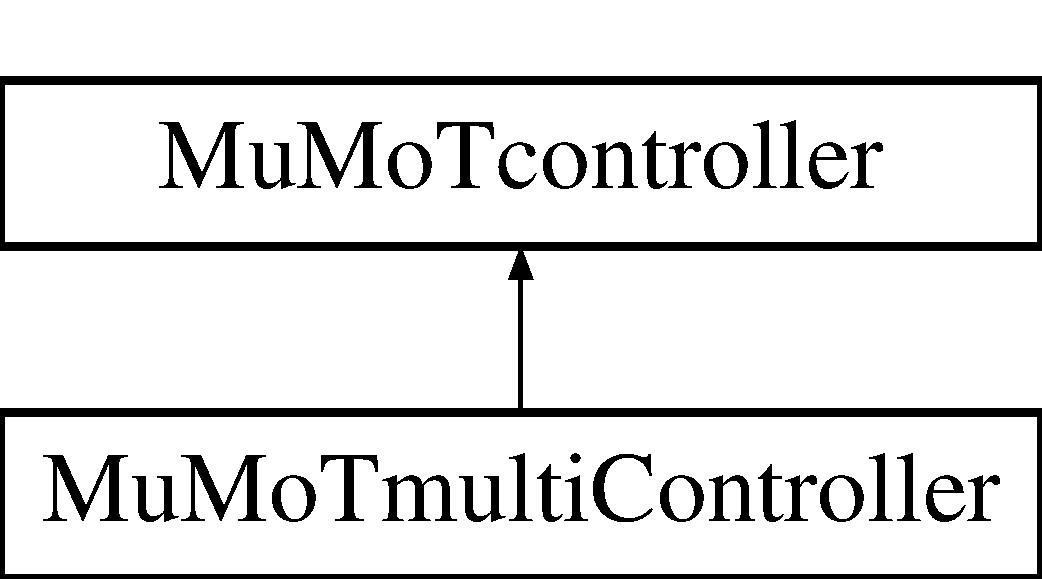
\includegraphics[height=2.000000cm]{class_mu_mo_t_1_1_mu_mo_t_1_1_mu_mo_tmulti_controller}
\end{center}
\end{figure}
\subsection*{Public Member Functions}
\begin{DoxyCompactItemize}
\item 
def \hyperlink{class_mu_mo_t_1_1_mu_mo_t_1_1_mu_mo_tmulti_controller_a5d04c30f0b85d1b7f2aa0fb1b23dca97}{\+\_\+\+\_\+init\+\_\+\+\_\+} (self, controllers, kwargs)
\end{DoxyCompactItemize}
\subsection*{Private Attributes}
\begin{DoxyCompactItemize}
\item 
\hyperlink{class_mu_mo_t_1_1_mu_mo_t_1_1_mu_mo_tmulti_controller_a909146a3c119c927727c7d533042b184}{\+\_\+silent}
\item 
\hyperlink{class_mu_mo_t_1_1_mu_mo_t_1_1_mu_mo_tmulti_controller_a018864aa22d2adb0d3958fb0adbce8e2}{\+\_\+progress\+Bar}
\begin{DoxyCompactList}\small\item\em presume this controller is a multi controller ( \end{DoxyCompactList}\item 
\hyperlink{class_mu_mo_t_1_1_mu_mo_t_1_1_mu_mo_tmulti_controller_a27dd8543b5188cdfe40f622d267fe2c5}{\+\_\+view}
\end{DoxyCompactItemize}
\subsection*{Static Private Attributes}
\begin{DoxyCompactItemize}
\item 
\hyperlink{class_mu_mo_t_1_1_mu_mo_t_1_1_mu_mo_tmulti_controller_a223edb833bfba55f245278156e2cb598}{\+\_\+replot\+Functions} = None
\begin{DoxyCompactList}\small\item\em replot function list to invoke on views \end{DoxyCompactList}\end{DoxyCompactItemize}


\subsection{Detailed Description}
multi-\/view controller 

\subsection{Constructor \& Destructor Documentation}
\mbox{\Hypertarget{class_mu_mo_t_1_1_mu_mo_t_1_1_mu_mo_tmulti_controller_a5d04c30f0b85d1b7f2aa0fb1b23dca97}\label{class_mu_mo_t_1_1_mu_mo_t_1_1_mu_mo_tmulti_controller_a5d04c30f0b85d1b7f2aa0fb1b23dca97}} 
\index{Mu\+Mo\+T\+::\+Mu\+Mo\+T\+::\+Mu\+Mo\+Tmulti\+Controller@{Mu\+Mo\+T\+::\+Mu\+Mo\+T\+::\+Mu\+Mo\+Tmulti\+Controller}!\+\_\+\+\_\+init\+\_\+\+\_\+@{\+\_\+\+\_\+init\+\_\+\+\_\+}}
\index{\+\_\+\+\_\+init\+\_\+\+\_\+@{\+\_\+\+\_\+init\+\_\+\+\_\+}!Mu\+Mo\+T\+::\+Mu\+Mo\+T\+::\+Mu\+Mo\+Tmulti\+Controller@{Mu\+Mo\+T\+::\+Mu\+Mo\+T\+::\+Mu\+Mo\+Tmulti\+Controller}}
\subsubsection{\texorpdfstring{\+\_\+\+\_\+init\+\_\+\+\_\+()}{\_\_init\_\_()}}
{\footnotesize\ttfamily def \+\_\+\+\_\+init\+\_\+\+\_\+ (\begin{DoxyParamCaption}\item[{}]{self,  }\item[{}]{controllers,  }\item[{}]{kwargs }\end{DoxyParamCaption})}



\subsection{Field Documentation}
\mbox{\Hypertarget{class_mu_mo_t_1_1_mu_mo_t_1_1_mu_mo_tmulti_controller_a018864aa22d2adb0d3958fb0adbce8e2}\label{class_mu_mo_t_1_1_mu_mo_t_1_1_mu_mo_tmulti_controller_a018864aa22d2adb0d3958fb0adbce8e2}} 
\index{Mu\+Mo\+T\+::\+Mu\+Mo\+T\+::\+Mu\+Mo\+Tmulti\+Controller@{Mu\+Mo\+T\+::\+Mu\+Mo\+T\+::\+Mu\+Mo\+Tmulti\+Controller}!\+\_\+progress\+Bar@{\+\_\+progress\+Bar}}
\index{\+\_\+progress\+Bar@{\+\_\+progress\+Bar}!Mu\+Mo\+T\+::\+Mu\+Mo\+T\+::\+Mu\+Mo\+Tmulti\+Controller@{Mu\+Mo\+T\+::\+Mu\+Mo\+T\+::\+Mu\+Mo\+Tmulti\+Controller}}
\subsubsection{\texorpdfstring{\+\_\+progress\+Bar}{\_progressBar}}
{\footnotesize\ttfamily \+\_\+progress\+Bar\hspace{0.3cm}{\ttfamily [private]}}



presume this controller is a multi controller ( 

\begin{DoxyRefDesc}{Todo}
\item[\hyperlink{todo__todo000034}{Todo}]check?) \end{DoxyRefDesc}
\mbox{\Hypertarget{class_mu_mo_t_1_1_mu_mo_t_1_1_mu_mo_tmulti_controller_a223edb833bfba55f245278156e2cb598}\label{class_mu_mo_t_1_1_mu_mo_t_1_1_mu_mo_tmulti_controller_a223edb833bfba55f245278156e2cb598}} 
\index{Mu\+Mo\+T\+::\+Mu\+Mo\+T\+::\+Mu\+Mo\+Tmulti\+Controller@{Mu\+Mo\+T\+::\+Mu\+Mo\+T\+::\+Mu\+Mo\+Tmulti\+Controller}!\+\_\+replot\+Functions@{\+\_\+replot\+Functions}}
\index{\+\_\+replot\+Functions@{\+\_\+replot\+Functions}!Mu\+Mo\+T\+::\+Mu\+Mo\+T\+::\+Mu\+Mo\+Tmulti\+Controller@{Mu\+Mo\+T\+::\+Mu\+Mo\+T\+::\+Mu\+Mo\+Tmulti\+Controller}}
\subsubsection{\texorpdfstring{\+\_\+replot\+Functions}{\_replotFunctions}}
{\footnotesize\ttfamily \+\_\+replot\+Functions = None\hspace{0.3cm}{\ttfamily [static]}, {\ttfamily [private]}}



replot function list to invoke on views 

\mbox{\Hypertarget{class_mu_mo_t_1_1_mu_mo_t_1_1_mu_mo_tmulti_controller_a909146a3c119c927727c7d533042b184}\label{class_mu_mo_t_1_1_mu_mo_t_1_1_mu_mo_tmulti_controller_a909146a3c119c927727c7d533042b184}} 
\index{Mu\+Mo\+T\+::\+Mu\+Mo\+T\+::\+Mu\+Mo\+Tmulti\+Controller@{Mu\+Mo\+T\+::\+Mu\+Mo\+T\+::\+Mu\+Mo\+Tmulti\+Controller}!\+\_\+silent@{\+\_\+silent}}
\index{\+\_\+silent@{\+\_\+silent}!Mu\+Mo\+T\+::\+Mu\+Mo\+T\+::\+Mu\+Mo\+Tmulti\+Controller@{Mu\+Mo\+T\+::\+Mu\+Mo\+T\+::\+Mu\+Mo\+Tmulti\+Controller}}
\subsubsection{\texorpdfstring{\+\_\+silent}{\_silent}}
{\footnotesize\ttfamily \+\_\+silent\hspace{0.3cm}{\ttfamily [private]}}

\mbox{\Hypertarget{class_mu_mo_t_1_1_mu_mo_t_1_1_mu_mo_tmulti_controller_a27dd8543b5188cdfe40f622d267fe2c5}\label{class_mu_mo_t_1_1_mu_mo_t_1_1_mu_mo_tmulti_controller_a27dd8543b5188cdfe40f622d267fe2c5}} 
\index{Mu\+Mo\+T\+::\+Mu\+Mo\+T\+::\+Mu\+Mo\+Tmulti\+Controller@{Mu\+Mo\+T\+::\+Mu\+Mo\+T\+::\+Mu\+Mo\+Tmulti\+Controller}!\+\_\+view@{\+\_\+view}}
\index{\+\_\+view@{\+\_\+view}!Mu\+Mo\+T\+::\+Mu\+Mo\+T\+::\+Mu\+Mo\+Tmulti\+Controller@{Mu\+Mo\+T\+::\+Mu\+Mo\+T\+::\+Mu\+Mo\+Tmulti\+Controller}}
\subsubsection{\texorpdfstring{\+\_\+view}{\_view}}
{\footnotesize\ttfamily \+\_\+view\hspace{0.3cm}{\ttfamily [private]}}



The documentation for this class was generated from the following file\+:\begin{DoxyCompactItemize}
\item 
Mu\+Mo\+T/\hyperlink{_mu_mo_t_8py}{Mu\+Mo\+T.\+py}\end{DoxyCompactItemize}

\hypertarget{class_mu_mo_t_1_1_mu_mo_t_1_1_mu_mo_tmulti_view}{}\section{Mu\+Mo\+Tmulti\+View Class Reference}
\label{class_mu_mo_t_1_1_mu_mo_t_1_1_mu_mo_tmulti_view}\index{Mu\+Mo\+Tmulti\+View@{Mu\+Mo\+Tmulti\+View}}


multi-\/view view (tied closely to \hyperlink{class_mu_mo_t_1_1_mu_mo_t_1_1_mu_mo_tmulti_controller}{Mu\+Mo\+Tmulti\+Controller})  


Inheritance diagram for Mu\+Mo\+Tmulti\+View\+:\begin{figure}[H]
\begin{center}
\leavevmode
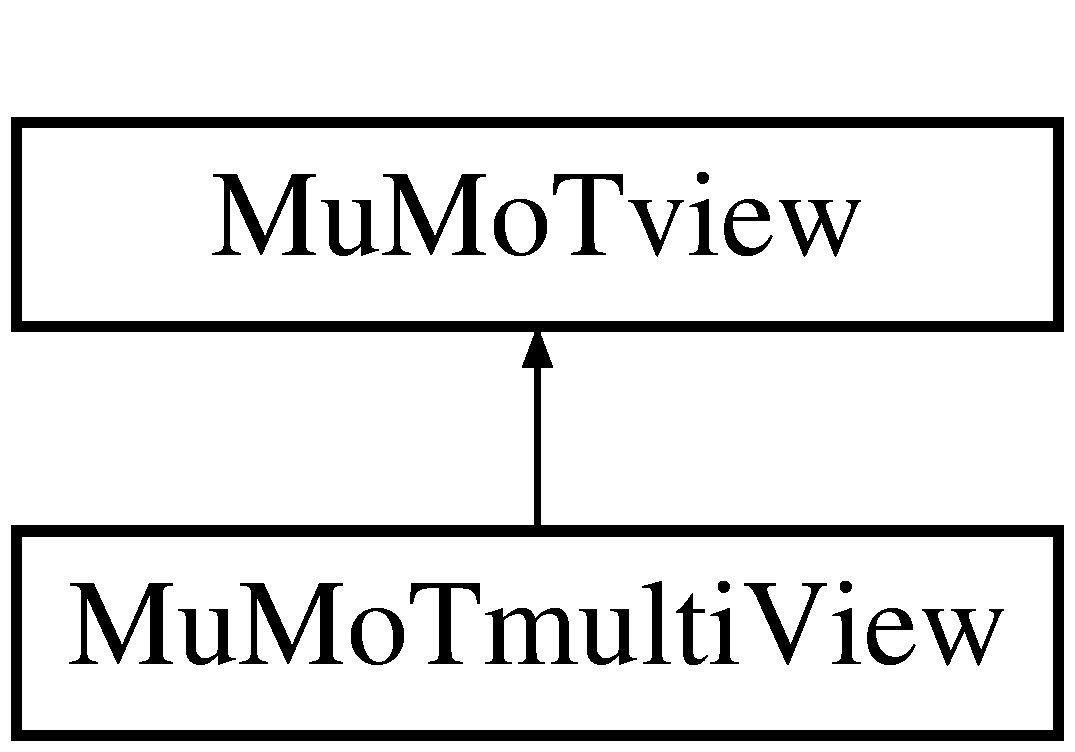
\includegraphics[height=2.000000cm]{class_mu_mo_t_1_1_mu_mo_t_1_1_mu_mo_tmulti_view}
\end{center}
\end{figure}
\subsection*{Public Member Functions}
\begin{DoxyCompactItemize}
\item 
def \hyperlink{class_mu_mo_t_1_1_mu_mo_t_1_1_mu_mo_tmulti_view_aa355c85c06db29c1df7b6505493d5354}{\+\_\+\+\_\+init\+\_\+\+\_\+} (self, controller, views, sub\+Plot\+Num, kwargs)
\end{DoxyCompactItemize}
\subsection*{Private Member Functions}
\begin{DoxyCompactItemize}
\item 
def \hyperlink{class_mu_mo_t_1_1_mu_mo_t_1_1_mu_mo_tmulti_view_aaff21bb2a6ebdaed50f2f2fb67d0bf5c}{\+\_\+plot} (self)
\item 
def \hyperlink{class_mu_mo_t_1_1_mu_mo_t_1_1_mu_mo_tmulti_view_abfc1e19ed53c088799d1f499bc010f7f}{\+\_\+set\+Log} (self, log)
\item 
def \hyperlink{class_mu_mo_t_1_1_mu_mo_t_1_1_mu_mo_tmulti_view_a3af54c33f997937b14f422e772d5280a}{\+\_\+print\+\_\+standalone\+\_\+view\+\_\+cmd} (self)
\end{DoxyCompactItemize}
\subsection*{Private Attributes}
\begin{DoxyCompactItemize}
\item 
\hyperlink{class_mu_mo_t_1_1_mu_mo_t_1_1_mu_mo_tmulti_view_ace48ed03490093d8f44cde91e2f1e86e}{\+\_\+generating\+Command}
\end{DoxyCompactItemize}
\subsection*{Static Private Attributes}
\begin{DoxyCompactItemize}
\item 
\hyperlink{class_mu_mo_t_1_1_mu_mo_t_1_1_mu_mo_tmulti_view_af533f289cf818694f54ab8bd57083537}{\+\_\+views} = None
\begin{DoxyCompactList}\small\item\em view list \end{DoxyCompactList}\item 
\hyperlink{class_mu_mo_t_1_1_mu_mo_t_1_1_mu_mo_tmulti_view_a302b03ed97754a48ed830efba51e8d37}{\+\_\+axes} = None
\begin{DoxyCompactList}\small\item\em axes are used for subplots (\textquotesingle{}share\+Axes = True\textquotesingle{}) \end{DoxyCompactList}\item 
\hyperlink{class_mu_mo_t_1_1_mu_mo_t_1_1_mu_mo_tmulti_view_a9b9e6dc4ee0823b917bb0ee0d636f84d}{\+\_\+sub\+Plot\+Num} = None
\begin{DoxyCompactList}\small\item\em number of subplots \end{DoxyCompactList}\item 
\hyperlink{class_mu_mo_t_1_1_mu_mo_t_1_1_mu_mo_tmulti_view_a7943427bc009bd206f958f785e744381}{\+\_\+num\+Rows} = None
\begin{DoxyCompactList}\small\item\em subplot rows \end{DoxyCompactList}\item 
\hyperlink{class_mu_mo_t_1_1_mu_mo_t_1_1_mu_mo_tmulti_view_ac14e35edb2af762045879408234589d5}{\+\_\+num\+Columns} = None
\begin{DoxyCompactList}\small\item\em subplot columns \end{DoxyCompactList}\item 
\hyperlink{class_mu_mo_t_1_1_mu_mo_t_1_1_mu_mo_tmulti_view_a564f1d8714ede71e8f36f29d64193518}{\+\_\+share\+Axes} = None
\begin{DoxyCompactList}\small\item\em use common axes for all plots (False = use subplots) \end{DoxyCompactList}\end{DoxyCompactItemize}
\subsection*{Additional Inherited Members}


\subsection{Detailed Description}
multi-\/view view (tied closely to \hyperlink{class_mu_mo_t_1_1_mu_mo_t_1_1_mu_mo_tmulti_controller}{Mu\+Mo\+Tmulti\+Controller}) 

\subsection{Constructor \& Destructor Documentation}
\mbox{\Hypertarget{class_mu_mo_t_1_1_mu_mo_t_1_1_mu_mo_tmulti_view_aa355c85c06db29c1df7b6505493d5354}\label{class_mu_mo_t_1_1_mu_mo_t_1_1_mu_mo_tmulti_view_aa355c85c06db29c1df7b6505493d5354}} 
\index{Mu\+Mo\+T\+::\+Mu\+Mo\+T\+::\+Mu\+Mo\+Tmulti\+View@{Mu\+Mo\+T\+::\+Mu\+Mo\+T\+::\+Mu\+Mo\+Tmulti\+View}!\+\_\+\+\_\+init\+\_\+\+\_\+@{\+\_\+\+\_\+init\+\_\+\+\_\+}}
\index{\+\_\+\+\_\+init\+\_\+\+\_\+@{\+\_\+\+\_\+init\+\_\+\+\_\+}!Mu\+Mo\+T\+::\+Mu\+Mo\+T\+::\+Mu\+Mo\+Tmulti\+View@{Mu\+Mo\+T\+::\+Mu\+Mo\+T\+::\+Mu\+Mo\+Tmulti\+View}}
\subsubsection{\texorpdfstring{\+\_\+\+\_\+init\+\_\+\+\_\+()}{\_\_init\_\_()}}
{\footnotesize\ttfamily def \+\_\+\+\_\+init\+\_\+\+\_\+ (\begin{DoxyParamCaption}\item[{}]{self,  }\item[{}]{controller,  }\item[{}]{views,  }\item[{}]{sub\+Plot\+Num,  }\item[{}]{kwargs }\end{DoxyParamCaption})}



\subsection{Member Function Documentation}
\mbox{\Hypertarget{class_mu_mo_t_1_1_mu_mo_t_1_1_mu_mo_tmulti_view_aaff21bb2a6ebdaed50f2f2fb67d0bf5c}\label{class_mu_mo_t_1_1_mu_mo_t_1_1_mu_mo_tmulti_view_aaff21bb2a6ebdaed50f2f2fb67d0bf5c}} 
\index{Mu\+Mo\+T\+::\+Mu\+Mo\+T\+::\+Mu\+Mo\+Tmulti\+View@{Mu\+Mo\+T\+::\+Mu\+Mo\+T\+::\+Mu\+Mo\+Tmulti\+View}!\+\_\+plot@{\+\_\+plot}}
\index{\+\_\+plot@{\+\_\+plot}!Mu\+Mo\+T\+::\+Mu\+Mo\+T\+::\+Mu\+Mo\+Tmulti\+View@{Mu\+Mo\+T\+::\+Mu\+Mo\+T\+::\+Mu\+Mo\+Tmulti\+View}}
\subsubsection{\texorpdfstring{\+\_\+plot()}{\_plot()}}
{\footnotesize\ttfamily def \+\_\+plot (\begin{DoxyParamCaption}\item[{}]{self }\end{DoxyParamCaption})\hspace{0.3cm}{\ttfamily [private]}}

\mbox{\Hypertarget{class_mu_mo_t_1_1_mu_mo_t_1_1_mu_mo_tmulti_view_a3af54c33f997937b14f422e772d5280a}\label{class_mu_mo_t_1_1_mu_mo_t_1_1_mu_mo_tmulti_view_a3af54c33f997937b14f422e772d5280a}} 
\index{Mu\+Mo\+T\+::\+Mu\+Mo\+T\+::\+Mu\+Mo\+Tmulti\+View@{Mu\+Mo\+T\+::\+Mu\+Mo\+T\+::\+Mu\+Mo\+Tmulti\+View}!\+\_\+print\+\_\+standalone\+\_\+view\+\_\+cmd@{\+\_\+print\+\_\+standalone\+\_\+view\+\_\+cmd}}
\index{\+\_\+print\+\_\+standalone\+\_\+view\+\_\+cmd@{\+\_\+print\+\_\+standalone\+\_\+view\+\_\+cmd}!Mu\+Mo\+T\+::\+Mu\+Mo\+T\+::\+Mu\+Mo\+Tmulti\+View@{Mu\+Mo\+T\+::\+Mu\+Mo\+T\+::\+Mu\+Mo\+Tmulti\+View}}
\subsubsection{\texorpdfstring{\+\_\+print\+\_\+standalone\+\_\+view\+\_\+cmd()}{\_print\_standalone\_view\_cmd()}}
{\footnotesize\ttfamily def \+\_\+print\+\_\+standalone\+\_\+view\+\_\+cmd (\begin{DoxyParamCaption}\item[{}]{self }\end{DoxyParamCaption})\hspace{0.3cm}{\ttfamily [private]}}

\mbox{\Hypertarget{class_mu_mo_t_1_1_mu_mo_t_1_1_mu_mo_tmulti_view_abfc1e19ed53c088799d1f499bc010f7f}\label{class_mu_mo_t_1_1_mu_mo_t_1_1_mu_mo_tmulti_view_abfc1e19ed53c088799d1f499bc010f7f}} 
\index{Mu\+Mo\+T\+::\+Mu\+Mo\+T\+::\+Mu\+Mo\+Tmulti\+View@{Mu\+Mo\+T\+::\+Mu\+Mo\+T\+::\+Mu\+Mo\+Tmulti\+View}!\+\_\+set\+Log@{\+\_\+set\+Log}}
\index{\+\_\+set\+Log@{\+\_\+set\+Log}!Mu\+Mo\+T\+::\+Mu\+Mo\+T\+::\+Mu\+Mo\+Tmulti\+View@{Mu\+Mo\+T\+::\+Mu\+Mo\+T\+::\+Mu\+Mo\+Tmulti\+View}}
\subsubsection{\texorpdfstring{\+\_\+set\+Log()}{\_setLog()}}
{\footnotesize\ttfamily def \+\_\+set\+Log (\begin{DoxyParamCaption}\item[{}]{self,  }\item[{}]{log }\end{DoxyParamCaption})\hspace{0.3cm}{\ttfamily [private]}}



\subsection{Field Documentation}
\mbox{\Hypertarget{class_mu_mo_t_1_1_mu_mo_t_1_1_mu_mo_tmulti_view_a302b03ed97754a48ed830efba51e8d37}\label{class_mu_mo_t_1_1_mu_mo_t_1_1_mu_mo_tmulti_view_a302b03ed97754a48ed830efba51e8d37}} 
\index{Mu\+Mo\+T\+::\+Mu\+Mo\+T\+::\+Mu\+Mo\+Tmulti\+View@{Mu\+Mo\+T\+::\+Mu\+Mo\+T\+::\+Mu\+Mo\+Tmulti\+View}!\+\_\+axes@{\+\_\+axes}}
\index{\+\_\+axes@{\+\_\+axes}!Mu\+Mo\+T\+::\+Mu\+Mo\+T\+::\+Mu\+Mo\+Tmulti\+View@{Mu\+Mo\+T\+::\+Mu\+Mo\+T\+::\+Mu\+Mo\+Tmulti\+View}}
\subsubsection{\texorpdfstring{\+\_\+axes}{\_axes}}
{\footnotesize\ttfamily \+\_\+axes = None\hspace{0.3cm}{\ttfamily [static]}, {\ttfamily [private]}}



axes are used for subplots (\textquotesingle{}share\+Axes = True\textquotesingle{}) 

\mbox{\Hypertarget{class_mu_mo_t_1_1_mu_mo_t_1_1_mu_mo_tmulti_view_ace48ed03490093d8f44cde91e2f1e86e}\label{class_mu_mo_t_1_1_mu_mo_t_1_1_mu_mo_tmulti_view_ace48ed03490093d8f44cde91e2f1e86e}} 
\index{Mu\+Mo\+T\+::\+Mu\+Mo\+T\+::\+Mu\+Mo\+Tmulti\+View@{Mu\+Mo\+T\+::\+Mu\+Mo\+T\+::\+Mu\+Mo\+Tmulti\+View}!\+\_\+generating\+Command@{\+\_\+generating\+Command}}
\index{\+\_\+generating\+Command@{\+\_\+generating\+Command}!Mu\+Mo\+T\+::\+Mu\+Mo\+T\+::\+Mu\+Mo\+Tmulti\+View@{Mu\+Mo\+T\+::\+Mu\+Mo\+T\+::\+Mu\+Mo\+Tmulti\+View}}
\subsubsection{\texorpdfstring{\+\_\+generating\+Command}{\_generatingCommand}}
{\footnotesize\ttfamily \+\_\+generating\+Command\hspace{0.3cm}{\ttfamily [private]}}

\mbox{\Hypertarget{class_mu_mo_t_1_1_mu_mo_t_1_1_mu_mo_tmulti_view_ac14e35edb2af762045879408234589d5}\label{class_mu_mo_t_1_1_mu_mo_t_1_1_mu_mo_tmulti_view_ac14e35edb2af762045879408234589d5}} 
\index{Mu\+Mo\+T\+::\+Mu\+Mo\+T\+::\+Mu\+Mo\+Tmulti\+View@{Mu\+Mo\+T\+::\+Mu\+Mo\+T\+::\+Mu\+Mo\+Tmulti\+View}!\+\_\+num\+Columns@{\+\_\+num\+Columns}}
\index{\+\_\+num\+Columns@{\+\_\+num\+Columns}!Mu\+Mo\+T\+::\+Mu\+Mo\+T\+::\+Mu\+Mo\+Tmulti\+View@{Mu\+Mo\+T\+::\+Mu\+Mo\+T\+::\+Mu\+Mo\+Tmulti\+View}}
\subsubsection{\texorpdfstring{\+\_\+num\+Columns}{\_numColumns}}
{\footnotesize\ttfamily \+\_\+num\+Columns = None\hspace{0.3cm}{\ttfamily [static]}, {\ttfamily [private]}}



subplot columns 

\mbox{\Hypertarget{class_mu_mo_t_1_1_mu_mo_t_1_1_mu_mo_tmulti_view_a7943427bc009bd206f958f785e744381}\label{class_mu_mo_t_1_1_mu_mo_t_1_1_mu_mo_tmulti_view_a7943427bc009bd206f958f785e744381}} 
\index{Mu\+Mo\+T\+::\+Mu\+Mo\+T\+::\+Mu\+Mo\+Tmulti\+View@{Mu\+Mo\+T\+::\+Mu\+Mo\+T\+::\+Mu\+Mo\+Tmulti\+View}!\+\_\+num\+Rows@{\+\_\+num\+Rows}}
\index{\+\_\+num\+Rows@{\+\_\+num\+Rows}!Mu\+Mo\+T\+::\+Mu\+Mo\+T\+::\+Mu\+Mo\+Tmulti\+View@{Mu\+Mo\+T\+::\+Mu\+Mo\+T\+::\+Mu\+Mo\+Tmulti\+View}}
\subsubsection{\texorpdfstring{\+\_\+num\+Rows}{\_numRows}}
{\footnotesize\ttfamily \+\_\+num\+Rows = None\hspace{0.3cm}{\ttfamily [static]}, {\ttfamily [private]}}



subplot rows 

\mbox{\Hypertarget{class_mu_mo_t_1_1_mu_mo_t_1_1_mu_mo_tmulti_view_a564f1d8714ede71e8f36f29d64193518}\label{class_mu_mo_t_1_1_mu_mo_t_1_1_mu_mo_tmulti_view_a564f1d8714ede71e8f36f29d64193518}} 
\index{Mu\+Mo\+T\+::\+Mu\+Mo\+T\+::\+Mu\+Mo\+Tmulti\+View@{Mu\+Mo\+T\+::\+Mu\+Mo\+T\+::\+Mu\+Mo\+Tmulti\+View}!\+\_\+share\+Axes@{\+\_\+share\+Axes}}
\index{\+\_\+share\+Axes@{\+\_\+share\+Axes}!Mu\+Mo\+T\+::\+Mu\+Mo\+T\+::\+Mu\+Mo\+Tmulti\+View@{Mu\+Mo\+T\+::\+Mu\+Mo\+T\+::\+Mu\+Mo\+Tmulti\+View}}
\subsubsection{\texorpdfstring{\+\_\+share\+Axes}{\_shareAxes}}
{\footnotesize\ttfamily \+\_\+share\+Axes = None\hspace{0.3cm}{\ttfamily [static]}, {\ttfamily [private]}}



use common axes for all plots (False = use subplots) 

\mbox{\Hypertarget{class_mu_mo_t_1_1_mu_mo_t_1_1_mu_mo_tmulti_view_a9b9e6dc4ee0823b917bb0ee0d636f84d}\label{class_mu_mo_t_1_1_mu_mo_t_1_1_mu_mo_tmulti_view_a9b9e6dc4ee0823b917bb0ee0d636f84d}} 
\index{Mu\+Mo\+T\+::\+Mu\+Mo\+T\+::\+Mu\+Mo\+Tmulti\+View@{Mu\+Mo\+T\+::\+Mu\+Mo\+T\+::\+Mu\+Mo\+Tmulti\+View}!\+\_\+sub\+Plot\+Num@{\+\_\+sub\+Plot\+Num}}
\index{\+\_\+sub\+Plot\+Num@{\+\_\+sub\+Plot\+Num}!Mu\+Mo\+T\+::\+Mu\+Mo\+T\+::\+Mu\+Mo\+Tmulti\+View@{Mu\+Mo\+T\+::\+Mu\+Mo\+T\+::\+Mu\+Mo\+Tmulti\+View}}
\subsubsection{\texorpdfstring{\+\_\+sub\+Plot\+Num}{\_subPlotNum}}
{\footnotesize\ttfamily \+\_\+sub\+Plot\+Num = None\hspace{0.3cm}{\ttfamily [static]}, {\ttfamily [private]}}



number of subplots 

\mbox{\Hypertarget{class_mu_mo_t_1_1_mu_mo_t_1_1_mu_mo_tmulti_view_af533f289cf818694f54ab8bd57083537}\label{class_mu_mo_t_1_1_mu_mo_t_1_1_mu_mo_tmulti_view_af533f289cf818694f54ab8bd57083537}} 
\index{Mu\+Mo\+T\+::\+Mu\+Mo\+T\+::\+Mu\+Mo\+Tmulti\+View@{Mu\+Mo\+T\+::\+Mu\+Mo\+T\+::\+Mu\+Mo\+Tmulti\+View}!\+\_\+views@{\+\_\+views}}
\index{\+\_\+views@{\+\_\+views}!Mu\+Mo\+T\+::\+Mu\+Mo\+T\+::\+Mu\+Mo\+Tmulti\+View@{Mu\+Mo\+T\+::\+Mu\+Mo\+T\+::\+Mu\+Mo\+Tmulti\+View}}
\subsubsection{\texorpdfstring{\+\_\+views}{\_views}}
{\footnotesize\ttfamily \+\_\+views = None\hspace{0.3cm}{\ttfamily [static]}, {\ttfamily [private]}}



view list 



The documentation for this class was generated from the following file\+:\begin{DoxyCompactItemize}
\item 
Mu\+Mo\+T/\hyperlink{_mu_mo_t_8py}{Mu\+Mo\+T.\+py}\end{DoxyCompactItemize}

\hypertarget{class_mu_mo_t_1_1_mu_mo_t_1_1_mu_mo_tnoise_view}{}\section{Mu\+Mo\+Tnoise\+View Class Reference}
\label{class_mu_mo_t_1_1_mu_mo_t_1_1_mu_mo_tnoise_view}\index{Mu\+Mo\+Tnoise\+View@{Mu\+Mo\+Tnoise\+View}}


stream plot with noise ellipses view on model  


Inheritance diagram for Mu\+Mo\+Tnoise\+View\+:\begin{figure}[H]
\begin{center}
\leavevmode
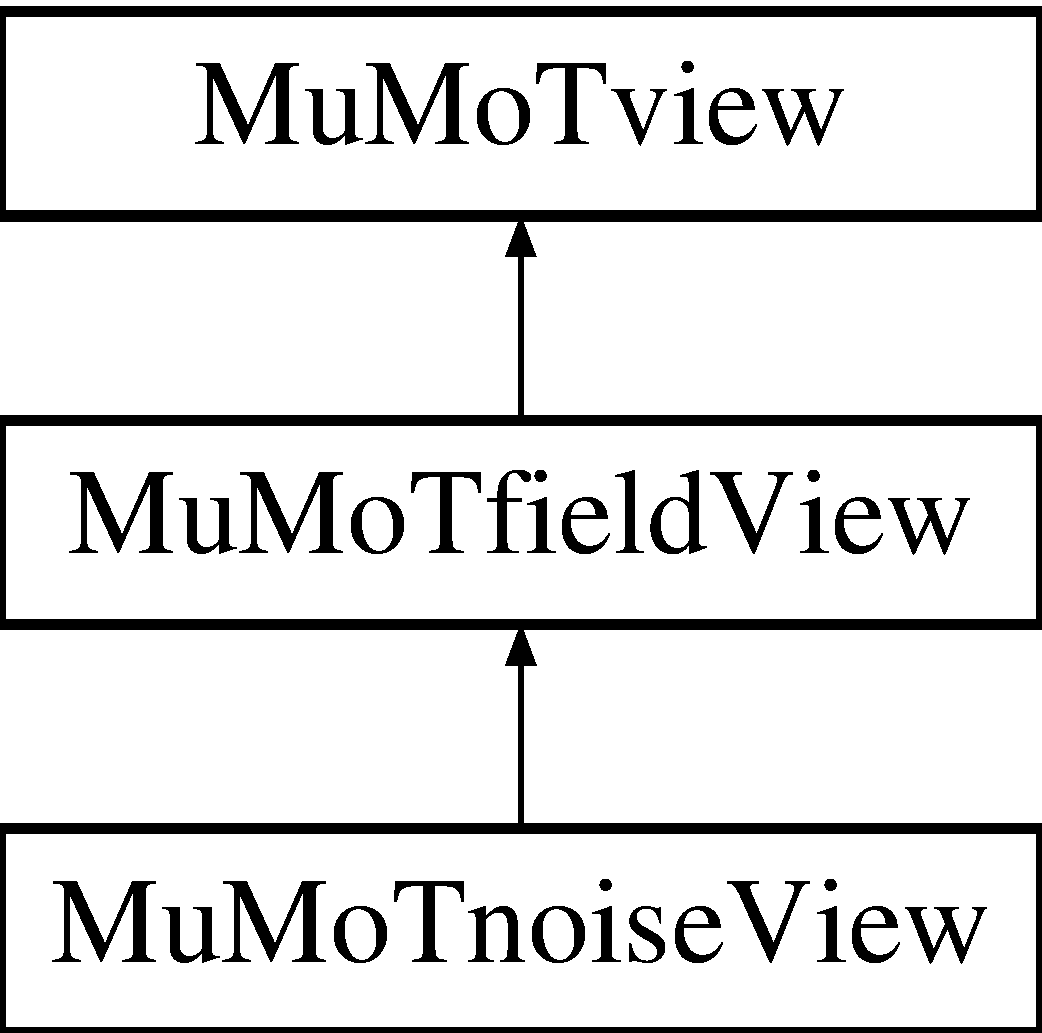
\includegraphics[height=3.000000cm]{class_mu_mo_t_1_1_mu_mo_t_1_1_mu_mo_tnoise_view}
\end{center}
\end{figure}
\subsection*{Public Member Functions}
\begin{DoxyCompactItemize}
\item 
def \hyperlink{class_mu_mo_t_1_1_mu_mo_t_1_1_mu_mo_tnoise_view_a84e681320c67584b27e757b9bf8e80af}{\+\_\+\+\_\+init\+\_\+\+\_\+} (self, model, controller, S\+O\+L\+\_\+2nd\+Ord, state\+Variable1, state\+Variable2, state\+Variable3=None, figure=None, params=None, kwargs)
\end{DoxyCompactItemize}
\subsection*{Private Member Functions}
\begin{DoxyCompactItemize}
\item 
def \hyperlink{class_mu_mo_t_1_1_mu_mo_t_1_1_mu_mo_tnoise_view_a50d59419298116f738a98c864afb9d89}{\+\_\+plot\+\_\+field} (self)
\end{DoxyCompactItemize}
\subsection*{Private Attributes}
\begin{DoxyCompactItemize}
\item 
\hyperlink{class_mu_mo_t_1_1_mu_mo_t_1_1_mu_mo_tnoise_view_ace48ed03490093d8f44cde91e2f1e86e}{\+\_\+generating\+Command}
\item 
\hyperlink{class_mu_mo_t_1_1_mu_mo_t_1_1_mu_mo_tnoise_view_ac83a924ad62a2461d65b5c9bf9d27453}{\+\_\+show\+Fixed\+Points}
\end{DoxyCompactItemize}
\subsection*{Static Private Attributes}
\begin{DoxyCompactItemize}
\item 
\hyperlink{class_mu_mo_t_1_1_mu_mo_t_1_1_mu_mo_tnoise_view_a296250af1fa7174eea4104b344417b90}{\+\_\+\+S\+O\+L\+\_\+1st\+Order\+Mom\+Dict} = None
\begin{DoxyCompactList}\small\item\em solution 1st order moments (noise in v\+KE) \end{DoxyCompactList}\item 
\hyperlink{class_mu_mo_t_1_1_mu_mo_t_1_1_mu_mo_tnoise_view_ad481992f34b8ccf5d64d223cc55631f1}{\+\_\+\+Noise\+Subs1st\+Order} = None
\begin{DoxyCompactList}\small\item\em replacement dictionary for symbols of 1st order moments \end{DoxyCompactList}\item 
\hyperlink{class_mu_mo_t_1_1_mu_mo_t_1_1_mu_mo_tnoise_view_a791676592e6ef1620caf2efb21c9d398}{\+\_\+\+S\+O\+L\+\_\+2nd\+Ord\+Mom\+Dict} = None
\begin{DoxyCompactList}\small\item\em solution 2nd order moments (noise in v\+KE) \end{DoxyCompactList}\item 
\hyperlink{class_mu_mo_t_1_1_mu_mo_t_1_1_mu_mo_tnoise_view_a3a833e83790a135218b980c75d031bc2}{\+\_\+\+Noise\+Subs2nd\+Order} = None
\begin{DoxyCompactList}\small\item\em replacement dictionary for symbols of 2nd order moments \end{DoxyCompactList}\item 
\hyperlink{class_mu_mo_t_1_1_mu_mo_t_1_1_mu_mo_tnoise_view_a67947eab5f25a49aed08d7ba84992bdb}{\+\_\+check\+Reactants} = None
\begin{DoxyCompactList}\small\item\em set for checking number of time-\/dependent reactants \end{DoxyCompactList}\item 
\hyperlink{class_mu_mo_t_1_1_mu_mo_t_1_1_mu_mo_tnoise_view_ac697abee533ce7967dba1ca8450f6153}{\+\_\+check\+Const\+Reactants} = None
\begin{DoxyCompactList}\small\item\em set for checking constant reactants \end{DoxyCompactList}\item 
\hyperlink{class_mu_mo_t_1_1_mu_mo_t_1_1_mu_mo_tnoise_view_abeed4a9b1de71e913d16fc6363f13f03}{\+\_\+noise\+Stat\+Sol} = None
\end{DoxyCompactItemize}
\subsection*{Additional Inherited Members}


\subsection{Detailed Description}
stream plot with noise ellipses view on model 

\subsection{Constructor \& Destructor Documentation}
\mbox{\Hypertarget{class_mu_mo_t_1_1_mu_mo_t_1_1_mu_mo_tnoise_view_a84e681320c67584b27e757b9bf8e80af}\label{class_mu_mo_t_1_1_mu_mo_t_1_1_mu_mo_tnoise_view_a84e681320c67584b27e757b9bf8e80af}} 
\index{Mu\+Mo\+T\+::\+Mu\+Mo\+T\+::\+Mu\+Mo\+Tnoise\+View@{Mu\+Mo\+T\+::\+Mu\+Mo\+T\+::\+Mu\+Mo\+Tnoise\+View}!\+\_\+\+\_\+init\+\_\+\+\_\+@{\+\_\+\+\_\+init\+\_\+\+\_\+}}
\index{\+\_\+\+\_\+init\+\_\+\+\_\+@{\+\_\+\+\_\+init\+\_\+\+\_\+}!Mu\+Mo\+T\+::\+Mu\+Mo\+T\+::\+Mu\+Mo\+Tnoise\+View@{Mu\+Mo\+T\+::\+Mu\+Mo\+T\+::\+Mu\+Mo\+Tnoise\+View}}
\subsubsection{\texorpdfstring{\+\_\+\+\_\+init\+\_\+\+\_\+()}{\_\_init\_\_()}}
{\footnotesize\ttfamily def \+\_\+\+\_\+init\+\_\+\+\_\+ (\begin{DoxyParamCaption}\item[{}]{self,  }\item[{}]{model,  }\item[{}]{controller,  }\item[{}]{S\+O\+L\+\_\+2nd\+Ord,  }\item[{}]{state\+Variable1,  }\item[{}]{state\+Variable2,  }\item[{}]{state\+Variable3 = {\ttfamily None},  }\item[{}]{figure = {\ttfamily None},  }\item[{}]{params = {\ttfamily None},  }\item[{}]{kwargs }\end{DoxyParamCaption})}



\subsection{Member Function Documentation}
\mbox{\Hypertarget{class_mu_mo_t_1_1_mu_mo_t_1_1_mu_mo_tnoise_view_a50d59419298116f738a98c864afb9d89}\label{class_mu_mo_t_1_1_mu_mo_t_1_1_mu_mo_tnoise_view_a50d59419298116f738a98c864afb9d89}} 
\index{Mu\+Mo\+T\+::\+Mu\+Mo\+T\+::\+Mu\+Mo\+Tnoise\+View@{Mu\+Mo\+T\+::\+Mu\+Mo\+T\+::\+Mu\+Mo\+Tnoise\+View}!\+\_\+plot\+\_\+field@{\+\_\+plot\+\_\+field}}
\index{\+\_\+plot\+\_\+field@{\+\_\+plot\+\_\+field}!Mu\+Mo\+T\+::\+Mu\+Mo\+T\+::\+Mu\+Mo\+Tnoise\+View@{Mu\+Mo\+T\+::\+Mu\+Mo\+T\+::\+Mu\+Mo\+Tnoise\+View}}
\subsubsection{\texorpdfstring{\+\_\+plot\+\_\+field()}{\_plot\_field()}}
{\footnotesize\ttfamily def \+\_\+plot\+\_\+field (\begin{DoxyParamCaption}\item[{}]{self }\end{DoxyParamCaption})\hspace{0.3cm}{\ttfamily [private]}}



\subsection{Field Documentation}
\mbox{\Hypertarget{class_mu_mo_t_1_1_mu_mo_t_1_1_mu_mo_tnoise_view_ac697abee533ce7967dba1ca8450f6153}\label{class_mu_mo_t_1_1_mu_mo_t_1_1_mu_mo_tnoise_view_ac697abee533ce7967dba1ca8450f6153}} 
\index{Mu\+Mo\+T\+::\+Mu\+Mo\+T\+::\+Mu\+Mo\+Tnoise\+View@{Mu\+Mo\+T\+::\+Mu\+Mo\+T\+::\+Mu\+Mo\+Tnoise\+View}!\+\_\+check\+Const\+Reactants@{\+\_\+check\+Const\+Reactants}}
\index{\+\_\+check\+Const\+Reactants@{\+\_\+check\+Const\+Reactants}!Mu\+Mo\+T\+::\+Mu\+Mo\+T\+::\+Mu\+Mo\+Tnoise\+View@{Mu\+Mo\+T\+::\+Mu\+Mo\+T\+::\+Mu\+Mo\+Tnoise\+View}}
\subsubsection{\texorpdfstring{\+\_\+check\+Const\+Reactants}{\_checkConstReactants}}
{\footnotesize\ttfamily \+\_\+check\+Const\+Reactants = None\hspace{0.3cm}{\ttfamily [static]}, {\ttfamily [private]}}



set for checking constant reactants 

\mbox{\Hypertarget{class_mu_mo_t_1_1_mu_mo_t_1_1_mu_mo_tnoise_view_a67947eab5f25a49aed08d7ba84992bdb}\label{class_mu_mo_t_1_1_mu_mo_t_1_1_mu_mo_tnoise_view_a67947eab5f25a49aed08d7ba84992bdb}} 
\index{Mu\+Mo\+T\+::\+Mu\+Mo\+T\+::\+Mu\+Mo\+Tnoise\+View@{Mu\+Mo\+T\+::\+Mu\+Mo\+T\+::\+Mu\+Mo\+Tnoise\+View}!\+\_\+check\+Reactants@{\+\_\+check\+Reactants}}
\index{\+\_\+check\+Reactants@{\+\_\+check\+Reactants}!Mu\+Mo\+T\+::\+Mu\+Mo\+T\+::\+Mu\+Mo\+Tnoise\+View@{Mu\+Mo\+T\+::\+Mu\+Mo\+T\+::\+Mu\+Mo\+Tnoise\+View}}
\subsubsection{\texorpdfstring{\+\_\+check\+Reactants}{\_checkReactants}}
{\footnotesize\ttfamily \+\_\+check\+Reactants = None\hspace{0.3cm}{\ttfamily [static]}, {\ttfamily [private]}}



set for checking number of time-\/dependent reactants 

\mbox{\Hypertarget{class_mu_mo_t_1_1_mu_mo_t_1_1_mu_mo_tnoise_view_ace48ed03490093d8f44cde91e2f1e86e}\label{class_mu_mo_t_1_1_mu_mo_t_1_1_mu_mo_tnoise_view_ace48ed03490093d8f44cde91e2f1e86e}} 
\index{Mu\+Mo\+T\+::\+Mu\+Mo\+T\+::\+Mu\+Mo\+Tnoise\+View@{Mu\+Mo\+T\+::\+Mu\+Mo\+T\+::\+Mu\+Mo\+Tnoise\+View}!\+\_\+generating\+Command@{\+\_\+generating\+Command}}
\index{\+\_\+generating\+Command@{\+\_\+generating\+Command}!Mu\+Mo\+T\+::\+Mu\+Mo\+T\+::\+Mu\+Mo\+Tnoise\+View@{Mu\+Mo\+T\+::\+Mu\+Mo\+T\+::\+Mu\+Mo\+Tnoise\+View}}
\subsubsection{\texorpdfstring{\+\_\+generating\+Command}{\_generatingCommand}}
{\footnotesize\ttfamily \+\_\+generating\+Command\hspace{0.3cm}{\ttfamily [private]}}

\mbox{\Hypertarget{class_mu_mo_t_1_1_mu_mo_t_1_1_mu_mo_tnoise_view_abeed4a9b1de71e913d16fc6363f13f03}\label{class_mu_mo_t_1_1_mu_mo_t_1_1_mu_mo_tnoise_view_abeed4a9b1de71e913d16fc6363f13f03}} 
\index{Mu\+Mo\+T\+::\+Mu\+Mo\+T\+::\+Mu\+Mo\+Tnoise\+View@{Mu\+Mo\+T\+::\+Mu\+Mo\+T\+::\+Mu\+Mo\+Tnoise\+View}!\+\_\+noise\+Stat\+Sol@{\+\_\+noise\+Stat\+Sol}}
\index{\+\_\+noise\+Stat\+Sol@{\+\_\+noise\+Stat\+Sol}!Mu\+Mo\+T\+::\+Mu\+Mo\+T\+::\+Mu\+Mo\+Tnoise\+View@{Mu\+Mo\+T\+::\+Mu\+Mo\+T\+::\+Mu\+Mo\+Tnoise\+View}}
\subsubsection{\texorpdfstring{\+\_\+noise\+Stat\+Sol}{\_noiseStatSol}}
{\footnotesize\ttfamily \+\_\+noise\+Stat\+Sol = None\hspace{0.3cm}{\ttfamily [static]}, {\ttfamily [private]}}

\mbox{\Hypertarget{class_mu_mo_t_1_1_mu_mo_t_1_1_mu_mo_tnoise_view_ad481992f34b8ccf5d64d223cc55631f1}\label{class_mu_mo_t_1_1_mu_mo_t_1_1_mu_mo_tnoise_view_ad481992f34b8ccf5d64d223cc55631f1}} 
\index{Mu\+Mo\+T\+::\+Mu\+Mo\+T\+::\+Mu\+Mo\+Tnoise\+View@{Mu\+Mo\+T\+::\+Mu\+Mo\+T\+::\+Mu\+Mo\+Tnoise\+View}!\+\_\+\+Noise\+Subs1st\+Order@{\+\_\+\+Noise\+Subs1st\+Order}}
\index{\+\_\+\+Noise\+Subs1st\+Order@{\+\_\+\+Noise\+Subs1st\+Order}!Mu\+Mo\+T\+::\+Mu\+Mo\+T\+::\+Mu\+Mo\+Tnoise\+View@{Mu\+Mo\+T\+::\+Mu\+Mo\+T\+::\+Mu\+Mo\+Tnoise\+View}}
\subsubsection{\texorpdfstring{\+\_\+\+Noise\+Subs1st\+Order}{\_NoiseSubs1stOrder}}
{\footnotesize\ttfamily \+\_\+\+Noise\+Subs1st\+Order = None\hspace{0.3cm}{\ttfamily [static]}, {\ttfamily [private]}}



replacement dictionary for symbols of 1st order moments 

\mbox{\Hypertarget{class_mu_mo_t_1_1_mu_mo_t_1_1_mu_mo_tnoise_view_a3a833e83790a135218b980c75d031bc2}\label{class_mu_mo_t_1_1_mu_mo_t_1_1_mu_mo_tnoise_view_a3a833e83790a135218b980c75d031bc2}} 
\index{Mu\+Mo\+T\+::\+Mu\+Mo\+T\+::\+Mu\+Mo\+Tnoise\+View@{Mu\+Mo\+T\+::\+Mu\+Mo\+T\+::\+Mu\+Mo\+Tnoise\+View}!\+\_\+\+Noise\+Subs2nd\+Order@{\+\_\+\+Noise\+Subs2nd\+Order}}
\index{\+\_\+\+Noise\+Subs2nd\+Order@{\+\_\+\+Noise\+Subs2nd\+Order}!Mu\+Mo\+T\+::\+Mu\+Mo\+T\+::\+Mu\+Mo\+Tnoise\+View@{Mu\+Mo\+T\+::\+Mu\+Mo\+T\+::\+Mu\+Mo\+Tnoise\+View}}
\subsubsection{\texorpdfstring{\+\_\+\+Noise\+Subs2nd\+Order}{\_NoiseSubs2ndOrder}}
{\footnotesize\ttfamily \+\_\+\+Noise\+Subs2nd\+Order = None\hspace{0.3cm}{\ttfamily [static]}, {\ttfamily [private]}}



replacement dictionary for symbols of 2nd order moments 

\mbox{\Hypertarget{class_mu_mo_t_1_1_mu_mo_t_1_1_mu_mo_tnoise_view_ac83a924ad62a2461d65b5c9bf9d27453}\label{class_mu_mo_t_1_1_mu_mo_t_1_1_mu_mo_tnoise_view_ac83a924ad62a2461d65b5c9bf9d27453}} 
\index{Mu\+Mo\+T\+::\+Mu\+Mo\+T\+::\+Mu\+Mo\+Tnoise\+View@{Mu\+Mo\+T\+::\+Mu\+Mo\+T\+::\+Mu\+Mo\+Tnoise\+View}!\+\_\+show\+Fixed\+Points@{\+\_\+show\+Fixed\+Points}}
\index{\+\_\+show\+Fixed\+Points@{\+\_\+show\+Fixed\+Points}!Mu\+Mo\+T\+::\+Mu\+Mo\+T\+::\+Mu\+Mo\+Tnoise\+View@{Mu\+Mo\+T\+::\+Mu\+Mo\+T\+::\+Mu\+Mo\+Tnoise\+View}}
\subsubsection{\texorpdfstring{\+\_\+show\+Fixed\+Points}{\_showFixedPoints}}
{\footnotesize\ttfamily \+\_\+show\+Fixed\+Points\hspace{0.3cm}{\ttfamily [private]}}

\begin{DoxyRefDesc}{Todo}
\item[\hyperlink{todo__todo000039}{Todo}]\+: allow user to set mesh points with keyword \end{DoxyRefDesc}
\begin{DoxyRefDesc}{Todo}
\item[\hyperlink{todo__todo000040}{Todo}]\+: define colormap by user keyword \end{DoxyRefDesc}
\begin{DoxyRefDesc}{Todo}
\item[\hyperlink{todo__todo000041}{Todo}]\+: define colormap by user keyword \end{DoxyRefDesc}
\mbox{\Hypertarget{class_mu_mo_t_1_1_mu_mo_t_1_1_mu_mo_tnoise_view_a296250af1fa7174eea4104b344417b90}\label{class_mu_mo_t_1_1_mu_mo_t_1_1_mu_mo_tnoise_view_a296250af1fa7174eea4104b344417b90}} 
\index{Mu\+Mo\+T\+::\+Mu\+Mo\+T\+::\+Mu\+Mo\+Tnoise\+View@{Mu\+Mo\+T\+::\+Mu\+Mo\+T\+::\+Mu\+Mo\+Tnoise\+View}!\+\_\+\+S\+O\+L\+\_\+1st\+Order\+Mom\+Dict@{\+\_\+\+S\+O\+L\+\_\+1st\+Order\+Mom\+Dict}}
\index{\+\_\+\+S\+O\+L\+\_\+1st\+Order\+Mom\+Dict@{\+\_\+\+S\+O\+L\+\_\+1st\+Order\+Mom\+Dict}!Mu\+Mo\+T\+::\+Mu\+Mo\+T\+::\+Mu\+Mo\+Tnoise\+View@{Mu\+Mo\+T\+::\+Mu\+Mo\+T\+::\+Mu\+Mo\+Tnoise\+View}}
\subsubsection{\texorpdfstring{\+\_\+\+S\+O\+L\+\_\+1st\+Order\+Mom\+Dict}{\_SOL\_1stOrderMomDict}}
{\footnotesize\ttfamily \+\_\+\+S\+O\+L\+\_\+1st\+Order\+Mom\+Dict = None\hspace{0.3cm}{\ttfamily [static]}, {\ttfamily [private]}}



solution 1st order moments (noise in v\+KE) 

\mbox{\Hypertarget{class_mu_mo_t_1_1_mu_mo_t_1_1_mu_mo_tnoise_view_a791676592e6ef1620caf2efb21c9d398}\label{class_mu_mo_t_1_1_mu_mo_t_1_1_mu_mo_tnoise_view_a791676592e6ef1620caf2efb21c9d398}} 
\index{Mu\+Mo\+T\+::\+Mu\+Mo\+T\+::\+Mu\+Mo\+Tnoise\+View@{Mu\+Mo\+T\+::\+Mu\+Mo\+T\+::\+Mu\+Mo\+Tnoise\+View}!\+\_\+\+S\+O\+L\+\_\+2nd\+Ord\+Mom\+Dict@{\+\_\+\+S\+O\+L\+\_\+2nd\+Ord\+Mom\+Dict}}
\index{\+\_\+\+S\+O\+L\+\_\+2nd\+Ord\+Mom\+Dict@{\+\_\+\+S\+O\+L\+\_\+2nd\+Ord\+Mom\+Dict}!Mu\+Mo\+T\+::\+Mu\+Mo\+T\+::\+Mu\+Mo\+Tnoise\+View@{Mu\+Mo\+T\+::\+Mu\+Mo\+T\+::\+Mu\+Mo\+Tnoise\+View}}
\subsubsection{\texorpdfstring{\+\_\+\+S\+O\+L\+\_\+2nd\+Ord\+Mom\+Dict}{\_SOL\_2ndOrdMomDict}}
{\footnotesize\ttfamily \+\_\+\+S\+O\+L\+\_\+2nd\+Ord\+Mom\+Dict = None\hspace{0.3cm}{\ttfamily [static]}, {\ttfamily [private]}}



solution 2nd order moments (noise in v\+KE) 



The documentation for this class was generated from the following file\+:\begin{DoxyCompactItemize}
\item 
Mu\+Mo\+T/\hyperlink{_mu_mo_t_8py}{Mu\+Mo\+T.\+py}\end{DoxyCompactItemize}

\hypertarget{class_mu_mo_t_1_1_mu_mo_t_1_1_mu_mo_t_s_s_a_controller}{}\section{Mu\+Mo\+T\+S\+S\+A\+Controller Class Reference}
\label{class_mu_mo_t_1_1_mu_mo_t_1_1_mu_mo_t_s_s_a_controller}\index{Mu\+Mo\+T\+S\+S\+A\+Controller@{Mu\+Mo\+T\+S\+S\+A\+Controller}}


class describing a controller for multiagent views  


Inheritance diagram for Mu\+Mo\+T\+S\+S\+A\+Controller\+:\begin{figure}[H]
\begin{center}
\leavevmode
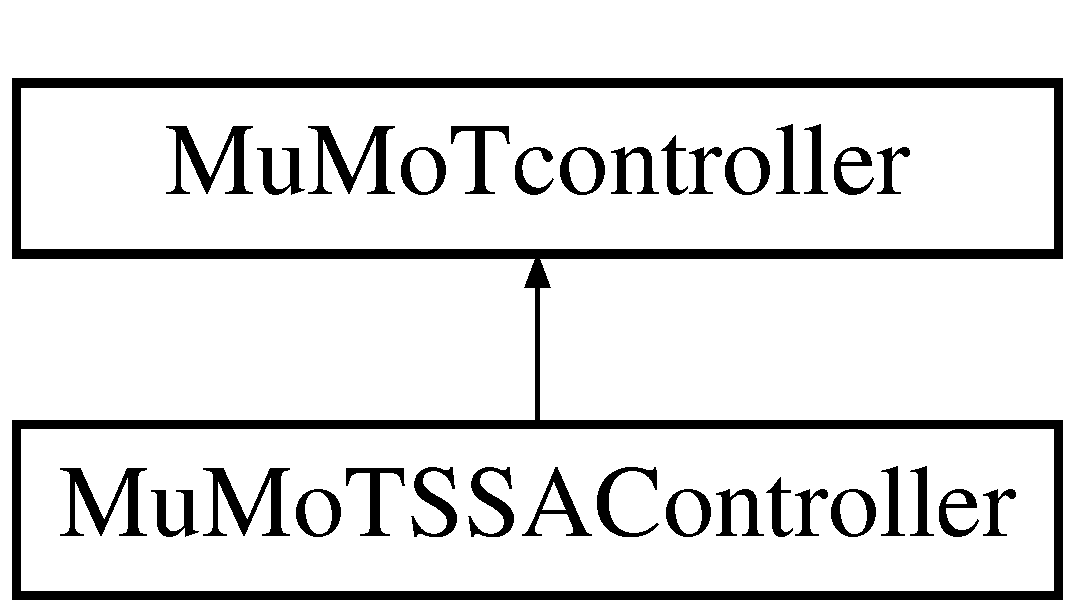
\includegraphics[height=2.000000cm]{class_mu_mo_t_1_1_mu_mo_t_1_1_mu_mo_t_s_s_a_controller}
\end{center}
\end{figure}
\subsection*{Public Member Functions}
\begin{DoxyCompactItemize}
\item 
def \hyperlink{class_mu_mo_t_1_1_mu_mo_t_1_1_mu_mo_t_s_s_a_controller_aca0478525092b12bd60e9ee971100a57}{\+\_\+\+\_\+init\+\_\+\+\_\+} (self, param\+Values, param\+Names, param\+Label\+Dict, continuous\+Replot, ssa\+Params, kwargs)
\end{DoxyCompactItemize}
\subsection*{Private Attributes}
\begin{DoxyCompactItemize}
\item 
\hyperlink{class_mu_mo_t_1_1_mu_mo_t_1_1_mu_mo_t_s_s_a_controller_a018864aa22d2adb0d3958fb0adbce8e2}{\+\_\+progress\+Bar}
\begin{DoxyCompactList}\small\item\em Toggle buttons for plotting style. \end{DoxyCompactList}\end{DoxyCompactItemize}
\subsection*{Additional Inherited Members}


\subsection{Detailed Description}
class describing a controller for multiagent views 

\subsection{Constructor \& Destructor Documentation}
\mbox{\Hypertarget{class_mu_mo_t_1_1_mu_mo_t_1_1_mu_mo_t_s_s_a_controller_aca0478525092b12bd60e9ee971100a57}\label{class_mu_mo_t_1_1_mu_mo_t_1_1_mu_mo_t_s_s_a_controller_aca0478525092b12bd60e9ee971100a57}} 
\index{Mu\+Mo\+T\+::\+Mu\+Mo\+T\+::\+Mu\+Mo\+T\+S\+S\+A\+Controller@{Mu\+Mo\+T\+::\+Mu\+Mo\+T\+::\+Mu\+Mo\+T\+S\+S\+A\+Controller}!\+\_\+\+\_\+init\+\_\+\+\_\+@{\+\_\+\+\_\+init\+\_\+\+\_\+}}
\index{\+\_\+\+\_\+init\+\_\+\+\_\+@{\+\_\+\+\_\+init\+\_\+\+\_\+}!Mu\+Mo\+T\+::\+Mu\+Mo\+T\+::\+Mu\+Mo\+T\+S\+S\+A\+Controller@{Mu\+Mo\+T\+::\+Mu\+Mo\+T\+::\+Mu\+Mo\+T\+S\+S\+A\+Controller}}
\subsubsection{\texorpdfstring{\+\_\+\+\_\+init\+\_\+\+\_\+()}{\_\_init\_\_()}}
{\footnotesize\ttfamily def \+\_\+\+\_\+init\+\_\+\+\_\+ (\begin{DoxyParamCaption}\item[{}]{self,  }\item[{}]{param\+Values,  }\item[{}]{param\+Names,  }\item[{}]{param\+Label\+Dict,  }\item[{}]{continuous\+Replot,  }\item[{}]{ssa\+Params,  }\item[{}]{kwargs }\end{DoxyParamCaption})}



\subsection{Field Documentation}
\mbox{\Hypertarget{class_mu_mo_t_1_1_mu_mo_t_1_1_mu_mo_t_s_s_a_controller_a018864aa22d2adb0d3958fb0adbce8e2}\label{class_mu_mo_t_1_1_mu_mo_t_1_1_mu_mo_t_s_s_a_controller_a018864aa22d2adb0d3958fb0adbce8e2}} 
\index{Mu\+Mo\+T\+::\+Mu\+Mo\+T\+::\+Mu\+Mo\+T\+S\+S\+A\+Controller@{Mu\+Mo\+T\+::\+Mu\+Mo\+T\+::\+Mu\+Mo\+T\+S\+S\+A\+Controller}!\+\_\+progress\+Bar@{\+\_\+progress\+Bar}}
\index{\+\_\+progress\+Bar@{\+\_\+progress\+Bar}!Mu\+Mo\+T\+::\+Mu\+Mo\+T\+::\+Mu\+Mo\+T\+S\+S\+A\+Controller@{Mu\+Mo\+T\+::\+Mu\+Mo\+T\+::\+Mu\+Mo\+T\+S\+S\+A\+Controller}}
\subsubsection{\texorpdfstring{\+\_\+progress\+Bar}{\_progressBar}}
{\footnotesize\ttfamily \+\_\+progress\+Bar\hspace{0.3cm}{\ttfamily [private]}}



Toggle buttons for plotting style. 

Checkbox for realtime plot update 

The documentation for this class was generated from the following file\+:\begin{DoxyCompactItemize}
\item 
Mu\+Mo\+T/\hyperlink{_mu_mo_t_8py}{Mu\+Mo\+T.\+py}\end{DoxyCompactItemize}

\hypertarget{class_mu_mo_t_1_1_mu_mo_t_1_1_mu_mo_t_s_s_a_view}{}\section{Mu\+Mo\+T\+S\+S\+A\+View Class Reference}
\label{class_mu_mo_t_1_1_mu_mo_t_1_1_mu_mo_t_s_s_a_view}\index{Mu\+Mo\+T\+S\+S\+A\+View@{Mu\+Mo\+T\+S\+S\+A\+View}}


agent on networks view on model  


Inheritance diagram for Mu\+Mo\+T\+S\+S\+A\+View\+:\begin{figure}[H]
\begin{center}
\leavevmode
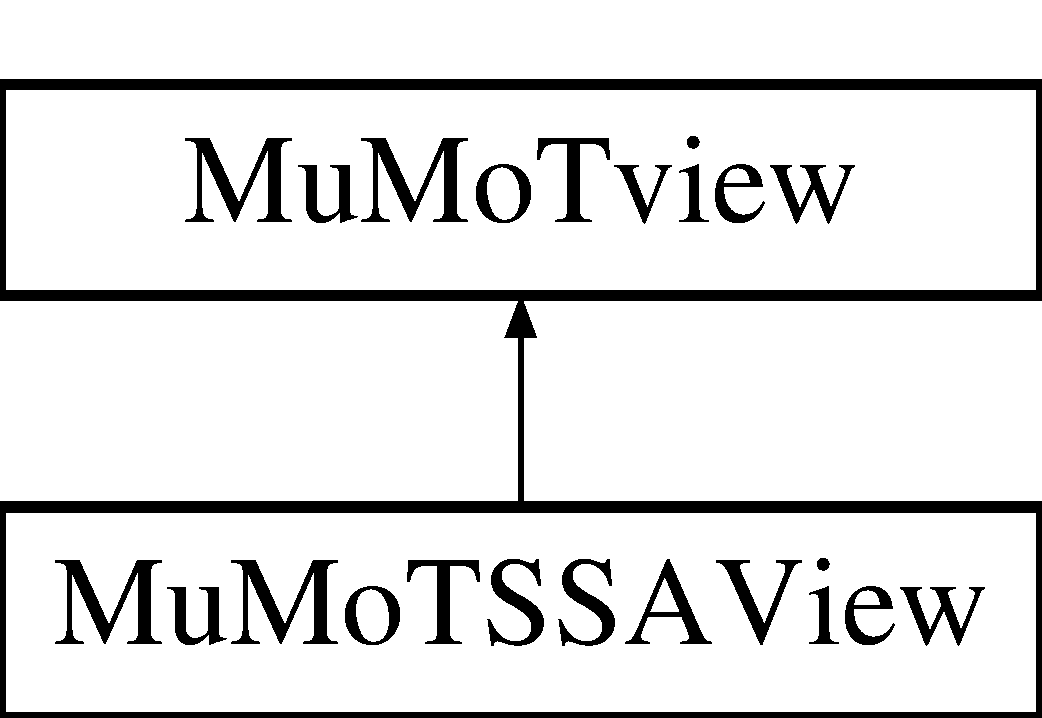
\includegraphics[height=2.000000cm]{class_mu_mo_t_1_1_mu_mo_t_1_1_mu_mo_t_s_s_a_view}
\end{center}
\end{figure}
\subsection*{Public Member Functions}
\begin{DoxyCompactItemize}
\item 
def \hyperlink{class_mu_mo_t_1_1_mu_mo_t_1_1_mu_mo_t_s_s_a_view_ae0e9bcf60ca39799461bccf0e672c323}{\+\_\+\+\_\+init\+\_\+\+\_\+} (self, model, controller, ssa\+Params, figure=None, rates=None, kwargs)
\end{DoxyCompactItemize}
\subsection*{Private Member Functions}
\begin{DoxyCompactItemize}
\item 
def \hyperlink{class_mu_mo_t_1_1_mu_mo_t_1_1_mu_mo_t_s_s_a_view_a47b00aaebcccf3c8dc2183a406404349}{\+\_\+update\+\_\+params} (self)
\item 
def \hyperlink{class_mu_mo_t_1_1_mu_mo_t_1_1_mu_mo_t_s_s_a_view_a3af54c33f997937b14f422e772d5280a}{\+\_\+print\+\_\+standalone\+\_\+view\+\_\+cmd} (self)
\item 
def \hyperlink{class_mu_mo_t_1_1_mu_mo_t_1_1_mu_mo_t_s_s_a_view_a57cea7fd9ea5c1805b9c18fc4b0adc0b}{\+\_\+redraw\+Only} (self)
\item 
def \hyperlink{class_mu_mo_t_1_1_mu_mo_t_1_1_mu_mo_t_s_s_a_view_ace35072dcd3e51e67107f62b4de0d5fe}{\+\_\+plot\+\_\+time\+Evolution} (self)
\item 
def \hyperlink{class_mu_mo_t_1_1_mu_mo_t_1_1_mu_mo_t_s_s_a_view_ab4e39bf1c45dbb1f9b6a6a5352de4d8f}{\+\_\+run\+S\+SA} (self)
\item 
def \hyperlink{class_mu_mo_t_1_1_mu_mo_t_1_1_mu_mo_t_s_s_a_view_a054aa0e8c130babbca21a6ff0e0fd31a}{\+\_\+init\+Figure} (self)
\item 
def \hyperlink{class_mu_mo_t_1_1_mu_mo_t_1_1_mu_mo_t_s_s_a_view_aae445216655e4d91f9b386249daf1541}{\+\_\+update\+S\+S\+A\+Figure} (self, evo, full\+Plot=True)
\item 
def \hyperlink{class_mu_mo_t_1_1_mu_mo_t_1_1_mu_mo_t_s_s_a_view_ac3f09eae4152f838b1693edc4203ee67}{\+\_\+create\+S\+S\+Amatrix} (self)
\item 
def \hyperlink{class_mu_mo_t_1_1_mu_mo_t_1_1_mu_mo_t_s_s_a_view_a1d2f8bb3e67d82bd01a95d58220d099b}{\+\_\+step\+S\+SA} (self, current\+State)
\item 
def \hyperlink{class_mu_mo_t_1_1_mu_mo_t_1_1_mu_mo_t_s_s_a_view_a51d421aacb4cd83af5f1c2e60c3dff9c}{\+\_\+single\+Run} (self, random\+Seed)
\end{DoxyCompactItemize}
\subsection*{Private Attributes}
\begin{DoxyCompactItemize}
\item 
\hyperlink{class_mu_mo_t_1_1_mu_mo_t_1_1_mu_mo_t_s_s_a_view_a15f56ca9811d1e67d721fa64f9b0dc1e}{\+\_\+controller}
\end{DoxyCompactItemize}
\subsection*{Static Private Attributes}
\begin{DoxyCompactItemize}
\item 
\hyperlink{class_mu_mo_t_1_1_mu_mo_t_1_1_mu_mo_t_s_s_a_view_a6aaed74c935ed5380691798f75527a18}{\+\_\+colors} = None
\item 
\hyperlink{class_mu_mo_t_1_1_mu_mo_t_1_1_mu_mo_t_s_s_a_view_a2fc08b0021064bc60e2a9349157357bc}{\+\_\+reactants\+Matrix} = None
\begin{DoxyCompactList}\small\item\em a matrix form of the left-\/handside of the rules \end{DoxyCompactList}\item 
\hyperlink{class_mu_mo_t_1_1_mu_mo_t_1_1_mu_mo_t_s_s_a_view_a6a882ef2523ac168ac8a5c87e78b8ed0}{\+\_\+rule\+Changes} = None
\begin{DoxyCompactList}\small\item\em the effect of each rule \end{DoxyCompactList}\item 
\hyperlink{class_mu_mo_t_1_1_mu_mo_t_1_1_mu_mo_t_s_s_a_view_a8afeb8cf5705c6b521f7d6658dab955b}{\+\_\+initial\+State} = None
\begin{DoxyCompactList}\small\item\em the system state at the start of the simulation (timestep zero) \end{DoxyCompactList}\item 
\hyperlink{class_mu_mo_t_1_1_mu_mo_t_1_1_mu_mo_t_s_s_a_view_a7c4303b3e2a8784a0cc16cd523069203}{\+\_\+rates\+Dict} = None
\begin{DoxyCompactList}\small\item\em dictionary of rates \end{DoxyCompactList}\item 
\hyperlink{class_mu_mo_t_1_1_mu_mo_t_1_1_mu_mo_t_s_s_a_view_a956572b83e957005ef90a30995891585}{\+\_\+max\+Time} = None
\begin{DoxyCompactList}\small\item\em number of simulation timesteps \end{DoxyCompactList}\item 
\hyperlink{class_mu_mo_t_1_1_mu_mo_t_1_1_mu_mo_t_s_s_a_view_a79e90c970112c845893400f85a2590dd}{\+\_\+random\+Seed} = None
\begin{DoxyCompactList}\small\item\em random seed \end{DoxyCompactList}\item 
\hyperlink{class_mu_mo_t_1_1_mu_mo_t_1_1_mu_mo_t_s_s_a_view_ae8c8d7969b8ab8f31df9d1d1d10eabb9}{\+\_\+visualisation\+Type} = None
\begin{DoxyCompactList}\small\item\em visualisation type \end{DoxyCompactList}\item 
\hyperlink{class_mu_mo_t_1_1_mu_mo_t_1_1_mu_mo_t_s_s_a_view_a194d04e5fee40987d78aa7e1f721ea28}{\+\_\+realtime\+Plot} = None
\begin{DoxyCompactList}\small\item\em realtime\+Plot flag (T\+R\+UE = the plot is updated each timestep of the simulation; F\+A\+L\+SE = it is updated once at the end of the simulation) \end{DoxyCompactList}\item 
\hyperlink{class_mu_mo_t_1_1_mu_mo_t_1_1_mu_mo_t_s_s_a_view_a8da8c49a2b0ccc518cf7f333bdbd17a6}{\+\_\+latest\+Results} = None
\begin{DoxyCompactList}\small\item\em latest computed results \end{DoxyCompactList}\end{DoxyCompactItemize}
\subsection*{Additional Inherited Members}


\subsection{Detailed Description}
agent on networks view on model 

\subsection{Constructor \& Destructor Documentation}
\mbox{\Hypertarget{class_mu_mo_t_1_1_mu_mo_t_1_1_mu_mo_t_s_s_a_view_ae0e9bcf60ca39799461bccf0e672c323}\label{class_mu_mo_t_1_1_mu_mo_t_1_1_mu_mo_t_s_s_a_view_ae0e9bcf60ca39799461bccf0e672c323}} 
\index{Mu\+Mo\+T\+::\+Mu\+Mo\+T\+::\+Mu\+Mo\+T\+S\+S\+A\+View@{Mu\+Mo\+T\+::\+Mu\+Mo\+T\+::\+Mu\+Mo\+T\+S\+S\+A\+View}!\+\_\+\+\_\+init\+\_\+\+\_\+@{\+\_\+\+\_\+init\+\_\+\+\_\+}}
\index{\+\_\+\+\_\+init\+\_\+\+\_\+@{\+\_\+\+\_\+init\+\_\+\+\_\+}!Mu\+Mo\+T\+::\+Mu\+Mo\+T\+::\+Mu\+Mo\+T\+S\+S\+A\+View@{Mu\+Mo\+T\+::\+Mu\+Mo\+T\+::\+Mu\+Mo\+T\+S\+S\+A\+View}}
\subsubsection{\texorpdfstring{\+\_\+\+\_\+init\+\_\+\+\_\+()}{\_\_init\_\_()}}
{\footnotesize\ttfamily def \+\_\+\+\_\+init\+\_\+\+\_\+ (\begin{DoxyParamCaption}\item[{}]{self,  }\item[{}]{model,  }\item[{}]{controller,  }\item[{}]{ssa\+Params,  }\item[{}]{figure = {\ttfamily None},  }\item[{}]{rates = {\ttfamily None},  }\item[{}]{kwargs }\end{DoxyParamCaption})}



\subsection{Member Function Documentation}
\mbox{\Hypertarget{class_mu_mo_t_1_1_mu_mo_t_1_1_mu_mo_t_s_s_a_view_ac3f09eae4152f838b1693edc4203ee67}\label{class_mu_mo_t_1_1_mu_mo_t_1_1_mu_mo_t_s_s_a_view_ac3f09eae4152f838b1693edc4203ee67}} 
\index{Mu\+Mo\+T\+::\+Mu\+Mo\+T\+::\+Mu\+Mo\+T\+S\+S\+A\+View@{Mu\+Mo\+T\+::\+Mu\+Mo\+T\+::\+Mu\+Mo\+T\+S\+S\+A\+View}!\+\_\+create\+S\+S\+Amatrix@{\+\_\+create\+S\+S\+Amatrix}}
\index{\+\_\+create\+S\+S\+Amatrix@{\+\_\+create\+S\+S\+Amatrix}!Mu\+Mo\+T\+::\+Mu\+Mo\+T\+::\+Mu\+Mo\+T\+S\+S\+A\+View@{Mu\+Mo\+T\+::\+Mu\+Mo\+T\+::\+Mu\+Mo\+T\+S\+S\+A\+View}}
\subsubsection{\texorpdfstring{\+\_\+create\+S\+S\+Amatrix()}{\_createSSAmatrix()}}
{\footnotesize\ttfamily def \+\_\+create\+S\+S\+Amatrix (\begin{DoxyParamCaption}\item[{}]{self }\end{DoxyParamCaption})\hspace{0.3cm}{\ttfamily [private]}}

\begin{DoxyRefDesc}{Todo}
\item[\hyperlink{todo__todo000064}{Todo}]Deprecated method to be removed \end{DoxyRefDesc}
\mbox{\Hypertarget{class_mu_mo_t_1_1_mu_mo_t_1_1_mu_mo_t_s_s_a_view_a054aa0e8c130babbca21a6ff0e0fd31a}\label{class_mu_mo_t_1_1_mu_mo_t_1_1_mu_mo_t_s_s_a_view_a054aa0e8c130babbca21a6ff0e0fd31a}} 
\index{Mu\+Mo\+T\+::\+Mu\+Mo\+T\+::\+Mu\+Mo\+T\+S\+S\+A\+View@{Mu\+Mo\+T\+::\+Mu\+Mo\+T\+::\+Mu\+Mo\+T\+S\+S\+A\+View}!\+\_\+init\+Figure@{\+\_\+init\+Figure}}
\index{\+\_\+init\+Figure@{\+\_\+init\+Figure}!Mu\+Mo\+T\+::\+Mu\+Mo\+T\+::\+Mu\+Mo\+T\+S\+S\+A\+View@{Mu\+Mo\+T\+::\+Mu\+Mo\+T\+::\+Mu\+Mo\+T\+S\+S\+A\+View}}
\subsubsection{\texorpdfstring{\+\_\+init\+Figure()}{\_initFigure()}}
{\footnotesize\ttfamily def \+\_\+init\+Figure (\begin{DoxyParamCaption}\item[{}]{self }\end{DoxyParamCaption})\hspace{0.3cm}{\ttfamily [private]}}

\mbox{\Hypertarget{class_mu_mo_t_1_1_mu_mo_t_1_1_mu_mo_t_s_s_a_view_ace35072dcd3e51e67107f62b4de0d5fe}\label{class_mu_mo_t_1_1_mu_mo_t_1_1_mu_mo_t_s_s_a_view_ace35072dcd3e51e67107f62b4de0d5fe}} 
\index{Mu\+Mo\+T\+::\+Mu\+Mo\+T\+::\+Mu\+Mo\+T\+S\+S\+A\+View@{Mu\+Mo\+T\+::\+Mu\+Mo\+T\+::\+Mu\+Mo\+T\+S\+S\+A\+View}!\+\_\+plot\+\_\+time\+Evolution@{\+\_\+plot\+\_\+time\+Evolution}}
\index{\+\_\+plot\+\_\+time\+Evolution@{\+\_\+plot\+\_\+time\+Evolution}!Mu\+Mo\+T\+::\+Mu\+Mo\+T\+::\+Mu\+Mo\+T\+S\+S\+A\+View@{Mu\+Mo\+T\+::\+Mu\+Mo\+T\+::\+Mu\+Mo\+T\+S\+S\+A\+View}}
\subsubsection{\texorpdfstring{\+\_\+plot\+\_\+time\+Evolution()}{\_plot\_timeEvolution()}}
{\footnotesize\ttfamily def \+\_\+plot\+\_\+time\+Evolution (\begin{DoxyParamCaption}\item[{}]{self }\end{DoxyParamCaption})\hspace{0.3cm}{\ttfamily [private]}}

\mbox{\Hypertarget{class_mu_mo_t_1_1_mu_mo_t_1_1_mu_mo_t_s_s_a_view_a3af54c33f997937b14f422e772d5280a}\label{class_mu_mo_t_1_1_mu_mo_t_1_1_mu_mo_t_s_s_a_view_a3af54c33f997937b14f422e772d5280a}} 
\index{Mu\+Mo\+T\+::\+Mu\+Mo\+T\+::\+Mu\+Mo\+T\+S\+S\+A\+View@{Mu\+Mo\+T\+::\+Mu\+Mo\+T\+::\+Mu\+Mo\+T\+S\+S\+A\+View}!\+\_\+print\+\_\+standalone\+\_\+view\+\_\+cmd@{\+\_\+print\+\_\+standalone\+\_\+view\+\_\+cmd}}
\index{\+\_\+print\+\_\+standalone\+\_\+view\+\_\+cmd@{\+\_\+print\+\_\+standalone\+\_\+view\+\_\+cmd}!Mu\+Mo\+T\+::\+Mu\+Mo\+T\+::\+Mu\+Mo\+T\+S\+S\+A\+View@{Mu\+Mo\+T\+::\+Mu\+Mo\+T\+::\+Mu\+Mo\+T\+S\+S\+A\+View}}
\subsubsection{\texorpdfstring{\+\_\+print\+\_\+standalone\+\_\+view\+\_\+cmd()}{\_print\_standalone\_view\_cmd()}}
{\footnotesize\ttfamily def \+\_\+print\+\_\+standalone\+\_\+view\+\_\+cmd (\begin{DoxyParamCaption}\item[{}]{self }\end{DoxyParamCaption})\hspace{0.3cm}{\ttfamily [private]}}

\mbox{\Hypertarget{class_mu_mo_t_1_1_mu_mo_t_1_1_mu_mo_t_s_s_a_view_a57cea7fd9ea5c1805b9c18fc4b0adc0b}\label{class_mu_mo_t_1_1_mu_mo_t_1_1_mu_mo_t_s_s_a_view_a57cea7fd9ea5c1805b9c18fc4b0adc0b}} 
\index{Mu\+Mo\+T\+::\+Mu\+Mo\+T\+::\+Mu\+Mo\+T\+S\+S\+A\+View@{Mu\+Mo\+T\+::\+Mu\+Mo\+T\+::\+Mu\+Mo\+T\+S\+S\+A\+View}!\+\_\+redraw\+Only@{\+\_\+redraw\+Only}}
\index{\+\_\+redraw\+Only@{\+\_\+redraw\+Only}!Mu\+Mo\+T\+::\+Mu\+Mo\+T\+::\+Mu\+Mo\+T\+S\+S\+A\+View@{Mu\+Mo\+T\+::\+Mu\+Mo\+T\+::\+Mu\+Mo\+T\+S\+S\+A\+View}}
\subsubsection{\texorpdfstring{\+\_\+redraw\+Only()}{\_redrawOnly()}}
{\footnotesize\ttfamily def \+\_\+redraw\+Only (\begin{DoxyParamCaption}\item[{}]{self }\end{DoxyParamCaption})\hspace{0.3cm}{\ttfamily [private]}}

\mbox{\Hypertarget{class_mu_mo_t_1_1_mu_mo_t_1_1_mu_mo_t_s_s_a_view_ab4e39bf1c45dbb1f9b6a6a5352de4d8f}\label{class_mu_mo_t_1_1_mu_mo_t_1_1_mu_mo_t_s_s_a_view_ab4e39bf1c45dbb1f9b6a6a5352de4d8f}} 
\index{Mu\+Mo\+T\+::\+Mu\+Mo\+T\+::\+Mu\+Mo\+T\+S\+S\+A\+View@{Mu\+Mo\+T\+::\+Mu\+Mo\+T\+::\+Mu\+Mo\+T\+S\+S\+A\+View}!\+\_\+run\+S\+SA@{\+\_\+run\+S\+SA}}
\index{\+\_\+run\+S\+SA@{\+\_\+run\+S\+SA}!Mu\+Mo\+T\+::\+Mu\+Mo\+T\+::\+Mu\+Mo\+T\+S\+S\+A\+View@{Mu\+Mo\+T\+::\+Mu\+Mo\+T\+::\+Mu\+Mo\+T\+S\+S\+A\+View}}
\subsubsection{\texorpdfstring{\+\_\+run\+S\+S\+A()}{\_runSSA()}}
{\footnotesize\ttfamily def \+\_\+run\+S\+SA (\begin{DoxyParamCaption}\item[{}]{self }\end{DoxyParamCaption})\hspace{0.3cm}{\ttfamily [private]}}

\mbox{\Hypertarget{class_mu_mo_t_1_1_mu_mo_t_1_1_mu_mo_t_s_s_a_view_a51d421aacb4cd83af5f1c2e60c3dff9c}\label{class_mu_mo_t_1_1_mu_mo_t_1_1_mu_mo_t_s_s_a_view_a51d421aacb4cd83af5f1c2e60c3dff9c}} 
\index{Mu\+Mo\+T\+::\+Mu\+Mo\+T\+::\+Mu\+Mo\+T\+S\+S\+A\+View@{Mu\+Mo\+T\+::\+Mu\+Mo\+T\+::\+Mu\+Mo\+T\+S\+S\+A\+View}!\+\_\+single\+Run@{\+\_\+single\+Run}}
\index{\+\_\+single\+Run@{\+\_\+single\+Run}!Mu\+Mo\+T\+::\+Mu\+Mo\+T\+::\+Mu\+Mo\+T\+S\+S\+A\+View@{Mu\+Mo\+T\+::\+Mu\+Mo\+T\+::\+Mu\+Mo\+T\+S\+S\+A\+View}}
\subsubsection{\texorpdfstring{\+\_\+single\+Run()}{\_singleRun()}}
{\footnotesize\ttfamily def \+\_\+single\+Run (\begin{DoxyParamCaption}\item[{}]{self,  }\item[{}]{random\+Seed }\end{DoxyParamCaption})\hspace{0.3cm}{\ttfamily [private]}}

\begin{DoxyRefDesc}{Todo}
\item[\hyperlink{todo__todo000065}{Todo}]check if it is still running correctly after structural change for View independence from Controller (especially, if initial\+State is correctly initialised) \end{DoxyRefDesc}
\mbox{\Hypertarget{class_mu_mo_t_1_1_mu_mo_t_1_1_mu_mo_t_s_s_a_view_a1d2f8bb3e67d82bd01a95d58220d099b}\label{class_mu_mo_t_1_1_mu_mo_t_1_1_mu_mo_t_s_s_a_view_a1d2f8bb3e67d82bd01a95d58220d099b}} 
\index{Mu\+Mo\+T\+::\+Mu\+Mo\+T\+::\+Mu\+Mo\+T\+S\+S\+A\+View@{Mu\+Mo\+T\+::\+Mu\+Mo\+T\+::\+Mu\+Mo\+T\+S\+S\+A\+View}!\+\_\+step\+S\+SA@{\+\_\+step\+S\+SA}}
\index{\+\_\+step\+S\+SA@{\+\_\+step\+S\+SA}!Mu\+Mo\+T\+::\+Mu\+Mo\+T\+::\+Mu\+Mo\+T\+S\+S\+A\+View@{Mu\+Mo\+T\+::\+Mu\+Mo\+T\+::\+Mu\+Mo\+T\+S\+S\+A\+View}}
\subsubsection{\texorpdfstring{\+\_\+step\+S\+S\+A()}{\_stepSSA()}}
{\footnotesize\ttfamily def \+\_\+step\+S\+SA (\begin{DoxyParamCaption}\item[{}]{self,  }\item[{}]{current\+State }\end{DoxyParamCaption})\hspace{0.3cm}{\ttfamily [private]}}

\mbox{\Hypertarget{class_mu_mo_t_1_1_mu_mo_t_1_1_mu_mo_t_s_s_a_view_a47b00aaebcccf3c8dc2183a406404349}\label{class_mu_mo_t_1_1_mu_mo_t_1_1_mu_mo_t_s_s_a_view_a47b00aaebcccf3c8dc2183a406404349}} 
\index{Mu\+Mo\+T\+::\+Mu\+Mo\+T\+::\+Mu\+Mo\+T\+S\+S\+A\+View@{Mu\+Mo\+T\+::\+Mu\+Mo\+T\+::\+Mu\+Mo\+T\+S\+S\+A\+View}!\+\_\+update\+\_\+params@{\+\_\+update\+\_\+params}}
\index{\+\_\+update\+\_\+params@{\+\_\+update\+\_\+params}!Mu\+Mo\+T\+::\+Mu\+Mo\+T\+::\+Mu\+Mo\+T\+S\+S\+A\+View@{Mu\+Mo\+T\+::\+Mu\+Mo\+T\+::\+Mu\+Mo\+T\+S\+S\+A\+View}}
\subsubsection{\texorpdfstring{\+\_\+update\+\_\+params()}{\_update\_params()}}
{\footnotesize\ttfamily def \+\_\+update\+\_\+params (\begin{DoxyParamCaption}\item[{}]{self }\end{DoxyParamCaption})\hspace{0.3cm}{\ttfamily [private]}}

\mbox{\Hypertarget{class_mu_mo_t_1_1_mu_mo_t_1_1_mu_mo_t_s_s_a_view_aae445216655e4d91f9b386249daf1541}\label{class_mu_mo_t_1_1_mu_mo_t_1_1_mu_mo_t_s_s_a_view_aae445216655e4d91f9b386249daf1541}} 
\index{Mu\+Mo\+T\+::\+Mu\+Mo\+T\+::\+Mu\+Mo\+T\+S\+S\+A\+View@{Mu\+Mo\+T\+::\+Mu\+Mo\+T\+::\+Mu\+Mo\+T\+S\+S\+A\+View}!\+\_\+update\+S\+S\+A\+Figure@{\+\_\+update\+S\+S\+A\+Figure}}
\index{\+\_\+update\+S\+S\+A\+Figure@{\+\_\+update\+S\+S\+A\+Figure}!Mu\+Mo\+T\+::\+Mu\+Mo\+T\+::\+Mu\+Mo\+T\+S\+S\+A\+View@{Mu\+Mo\+T\+::\+Mu\+Mo\+T\+::\+Mu\+Mo\+T\+S\+S\+A\+View}}
\subsubsection{\texorpdfstring{\+\_\+update\+S\+S\+A\+Figure()}{\_updateSSAFigure()}}
{\footnotesize\ttfamily def \+\_\+update\+S\+S\+A\+Figure (\begin{DoxyParamCaption}\item[{}]{self,  }\item[{}]{evo,  }\item[{}]{full\+Plot = {\ttfamily True} }\end{DoxyParamCaption})\hspace{0.3cm}{\ttfamily [private]}}



\subsection{Field Documentation}
\mbox{\Hypertarget{class_mu_mo_t_1_1_mu_mo_t_1_1_mu_mo_t_s_s_a_view_a6aaed74c935ed5380691798f75527a18}\label{class_mu_mo_t_1_1_mu_mo_t_1_1_mu_mo_t_s_s_a_view_a6aaed74c935ed5380691798f75527a18}} 
\index{Mu\+Mo\+T\+::\+Mu\+Mo\+T\+::\+Mu\+Mo\+T\+S\+S\+A\+View@{Mu\+Mo\+T\+::\+Mu\+Mo\+T\+::\+Mu\+Mo\+T\+S\+S\+A\+View}!\+\_\+colors@{\+\_\+colors}}
\index{\+\_\+colors@{\+\_\+colors}!Mu\+Mo\+T\+::\+Mu\+Mo\+T\+::\+Mu\+Mo\+T\+S\+S\+A\+View@{Mu\+Mo\+T\+::\+Mu\+Mo\+T\+::\+Mu\+Mo\+T\+S\+S\+A\+View}}
\subsubsection{\texorpdfstring{\+\_\+colors}{\_colors}}
{\footnotesize\ttfamily \+\_\+colors = None\hspace{0.3cm}{\ttfamily [static]}, {\ttfamily [private]}}

\mbox{\Hypertarget{class_mu_mo_t_1_1_mu_mo_t_1_1_mu_mo_t_s_s_a_view_a15f56ca9811d1e67d721fa64f9b0dc1e}\label{class_mu_mo_t_1_1_mu_mo_t_1_1_mu_mo_t_s_s_a_view_a15f56ca9811d1e67d721fa64f9b0dc1e}} 
\index{Mu\+Mo\+T\+::\+Mu\+Mo\+T\+::\+Mu\+Mo\+T\+S\+S\+A\+View@{Mu\+Mo\+T\+::\+Mu\+Mo\+T\+::\+Mu\+Mo\+T\+S\+S\+A\+View}!\+\_\+controller@{\+\_\+controller}}
\index{\+\_\+controller@{\+\_\+controller}!Mu\+Mo\+T\+::\+Mu\+Mo\+T\+::\+Mu\+Mo\+T\+S\+S\+A\+View@{Mu\+Mo\+T\+::\+Mu\+Mo\+T\+::\+Mu\+Mo\+T\+S\+S\+A\+View}}
\subsubsection{\texorpdfstring{\+\_\+controller}{\_controller}}
{\footnotesize\ttfamily \+\_\+controller\hspace{0.3cm}{\ttfamily [private]}}

\mbox{\Hypertarget{class_mu_mo_t_1_1_mu_mo_t_1_1_mu_mo_t_s_s_a_view_a8afeb8cf5705c6b521f7d6658dab955b}\label{class_mu_mo_t_1_1_mu_mo_t_1_1_mu_mo_t_s_s_a_view_a8afeb8cf5705c6b521f7d6658dab955b}} 
\index{Mu\+Mo\+T\+::\+Mu\+Mo\+T\+::\+Mu\+Mo\+T\+S\+S\+A\+View@{Mu\+Mo\+T\+::\+Mu\+Mo\+T\+::\+Mu\+Mo\+T\+S\+S\+A\+View}!\+\_\+initial\+State@{\+\_\+initial\+State}}
\index{\+\_\+initial\+State@{\+\_\+initial\+State}!Mu\+Mo\+T\+::\+Mu\+Mo\+T\+::\+Mu\+Mo\+T\+S\+S\+A\+View@{Mu\+Mo\+T\+::\+Mu\+Mo\+T\+::\+Mu\+Mo\+T\+S\+S\+A\+View}}
\subsubsection{\texorpdfstring{\+\_\+initial\+State}{\_initialState}}
{\footnotesize\ttfamily \+\_\+initial\+State = None\hspace{0.3cm}{\ttfamily [static]}, {\ttfamily [private]}}



the system state at the start of the simulation (timestep zero) 

\mbox{\Hypertarget{class_mu_mo_t_1_1_mu_mo_t_1_1_mu_mo_t_s_s_a_view_a8da8c49a2b0ccc518cf7f333bdbd17a6}\label{class_mu_mo_t_1_1_mu_mo_t_1_1_mu_mo_t_s_s_a_view_a8da8c49a2b0ccc518cf7f333bdbd17a6}} 
\index{Mu\+Mo\+T\+::\+Mu\+Mo\+T\+::\+Mu\+Mo\+T\+S\+S\+A\+View@{Mu\+Mo\+T\+::\+Mu\+Mo\+T\+::\+Mu\+Mo\+T\+S\+S\+A\+View}!\+\_\+latest\+Results@{\+\_\+latest\+Results}}
\index{\+\_\+latest\+Results@{\+\_\+latest\+Results}!Mu\+Mo\+T\+::\+Mu\+Mo\+T\+::\+Mu\+Mo\+T\+S\+S\+A\+View@{Mu\+Mo\+T\+::\+Mu\+Mo\+T\+::\+Mu\+Mo\+T\+S\+S\+A\+View}}
\subsubsection{\texorpdfstring{\+\_\+latest\+Results}{\_latestResults}}
{\footnotesize\ttfamily \+\_\+latest\+Results = None\hspace{0.3cm}{\ttfamily [static]}, {\ttfamily [private]}}



latest computed results 

\mbox{\Hypertarget{class_mu_mo_t_1_1_mu_mo_t_1_1_mu_mo_t_s_s_a_view_a956572b83e957005ef90a30995891585}\label{class_mu_mo_t_1_1_mu_mo_t_1_1_mu_mo_t_s_s_a_view_a956572b83e957005ef90a30995891585}} 
\index{Mu\+Mo\+T\+::\+Mu\+Mo\+T\+::\+Mu\+Mo\+T\+S\+S\+A\+View@{Mu\+Mo\+T\+::\+Mu\+Mo\+T\+::\+Mu\+Mo\+T\+S\+S\+A\+View}!\+\_\+max\+Time@{\+\_\+max\+Time}}
\index{\+\_\+max\+Time@{\+\_\+max\+Time}!Mu\+Mo\+T\+::\+Mu\+Mo\+T\+::\+Mu\+Mo\+T\+S\+S\+A\+View@{Mu\+Mo\+T\+::\+Mu\+Mo\+T\+::\+Mu\+Mo\+T\+S\+S\+A\+View}}
\subsubsection{\texorpdfstring{\+\_\+max\+Time}{\_maxTime}}
{\footnotesize\ttfamily \+\_\+max\+Time = None\hspace{0.3cm}{\ttfamily [static]}, {\ttfamily [private]}}



number of simulation timesteps 

\mbox{\Hypertarget{class_mu_mo_t_1_1_mu_mo_t_1_1_mu_mo_t_s_s_a_view_a79e90c970112c845893400f85a2590dd}\label{class_mu_mo_t_1_1_mu_mo_t_1_1_mu_mo_t_s_s_a_view_a79e90c970112c845893400f85a2590dd}} 
\index{Mu\+Mo\+T\+::\+Mu\+Mo\+T\+::\+Mu\+Mo\+T\+S\+S\+A\+View@{Mu\+Mo\+T\+::\+Mu\+Mo\+T\+::\+Mu\+Mo\+T\+S\+S\+A\+View}!\+\_\+random\+Seed@{\+\_\+random\+Seed}}
\index{\+\_\+random\+Seed@{\+\_\+random\+Seed}!Mu\+Mo\+T\+::\+Mu\+Mo\+T\+::\+Mu\+Mo\+T\+S\+S\+A\+View@{Mu\+Mo\+T\+::\+Mu\+Mo\+T\+::\+Mu\+Mo\+T\+S\+S\+A\+View}}
\subsubsection{\texorpdfstring{\+\_\+random\+Seed}{\_randomSeed}}
{\footnotesize\ttfamily \+\_\+random\+Seed = None\hspace{0.3cm}{\ttfamily [static]}, {\ttfamily [private]}}



random seed 

\mbox{\Hypertarget{class_mu_mo_t_1_1_mu_mo_t_1_1_mu_mo_t_s_s_a_view_a7c4303b3e2a8784a0cc16cd523069203}\label{class_mu_mo_t_1_1_mu_mo_t_1_1_mu_mo_t_s_s_a_view_a7c4303b3e2a8784a0cc16cd523069203}} 
\index{Mu\+Mo\+T\+::\+Mu\+Mo\+T\+::\+Mu\+Mo\+T\+S\+S\+A\+View@{Mu\+Mo\+T\+::\+Mu\+Mo\+T\+::\+Mu\+Mo\+T\+S\+S\+A\+View}!\+\_\+rates\+Dict@{\+\_\+rates\+Dict}}
\index{\+\_\+rates\+Dict@{\+\_\+rates\+Dict}!Mu\+Mo\+T\+::\+Mu\+Mo\+T\+::\+Mu\+Mo\+T\+S\+S\+A\+View@{Mu\+Mo\+T\+::\+Mu\+Mo\+T\+::\+Mu\+Mo\+T\+S\+S\+A\+View}}
\subsubsection{\texorpdfstring{\+\_\+rates\+Dict}{\_ratesDict}}
{\footnotesize\ttfamily \+\_\+rates\+Dict = None\hspace{0.3cm}{\ttfamily [static]}, {\ttfamily [private]}}



dictionary of rates 

\begin{DoxyRefDesc}{Todo}
\item[\hyperlink{todo__todo000066}{Todo}]moving it to general method? \end{DoxyRefDesc}


\begin{DoxyRefDesc}{Todo}
\item[\hyperlink{todo__todo000067}{Todo}]moving it to general method? \end{DoxyRefDesc}
\mbox{\Hypertarget{class_mu_mo_t_1_1_mu_mo_t_1_1_mu_mo_t_s_s_a_view_a2fc08b0021064bc60e2a9349157357bc}\label{class_mu_mo_t_1_1_mu_mo_t_1_1_mu_mo_t_s_s_a_view_a2fc08b0021064bc60e2a9349157357bc}} 
\index{Mu\+Mo\+T\+::\+Mu\+Mo\+T\+::\+Mu\+Mo\+T\+S\+S\+A\+View@{Mu\+Mo\+T\+::\+Mu\+Mo\+T\+::\+Mu\+Mo\+T\+S\+S\+A\+View}!\+\_\+reactants\+Matrix@{\+\_\+reactants\+Matrix}}
\index{\+\_\+reactants\+Matrix@{\+\_\+reactants\+Matrix}!Mu\+Mo\+T\+::\+Mu\+Mo\+T\+::\+Mu\+Mo\+T\+S\+S\+A\+View@{Mu\+Mo\+T\+::\+Mu\+Mo\+T\+::\+Mu\+Mo\+T\+S\+S\+A\+View}}
\subsubsection{\texorpdfstring{\+\_\+reactants\+Matrix}{\_reactantsMatrix}}
{\footnotesize\ttfamily \+\_\+reactants\+Matrix = None\hspace{0.3cm}{\ttfamily [static]}, {\ttfamily [private]}}



a matrix form of the left-\/handside of the rules 

\mbox{\Hypertarget{class_mu_mo_t_1_1_mu_mo_t_1_1_mu_mo_t_s_s_a_view_a194d04e5fee40987d78aa7e1f721ea28}\label{class_mu_mo_t_1_1_mu_mo_t_1_1_mu_mo_t_s_s_a_view_a194d04e5fee40987d78aa7e1f721ea28}} 
\index{Mu\+Mo\+T\+::\+Mu\+Mo\+T\+::\+Mu\+Mo\+T\+S\+S\+A\+View@{Mu\+Mo\+T\+::\+Mu\+Mo\+T\+::\+Mu\+Mo\+T\+S\+S\+A\+View}!\+\_\+realtime\+Plot@{\+\_\+realtime\+Plot}}
\index{\+\_\+realtime\+Plot@{\+\_\+realtime\+Plot}!Mu\+Mo\+T\+::\+Mu\+Mo\+T\+::\+Mu\+Mo\+T\+S\+S\+A\+View@{Mu\+Mo\+T\+::\+Mu\+Mo\+T\+::\+Mu\+Mo\+T\+S\+S\+A\+View}}
\subsubsection{\texorpdfstring{\+\_\+realtime\+Plot}{\_realtimePlot}}
{\footnotesize\ttfamily \+\_\+realtime\+Plot = None\hspace{0.3cm}{\ttfamily [static]}, {\ttfamily [private]}}



realtime\+Plot flag (T\+R\+UE = the plot is updated each timestep of the simulation; F\+A\+L\+SE = it is updated once at the end of the simulation) 

\mbox{\Hypertarget{class_mu_mo_t_1_1_mu_mo_t_1_1_mu_mo_t_s_s_a_view_a6a882ef2523ac168ac8a5c87e78b8ed0}\label{class_mu_mo_t_1_1_mu_mo_t_1_1_mu_mo_t_s_s_a_view_a6a882ef2523ac168ac8a5c87e78b8ed0}} 
\index{Mu\+Mo\+T\+::\+Mu\+Mo\+T\+::\+Mu\+Mo\+T\+S\+S\+A\+View@{Mu\+Mo\+T\+::\+Mu\+Mo\+T\+::\+Mu\+Mo\+T\+S\+S\+A\+View}!\+\_\+rule\+Changes@{\+\_\+rule\+Changes}}
\index{\+\_\+rule\+Changes@{\+\_\+rule\+Changes}!Mu\+Mo\+T\+::\+Mu\+Mo\+T\+::\+Mu\+Mo\+T\+S\+S\+A\+View@{Mu\+Mo\+T\+::\+Mu\+Mo\+T\+::\+Mu\+Mo\+T\+S\+S\+A\+View}}
\subsubsection{\texorpdfstring{\+\_\+rule\+Changes}{\_ruleChanges}}
{\footnotesize\ttfamily \+\_\+rule\+Changes = None\hspace{0.3cm}{\ttfamily [static]}, {\ttfamily [private]}}



the effect of each rule 

\mbox{\Hypertarget{class_mu_mo_t_1_1_mu_mo_t_1_1_mu_mo_t_s_s_a_view_ae8c8d7969b8ab8f31df9d1d1d10eabb9}\label{class_mu_mo_t_1_1_mu_mo_t_1_1_mu_mo_t_s_s_a_view_ae8c8d7969b8ab8f31df9d1d1d10eabb9}} 
\index{Mu\+Mo\+T\+::\+Mu\+Mo\+T\+::\+Mu\+Mo\+T\+S\+S\+A\+View@{Mu\+Mo\+T\+::\+Mu\+Mo\+T\+::\+Mu\+Mo\+T\+S\+S\+A\+View}!\+\_\+visualisation\+Type@{\+\_\+visualisation\+Type}}
\index{\+\_\+visualisation\+Type@{\+\_\+visualisation\+Type}!Mu\+Mo\+T\+::\+Mu\+Mo\+T\+::\+Mu\+Mo\+T\+S\+S\+A\+View@{Mu\+Mo\+T\+::\+Mu\+Mo\+T\+::\+Mu\+Mo\+T\+S\+S\+A\+View}}
\subsubsection{\texorpdfstring{\+\_\+visualisation\+Type}{\_visualisationType}}
{\footnotesize\ttfamily \+\_\+visualisation\+Type = None\hspace{0.3cm}{\ttfamily [static]}, {\ttfamily [private]}}



visualisation type 

\begin{DoxyRefDesc}{Todo}
\item[\hyperlink{todo__todo000069}{Todo}]replot only the last part (rather than all the line) xdata.\+append( \mbox{[}i-\/1,i\mbox{]} ) pop = evo\mbox{[}state\mbox{]} ydata.\+append( pop\mbox{[}len(pop)-\/2\+:len(pop)\mbox{]} ) \end{DoxyRefDesc}


The documentation for this class was generated from the following file\+:\begin{DoxyCompactItemize}
\item 
Mu\+Mo\+T/\hyperlink{_mu_mo_t_8py}{Mu\+Mo\+T.\+py}\end{DoxyCompactItemize}

\hypertarget{class_mu_mo_t_1_1_mu_mo_t_1_1_mu_mo_tstream_view}{}\section{Mu\+Mo\+Tstream\+View Class Reference}
\label{class_mu_mo_t_1_1_mu_mo_t_1_1_mu_mo_tstream_view}\index{Mu\+Mo\+Tstream\+View@{Mu\+Mo\+Tstream\+View}}


stream plot view on model  


Inheritance diagram for Mu\+Mo\+Tstream\+View\+:\begin{figure}[H]
\begin{center}
\leavevmode
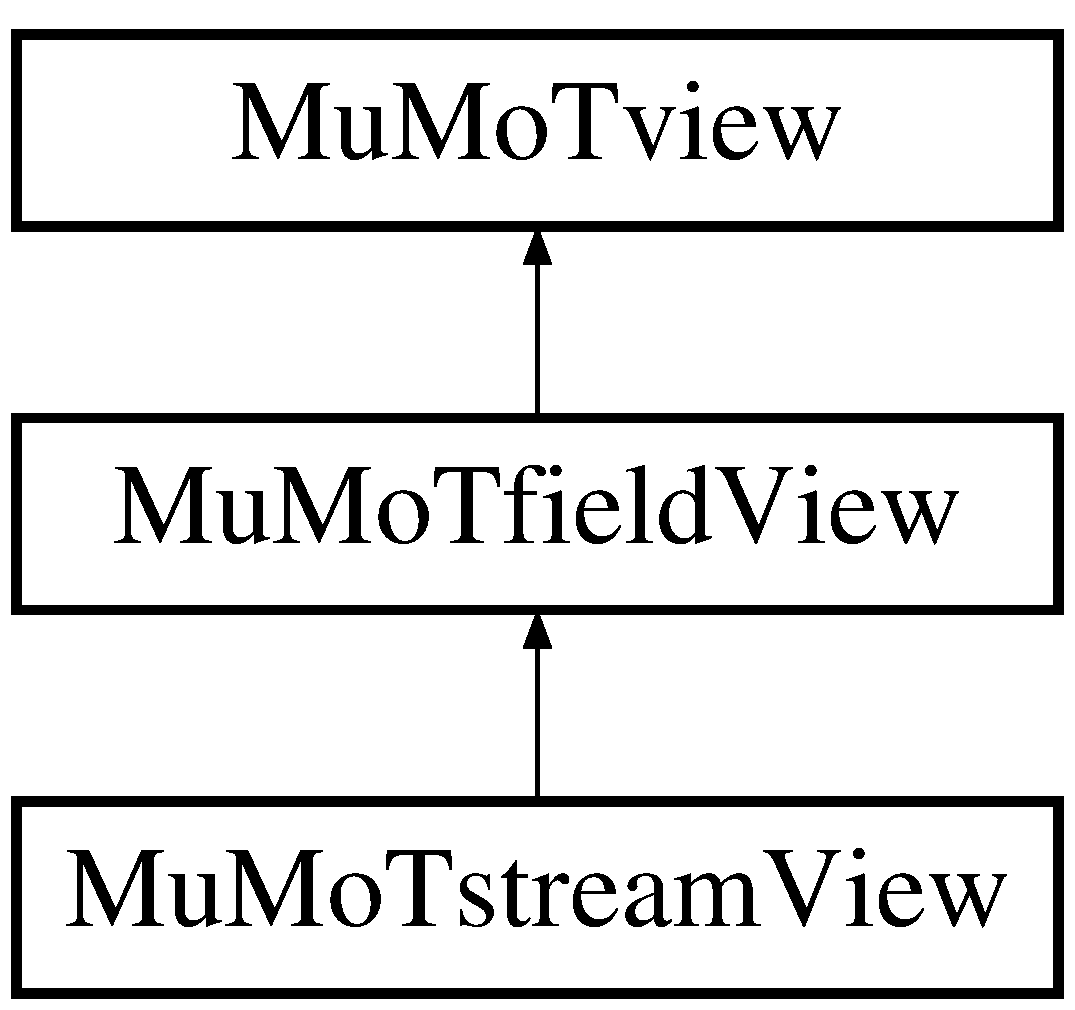
\includegraphics[height=3.000000cm]{class_mu_mo_t_1_1_mu_mo_t_1_1_mu_mo_tstream_view}
\end{center}
\end{figure}
\subsection*{Public Member Functions}
\begin{DoxyCompactItemize}
\item 
def \hyperlink{class_mu_mo_t_1_1_mu_mo_t_1_1_mu_mo_tstream_view_a302afe6819b093163cc8ea6f029c75da}{\+\_\+\+\_\+init\+\_\+\+\_\+} (self, args, kwargs)
\end{DoxyCompactItemize}
\subsection*{Private Member Functions}
\begin{DoxyCompactItemize}
\item 
def \hyperlink{class_mu_mo_t_1_1_mu_mo_t_1_1_mu_mo_tstream_view_a50d59419298116f738a98c864afb9d89}{\+\_\+plot\+\_\+field} (self)
\end{DoxyCompactItemize}
\subsection*{Private Attributes}
\begin{DoxyCompactItemize}
\item 
\hyperlink{class_mu_mo_t_1_1_mu_mo_t_1_1_mu_mo_tstream_view_ace48ed03490093d8f44cde91e2f1e86e}{\+\_\+generating\+Command}
\item 
\hyperlink{class_mu_mo_t_1_1_mu_mo_t_1_1_mu_mo_tstream_view_ac83a924ad62a2461d65b5c9bf9d27453}{\+\_\+show\+Fixed\+Points}
\end{DoxyCompactItemize}
\subsection*{Additional Inherited Members}


\subsection{Detailed Description}
stream plot view on model 

\subsection{Constructor \& Destructor Documentation}
\mbox{\Hypertarget{class_mu_mo_t_1_1_mu_mo_t_1_1_mu_mo_tstream_view_a302afe6819b093163cc8ea6f029c75da}\label{class_mu_mo_t_1_1_mu_mo_t_1_1_mu_mo_tstream_view_a302afe6819b093163cc8ea6f029c75da}} 
\index{Mu\+Mo\+T\+::\+Mu\+Mo\+T\+::\+Mu\+Mo\+Tstream\+View@{Mu\+Mo\+T\+::\+Mu\+Mo\+T\+::\+Mu\+Mo\+Tstream\+View}!\+\_\+\+\_\+init\+\_\+\+\_\+@{\+\_\+\+\_\+init\+\_\+\+\_\+}}
\index{\+\_\+\+\_\+init\+\_\+\+\_\+@{\+\_\+\+\_\+init\+\_\+\+\_\+}!Mu\+Mo\+T\+::\+Mu\+Mo\+T\+::\+Mu\+Mo\+Tstream\+View@{Mu\+Mo\+T\+::\+Mu\+Mo\+T\+::\+Mu\+Mo\+Tstream\+View}}
\subsubsection{\texorpdfstring{\+\_\+\+\_\+init\+\_\+\+\_\+()}{\_\_init\_\_()}}
{\footnotesize\ttfamily def \+\_\+\+\_\+init\+\_\+\+\_\+ (\begin{DoxyParamCaption}\item[{}]{self,  }\item[{}]{args,  }\item[{}]{kwargs }\end{DoxyParamCaption})}



\subsection{Member Function Documentation}
\mbox{\Hypertarget{class_mu_mo_t_1_1_mu_mo_t_1_1_mu_mo_tstream_view_a50d59419298116f738a98c864afb9d89}\label{class_mu_mo_t_1_1_mu_mo_t_1_1_mu_mo_tstream_view_a50d59419298116f738a98c864afb9d89}} 
\index{Mu\+Mo\+T\+::\+Mu\+Mo\+T\+::\+Mu\+Mo\+Tstream\+View@{Mu\+Mo\+T\+::\+Mu\+Mo\+T\+::\+Mu\+Mo\+Tstream\+View}!\+\_\+plot\+\_\+field@{\+\_\+plot\+\_\+field}}
\index{\+\_\+plot\+\_\+field@{\+\_\+plot\+\_\+field}!Mu\+Mo\+T\+::\+Mu\+Mo\+T\+::\+Mu\+Mo\+Tstream\+View@{Mu\+Mo\+T\+::\+Mu\+Mo\+T\+::\+Mu\+Mo\+Tstream\+View}}
\subsubsection{\texorpdfstring{\+\_\+plot\+\_\+field()}{\_plot\_field()}}
{\footnotesize\ttfamily def \+\_\+plot\+\_\+field (\begin{DoxyParamCaption}\item[{}]{self }\end{DoxyParamCaption})\hspace{0.3cm}{\ttfamily [private]}}



\subsection{Field Documentation}
\mbox{\Hypertarget{class_mu_mo_t_1_1_mu_mo_t_1_1_mu_mo_tstream_view_ace48ed03490093d8f44cde91e2f1e86e}\label{class_mu_mo_t_1_1_mu_mo_t_1_1_mu_mo_tstream_view_ace48ed03490093d8f44cde91e2f1e86e}} 
\index{Mu\+Mo\+T\+::\+Mu\+Mo\+T\+::\+Mu\+Mo\+Tstream\+View@{Mu\+Mo\+T\+::\+Mu\+Mo\+T\+::\+Mu\+Mo\+Tstream\+View}!\+\_\+generating\+Command@{\+\_\+generating\+Command}}
\index{\+\_\+generating\+Command@{\+\_\+generating\+Command}!Mu\+Mo\+T\+::\+Mu\+Mo\+T\+::\+Mu\+Mo\+Tstream\+View@{Mu\+Mo\+T\+::\+Mu\+Mo\+T\+::\+Mu\+Mo\+Tstream\+View}}
\subsubsection{\texorpdfstring{\+\_\+generating\+Command}{\_generatingCommand}}
{\footnotesize\ttfamily \+\_\+generating\+Command\hspace{0.3cm}{\ttfamily [private]}}

\mbox{\Hypertarget{class_mu_mo_t_1_1_mu_mo_t_1_1_mu_mo_tstream_view_ac83a924ad62a2461d65b5c9bf9d27453}\label{class_mu_mo_t_1_1_mu_mo_t_1_1_mu_mo_tstream_view_ac83a924ad62a2461d65b5c9bf9d27453}} 
\index{Mu\+Mo\+T\+::\+Mu\+Mo\+T\+::\+Mu\+Mo\+Tstream\+View@{Mu\+Mo\+T\+::\+Mu\+Mo\+T\+::\+Mu\+Mo\+Tstream\+View}!\+\_\+show\+Fixed\+Points@{\+\_\+show\+Fixed\+Points}}
\index{\+\_\+show\+Fixed\+Points@{\+\_\+show\+Fixed\+Points}!Mu\+Mo\+T\+::\+Mu\+Mo\+T\+::\+Mu\+Mo\+Tstream\+View@{Mu\+Mo\+T\+::\+Mu\+Mo\+T\+::\+Mu\+Mo\+Tstream\+View}}
\subsubsection{\texorpdfstring{\+\_\+show\+Fixed\+Points}{\_showFixedPoints}}
{\footnotesize\ttfamily \+\_\+show\+Fixed\+Points\hspace{0.3cm}{\ttfamily [private]}}

\begin{DoxyRefDesc}{Todo}
\item[\hyperlink{todo__todo000042}{Todo}]\+: allow user to set mesh points with keyword \end{DoxyRefDesc}
\begin{DoxyRefDesc}{Todo}
\item[\hyperlink{todo__todo000043}{Todo}]\+: define colormap by user keyword \end{DoxyRefDesc}
\begin{DoxyRefDesc}{Todo}
\item[\hyperlink{todo__todo000044}{Todo}]\+: define colormap by user keyword \end{DoxyRefDesc}


The documentation for this class was generated from the following file\+:\begin{DoxyCompactItemize}
\item 
Mu\+Mo\+T/\hyperlink{_mu_mo_t_8py}{Mu\+Mo\+T.\+py}\end{DoxyCompactItemize}

\hypertarget{class_mu_mo_t_1_1_mu_mo_t_1_1_mu_mo_ttime_evolution_view}{}\section{Mu\+Mo\+Ttime\+Evolution\+View Class Reference}
\label{class_mu_mo_t_1_1_mu_mo_t_1_1_mu_mo_ttime_evolution_view}\index{Mu\+Mo\+Ttime\+Evolution\+View@{Mu\+Mo\+Ttime\+Evolution\+View}}


time evolution view on model including state variables and noise (specialised by \hyperlink{class_mu_mo_t_1_1_mu_mo_t_1_1_mu_mo_ttime_evo_state_var_view}{Mu\+Mo\+Ttime\+Evo\+State\+Var\+View} and Mu\+Mo\+Ttime\+Evo\+Noise\+View)  


Inheritance diagram for Mu\+Mo\+Ttime\+Evolution\+View\+:\begin{figure}[H]
\begin{center}
\leavevmode
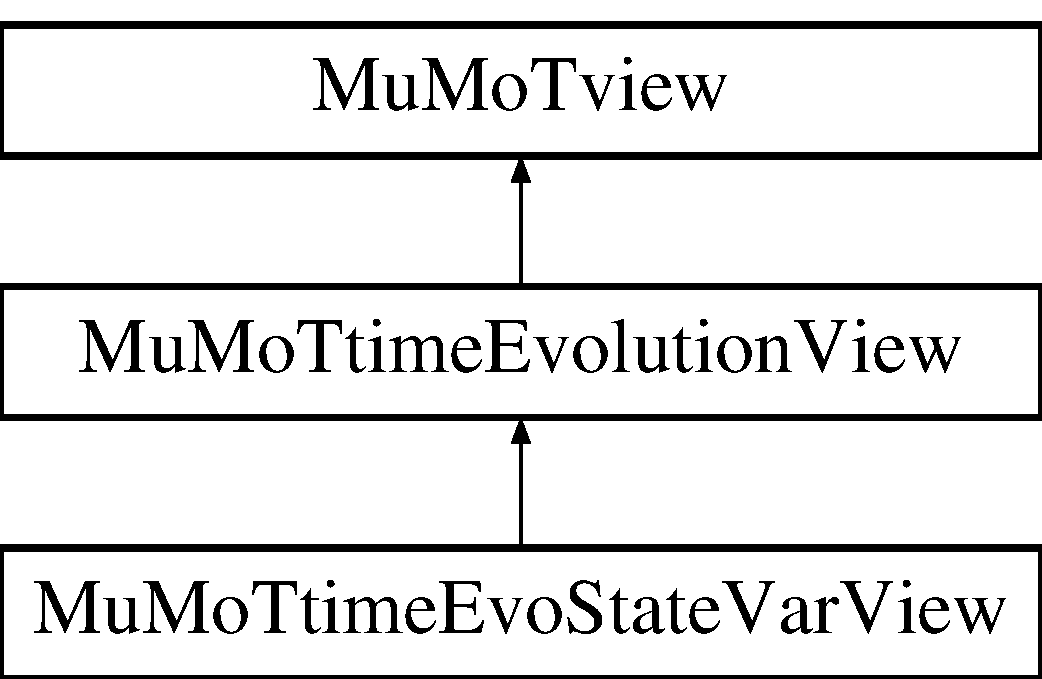
\includegraphics[height=3.000000cm]{class_mu_mo_t_1_1_mu_mo_t_1_1_mu_mo_ttime_evolution_view}
\end{center}
\end{figure}
\subsection*{Public Member Functions}
\begin{DoxyCompactItemize}
\item 
def \hyperlink{class_mu_mo_t_1_1_mu_mo_t_1_1_mu_mo_ttime_evolution_view_a5e770e35882c7ca31a269958f19a6850}{\+\_\+\+\_\+init\+\_\+\+\_\+} (self, model, controller, state\+Variable1, state\+Variable2, state\+Variable3=None, state\+Variable4=None, tend=100, tstep=0.\+01, figure=None, params=None, kwargs)
\end{DoxyCompactItemize}
\subsection*{Private Member Functions}
\begin{DoxyCompactItemize}
\item 
def \hyperlink{class_mu_mo_t_1_1_mu_mo_t_1_1_mu_mo_ttime_evolution_view_ae0c30bb947416bd557c983fe668513a8}{\+\_\+get\+Init\+Conds\+From\+Slider} (self)
\item 
def \hyperlink{class_mu_mo_t_1_1_mu_mo_t_1_1_mu_mo_ttime_evolution_view_ac73bb501e7bfd03ba030d3ec04688232}{\+\_\+get\+\_\+eqs\+O\+DE} (self, y\+\_\+old, time)
\begin{DoxyCompactList}\small\item\em calculates right-\/hand side of O\+DE system \end{DoxyCompactList}\item 
def \hyperlink{class_mu_mo_t_1_1_mu_mo_t_1_1_mu_mo_ttime_evolution_view_a588142f52d59a2abf3229d40beffbe7e}{\+\_\+plot\+\_\+\+Num\+Sol\+O\+DE} (self)
\begin{DoxyCompactList}\small\item\em calculates stationary states of 2d system def \+\_\+get\+\_\+fixed\+Points2d(self)\+: \#plot\+Limits = self.\+\_\+controller.\+\_\+get\+Plot\+Limits() param\+Names = \mbox{[}\mbox{]} param\+Values = \mbox{[}\mbox{]} if self.\+\_\+controller is not None\+: for name, value in self.\+\_\+controller.\+\_\+widgets\+Free\+Params.\+items()\+: \subsection*{throw away formatting for constant reactants}

\subsection*{name = name.\+replace(\textquotesingle{}(\textquotesingle{},\textquotesingle{}\textquotesingle{})}

\subsection*{name = name.\+replace(\textquotesingle{})\textquotesingle{},\textquotesingle{}\textquotesingle{})}

param\+Names.\+append(name) param\+Values.\+append(value.\+value) if self.\+\_\+param\+Names is not None\+: param\+Names += map(str, self.\+\_\+param\+Names) param\+Values += self.\+\_\+param\+Values funcs = self.\+\_\+mumot\+Model.\+\_\+get\+Funcs() arg\+Names\+Symb = list(map(\+Symbol, param\+Names)) arg\+Dict = dict(zip(arg\+Names\+Symb, param\+Values)) arg\+Dict\mbox{[}self.\+\_\+mumot\+Model.\+\_\+system\+Size\mbox{]} = 1 \end{DoxyCompactList}\end{DoxyCompactItemize}
\subsection*{Private Attributes}
\begin{DoxyCompactItemize}
\item 
\hyperlink{class_mu_mo_t_1_1_mu_mo_t_1_1_mu_mo_ttime_evolution_view_a6a353a1ef9443ae375948d592ed6cec6}{\+\_\+choose\+Font\+Size}
\item 
\hyperlink{class_mu_mo_t_1_1_mu_mo_t_1_1_mu_mo_ttime_evolution_view_a865b2109ba10d874e84d4a354873b121}{\+\_\+xlab}
\item 
\hyperlink{class_mu_mo_t_1_1_mu_mo_t_1_1_mu_mo_ttime_evolution_view_aac1a25a634d53e524573f67eb5f3a7b9}{\+\_\+ylab}
\item 
\hyperlink{class_mu_mo_t_1_1_mu_mo_t_1_1_mu_mo_ttime_evolution_view_a11488f79e0409b71b0bb257c81ae4687}{\+\_\+legend\+\_\+loc}
\end{DoxyCompactItemize}
\subsection*{Static Private Attributes}
\begin{DoxyCompactItemize}
\item 
\hyperlink{class_mu_mo_t_1_1_mu_mo_t_1_1_mu_mo_ttime_evolution_view_aa14fa36730691becc6f3136899545416}{\+\_\+state\+Variable1} = None
\begin{DoxyCompactList}\small\item\em 1st state variable \end{DoxyCompactList}\item 
\hyperlink{class_mu_mo_t_1_1_mu_mo_t_1_1_mu_mo_ttime_evolution_view_a9d3705d1d9182e10751ff693573d6d16}{\+\_\+state\+Variable2} = None
\begin{DoxyCompactList}\small\item\em 2nd state variable \end{DoxyCompactList}\item 
\hyperlink{class_mu_mo_t_1_1_mu_mo_t_1_1_mu_mo_ttime_evolution_view_ad2f8dc44173a16468bd9d3ab335f9b27}{\+\_\+state\+Variable3} = None
\begin{DoxyCompactList}\small\item\em 3rd state variable \end{DoxyCompactList}\item 
\hyperlink{class_mu_mo_t_1_1_mu_mo_t_1_1_mu_mo_ttime_evolution_view_a058e698cd8f7e6b6f6decd99046629a3}{\+\_\+state\+Variable4} = None
\begin{DoxyCompactList}\small\item\em 4th state variable \end{DoxyCompactList}\item 
\hyperlink{class_mu_mo_t_1_1_mu_mo_t_1_1_mu_mo_ttime_evolution_view_a27ad71f8ed3d77fd75946e5b092a228e}{\+\_\+tend} = None
\begin{DoxyCompactList}\small\item\em end time of numerical simulation \end{DoxyCompactList}\item 
\hyperlink{class_mu_mo_t_1_1_mu_mo_t_1_1_mu_mo_ttime_evolution_view_a944ca51d66346a527aa4c8938ccfbfec}{\+\_\+tstep} = None
\begin{DoxyCompactList}\small\item\em time step of numerical simulation \end{DoxyCompactList}\end{DoxyCompactItemize}
\subsection*{Additional Inherited Members}


\subsection{Detailed Description}
time evolution view on model including state variables and noise (specialised by \hyperlink{class_mu_mo_t_1_1_mu_mo_t_1_1_mu_mo_ttime_evo_state_var_view}{Mu\+Mo\+Ttime\+Evo\+State\+Var\+View} and Mu\+Mo\+Ttime\+Evo\+Noise\+View) 

\subsection{Constructor \& Destructor Documentation}
\mbox{\Hypertarget{class_mu_mo_t_1_1_mu_mo_t_1_1_mu_mo_ttime_evolution_view_a5e770e35882c7ca31a269958f19a6850}\label{class_mu_mo_t_1_1_mu_mo_t_1_1_mu_mo_ttime_evolution_view_a5e770e35882c7ca31a269958f19a6850}} 
\index{Mu\+Mo\+T\+::\+Mu\+Mo\+T\+::\+Mu\+Mo\+Ttime\+Evolution\+View@{Mu\+Mo\+T\+::\+Mu\+Mo\+T\+::\+Mu\+Mo\+Ttime\+Evolution\+View}!\+\_\+\+\_\+init\+\_\+\+\_\+@{\+\_\+\+\_\+init\+\_\+\+\_\+}}
\index{\+\_\+\+\_\+init\+\_\+\+\_\+@{\+\_\+\+\_\+init\+\_\+\+\_\+}!Mu\+Mo\+T\+::\+Mu\+Mo\+T\+::\+Mu\+Mo\+Ttime\+Evolution\+View@{Mu\+Mo\+T\+::\+Mu\+Mo\+T\+::\+Mu\+Mo\+Ttime\+Evolution\+View}}
\subsubsection{\texorpdfstring{\+\_\+\+\_\+init\+\_\+\+\_\+()}{\_\_init\_\_()}}
{\footnotesize\ttfamily def \+\_\+\+\_\+init\+\_\+\+\_\+ (\begin{DoxyParamCaption}\item[{}]{self,  }\item[{}]{model,  }\item[{}]{controller,  }\item[{}]{state\+Variable1,  }\item[{}]{state\+Variable2,  }\item[{}]{state\+Variable3 = {\ttfamily None},  }\item[{}]{state\+Variable4 = {\ttfamily None},  }\item[{}]{tend = {\ttfamily 100},  }\item[{}]{tstep = {\ttfamily 0.01},  }\item[{}]{figure = {\ttfamily None},  }\item[{}]{params = {\ttfamily None},  }\item[{}]{kwargs }\end{DoxyParamCaption})}



\subsection{Member Function Documentation}
\mbox{\Hypertarget{class_mu_mo_t_1_1_mu_mo_t_1_1_mu_mo_ttime_evolution_view_ac73bb501e7bfd03ba030d3ec04688232}\label{class_mu_mo_t_1_1_mu_mo_t_1_1_mu_mo_ttime_evolution_view_ac73bb501e7bfd03ba030d3ec04688232}} 
\index{Mu\+Mo\+T\+::\+Mu\+Mo\+T\+::\+Mu\+Mo\+Ttime\+Evolution\+View@{Mu\+Mo\+T\+::\+Mu\+Mo\+T\+::\+Mu\+Mo\+Ttime\+Evolution\+View}!\+\_\+get\+\_\+eqs\+O\+DE@{\+\_\+get\+\_\+eqs\+O\+DE}}
\index{\+\_\+get\+\_\+eqs\+O\+DE@{\+\_\+get\+\_\+eqs\+O\+DE}!Mu\+Mo\+T\+::\+Mu\+Mo\+T\+::\+Mu\+Mo\+Ttime\+Evolution\+View@{Mu\+Mo\+T\+::\+Mu\+Mo\+T\+::\+Mu\+Mo\+Ttime\+Evolution\+View}}
\subsubsection{\texorpdfstring{\+\_\+get\+\_\+eqs\+O\+D\+E()}{\_get\_eqsODE()}}
{\footnotesize\ttfamily def \+\_\+get\+\_\+eqs\+O\+DE (\begin{DoxyParamCaption}\item[{}]{self,  }\item[{}]{y\+\_\+old,  }\item[{}]{time }\end{DoxyParamCaption})\hspace{0.3cm}{\ttfamily [private]}}



calculates right-\/hand side of O\+DE system 

\mbox{\Hypertarget{class_mu_mo_t_1_1_mu_mo_t_1_1_mu_mo_ttime_evolution_view_ae0c30bb947416bd557c983fe668513a8}\label{class_mu_mo_t_1_1_mu_mo_t_1_1_mu_mo_ttime_evolution_view_ae0c30bb947416bd557c983fe668513a8}} 
\index{Mu\+Mo\+T\+::\+Mu\+Mo\+T\+::\+Mu\+Mo\+Ttime\+Evolution\+View@{Mu\+Mo\+T\+::\+Mu\+Mo\+T\+::\+Mu\+Mo\+Ttime\+Evolution\+View}!\+\_\+get\+Init\+Conds\+From\+Slider@{\+\_\+get\+Init\+Conds\+From\+Slider}}
\index{\+\_\+get\+Init\+Conds\+From\+Slider@{\+\_\+get\+Init\+Conds\+From\+Slider}!Mu\+Mo\+T\+::\+Mu\+Mo\+T\+::\+Mu\+Mo\+Ttime\+Evolution\+View@{Mu\+Mo\+T\+::\+Mu\+Mo\+T\+::\+Mu\+Mo\+Ttime\+Evolution\+View}}
\subsubsection{\texorpdfstring{\+\_\+get\+Init\+Conds\+From\+Slider()}{\_getInitCondsFromSlider()}}
{\footnotesize\ttfamily def \+\_\+get\+Init\+Conds\+From\+Slider (\begin{DoxyParamCaption}\item[{}]{self }\end{DoxyParamCaption})\hspace{0.3cm}{\ttfamily [private]}}

\mbox{\Hypertarget{class_mu_mo_t_1_1_mu_mo_t_1_1_mu_mo_ttime_evolution_view_a588142f52d59a2abf3229d40beffbe7e}\label{class_mu_mo_t_1_1_mu_mo_t_1_1_mu_mo_ttime_evolution_view_a588142f52d59a2abf3229d40beffbe7e}} 
\index{Mu\+Mo\+T\+::\+Mu\+Mo\+T\+::\+Mu\+Mo\+Ttime\+Evolution\+View@{Mu\+Mo\+T\+::\+Mu\+Mo\+T\+::\+Mu\+Mo\+Ttime\+Evolution\+View}!\+\_\+plot\+\_\+\+Num\+Sol\+O\+DE@{\+\_\+plot\+\_\+\+Num\+Sol\+O\+DE}}
\index{\+\_\+plot\+\_\+\+Num\+Sol\+O\+DE@{\+\_\+plot\+\_\+\+Num\+Sol\+O\+DE}!Mu\+Mo\+T\+::\+Mu\+Mo\+T\+::\+Mu\+Mo\+Ttime\+Evolution\+View@{Mu\+Mo\+T\+::\+Mu\+Mo\+T\+::\+Mu\+Mo\+Ttime\+Evolution\+View}}
\subsubsection{\texorpdfstring{\+\_\+plot\+\_\+\+Num\+Sol\+O\+D\+E()}{\_plot\_NumSolODE()}}
{\footnotesize\ttfamily def \+\_\+plot\+\_\+\+Num\+Sol\+O\+DE (\begin{DoxyParamCaption}\item[{}]{self }\end{DoxyParamCaption})\hspace{0.3cm}{\ttfamily [private]}}



calculates stationary states of 2d system def \+\_\+get\+\_\+fixed\+Points2d(self)\+: \#plot\+Limits = self.\+\_\+controller.\+\_\+get\+Plot\+Limits() param\+Names = \mbox{[}\mbox{]} param\+Values = \mbox{[}\mbox{]} if self.\+\_\+controller is not None\+: for name, value in self.\+\_\+controller.\+\_\+widgets\+Free\+Params.\+items()\+: \subsection*{throw away formatting for constant reactants}

\subsection*{name = name.\+replace(\textquotesingle{}(\textquotesingle{},\textquotesingle{}\textquotesingle{})}

\subsection*{name = name.\+replace(\textquotesingle{})\textquotesingle{},\textquotesingle{}\textquotesingle{})}

param\+Names.\+append(name) param\+Values.\+append(value.\+value) if self.\+\_\+param\+Names is not None\+: param\+Names += map(str, self.\+\_\+param\+Names) param\+Values += self.\+\_\+param\+Values funcs = self.\+\_\+mumot\+Model.\+\_\+get\+Funcs() arg\+Names\+Symb = list(map(\+Symbol, param\+Names)) arg\+Dict = dict(zip(arg\+Names\+Symb, param\+Values)) arg\+Dict\mbox{[}self.\+\_\+mumot\+Model.\+\_\+system\+Size\mbox{]} = 1 

E\+Q1 = self.\+\_\+mumot\+Model.\+\_\+equations\mbox{[}self.\+\_\+state\+Variable1\mbox{]}.subs(arg\+Dict) E\+Q2 = self.\+\_\+mumot\+Model.\+\_\+equations\mbox{[}self.\+\_\+state\+Variable2\mbox{]}.subs(arg\+Dict) eps=1e-\/8 E\+Qsol = solve((E\+Q1, E\+Q2), (self.\+\_\+state\+Variable1, self.\+\_\+state\+Variable2), dict=True) real\+E\+Qsol = \mbox{[}\{self.\+\_\+state\+Variable1\+: re(E\+Qsol\mbox{[}kk\mbox{]}\mbox{[}self.\+\_\+state\+Variable1\mbox{]}), self.\+\_\+state\+Variable2\+: re(E\+Qsol\mbox{[}kk\mbox{]}\mbox{[}self.\+\_\+state\+Variable2\mbox{]})\} for kk in range(len(\+E\+Qsol)) if (Abs(im(E\+Qsol\mbox{[}kk\mbox{]}\mbox{[}self.\+\_\+state\+Variable1\mbox{]}))$<$=eps and Abs(im(E\+Qsol\mbox{[}kk\mbox{]}\mbox{[}self.\+\_\+state\+Variable2\mbox{]}))$<$=eps)\mbox{]}

M\+AT = Matrix(\mbox{[}\+E\+Q1, E\+Q2\mbox{]}) J\+AC = M\+A\+T.\+jacobian(\mbox{[}self.\+\_\+state\+Variable1,self.\+\_\+state\+Variable2\mbox{]})

eig\+List = \mbox{[}\mbox{]} for nn in range(len(real\+E\+Qsol))\+: ev\+Set = \{\} J\+A\+Csub=J\+A\+C.\+subs(\mbox{[}(self.\+\_\+state\+Variable1, real\+E\+Qsol\mbox{[}nn\mbox{]}\mbox{[}self.\+\_\+state\+Variable1\mbox{]}), (self.\+\_\+state\+Variable2, real\+E\+Qsol\mbox{[}nn\mbox{]}\mbox{[}self.\+\_\+state\+Variable2\mbox{]})\mbox{]}) \#ev\+Set = J\+A\+Csub.\+eigenvals() eig\+Vects = J\+A\+Csub.\+eigenvects() for kk in range(len(eig\+Vects))\+: ev\+Set\mbox{[}eig\+Vects\mbox{[}kk\mbox{]}\mbox{[}0\mbox{]}\mbox{]} = (eig\+Vects\mbox{[}kk\mbox{]}\mbox{[}1\mbox{]}, eig\+Vects\mbox{[}kk\mbox{]}\mbox{[}2\mbox{]}) eig\+List.\+append(ev\+Set) return real\+E\+Qsol, eig\+List \#returns two lists of dictionaries

\subsubsection*{calculates stationary states of 3d system}

def \+\_\+get\+\_\+fixed\+Points3d(self)\+: \#plot\+Limits = self.\+\_\+controller.\+\_\+get\+Plot\+Limits() param\+Names = \mbox{[}\mbox{]} param\+Values = \mbox{[}\mbox{]} if self.\+\_\+controller != None\+: for name, value in self.\+\_\+controller.\+\_\+widgets\+Free\+Params.\+items()\+: \subsection*{throw away formatting for constant reactants}

\subsection*{name = name.\+replace(\textquotesingle{}(\textquotesingle{},\textquotesingle{}\textquotesingle{})}

\subsection*{name = name.\+replace(\textquotesingle{})\textquotesingle{},\textquotesingle{}\textquotesingle{})}

param\+Names.\+append(name) param\+Values.\+append(value.\+value) if self.\+\_\+param\+Names is not None\+: param\+Names += map(str, self.\+\_\+param\+Names) param\+Values += self.\+\_\+param\+Values funcs = self.\+\_\+mumot\+Model.\+\_\+get\+Funcs() arg\+Names\+Symb = list(map(\+Symbol, param\+Names)) arg\+Dict = dict(zip(arg\+Names\+Symb, param\+Values)) arg\+Dict\mbox{[}self.\+\_\+mumot\+Model.\+\_\+system\+Size\mbox{]} = 1

E\+Q1 = self.\+\_\+mumot\+Model.\+\_\+equations\mbox{[}self.\+\_\+state\+Variable1\mbox{]}.subs(arg\+Dict) E\+Q2 = self.\+\_\+mumot\+Model.\+\_\+equations\mbox{[}self.\+\_\+state\+Variable2\mbox{]}.subs(arg\+Dict) E\+Q3 = self.\+\_\+mumot\+Model.\+\_\+equations\mbox{[}self.\+\_\+state\+Variable3\mbox{]}.subs(arg\+Dict) eps=1e-\/8 E\+Qsol = solve((E\+Q1, E\+Q2, E\+Q3), (self.\+\_\+state\+Variable1, self.\+\_\+state\+Variable2, self.\+\_\+state\+Variable3), dict=True) real\+E\+Qsol = \mbox{[}\{self.\+\_\+state\+Variable1\+: re(E\+Qsol\mbox{[}kk\mbox{]}\mbox{[}self.\+\_\+state\+Variable1\mbox{]}), self.\+\_\+state\+Variable2\+: re(E\+Qsol\mbox{[}kk\mbox{]}\mbox{[}self.\+\_\+state\+Variable2\mbox{]}), self.\+\_\+state\+Variable3\+: re(E\+Qsol\mbox{[}kk\mbox{]}\mbox{[}self.\+\_\+state\+Variable3\mbox{]})\} for kk in range(len(\+E\+Qsol)) if (Abs(im(E\+Qsol\mbox{[}kk\mbox{]}\mbox{[}self.\+\_\+state\+Variable1\mbox{]}))$<$=eps and Abs(im(E\+Qsol\mbox{[}kk\mbox{]}\mbox{[}self.\+\_\+state\+Variable2\mbox{]}))$<$=eps and Abs(im(E\+Qsol\mbox{[}kk\mbox{]}\mbox{[}self.\+\_\+state\+Variable3\mbox{]}))$<$=eps)\mbox{]}

M\+AT = Matrix(\mbox{[}\+E\+Q1, E\+Q2, E\+Q3\mbox{]}) J\+AC = M\+A\+T.\+jacobian(\mbox{[}self.\+\_\+state\+Variable1,self.\+\_\+state\+Variable2,self.\+\_\+state\+Variable3\mbox{]})

eig\+List = \mbox{[}\mbox{]} for nn in range(len(real\+E\+Qsol))\+: ev\+Set = \{\} J\+A\+Csub=J\+A\+C.\+subs(\mbox{[}(self.\+\_\+state\+Variable1, real\+E\+Qsol\mbox{[}nn\mbox{]}\mbox{[}self.\+\_\+state\+Variable1\mbox{]}), (self.\+\_\+state\+Variable2, real\+E\+Qsol\mbox{[}nn\mbox{]}\mbox{[}self.\+\_\+state\+Variable2\mbox{]}), (self.\+\_\+state\+Variable3, real\+E\+Qsol\mbox{[}nn\mbox{]}\mbox{[}self.\+\_\+state\+Variable3\mbox{]})\mbox{]}) \#ev\+Set = J\+A\+Csub.\+eigenvals() eig\+Vects = J\+A\+Csub.\+eigenvects() for kk in range(len(eig\+Vects))\+: ev\+Set\mbox{[}eig\+Vects\mbox{[}kk\mbox{]}\mbox{[}0\mbox{]}\mbox{]} = (eig\+Vects\mbox{[}kk\mbox{]}\mbox{[}1\mbox{]}, eig\+Vects\mbox{[}kk\mbox{]}\mbox{[}2\mbox{]}) eig\+List.\+append(ev\+Set) return real\+E\+Qsol, eig\+List \#returns two lists of dictionaries 

\subsection{Field Documentation}
\mbox{\Hypertarget{class_mu_mo_t_1_1_mu_mo_t_1_1_mu_mo_ttime_evolution_view_a6a353a1ef9443ae375948d592ed6cec6}\label{class_mu_mo_t_1_1_mu_mo_t_1_1_mu_mo_ttime_evolution_view_a6a353a1ef9443ae375948d592ed6cec6}} 
\index{Mu\+Mo\+T\+::\+Mu\+Mo\+T\+::\+Mu\+Mo\+Ttime\+Evolution\+View@{Mu\+Mo\+T\+::\+Mu\+Mo\+T\+::\+Mu\+Mo\+Ttime\+Evolution\+View}!\+\_\+choose\+Font\+Size@{\+\_\+choose\+Font\+Size}}
\index{\+\_\+choose\+Font\+Size@{\+\_\+choose\+Font\+Size}!Mu\+Mo\+T\+::\+Mu\+Mo\+T\+::\+Mu\+Mo\+Ttime\+Evolution\+View@{Mu\+Mo\+T\+::\+Mu\+Mo\+T\+::\+Mu\+Mo\+Ttime\+Evolution\+View}}
\subsubsection{\texorpdfstring{\+\_\+choose\+Font\+Size}{\_chooseFontSize}}
{\footnotesize\ttfamily \+\_\+choose\+Font\+Size\hspace{0.3cm}{\ttfamily [private]}}

\mbox{\Hypertarget{class_mu_mo_t_1_1_mu_mo_t_1_1_mu_mo_ttime_evolution_view_a11488f79e0409b71b0bb257c81ae4687}\label{class_mu_mo_t_1_1_mu_mo_t_1_1_mu_mo_ttime_evolution_view_a11488f79e0409b71b0bb257c81ae4687}} 
\index{Mu\+Mo\+T\+::\+Mu\+Mo\+T\+::\+Mu\+Mo\+Ttime\+Evolution\+View@{Mu\+Mo\+T\+::\+Mu\+Mo\+T\+::\+Mu\+Mo\+Ttime\+Evolution\+View}!\+\_\+legend\+\_\+loc@{\+\_\+legend\+\_\+loc}}
\index{\+\_\+legend\+\_\+loc@{\+\_\+legend\+\_\+loc}!Mu\+Mo\+T\+::\+Mu\+Mo\+T\+::\+Mu\+Mo\+Ttime\+Evolution\+View@{Mu\+Mo\+T\+::\+Mu\+Mo\+T\+::\+Mu\+Mo\+Ttime\+Evolution\+View}}
\subsubsection{\texorpdfstring{\+\_\+legend\+\_\+loc}{\_legend\_loc}}
{\footnotesize\ttfamily \+\_\+legend\+\_\+loc\hspace{0.3cm}{\ttfamily [private]}}

\mbox{\Hypertarget{class_mu_mo_t_1_1_mu_mo_t_1_1_mu_mo_ttime_evolution_view_aa14fa36730691becc6f3136899545416}\label{class_mu_mo_t_1_1_mu_mo_t_1_1_mu_mo_ttime_evolution_view_aa14fa36730691becc6f3136899545416}} 
\index{Mu\+Mo\+T\+::\+Mu\+Mo\+T\+::\+Mu\+Mo\+Ttime\+Evolution\+View@{Mu\+Mo\+T\+::\+Mu\+Mo\+T\+::\+Mu\+Mo\+Ttime\+Evolution\+View}!\+\_\+state\+Variable1@{\+\_\+state\+Variable1}}
\index{\+\_\+state\+Variable1@{\+\_\+state\+Variable1}!Mu\+Mo\+T\+::\+Mu\+Mo\+T\+::\+Mu\+Mo\+Ttime\+Evolution\+View@{Mu\+Mo\+T\+::\+Mu\+Mo\+T\+::\+Mu\+Mo\+Ttime\+Evolution\+View}}
\subsubsection{\texorpdfstring{\+\_\+state\+Variable1}{\_stateVariable1}}
{\footnotesize\ttfamily \+\_\+state\+Variable1 = None\hspace{0.3cm}{\ttfamily [static]}, {\ttfamily [private]}}



1st state variable 

\mbox{\Hypertarget{class_mu_mo_t_1_1_mu_mo_t_1_1_mu_mo_ttime_evolution_view_a9d3705d1d9182e10751ff693573d6d16}\label{class_mu_mo_t_1_1_mu_mo_t_1_1_mu_mo_ttime_evolution_view_a9d3705d1d9182e10751ff693573d6d16}} 
\index{Mu\+Mo\+T\+::\+Mu\+Mo\+T\+::\+Mu\+Mo\+Ttime\+Evolution\+View@{Mu\+Mo\+T\+::\+Mu\+Mo\+T\+::\+Mu\+Mo\+Ttime\+Evolution\+View}!\+\_\+state\+Variable2@{\+\_\+state\+Variable2}}
\index{\+\_\+state\+Variable2@{\+\_\+state\+Variable2}!Mu\+Mo\+T\+::\+Mu\+Mo\+T\+::\+Mu\+Mo\+Ttime\+Evolution\+View@{Mu\+Mo\+T\+::\+Mu\+Mo\+T\+::\+Mu\+Mo\+Ttime\+Evolution\+View}}
\subsubsection{\texorpdfstring{\+\_\+state\+Variable2}{\_stateVariable2}}
{\footnotesize\ttfamily \+\_\+state\+Variable2 = None\hspace{0.3cm}{\ttfamily [static]}, {\ttfamily [private]}}



2nd state variable 

\mbox{\Hypertarget{class_mu_mo_t_1_1_mu_mo_t_1_1_mu_mo_ttime_evolution_view_ad2f8dc44173a16468bd9d3ab335f9b27}\label{class_mu_mo_t_1_1_mu_mo_t_1_1_mu_mo_ttime_evolution_view_ad2f8dc44173a16468bd9d3ab335f9b27}} 
\index{Mu\+Mo\+T\+::\+Mu\+Mo\+T\+::\+Mu\+Mo\+Ttime\+Evolution\+View@{Mu\+Mo\+T\+::\+Mu\+Mo\+T\+::\+Mu\+Mo\+Ttime\+Evolution\+View}!\+\_\+state\+Variable3@{\+\_\+state\+Variable3}}
\index{\+\_\+state\+Variable3@{\+\_\+state\+Variable3}!Mu\+Mo\+T\+::\+Mu\+Mo\+T\+::\+Mu\+Mo\+Ttime\+Evolution\+View@{Mu\+Mo\+T\+::\+Mu\+Mo\+T\+::\+Mu\+Mo\+Ttime\+Evolution\+View}}
\subsubsection{\texorpdfstring{\+\_\+state\+Variable3}{\_stateVariable3}}
{\footnotesize\ttfamily \+\_\+state\+Variable3 = None\hspace{0.3cm}{\ttfamily [static]}, {\ttfamily [private]}}



3rd state variable 

\mbox{\Hypertarget{class_mu_mo_t_1_1_mu_mo_t_1_1_mu_mo_ttime_evolution_view_a058e698cd8f7e6b6f6decd99046629a3}\label{class_mu_mo_t_1_1_mu_mo_t_1_1_mu_mo_ttime_evolution_view_a058e698cd8f7e6b6f6decd99046629a3}} 
\index{Mu\+Mo\+T\+::\+Mu\+Mo\+T\+::\+Mu\+Mo\+Ttime\+Evolution\+View@{Mu\+Mo\+T\+::\+Mu\+Mo\+T\+::\+Mu\+Mo\+Ttime\+Evolution\+View}!\+\_\+state\+Variable4@{\+\_\+state\+Variable4}}
\index{\+\_\+state\+Variable4@{\+\_\+state\+Variable4}!Mu\+Mo\+T\+::\+Mu\+Mo\+T\+::\+Mu\+Mo\+Ttime\+Evolution\+View@{Mu\+Mo\+T\+::\+Mu\+Mo\+T\+::\+Mu\+Mo\+Ttime\+Evolution\+View}}
\subsubsection{\texorpdfstring{\+\_\+state\+Variable4}{\_stateVariable4}}
{\footnotesize\ttfamily \+\_\+state\+Variable4 = None\hspace{0.3cm}{\ttfamily [static]}, {\ttfamily [private]}}



4th state variable 

\mbox{\Hypertarget{class_mu_mo_t_1_1_mu_mo_t_1_1_mu_mo_ttime_evolution_view_a27ad71f8ed3d77fd75946e5b092a228e}\label{class_mu_mo_t_1_1_mu_mo_t_1_1_mu_mo_ttime_evolution_view_a27ad71f8ed3d77fd75946e5b092a228e}} 
\index{Mu\+Mo\+T\+::\+Mu\+Mo\+T\+::\+Mu\+Mo\+Ttime\+Evolution\+View@{Mu\+Mo\+T\+::\+Mu\+Mo\+T\+::\+Mu\+Mo\+Ttime\+Evolution\+View}!\+\_\+tend@{\+\_\+tend}}
\index{\+\_\+tend@{\+\_\+tend}!Mu\+Mo\+T\+::\+Mu\+Mo\+T\+::\+Mu\+Mo\+Ttime\+Evolution\+View@{Mu\+Mo\+T\+::\+Mu\+Mo\+T\+::\+Mu\+Mo\+Ttime\+Evolution\+View}}
\subsubsection{\texorpdfstring{\+\_\+tend}{\_tend}}
{\footnotesize\ttfamily \+\_\+tend = None\hspace{0.3cm}{\ttfamily [static]}, {\ttfamily [private]}}



end time of numerical simulation 

\mbox{\Hypertarget{class_mu_mo_t_1_1_mu_mo_t_1_1_mu_mo_ttime_evolution_view_a944ca51d66346a527aa4c8938ccfbfec}\label{class_mu_mo_t_1_1_mu_mo_t_1_1_mu_mo_ttime_evolution_view_a944ca51d66346a527aa4c8938ccfbfec}} 
\index{Mu\+Mo\+T\+::\+Mu\+Mo\+T\+::\+Mu\+Mo\+Ttime\+Evolution\+View@{Mu\+Mo\+T\+::\+Mu\+Mo\+T\+::\+Mu\+Mo\+Ttime\+Evolution\+View}!\+\_\+tstep@{\+\_\+tstep}}
\index{\+\_\+tstep@{\+\_\+tstep}!Mu\+Mo\+T\+::\+Mu\+Mo\+T\+::\+Mu\+Mo\+Ttime\+Evolution\+View@{Mu\+Mo\+T\+::\+Mu\+Mo\+T\+::\+Mu\+Mo\+Ttime\+Evolution\+View}}
\subsubsection{\texorpdfstring{\+\_\+tstep}{\_tstep}}
{\footnotesize\ttfamily \+\_\+tstep = None\hspace{0.3cm}{\ttfamily [static]}, {\ttfamily [private]}}



time step of numerical simulation 

\mbox{\Hypertarget{class_mu_mo_t_1_1_mu_mo_t_1_1_mu_mo_ttime_evolution_view_a865b2109ba10d874e84d4a354873b121}\label{class_mu_mo_t_1_1_mu_mo_t_1_1_mu_mo_ttime_evolution_view_a865b2109ba10d874e84d4a354873b121}} 
\index{Mu\+Mo\+T\+::\+Mu\+Mo\+T\+::\+Mu\+Mo\+Ttime\+Evolution\+View@{Mu\+Mo\+T\+::\+Mu\+Mo\+T\+::\+Mu\+Mo\+Ttime\+Evolution\+View}!\+\_\+xlab@{\+\_\+xlab}}
\index{\+\_\+xlab@{\+\_\+xlab}!Mu\+Mo\+T\+::\+Mu\+Mo\+T\+::\+Mu\+Mo\+Ttime\+Evolution\+View@{Mu\+Mo\+T\+::\+Mu\+Mo\+T\+::\+Mu\+Mo\+Ttime\+Evolution\+View}}
\subsubsection{\texorpdfstring{\+\_\+xlab}{\_xlab}}
{\footnotesize\ttfamily \+\_\+xlab\hspace{0.3cm}{\ttfamily [private]}}

\mbox{\Hypertarget{class_mu_mo_t_1_1_mu_mo_t_1_1_mu_mo_ttime_evolution_view_aac1a25a634d53e524573f67eb5f3a7b9}\label{class_mu_mo_t_1_1_mu_mo_t_1_1_mu_mo_ttime_evolution_view_aac1a25a634d53e524573f67eb5f3a7b9}} 
\index{Mu\+Mo\+T\+::\+Mu\+Mo\+T\+::\+Mu\+Mo\+Ttime\+Evolution\+View@{Mu\+Mo\+T\+::\+Mu\+Mo\+T\+::\+Mu\+Mo\+Ttime\+Evolution\+View}!\+\_\+ylab@{\+\_\+ylab}}
\index{\+\_\+ylab@{\+\_\+ylab}!Mu\+Mo\+T\+::\+Mu\+Mo\+T\+::\+Mu\+Mo\+Ttime\+Evolution\+View@{Mu\+Mo\+T\+::\+Mu\+Mo\+T\+::\+Mu\+Mo\+Ttime\+Evolution\+View}}
\subsubsection{\texorpdfstring{\+\_\+ylab}{\_ylab}}
{\footnotesize\ttfamily \+\_\+ylab\hspace{0.3cm}{\ttfamily [private]}}



The documentation for this class was generated from the following file\+:\begin{DoxyCompactItemize}
\item 
Mu\+Mo\+T/\hyperlink{_mu_mo_t_8py}{Mu\+Mo\+T.\+py}\end{DoxyCompactItemize}

\hypertarget{class_mu_mo_t_1_1_mu_mo_t_1_1_mu_mo_ttime_evo_state_var_view}{}\section{Mu\+Mo\+Ttime\+Evo\+State\+Var\+View Class Reference}
\label{class_mu_mo_t_1_1_mu_mo_t_1_1_mu_mo_ttime_evo_state_var_view}\index{Mu\+Mo\+Ttime\+Evo\+State\+Var\+View@{Mu\+Mo\+Ttime\+Evo\+State\+Var\+View}}


numerical solution of state variables plot view on model  


Inheritance diagram for Mu\+Mo\+Ttime\+Evo\+State\+Var\+View\+:\begin{figure}[H]
\begin{center}
\leavevmode
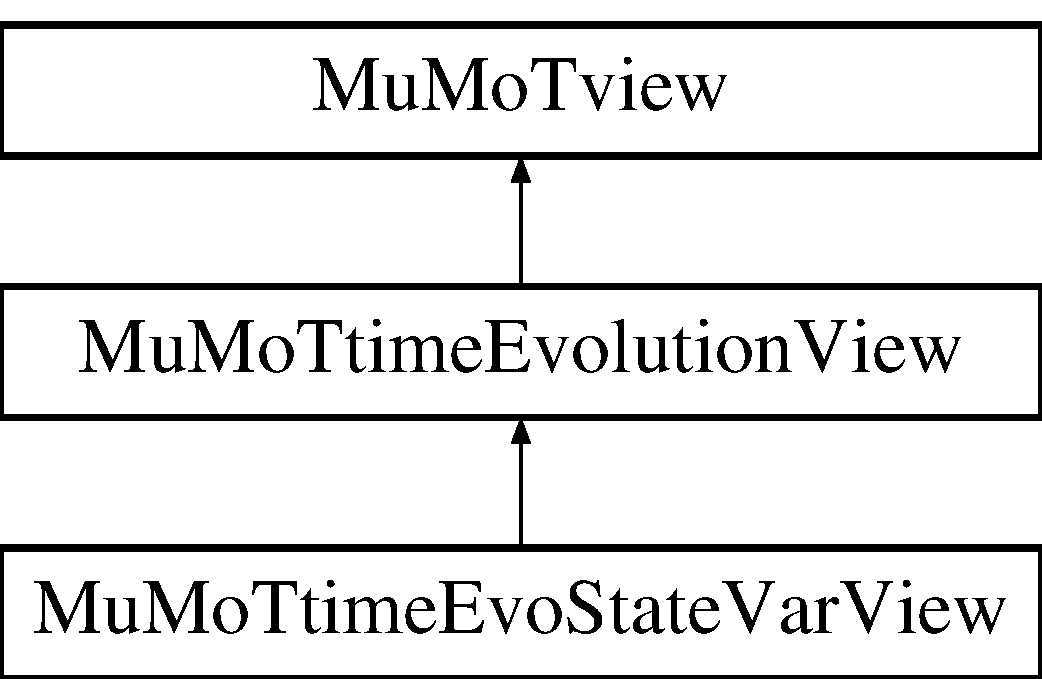
\includegraphics[height=3.000000cm]{class_mu_mo_t_1_1_mu_mo_t_1_1_mu_mo_ttime_evo_state_var_view}
\end{center}
\end{figure}
\subsection*{Public Member Functions}
\begin{DoxyCompactItemize}
\item 
def \hyperlink{class_mu_mo_t_1_1_mu_mo_t_1_1_mu_mo_ttime_evo_state_var_view_a302afe6819b093163cc8ea6f029c75da}{\+\_\+\+\_\+init\+\_\+\+\_\+} (self, args, kwargs)
\end{DoxyCompactItemize}
\subsection*{Private Member Functions}
\begin{DoxyCompactItemize}
\item 
def \hyperlink{class_mu_mo_t_1_1_mu_mo_t_1_1_mu_mo_ttime_evo_state_var_view_a588142f52d59a2abf3229d40beffbe7e}{\+\_\+plot\+\_\+\+Num\+Sol\+O\+DE} (self)
\end{DoxyCompactItemize}
\subsection*{Private Attributes}
\begin{DoxyCompactItemize}
\item 
\hyperlink{class_mu_mo_t_1_1_mu_mo_t_1_1_mu_mo_ttime_evo_state_var_view_ace48ed03490093d8f44cde91e2f1e86e}{\+\_\+generating\+Command}
\end{DoxyCompactItemize}
\subsection*{Additional Inherited Members}


\subsection{Detailed Description}
numerical solution of state variables plot view on model 

\subsection{Constructor \& Destructor Documentation}
\mbox{\Hypertarget{class_mu_mo_t_1_1_mu_mo_t_1_1_mu_mo_ttime_evo_state_var_view_a302afe6819b093163cc8ea6f029c75da}\label{class_mu_mo_t_1_1_mu_mo_t_1_1_mu_mo_ttime_evo_state_var_view_a302afe6819b093163cc8ea6f029c75da}} 
\index{Mu\+Mo\+T\+::\+Mu\+Mo\+T\+::\+Mu\+Mo\+Ttime\+Evo\+State\+Var\+View@{Mu\+Mo\+T\+::\+Mu\+Mo\+T\+::\+Mu\+Mo\+Ttime\+Evo\+State\+Var\+View}!\+\_\+\+\_\+init\+\_\+\+\_\+@{\+\_\+\+\_\+init\+\_\+\+\_\+}}
\index{\+\_\+\+\_\+init\+\_\+\+\_\+@{\+\_\+\+\_\+init\+\_\+\+\_\+}!Mu\+Mo\+T\+::\+Mu\+Mo\+T\+::\+Mu\+Mo\+Ttime\+Evo\+State\+Var\+View@{Mu\+Mo\+T\+::\+Mu\+Mo\+T\+::\+Mu\+Mo\+Ttime\+Evo\+State\+Var\+View}}
\subsubsection{\texorpdfstring{\+\_\+\+\_\+init\+\_\+\+\_\+()}{\_\_init\_\_()}}
{\footnotesize\ttfamily def \+\_\+\+\_\+init\+\_\+\+\_\+ (\begin{DoxyParamCaption}\item[{}]{self,  }\item[{}]{args,  }\item[{}]{kwargs }\end{DoxyParamCaption})}



\subsection{Member Function Documentation}
\mbox{\Hypertarget{class_mu_mo_t_1_1_mu_mo_t_1_1_mu_mo_ttime_evo_state_var_view_a588142f52d59a2abf3229d40beffbe7e}\label{class_mu_mo_t_1_1_mu_mo_t_1_1_mu_mo_ttime_evo_state_var_view_a588142f52d59a2abf3229d40beffbe7e}} 
\index{Mu\+Mo\+T\+::\+Mu\+Mo\+T\+::\+Mu\+Mo\+Ttime\+Evo\+State\+Var\+View@{Mu\+Mo\+T\+::\+Mu\+Mo\+T\+::\+Mu\+Mo\+Ttime\+Evo\+State\+Var\+View}!\+\_\+plot\+\_\+\+Num\+Sol\+O\+DE@{\+\_\+plot\+\_\+\+Num\+Sol\+O\+DE}}
\index{\+\_\+plot\+\_\+\+Num\+Sol\+O\+DE@{\+\_\+plot\+\_\+\+Num\+Sol\+O\+DE}!Mu\+Mo\+T\+::\+Mu\+Mo\+T\+::\+Mu\+Mo\+Ttime\+Evo\+State\+Var\+View@{Mu\+Mo\+T\+::\+Mu\+Mo\+T\+::\+Mu\+Mo\+Ttime\+Evo\+State\+Var\+View}}
\subsubsection{\texorpdfstring{\+\_\+plot\+\_\+\+Num\+Sol\+O\+D\+E()}{\_plot\_NumSolODE()}}
{\footnotesize\ttfamily def \+\_\+plot\+\_\+\+Num\+Sol\+O\+DE (\begin{DoxyParamCaption}\item[{}]{self }\end{DoxyParamCaption})\hspace{0.3cm}{\ttfamily [private]}}



\subsection{Field Documentation}
\mbox{\Hypertarget{class_mu_mo_t_1_1_mu_mo_t_1_1_mu_mo_ttime_evo_state_var_view_ace48ed03490093d8f44cde91e2f1e86e}\label{class_mu_mo_t_1_1_mu_mo_t_1_1_mu_mo_ttime_evo_state_var_view_ace48ed03490093d8f44cde91e2f1e86e}} 
\index{Mu\+Mo\+T\+::\+Mu\+Mo\+T\+::\+Mu\+Mo\+Ttime\+Evo\+State\+Var\+View@{Mu\+Mo\+T\+::\+Mu\+Mo\+T\+::\+Mu\+Mo\+Ttime\+Evo\+State\+Var\+View}!\+\_\+generating\+Command@{\+\_\+generating\+Command}}
\index{\+\_\+generating\+Command@{\+\_\+generating\+Command}!Mu\+Mo\+T\+::\+Mu\+Mo\+T\+::\+Mu\+Mo\+Ttime\+Evo\+State\+Var\+View@{Mu\+Mo\+T\+::\+Mu\+Mo\+T\+::\+Mu\+Mo\+Ttime\+Evo\+State\+Var\+View}}
\subsubsection{\texorpdfstring{\+\_\+generating\+Command}{\_generatingCommand}}
{\footnotesize\ttfamily \+\_\+generating\+Command\hspace{0.3cm}{\ttfamily [private]}}



The documentation for this class was generated from the following file\+:\begin{DoxyCompactItemize}
\item 
Mu\+Mo\+T/\hyperlink{_mu_mo_t_8py}{Mu\+Mo\+T.\+py}\end{DoxyCompactItemize}

\hypertarget{class_mu_mo_t_1_1_mu_mo_t_1_1_mu_mo_tvector_view}{}\section{Mu\+Mo\+Tvector\+View Class Reference}
\label{class_mu_mo_t_1_1_mu_mo_t_1_1_mu_mo_tvector_view}\index{Mu\+Mo\+Tvector\+View@{Mu\+Mo\+Tvector\+View}}


vector plot view on model  


Inheritance diagram for Mu\+Mo\+Tvector\+View\+:\begin{figure}[H]
\begin{center}
\leavevmode
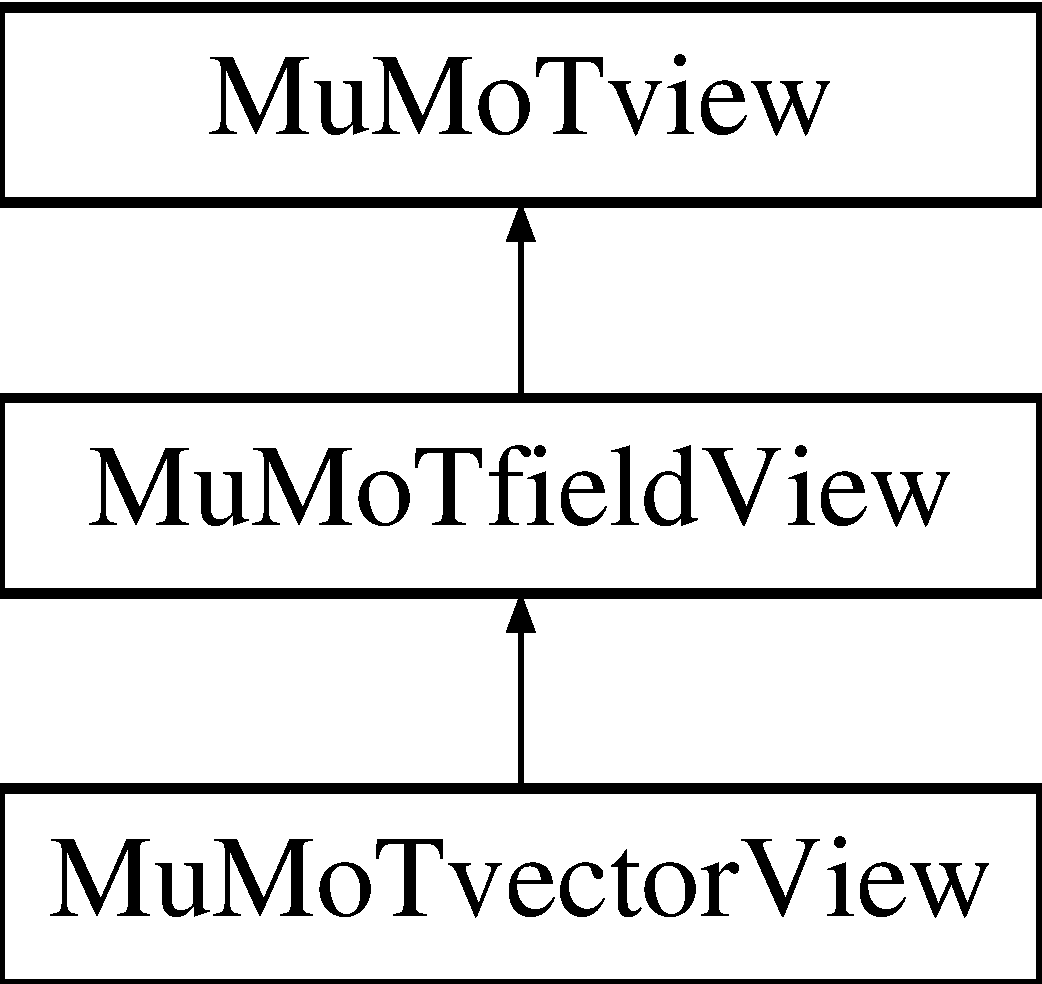
\includegraphics[height=3.000000cm]{class_mu_mo_t_1_1_mu_mo_t_1_1_mu_mo_tvector_view}
\end{center}
\end{figure}
\subsection*{Public Member Functions}
\begin{DoxyCompactItemize}
\item 
def \hyperlink{class_mu_mo_t_1_1_mu_mo_t_1_1_mu_mo_tvector_view_a302afe6819b093163cc8ea6f029c75da}{\+\_\+\+\_\+init\+\_\+\+\_\+} (self, args, kwargs)
\end{DoxyCompactItemize}
\subsection*{Static Public Attributes}
\begin{DoxyCompactItemize}
\item 
\hyperlink{class_mu_mo_t_1_1_mu_mo_t_1_1_mu_mo_tvector_view_ab964c8e9f2533c9bf4957faf67de7149}{real\+E\+Qsol}
\item 
\hyperlink{class_mu_mo_t_1_1_mu_mo_t_1_1_mu_mo_tvector_view_ab5666bb0356c5bc211c10fd59723e892}{eig\+List}
\item 
list \hyperlink{class_mu_mo_t_1_1_mu_mo_t_1_1_mu_mo_tvector_view_ab56bd718f01a64e681a8135a8e90946a}{EV} = \mbox{[}$\,$\mbox{]}
\item 
list \hyperlink{class_mu_mo_t_1_1_mu_mo_t_1_1_mu_mo_tvector_view_a424471486fdcd104bad36c06ae6c8640}{E\+Vplot} = \mbox{[}$\,$\mbox{]}
\item 
list \hyperlink{class_mu_mo_t_1_1_mu_mo_t_1_1_mu_mo_tvector_view_a5b825ad4fea91f83e5f0df2bda4278f9}{E\+Vsub} = \mbox{[}$\,$\mbox{]}
\item 
list \hyperlink{class_mu_mo_t_1_1_mu_mo_t_1_1_mu_mo_tvector_view_aac20660098bbbe33ab90f9c880b2fa8c}{Fixed\+Points}
\item 
\hyperlink{class_mu_mo_t_1_1_mu_mo_t_1_1_mu_mo_tvector_view_a7a971a839d61106558ebf0453849cfd1}{Fixed\+Points} = None
\item 
\hyperlink{class_mu_mo_t_1_1_mu_mo_t_1_1_mu_mo_tvector_view_a8fa675eb2fcec5b95d9d21c670da7f30}{ax} = self.\+\_\+figure.\+gca(projection = \textquotesingle{}3d\textquotesingle{})
\item 
\hyperlink{class_mu_mo_t_1_1_mu_mo_t_1_1_mu_mo_tvector_view_a0d21a210e4f523569e4c57a12f80040c}{fig\+\_\+vec3d} = ax.\+quiver(self.\+\_\+X, self.\+\_\+Y, self.\+\_\+Z, self.\+\_\+\+Xdot, self.\+\_\+\+Ydot, self.\+\_\+\+Zdot, length = 0.\+01, \hyperlink{class_mu_mo_t_1_1_mu_mo_t_1_1_mu_mo_tview_a37dbdc30935031c05304482e1be89d8f}{color} = \textquotesingle{}black\textquotesingle{})
\item 
\hyperlink{class_mu_mo_t_1_1_mu_mo_t_1_1_mu_mo_tvector_view_a391e34f2de441d79152a7b3d6e4c9c86}{figure}
\item 
\hyperlink{class_mu_mo_t_1_1_mu_mo_t_1_1_mu_mo_tvector_view_abb76a7390100209788848dbd6bb9fe30}{xlab}
\item 
\hyperlink{class_mu_mo_t_1_1_mu_mo_t_1_1_mu_mo_tvector_view_a83433d4e45c13afe9a0042ae113ad169}{ylab}
\item 
\hyperlink{class_mu_mo_t_1_1_mu_mo_t_1_1_mu_mo_tvector_view_a180fbd5bd60d175c88a69e1dd3b0ed77}{zlab}
\item 
\hyperlink{class_mu_mo_t_1_1_mu_mo_t_1_1_mu_mo_tvector_view_a3c1c635ffc7ed4d381b8c672ebfac0fb}{special\+Points}
\item 
\hyperlink{class_mu_mo_t_1_1_mu_mo_t_1_1_mu_mo_tvector_view_a22d867cfa21f7f37efee834159e18983}{show\+Fixed\+Points}
\item 
\hyperlink{class_mu_mo_t_1_1_mu_mo_t_1_1_mu_mo_tvector_view_a73c8f7f0d9593ed55a0cb1bea896b9f4}{ax\+\_\+reformat}
\item 
\hyperlink{class_mu_mo_t_1_1_mu_mo_t_1_1_mu_mo_tvector_view_a643a20c0c59588a0f741a6095e2025fd}{True}
\item 
\hyperlink{class_mu_mo_t_1_1_mu_mo_t_1_1_mu_mo_tvector_view_a44c38482b3d22d05f8bbadb81ec2d40a}{show\+Plane}
\end{DoxyCompactItemize}
\subsection*{Private Member Functions}
\begin{DoxyCompactItemize}
\item 
def \hyperlink{class_mu_mo_t_1_1_mu_mo_t_1_1_mu_mo_tvector_view_a50d59419298116f738a98c864afb9d89}{\+\_\+plot\+\_\+field} (self)
\end{DoxyCompactItemize}
\subsection*{Private Attributes}
\begin{DoxyCompactItemize}
\item 
\hyperlink{class_mu_mo_t_1_1_mu_mo_t_1_1_mu_mo_tvector_view_ace48ed03490093d8f44cde91e2f1e86e}{\+\_\+generating\+Command}
\item 
\hyperlink{class_mu_mo_t_1_1_mu_mo_t_1_1_mu_mo_tvector_view_ad2f8dc44173a16468bd9d3ab335f9b27}{\+\_\+state\+Variable3}
\end{DoxyCompactItemize}
\subsection*{Static Private Attributes}
\begin{DoxyCompactItemize}
\item 
\hyperlink{class_mu_mo_t_1_1_mu_mo_t_1_1_mu_mo_tvector_view_a865b2109ba10d874e84d4a354873b121}{\+\_\+xlab}
\item 
\hyperlink{class_mu_mo_t_1_1_mu_mo_t_1_1_mu_mo_tvector_view_aac1a25a634d53e524573f67eb5f3a7b9}{\+\_\+ylab}
\item 
\hyperlink{class_mu_mo_t_1_1_mu_mo_t_1_1_mu_mo_tvector_view_afcc07605f40039b605802f93b39ea910}{\+\_\+zlab}
\item 
\hyperlink{class_mu_mo_t_1_1_mu_mo_t_1_1_mu_mo_tvector_view_ac83a924ad62a2461d65b5c9bf9d27453}{\+\_\+show\+Fixed\+Points}
\end{DoxyCompactItemize}


\subsection{Detailed Description}
vector plot view on model 

\subsection{Constructor \& Destructor Documentation}
\mbox{\Hypertarget{class_mu_mo_t_1_1_mu_mo_t_1_1_mu_mo_tvector_view_a302afe6819b093163cc8ea6f029c75da}\label{class_mu_mo_t_1_1_mu_mo_t_1_1_mu_mo_tvector_view_a302afe6819b093163cc8ea6f029c75da}} 
\index{Mu\+Mo\+T\+::\+Mu\+Mo\+T\+::\+Mu\+Mo\+Tvector\+View@{Mu\+Mo\+T\+::\+Mu\+Mo\+T\+::\+Mu\+Mo\+Tvector\+View}!\+\_\+\+\_\+init\+\_\+\+\_\+@{\+\_\+\+\_\+init\+\_\+\+\_\+}}
\index{\+\_\+\+\_\+init\+\_\+\+\_\+@{\+\_\+\+\_\+init\+\_\+\+\_\+}!Mu\+Mo\+T\+::\+Mu\+Mo\+T\+::\+Mu\+Mo\+Tvector\+View@{Mu\+Mo\+T\+::\+Mu\+Mo\+T\+::\+Mu\+Mo\+Tvector\+View}}
\subsubsection{\texorpdfstring{\+\_\+\+\_\+init\+\_\+\+\_\+()}{\_\_init\_\_()}}
{\footnotesize\ttfamily def \+\_\+\+\_\+init\+\_\+\+\_\+ (\begin{DoxyParamCaption}\item[{}]{self,  }\item[{}]{args,  }\item[{}]{kwargs }\end{DoxyParamCaption})}



\subsection{Member Function Documentation}
\mbox{\Hypertarget{class_mu_mo_t_1_1_mu_mo_t_1_1_mu_mo_tvector_view_a50d59419298116f738a98c864afb9d89}\label{class_mu_mo_t_1_1_mu_mo_t_1_1_mu_mo_tvector_view_a50d59419298116f738a98c864afb9d89}} 
\index{Mu\+Mo\+T\+::\+Mu\+Mo\+T\+::\+Mu\+Mo\+Tvector\+View@{Mu\+Mo\+T\+::\+Mu\+Mo\+T\+::\+Mu\+Mo\+Tvector\+View}!\+\_\+plot\+\_\+field@{\+\_\+plot\+\_\+field}}
\index{\+\_\+plot\+\_\+field@{\+\_\+plot\+\_\+field}!Mu\+Mo\+T\+::\+Mu\+Mo\+T\+::\+Mu\+Mo\+Tvector\+View@{Mu\+Mo\+T\+::\+Mu\+Mo\+T\+::\+Mu\+Mo\+Tvector\+View}}
\subsubsection{\texorpdfstring{\+\_\+plot\+\_\+field()}{\_plot\_field()}}
{\footnotesize\ttfamily def \+\_\+plot\+\_\+field (\begin{DoxyParamCaption}\item[{}]{self }\end{DoxyParamCaption})\hspace{0.3cm}{\ttfamily [private]}}



\subsection{Field Documentation}
\mbox{\Hypertarget{class_mu_mo_t_1_1_mu_mo_t_1_1_mu_mo_tvector_view_ace48ed03490093d8f44cde91e2f1e86e}\label{class_mu_mo_t_1_1_mu_mo_t_1_1_mu_mo_tvector_view_ace48ed03490093d8f44cde91e2f1e86e}} 
\index{Mu\+Mo\+T\+::\+Mu\+Mo\+T\+::\+Mu\+Mo\+Tvector\+View@{Mu\+Mo\+T\+::\+Mu\+Mo\+T\+::\+Mu\+Mo\+Tvector\+View}!\+\_\+generating\+Command@{\+\_\+generating\+Command}}
\index{\+\_\+generating\+Command@{\+\_\+generating\+Command}!Mu\+Mo\+T\+::\+Mu\+Mo\+T\+::\+Mu\+Mo\+Tvector\+View@{Mu\+Mo\+T\+::\+Mu\+Mo\+T\+::\+Mu\+Mo\+Tvector\+View}}
\subsubsection{\texorpdfstring{\+\_\+generating\+Command}{\_generatingCommand}}
{\footnotesize\ttfamily \+\_\+generating\+Command\hspace{0.3cm}{\ttfamily [private]}}

\mbox{\Hypertarget{class_mu_mo_t_1_1_mu_mo_t_1_1_mu_mo_tvector_view_ac83a924ad62a2461d65b5c9bf9d27453}\label{class_mu_mo_t_1_1_mu_mo_t_1_1_mu_mo_tvector_view_ac83a924ad62a2461d65b5c9bf9d27453}} 
\index{Mu\+Mo\+T\+::\+Mu\+Mo\+T\+::\+Mu\+Mo\+Tvector\+View@{Mu\+Mo\+T\+::\+Mu\+Mo\+T\+::\+Mu\+Mo\+Tvector\+View}!\+\_\+show\+Fixed\+Points@{\+\_\+show\+Fixed\+Points}}
\index{\+\_\+show\+Fixed\+Points@{\+\_\+show\+Fixed\+Points}!Mu\+Mo\+T\+::\+Mu\+Mo\+T\+::\+Mu\+Mo\+Tvector\+View@{Mu\+Mo\+T\+::\+Mu\+Mo\+T\+::\+Mu\+Mo\+Tvector\+View}}
\subsubsection{\texorpdfstring{\+\_\+show\+Fixed\+Points}{\_showFixedPoints}}
{\footnotesize\ttfamily \+\_\+show\+Fixed\+Points\hspace{0.3cm}{\ttfamily [static]}, {\ttfamily [private]}}

\mbox{\Hypertarget{class_mu_mo_t_1_1_mu_mo_t_1_1_mu_mo_tvector_view_ad2f8dc44173a16468bd9d3ab335f9b27}\label{class_mu_mo_t_1_1_mu_mo_t_1_1_mu_mo_tvector_view_ad2f8dc44173a16468bd9d3ab335f9b27}} 
\index{Mu\+Mo\+T\+::\+Mu\+Mo\+T\+::\+Mu\+Mo\+Tvector\+View@{Mu\+Mo\+T\+::\+Mu\+Mo\+T\+::\+Mu\+Mo\+Tvector\+View}!\+\_\+state\+Variable3@{\+\_\+state\+Variable3}}
\index{\+\_\+state\+Variable3@{\+\_\+state\+Variable3}!Mu\+Mo\+T\+::\+Mu\+Mo\+T\+::\+Mu\+Mo\+Tvector\+View@{Mu\+Mo\+T\+::\+Mu\+Mo\+T\+::\+Mu\+Mo\+Tvector\+View}}
\subsubsection{\texorpdfstring{\+\_\+state\+Variable3}{\_stateVariable3}}
{\footnotesize\ttfamily \+\_\+state\+Variable3\hspace{0.3cm}{\ttfamily [private]}}

\mbox{\Hypertarget{class_mu_mo_t_1_1_mu_mo_t_1_1_mu_mo_tvector_view_a865b2109ba10d874e84d4a354873b121}\label{class_mu_mo_t_1_1_mu_mo_t_1_1_mu_mo_tvector_view_a865b2109ba10d874e84d4a354873b121}} 
\index{Mu\+Mo\+T\+::\+Mu\+Mo\+T\+::\+Mu\+Mo\+Tvector\+View@{Mu\+Mo\+T\+::\+Mu\+Mo\+T\+::\+Mu\+Mo\+Tvector\+View}!\+\_\+xlab@{\+\_\+xlab}}
\index{\+\_\+xlab@{\+\_\+xlab}!Mu\+Mo\+T\+::\+Mu\+Mo\+T\+::\+Mu\+Mo\+Tvector\+View@{Mu\+Mo\+T\+::\+Mu\+Mo\+T\+::\+Mu\+Mo\+Tvector\+View}}
\subsubsection{\texorpdfstring{\+\_\+xlab}{\_xlab}}
{\footnotesize\ttfamily \+\_\+xlab\hspace{0.3cm}{\ttfamily [static]}, {\ttfamily [private]}}

\mbox{\Hypertarget{class_mu_mo_t_1_1_mu_mo_t_1_1_mu_mo_tvector_view_aac1a25a634d53e524573f67eb5f3a7b9}\label{class_mu_mo_t_1_1_mu_mo_t_1_1_mu_mo_tvector_view_aac1a25a634d53e524573f67eb5f3a7b9}} 
\index{Mu\+Mo\+T\+::\+Mu\+Mo\+T\+::\+Mu\+Mo\+Tvector\+View@{Mu\+Mo\+T\+::\+Mu\+Mo\+T\+::\+Mu\+Mo\+Tvector\+View}!\+\_\+ylab@{\+\_\+ylab}}
\index{\+\_\+ylab@{\+\_\+ylab}!Mu\+Mo\+T\+::\+Mu\+Mo\+T\+::\+Mu\+Mo\+Tvector\+View@{Mu\+Mo\+T\+::\+Mu\+Mo\+T\+::\+Mu\+Mo\+Tvector\+View}}
\subsubsection{\texorpdfstring{\+\_\+ylab}{\_ylab}}
{\footnotesize\ttfamily \+\_\+ylab\hspace{0.3cm}{\ttfamily [static]}, {\ttfamily [private]}}

\mbox{\Hypertarget{class_mu_mo_t_1_1_mu_mo_t_1_1_mu_mo_tvector_view_afcc07605f40039b605802f93b39ea910}\label{class_mu_mo_t_1_1_mu_mo_t_1_1_mu_mo_tvector_view_afcc07605f40039b605802f93b39ea910}} 
\index{Mu\+Mo\+T\+::\+Mu\+Mo\+T\+::\+Mu\+Mo\+Tvector\+View@{Mu\+Mo\+T\+::\+Mu\+Mo\+T\+::\+Mu\+Mo\+Tvector\+View}!\+\_\+zlab@{\+\_\+zlab}}
\index{\+\_\+zlab@{\+\_\+zlab}!Mu\+Mo\+T\+::\+Mu\+Mo\+T\+::\+Mu\+Mo\+Tvector\+View@{Mu\+Mo\+T\+::\+Mu\+Mo\+T\+::\+Mu\+Mo\+Tvector\+View}}
\subsubsection{\texorpdfstring{\+\_\+zlab}{\_zlab}}
{\footnotesize\ttfamily \+\_\+zlab\hspace{0.3cm}{\ttfamily [static]}, {\ttfamily [private]}}

\mbox{\Hypertarget{class_mu_mo_t_1_1_mu_mo_t_1_1_mu_mo_tvector_view_a8fa675eb2fcec5b95d9d21c670da7f30}\label{class_mu_mo_t_1_1_mu_mo_t_1_1_mu_mo_tvector_view_a8fa675eb2fcec5b95d9d21c670da7f30}} 
\index{Mu\+Mo\+T\+::\+Mu\+Mo\+T\+::\+Mu\+Mo\+Tvector\+View@{Mu\+Mo\+T\+::\+Mu\+Mo\+T\+::\+Mu\+Mo\+Tvector\+View}!ax@{ax}}
\index{ax@{ax}!Mu\+Mo\+T\+::\+Mu\+Mo\+T\+::\+Mu\+Mo\+Tvector\+View@{Mu\+Mo\+T\+::\+Mu\+Mo\+T\+::\+Mu\+Mo\+Tvector\+View}}
\subsubsection{\texorpdfstring{ax}{ax}}
{\footnotesize\ttfamily ax = self.\+\_\+figure.\+gca(projection = \textquotesingle{}3d\textquotesingle{})\hspace{0.3cm}{\ttfamily [static]}}

\mbox{\Hypertarget{class_mu_mo_t_1_1_mu_mo_t_1_1_mu_mo_tvector_view_a73c8f7f0d9593ed55a0cb1bea896b9f4}\label{class_mu_mo_t_1_1_mu_mo_t_1_1_mu_mo_tvector_view_a73c8f7f0d9593ed55a0cb1bea896b9f4}} 
\index{Mu\+Mo\+T\+::\+Mu\+Mo\+T\+::\+Mu\+Mo\+Tvector\+View@{Mu\+Mo\+T\+::\+Mu\+Mo\+T\+::\+Mu\+Mo\+Tvector\+View}!ax\+\_\+reformat@{ax\+\_\+reformat}}
\index{ax\+\_\+reformat@{ax\+\_\+reformat}!Mu\+Mo\+T\+::\+Mu\+Mo\+T\+::\+Mu\+Mo\+Tvector\+View@{Mu\+Mo\+T\+::\+Mu\+Mo\+T\+::\+Mu\+Mo\+Tvector\+View}}
\subsubsection{\texorpdfstring{ax\+\_\+reformat}{ax\_reformat}}
{\footnotesize\ttfamily ax\+\_\+reformat\hspace{0.3cm}{\ttfamily [static]}}

\mbox{\Hypertarget{class_mu_mo_t_1_1_mu_mo_t_1_1_mu_mo_tvector_view_ab5666bb0356c5bc211c10fd59723e892}\label{class_mu_mo_t_1_1_mu_mo_t_1_1_mu_mo_tvector_view_ab5666bb0356c5bc211c10fd59723e892}} 
\index{Mu\+Mo\+T\+::\+Mu\+Mo\+T\+::\+Mu\+Mo\+Tvector\+View@{Mu\+Mo\+T\+::\+Mu\+Mo\+T\+::\+Mu\+Mo\+Tvector\+View}!eig\+List@{eig\+List}}
\index{eig\+List@{eig\+List}!Mu\+Mo\+T\+::\+Mu\+Mo\+T\+::\+Mu\+Mo\+Tvector\+View@{Mu\+Mo\+T\+::\+Mu\+Mo\+T\+::\+Mu\+Mo\+Tvector\+View}}
\subsubsection{\texorpdfstring{eig\+List}{eigList}}
{\footnotesize\ttfamily eig\+List\hspace{0.3cm}{\ttfamily [static]}}

\mbox{\Hypertarget{class_mu_mo_t_1_1_mu_mo_t_1_1_mu_mo_tvector_view_ab56bd718f01a64e681a8135a8e90946a}\label{class_mu_mo_t_1_1_mu_mo_t_1_1_mu_mo_tvector_view_ab56bd718f01a64e681a8135a8e90946a}} 
\index{Mu\+Mo\+T\+::\+Mu\+Mo\+T\+::\+Mu\+Mo\+Tvector\+View@{Mu\+Mo\+T\+::\+Mu\+Mo\+T\+::\+Mu\+Mo\+Tvector\+View}!EV@{EV}}
\index{EV@{EV}!Mu\+Mo\+T\+::\+Mu\+Mo\+T\+::\+Mu\+Mo\+Tvector\+View@{Mu\+Mo\+T\+::\+Mu\+Mo\+T\+::\+Mu\+Mo\+Tvector\+View}}
\subsubsection{\texorpdfstring{EV}{EV}}
{\footnotesize\ttfamily list EV = \mbox{[}$\,$\mbox{]}\hspace{0.3cm}{\ttfamily [static]}}

\mbox{\Hypertarget{class_mu_mo_t_1_1_mu_mo_t_1_1_mu_mo_tvector_view_a424471486fdcd104bad36c06ae6c8640}\label{class_mu_mo_t_1_1_mu_mo_t_1_1_mu_mo_tvector_view_a424471486fdcd104bad36c06ae6c8640}} 
\index{Mu\+Mo\+T\+::\+Mu\+Mo\+T\+::\+Mu\+Mo\+Tvector\+View@{Mu\+Mo\+T\+::\+Mu\+Mo\+T\+::\+Mu\+Mo\+Tvector\+View}!E\+Vplot@{E\+Vplot}}
\index{E\+Vplot@{E\+Vplot}!Mu\+Mo\+T\+::\+Mu\+Mo\+T\+::\+Mu\+Mo\+Tvector\+View@{Mu\+Mo\+T\+::\+Mu\+Mo\+T\+::\+Mu\+Mo\+Tvector\+View}}
\subsubsection{\texorpdfstring{E\+Vplot}{EVplot}}
{\footnotesize\ttfamily list E\+Vplot = \mbox{[}$\,$\mbox{]}\hspace{0.3cm}{\ttfamily [static]}}

\mbox{\Hypertarget{class_mu_mo_t_1_1_mu_mo_t_1_1_mu_mo_tvector_view_a5b825ad4fea91f83e5f0df2bda4278f9}\label{class_mu_mo_t_1_1_mu_mo_t_1_1_mu_mo_tvector_view_a5b825ad4fea91f83e5f0df2bda4278f9}} 
\index{Mu\+Mo\+T\+::\+Mu\+Mo\+T\+::\+Mu\+Mo\+Tvector\+View@{Mu\+Mo\+T\+::\+Mu\+Mo\+T\+::\+Mu\+Mo\+Tvector\+View}!E\+Vsub@{E\+Vsub}}
\index{E\+Vsub@{E\+Vsub}!Mu\+Mo\+T\+::\+Mu\+Mo\+T\+::\+Mu\+Mo\+Tvector\+View@{Mu\+Mo\+T\+::\+Mu\+Mo\+T\+::\+Mu\+Mo\+Tvector\+View}}
\subsubsection{\texorpdfstring{E\+Vsub}{EVsub}}
{\footnotesize\ttfamily list E\+Vsub = \mbox{[}$\,$\mbox{]}\hspace{0.3cm}{\ttfamily [static]}}

\mbox{\Hypertarget{class_mu_mo_t_1_1_mu_mo_t_1_1_mu_mo_tvector_view_a0d21a210e4f523569e4c57a12f80040c}\label{class_mu_mo_t_1_1_mu_mo_t_1_1_mu_mo_tvector_view_a0d21a210e4f523569e4c57a12f80040c}} 
\index{Mu\+Mo\+T\+::\+Mu\+Mo\+T\+::\+Mu\+Mo\+Tvector\+View@{Mu\+Mo\+T\+::\+Mu\+Mo\+T\+::\+Mu\+Mo\+Tvector\+View}!fig\+\_\+vec3d@{fig\+\_\+vec3d}}
\index{fig\+\_\+vec3d@{fig\+\_\+vec3d}!Mu\+Mo\+T\+::\+Mu\+Mo\+T\+::\+Mu\+Mo\+Tvector\+View@{Mu\+Mo\+T\+::\+Mu\+Mo\+T\+::\+Mu\+Mo\+Tvector\+View}}
\subsubsection{\texorpdfstring{fig\+\_\+vec3d}{fig\_vec3d}}
{\footnotesize\ttfamily fig\+\_\+vec3d = ax.\+quiver(self.\+\_\+X, self.\+\_\+Y, self.\+\_\+Z, self.\+\_\+\+Xdot, self.\+\_\+\+Ydot, self.\+\_\+\+Zdot, length = 0.\+01, \hyperlink{class_mu_mo_t_1_1_mu_mo_t_1_1_mu_mo_tview_a37dbdc30935031c05304482e1be89d8f}{color} = \textquotesingle{}black\textquotesingle{})\hspace{0.3cm}{\ttfamily [static]}}

\mbox{\Hypertarget{class_mu_mo_t_1_1_mu_mo_t_1_1_mu_mo_tvector_view_a391e34f2de441d79152a7b3d6e4c9c86}\label{class_mu_mo_t_1_1_mu_mo_t_1_1_mu_mo_tvector_view_a391e34f2de441d79152a7b3d6e4c9c86}} 
\index{Mu\+Mo\+T\+::\+Mu\+Mo\+T\+::\+Mu\+Mo\+Tvector\+View@{Mu\+Mo\+T\+::\+Mu\+Mo\+T\+::\+Mu\+Mo\+Tvector\+View}!figure@{figure}}
\index{figure@{figure}!Mu\+Mo\+T\+::\+Mu\+Mo\+T\+::\+Mu\+Mo\+Tvector\+View@{Mu\+Mo\+T\+::\+Mu\+Mo\+T\+::\+Mu\+Mo\+Tvector\+View}}
\subsubsection{\texorpdfstring{figure}{figure}}
{\footnotesize\ttfamily figure\hspace{0.3cm}{\ttfamily [static]}}

\mbox{\Hypertarget{class_mu_mo_t_1_1_mu_mo_t_1_1_mu_mo_tvector_view_aac20660098bbbe33ab90f9c880b2fa8c}\label{class_mu_mo_t_1_1_mu_mo_t_1_1_mu_mo_tvector_view_aac20660098bbbe33ab90f9c880b2fa8c}} 
\index{Mu\+Mo\+T\+::\+Mu\+Mo\+T\+::\+Mu\+Mo\+Tvector\+View@{Mu\+Mo\+T\+::\+Mu\+Mo\+T\+::\+Mu\+Mo\+Tvector\+View}!Fixed\+Points@{Fixed\+Points}}
\index{Fixed\+Points@{Fixed\+Points}!Mu\+Mo\+T\+::\+Mu\+Mo\+T\+::\+Mu\+Mo\+Tvector\+View@{Mu\+Mo\+T\+::\+Mu\+Mo\+T\+::\+Mu\+Mo\+Tvector\+View}}
\subsubsection{\texorpdfstring{Fixed\+Points}{FixedPoints}\hspace{0.1cm}{\footnotesize\ttfamily [1/2]}}
{\footnotesize\ttfamily list Fixed\+Points\hspace{0.3cm}{\ttfamily [static]}}

{\bfseries Initial value\+:}
\begin{DoxyCode}
= [[realEQsol[kk][self.\_stateVariable1] \textcolor{keywordflow}{for} kk \textcolor{keywordflow}{in} range(len(realEQsol)) \textcolor{keywordflow}{if} (0 <= re(realEQsol[kk][self.
      \_stateVariable1]) <= 1) \textcolor{keywordflow}{and} (0 <= re(realEQsol[kk][self.\_stateVariable2]) <= 1) \textcolor{keywordflow}{and} (0 <= re(realEQsol[kk][self.
      \_stateVariable3]) <= 1)], 
                                 [realEQsol[kk][self.\_stateVariable2] \textcolor{keywordflow}{for} kk \textcolor{keywordflow}{in} range(len(realEQsol)) \textcolor{keywordflow}{if} (0
       <= re(realEQsol[kk][self.\_stateVariable1]) <= 1) \textcolor{keywordflow}{and} (0 <= re(realEQsol[kk][self.\_stateVariable2]) <= 1) \textcolor{keywordflow}{
      and} (0 <= re(realEQsol[kk][self.\_stateVariable3]) <= 1)],
                                 [realEQsol[kk][self.\_stateVariable3] \textcolor{keywordflow}{for} kk \textcolor{keywordflow}{in} range(len(realEQsol)) \textcolor{keywordflow}{if} (0
       <= re(realEQsol[kk][self.\_stateVariable1]) <= 1) \textcolor{keywordflow}{and} (0 <= re(realEQsol[kk][self.\_stateVariable2]) <= 1) \textcolor{keywordflow}{
      and} (0 <= re(realEQsol[kk][self.\_stateVariable3]) <= 1)]]
\end{DoxyCode}
\mbox{\Hypertarget{class_mu_mo_t_1_1_mu_mo_t_1_1_mu_mo_tvector_view_a7a971a839d61106558ebf0453849cfd1}\label{class_mu_mo_t_1_1_mu_mo_t_1_1_mu_mo_tvector_view_a7a971a839d61106558ebf0453849cfd1}} 
\index{Mu\+Mo\+T\+::\+Mu\+Mo\+T\+::\+Mu\+Mo\+Tvector\+View@{Mu\+Mo\+T\+::\+Mu\+Mo\+T\+::\+Mu\+Mo\+Tvector\+View}!Fixed\+Points@{Fixed\+Points}}
\index{Fixed\+Points@{Fixed\+Points}!Mu\+Mo\+T\+::\+Mu\+Mo\+T\+::\+Mu\+Mo\+Tvector\+View@{Mu\+Mo\+T\+::\+Mu\+Mo\+T\+::\+Mu\+Mo\+Tvector\+View}}
\subsubsection{\texorpdfstring{Fixed\+Points}{FixedPoints}\hspace{0.1cm}{\footnotesize\ttfamily [2/2]}}
{\footnotesize\ttfamily Fixed\+Points = None\hspace{0.3cm}{\ttfamily [static]}}

\mbox{\Hypertarget{class_mu_mo_t_1_1_mu_mo_t_1_1_mu_mo_tvector_view_ab964c8e9f2533c9bf4957faf67de7149}\label{class_mu_mo_t_1_1_mu_mo_t_1_1_mu_mo_tvector_view_ab964c8e9f2533c9bf4957faf67de7149}} 
\index{Mu\+Mo\+T\+::\+Mu\+Mo\+T\+::\+Mu\+Mo\+Tvector\+View@{Mu\+Mo\+T\+::\+Mu\+Mo\+T\+::\+Mu\+Mo\+Tvector\+View}!real\+E\+Qsol@{real\+E\+Qsol}}
\index{real\+E\+Qsol@{real\+E\+Qsol}!Mu\+Mo\+T\+::\+Mu\+Mo\+T\+::\+Mu\+Mo\+Tvector\+View@{Mu\+Mo\+T\+::\+Mu\+Mo\+T\+::\+Mu\+Mo\+Tvector\+View}}
\subsubsection{\texorpdfstring{real\+E\+Qsol}{realEQsol}}
{\footnotesize\ttfamily real\+E\+Qsol\hspace{0.3cm}{\ttfamily [static]}}

\mbox{\Hypertarget{class_mu_mo_t_1_1_mu_mo_t_1_1_mu_mo_tvector_view_a22d867cfa21f7f37efee834159e18983}\label{class_mu_mo_t_1_1_mu_mo_t_1_1_mu_mo_tvector_view_a22d867cfa21f7f37efee834159e18983}} 
\index{Mu\+Mo\+T\+::\+Mu\+Mo\+T\+::\+Mu\+Mo\+Tvector\+View@{Mu\+Mo\+T\+::\+Mu\+Mo\+T\+::\+Mu\+Mo\+Tvector\+View}!show\+Fixed\+Points@{show\+Fixed\+Points}}
\index{show\+Fixed\+Points@{show\+Fixed\+Points}!Mu\+Mo\+T\+::\+Mu\+Mo\+T\+::\+Mu\+Mo\+Tvector\+View@{Mu\+Mo\+T\+::\+Mu\+Mo\+T\+::\+Mu\+Mo\+Tvector\+View}}
\subsubsection{\texorpdfstring{show\+Fixed\+Points}{showFixedPoints}}
{\footnotesize\ttfamily show\+Fixed\+Points\hspace{0.3cm}{\ttfamily [static]}}

\mbox{\Hypertarget{class_mu_mo_t_1_1_mu_mo_t_1_1_mu_mo_tvector_view_a44c38482b3d22d05f8bbadb81ec2d40a}\label{class_mu_mo_t_1_1_mu_mo_t_1_1_mu_mo_tvector_view_a44c38482b3d22d05f8bbadb81ec2d40a}} 
\index{Mu\+Mo\+T\+::\+Mu\+Mo\+T\+::\+Mu\+Mo\+Tvector\+View@{Mu\+Mo\+T\+::\+Mu\+Mo\+T\+::\+Mu\+Mo\+Tvector\+View}!show\+Plane@{show\+Plane}}
\index{show\+Plane@{show\+Plane}!Mu\+Mo\+T\+::\+Mu\+Mo\+T\+::\+Mu\+Mo\+Tvector\+View@{Mu\+Mo\+T\+::\+Mu\+Mo\+T\+::\+Mu\+Mo\+Tvector\+View}}
\subsubsection{\texorpdfstring{show\+Plane}{showPlane}}
{\footnotesize\ttfamily show\+Plane\hspace{0.3cm}{\ttfamily [static]}}

\mbox{\Hypertarget{class_mu_mo_t_1_1_mu_mo_t_1_1_mu_mo_tvector_view_a3c1c635ffc7ed4d381b8c672ebfac0fb}\label{class_mu_mo_t_1_1_mu_mo_t_1_1_mu_mo_tvector_view_a3c1c635ffc7ed4d381b8c672ebfac0fb}} 
\index{Mu\+Mo\+T\+::\+Mu\+Mo\+T\+::\+Mu\+Mo\+Tvector\+View@{Mu\+Mo\+T\+::\+Mu\+Mo\+T\+::\+Mu\+Mo\+Tvector\+View}!special\+Points@{special\+Points}}
\index{special\+Points@{special\+Points}!Mu\+Mo\+T\+::\+Mu\+Mo\+T\+::\+Mu\+Mo\+Tvector\+View@{Mu\+Mo\+T\+::\+Mu\+Mo\+T\+::\+Mu\+Mo\+Tvector\+View}}
\subsubsection{\texorpdfstring{special\+Points}{specialPoints}}
{\footnotesize\ttfamily special\+Points\hspace{0.3cm}{\ttfamily [static]}}

\mbox{\Hypertarget{class_mu_mo_t_1_1_mu_mo_t_1_1_mu_mo_tvector_view_a643a20c0c59588a0f741a6095e2025fd}\label{class_mu_mo_t_1_1_mu_mo_t_1_1_mu_mo_tvector_view_a643a20c0c59588a0f741a6095e2025fd}} 
\index{Mu\+Mo\+T\+::\+Mu\+Mo\+T\+::\+Mu\+Mo\+Tvector\+View@{Mu\+Mo\+T\+::\+Mu\+Mo\+T\+::\+Mu\+Mo\+Tvector\+View}!True@{True}}
\index{True@{True}!Mu\+Mo\+T\+::\+Mu\+Mo\+T\+::\+Mu\+Mo\+Tvector\+View@{Mu\+Mo\+T\+::\+Mu\+Mo\+T\+::\+Mu\+Mo\+Tvector\+View}}
\subsubsection{\texorpdfstring{True}{True}}
{\footnotesize\ttfamily True\hspace{0.3cm}{\ttfamily [static]}}

\mbox{\Hypertarget{class_mu_mo_t_1_1_mu_mo_t_1_1_mu_mo_tvector_view_abb76a7390100209788848dbd6bb9fe30}\label{class_mu_mo_t_1_1_mu_mo_t_1_1_mu_mo_tvector_view_abb76a7390100209788848dbd6bb9fe30}} 
\index{Mu\+Mo\+T\+::\+Mu\+Mo\+T\+::\+Mu\+Mo\+Tvector\+View@{Mu\+Mo\+T\+::\+Mu\+Mo\+T\+::\+Mu\+Mo\+Tvector\+View}!xlab@{xlab}}
\index{xlab@{xlab}!Mu\+Mo\+T\+::\+Mu\+Mo\+T\+::\+Mu\+Mo\+Tvector\+View@{Mu\+Mo\+T\+::\+Mu\+Mo\+T\+::\+Mu\+Mo\+Tvector\+View}}
\subsubsection{\texorpdfstring{xlab}{xlab}}
{\footnotesize\ttfamily xlab\hspace{0.3cm}{\ttfamily [static]}}

\mbox{\Hypertarget{class_mu_mo_t_1_1_mu_mo_t_1_1_mu_mo_tvector_view_a83433d4e45c13afe9a0042ae113ad169}\label{class_mu_mo_t_1_1_mu_mo_t_1_1_mu_mo_tvector_view_a83433d4e45c13afe9a0042ae113ad169}} 
\index{Mu\+Mo\+T\+::\+Mu\+Mo\+T\+::\+Mu\+Mo\+Tvector\+View@{Mu\+Mo\+T\+::\+Mu\+Mo\+T\+::\+Mu\+Mo\+Tvector\+View}!ylab@{ylab}}
\index{ylab@{ylab}!Mu\+Mo\+T\+::\+Mu\+Mo\+T\+::\+Mu\+Mo\+Tvector\+View@{Mu\+Mo\+T\+::\+Mu\+Mo\+T\+::\+Mu\+Mo\+Tvector\+View}}
\subsubsection{\texorpdfstring{ylab}{ylab}}
{\footnotesize\ttfamily ylab\hspace{0.3cm}{\ttfamily [static]}}

\mbox{\Hypertarget{class_mu_mo_t_1_1_mu_mo_t_1_1_mu_mo_tvector_view_a180fbd5bd60d175c88a69e1dd3b0ed77}\label{class_mu_mo_t_1_1_mu_mo_t_1_1_mu_mo_tvector_view_a180fbd5bd60d175c88a69e1dd3b0ed77}} 
\index{Mu\+Mo\+T\+::\+Mu\+Mo\+T\+::\+Mu\+Mo\+Tvector\+View@{Mu\+Mo\+T\+::\+Mu\+Mo\+T\+::\+Mu\+Mo\+Tvector\+View}!zlab@{zlab}}
\index{zlab@{zlab}!Mu\+Mo\+T\+::\+Mu\+Mo\+T\+::\+Mu\+Mo\+Tvector\+View@{Mu\+Mo\+T\+::\+Mu\+Mo\+T\+::\+Mu\+Mo\+Tvector\+View}}
\subsubsection{\texorpdfstring{zlab}{zlab}}
{\footnotesize\ttfamily zlab\hspace{0.3cm}{\ttfamily [static]}}



The documentation for this class was generated from the following file\+:\begin{DoxyCompactItemize}
\item 
Mu\+Mo\+T/\hyperlink{_mu_mo_t_8py}{Mu\+Mo\+T.\+py}\end{DoxyCompactItemize}

\hypertarget{class_mu_mo_t_1_1_mu_mo_t_1_1_mu_mo_tview}{}\section{Mu\+Mo\+Tview Class Reference}
\label{class_mu_mo_t_1_1_mu_mo_t_1_1_mu_mo_tview}\index{Mu\+Mo\+Tview@{Mu\+Mo\+Tview}}


class describing a view on a model  


Inheritance diagram for Mu\+Mo\+Tview\+:\begin{figure}[H]
\begin{center}
\leavevmode
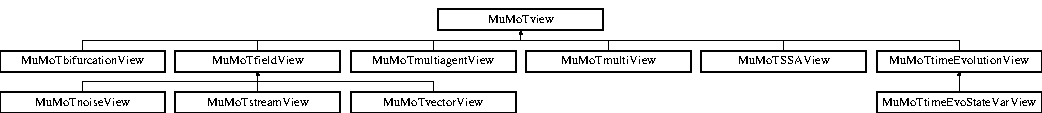
\includegraphics[height=1.521739cm]{class_mu_mo_t_1_1_mu_mo_t_1_1_mu_mo_tview}
\end{center}
\end{figure}
\subsection*{Public Member Functions}
\begin{DoxyCompactItemize}
\item 
def \hyperlink{class_mu_mo_t_1_1_mu_mo_t_1_1_mu_mo_tview_a367325b3bd7ca4a7b7ec4107f9aa6a16}{\+\_\+\+\_\+init\+\_\+\+\_\+} (self, model, controller, figure=None, params=None, kwargs)
\item 
def \hyperlink{class_mu_mo_t_1_1_mu_mo_t_1_1_mu_mo_tview_a64ca78b9bf9f0f3150077ab79405a674}{show\+Logs} (self, tail=False)
\end{DoxyCompactItemize}
\subsection*{Static Public Attributes}
\begin{DoxyCompactItemize}
\item 
\hyperlink{class_mu_mo_t_1_1_mu_mo_t_1_1_mu_mo_tview_afcc7a4b78ecd8fa7e713f8cfa0f51017}{value}
\item 
\hyperlink{class_mu_mo_t_1_1_mu_mo_t_1_1_mu_mo_tview_a2661f439a4a94ffdcd5e47ae1da0bb1d}{description}
\item 
\hyperlink{class_mu_mo_t_1_1_mu_mo_t_1_1_mu_mo_tview_a37d874d1d45bc2e5bfa013cddacb8e68}{logs} = self.\+\_\+single\+Run(random\+Seeds\mbox{[}i\mbox{]})
\item 
\hyperlink{class_mu_mo_t_1_1_mu_mo_t_1_1_mu_mo_tview_a69ffe654c8e97fdcbffcf35a1ded8157}{system\+Size} = sum(self.\+\_\+controller.\+\_\+view.\+\_\+initial\+State.\+values())
\begin{DoxyCompactList}\small\item\em Plot. \end{DoxyCompactList}\item 
\hyperlink{class_mu_mo_t_1_1_mu_mo_t_1_1_mu_mo_tview_aa820f7e11b025b06f4eeb0ad7581ad34}{max\+Time} = self.\+\_\+controller.\+\_\+widgets\+Extra\+Params\mbox{[}\textquotesingle{}max\+Time\textquotesingle{}\mbox{]}.\hyperlink{class_mu_mo_t_1_1_mu_mo_t_1_1_mu_mo_tview_afcc7a4b78ecd8fa7e713f8cfa0f51017}{value}
\item 
\hyperlink{class_mu_mo_t_1_1_mu_mo_t_1_1_mu_mo_tview_a23acc33d21869c517c7eb8114b3d8072}{pop}
\item 
\hyperlink{class_mu_mo_t_1_1_mu_mo_t_1_1_mu_mo_tview_a37dbdc30935031c05304482e1be89d8f}{color}
\item 
list \hyperlink{class_mu_mo_t_1_1_mu_mo_t_1_1_mu_mo_tview_a6a57a88c0fcb681f5721c6b1bce2dd96}{markers} = \mbox{[}plt.\+Line2D(\mbox{[}0,0\mbox{]},\mbox{[}0,0\mbox{]},\hyperlink{class_mu_mo_t_1_1_mu_mo_t_1_1_mu_mo_tview_a37dbdc30935031c05304482e1be89d8f}{color}=\hyperlink{class_mu_mo_t_1_1_mu_mo_t_1_1_mu_mo_tview_a37dbdc30935031c05304482e1be89d8f}{color}, marker=\textquotesingle{}\textquotesingle{}, linestyle=\textquotesingle{}-\/\textquotesingle{}) for \hyperlink{class_mu_mo_t_1_1_mu_mo_t_1_1_mu_mo_tview_a37dbdc30935031c05304482e1be89d8f}{color} in color\+Map.\+values()\mbox{]}
\item 
\hyperlink{class_mu_mo_t_1_1_mu_mo_t_1_1_mu_mo_tview_a411167eeca51189fabe03f884c7bf92c}{bbox\+\_\+to\+\_\+anchor}
\item 
\hyperlink{class_mu_mo_t_1_1_mu_mo_t_1_1_mu_mo_tview_aeee9f371db14fda0de35d16324a167df}{loc}
\item 
\hyperlink{class_mu_mo_t_1_1_mu_mo_t_1_1_mu_mo_tview_a15c45102c35a6e8e18adffce8cfdb703}{borderaxespad}
\end{DoxyCompactItemize}
\subsection*{Private Member Functions}
\begin{DoxyCompactItemize}
\item 
def \hyperlink{class_mu_mo_t_1_1_mu_mo_t_1_1_mu_mo_tview_a6822b561e2f9b618639714cd1545772e}{\+\_\+reset\+Error\+Message} (self)
\item 
def \hyperlink{class_mu_mo_t_1_1_mu_mo_t_1_1_mu_mo_tview_a23d2499d6c6334e35bc4cd7de3dd4d3c}{\+\_\+show\+Error\+Message} (self, message)
\item 
def \hyperlink{class_mu_mo_t_1_1_mu_mo_t_1_1_mu_mo_tview_abfc1e19ed53c088799d1f499bc010f7f}{\+\_\+set\+Log} (self, log)
\item 
def \hyperlink{class_mu_mo_t_1_1_mu_mo_t_1_1_mu_mo_tview_a8b4ffd0e4999bd45c6ca33fe0f40d1e3}{\+\_\+log} (self, analysis)
\item 
def \hyperlink{class_mu_mo_t_1_1_mu_mo_t_1_1_mu_mo_tview_a3af54c33f997937b14f422e772d5280a}{\+\_\+print\+\_\+standalone\+\_\+view\+\_\+cmd} (self)
\item 
def \hyperlink{class_mu_mo_t_1_1_mu_mo_t_1_1_mu_mo_tview_a36fe54d1f3a78f448ecd2a7eef8290d1}{\+\_\+get\+\_\+bookmarks\+\_\+params} (self)
\item 
def \hyperlink{class_mu_mo_t_1_1_mu_mo_t_1_1_mu_mo_tview_a118471f0e7fd4912146ed08084aa4b52}{\+\_\+build\+\_\+bookmark} (self)
\item 
def \hyperlink{class_mu_mo_t_1_1_mu_mo_t_1_1_mu_mo_tview_ab765afe539910b5869f0646dd4a5d915}{\+\_\+get\+Plot\+Limits} (self, default\+Limits=1)
\item 
def \hyperlink{class_mu_mo_t_1_1_mu_mo_t_1_1_mu_mo_tview_abee4df2eb2e49fa8bd5adc2b451b60df}{\+\_\+get\+System\+Size} (self, default\+Size=1)
\item 
def \hyperlink{class_mu_mo_t_1_1_mu_mo_t_1_1_mu_mo_tview_a145c99116673c6b90cc1b2d23e90af93}{\+\_\+get\+\_\+arg\+Dict} (self)
\begin{DoxyCompactList}\small\item\em gets and returns names and values from widgets \end{DoxyCompactList}\item 
def \hyperlink{class_mu_mo_t_1_1_mu_mo_t_1_1_mu_mo_tview_a89e6ad27bf7180f0dce5eb29527e8b73}{\+\_\+get\+\_\+fixed\+Points2d} (self)
\item 
def \hyperlink{class_mu_mo_t_1_1_mu_mo_t_1_1_mu_mo_tview_a52018bf4ba8d3fc732845a0a98b43b26}{\+\_\+get\+\_\+fixed\+Points3d} (self)
\begin{DoxyCompactList}\small\item\em calculates stationary states of 3d system \end{DoxyCompactList}\item 
def \hyperlink{class_mu_mo_t_1_1_mu_mo_t_1_1_mu_mo_tview_a4d4a00545816bf68f912f5ea5a449c48}{\+\_\+multirun} (self, iterations, random\+Seeds)
\item 
def \hyperlink{class_mu_mo_t_1_1_mu_mo_t_1_1_mu_mo_tview_a51d421aacb4cd83af5f1c2e60c3dff9c}{\+\_\+single\+Run} (self, random\+Seed)
\begin{DoxyCompactList}\small\item\em overwrite this method for views that allow the \textquotesingle{}multirun\textquotesingle{} command \end{DoxyCompactList}\end{DoxyCompactItemize}
\subsection*{Static Private Attributes}
\begin{DoxyCompactItemize}
\item 
\hyperlink{class_mu_mo_t_1_1_mu_mo_t_1_1_mu_mo_tview_aeacd9541246371f0db5cc3e3779762fa}{\+\_\+mumot\+Model} = None
\begin{DoxyCompactList}\small\item\em Model view is on. \end{DoxyCompactList}\item 
\hyperlink{class_mu_mo_t_1_1_mu_mo_t_1_1_mu_mo_tview_abf6d9f6be3898e307415d4598cde264d}{\+\_\+figure} = None
\begin{DoxyCompactList}\small\item\em Figure/axis object to plot view to. \end{DoxyCompactList}\item 
\hyperlink{class_mu_mo_t_1_1_mu_mo_t_1_1_mu_mo_tview_a5748371a5f2e09033908d21bb12f94c0}{\+\_\+figure\+Num} = None
\begin{DoxyCompactList}\small\item\em Unique figure number. \end{DoxyCompactList}\item 
\hyperlink{class_mu_mo_t_1_1_mu_mo_t_1_1_mu_mo_tview_a506ccaeadc9c6f4102cf4e06f5a6be2a}{\+\_\+axes3d} = None
\begin{DoxyCompactList}\small\item\em 3d axes? (False =$>$ 2d) \end{DoxyCompactList}\item 
\hyperlink{class_mu_mo_t_1_1_mu_mo_t_1_1_mu_mo_tview_a15f56ca9811d1e67d721fa64f9b0dc1e}{\+\_\+controller} = None
\begin{DoxyCompactList}\small\item\em Controller that controls this view. \end{DoxyCompactList}\item 
\hyperlink{class_mu_mo_t_1_1_mu_mo_t_1_1_mu_mo_tview_ac0ad5d0ca27f2668c0676334ee73ff52}{\+\_\+logs} = None
\begin{DoxyCompactList}\small\item\em Summary logs of view behaviour. \end{DoxyCompactList}\item 
\hyperlink{class_mu_mo_t_1_1_mu_mo_t_1_1_mu_mo_tview_ac7734326ac8dbbf9bd0d2c9838633195}{\+\_\+param\+Names} = None
\begin{DoxyCompactList}\small\item\em parameter names when used without controller \end{DoxyCompactList}\item 
\hyperlink{class_mu_mo_t_1_1_mu_mo_t_1_1_mu_mo_tview_a04608181fa27d9aad4983d3694f7ab17}{\+\_\+param\+Values} = None
\begin{DoxyCompactList}\small\item\em parameter values when used without controller \end{DoxyCompactList}\item 
\hyperlink{class_mu_mo_t_1_1_mu_mo_t_1_1_mu_mo_tview_a909146a3c119c927727c7d533042b184}{\+\_\+silent} = None
\begin{DoxyCompactList}\small\item\em silent flag (T\+R\+UE = do not try to acquire figure handle from pyplot) \end{DoxyCompactList}\item 
\hyperlink{class_mu_mo_t_1_1_mu_mo_t_1_1_mu_mo_tview_a590db9d889a22b57be41475d83d4d453}{\+\_\+plot\+Limits} = None
\begin{DoxyCompactList}\small\item\em plot limits (for non-\/constant system size) \end{DoxyCompactList}\item 
\hyperlink{class_mu_mo_t_1_1_mu_mo_t_1_1_mu_mo_tview_ace48ed03490093d8f44cde91e2f1e86e}{\+\_\+generating\+Command} = None
\begin{DoxyCompactList}\small\item\em command name that generates this view \end{DoxyCompactList}\item 
\hyperlink{class_mu_mo_t_1_1_mu_mo_t_1_1_mu_mo_tview_ad99375c41fba0adf5336e94457427ab2}{\+\_\+generating\+Kwargs} = None
\begin{DoxyCompactList}\small\item\em generating keyword arguments \end{DoxyCompactList}\end{DoxyCompactItemize}


\subsection{Detailed Description}
class describing a view on a model 

\subsection{Constructor \& Destructor Documentation}
\mbox{\Hypertarget{class_mu_mo_t_1_1_mu_mo_t_1_1_mu_mo_tview_a367325b3bd7ca4a7b7ec4107f9aa6a16}\label{class_mu_mo_t_1_1_mu_mo_t_1_1_mu_mo_tview_a367325b3bd7ca4a7b7ec4107f9aa6a16}} 
\index{Mu\+Mo\+T\+::\+Mu\+Mo\+T\+::\+Mu\+Mo\+Tview@{Mu\+Mo\+T\+::\+Mu\+Mo\+T\+::\+Mu\+Mo\+Tview}!\+\_\+\+\_\+init\+\_\+\+\_\+@{\+\_\+\+\_\+init\+\_\+\+\_\+}}
\index{\+\_\+\+\_\+init\+\_\+\+\_\+@{\+\_\+\+\_\+init\+\_\+\+\_\+}!Mu\+Mo\+T\+::\+Mu\+Mo\+T\+::\+Mu\+Mo\+Tview@{Mu\+Mo\+T\+::\+Mu\+Mo\+T\+::\+Mu\+Mo\+Tview}}
\subsubsection{\texorpdfstring{\+\_\+\+\_\+init\+\_\+\+\_\+()}{\_\_init\_\_()}}
{\footnotesize\ttfamily def \+\_\+\+\_\+init\+\_\+\+\_\+ (\begin{DoxyParamCaption}\item[{}]{self,  }\item[{}]{model,  }\item[{}]{controller,  }\item[{}]{figure = {\ttfamily None},  }\item[{}]{params = {\ttfamily None},  }\item[{}]{kwargs }\end{DoxyParamCaption})}



\subsection{Member Function Documentation}
\mbox{\Hypertarget{class_mu_mo_t_1_1_mu_mo_t_1_1_mu_mo_tview_a118471f0e7fd4912146ed08084aa4b52}\label{class_mu_mo_t_1_1_mu_mo_t_1_1_mu_mo_tview_a118471f0e7fd4912146ed08084aa4b52}} 
\index{Mu\+Mo\+T\+::\+Mu\+Mo\+T\+::\+Mu\+Mo\+Tview@{Mu\+Mo\+T\+::\+Mu\+Mo\+T\+::\+Mu\+Mo\+Tview}!\+\_\+build\+\_\+bookmark@{\+\_\+build\+\_\+bookmark}}
\index{\+\_\+build\+\_\+bookmark@{\+\_\+build\+\_\+bookmark}!Mu\+Mo\+T\+::\+Mu\+Mo\+T\+::\+Mu\+Mo\+Tview@{Mu\+Mo\+T\+::\+Mu\+Mo\+T\+::\+Mu\+Mo\+Tview}}
\subsubsection{\texorpdfstring{\+\_\+build\+\_\+bookmark()}{\_build\_bookmark()}}
{\footnotesize\ttfamily def \+\_\+build\+\_\+bookmark (\begin{DoxyParamCaption}\item[{}]{self }\end{DoxyParamCaption})\hspace{0.3cm}{\ttfamily [private]}}

\mbox{\Hypertarget{class_mu_mo_t_1_1_mu_mo_t_1_1_mu_mo_tview_a145c99116673c6b90cc1b2d23e90af93}\label{class_mu_mo_t_1_1_mu_mo_t_1_1_mu_mo_tview_a145c99116673c6b90cc1b2d23e90af93}} 
\index{Mu\+Mo\+T\+::\+Mu\+Mo\+T\+::\+Mu\+Mo\+Tview@{Mu\+Mo\+T\+::\+Mu\+Mo\+T\+::\+Mu\+Mo\+Tview}!\+\_\+get\+\_\+arg\+Dict@{\+\_\+get\+\_\+arg\+Dict}}
\index{\+\_\+get\+\_\+arg\+Dict@{\+\_\+get\+\_\+arg\+Dict}!Mu\+Mo\+T\+::\+Mu\+Mo\+T\+::\+Mu\+Mo\+Tview@{Mu\+Mo\+T\+::\+Mu\+Mo\+T\+::\+Mu\+Mo\+Tview}}
\subsubsection{\texorpdfstring{\+\_\+get\+\_\+arg\+Dict()}{\_get\_argDict()}}
{\footnotesize\ttfamily def \+\_\+get\+\_\+arg\+Dict (\begin{DoxyParamCaption}\item[{}]{self }\end{DoxyParamCaption})\hspace{0.3cm}{\ttfamily [private]}}



gets and returns names and values from widgets 

\mbox{\Hypertarget{class_mu_mo_t_1_1_mu_mo_t_1_1_mu_mo_tview_a36fe54d1f3a78f448ecd2a7eef8290d1}\label{class_mu_mo_t_1_1_mu_mo_t_1_1_mu_mo_tview_a36fe54d1f3a78f448ecd2a7eef8290d1}} 
\index{Mu\+Mo\+T\+::\+Mu\+Mo\+T\+::\+Mu\+Mo\+Tview@{Mu\+Mo\+T\+::\+Mu\+Mo\+T\+::\+Mu\+Mo\+Tview}!\+\_\+get\+\_\+bookmarks\+\_\+params@{\+\_\+get\+\_\+bookmarks\+\_\+params}}
\index{\+\_\+get\+\_\+bookmarks\+\_\+params@{\+\_\+get\+\_\+bookmarks\+\_\+params}!Mu\+Mo\+T\+::\+Mu\+Mo\+T\+::\+Mu\+Mo\+Tview@{Mu\+Mo\+T\+::\+Mu\+Mo\+T\+::\+Mu\+Mo\+Tview}}
\subsubsection{\texorpdfstring{\+\_\+get\+\_\+bookmarks\+\_\+params()}{\_get\_bookmarks\_params()}}
{\footnotesize\ttfamily def \+\_\+get\+\_\+bookmarks\+\_\+params (\begin{DoxyParamCaption}\item[{}]{self }\end{DoxyParamCaption})\hspace{0.3cm}{\ttfamily [private]}}

\mbox{\Hypertarget{class_mu_mo_t_1_1_mu_mo_t_1_1_mu_mo_tview_a89e6ad27bf7180f0dce5eb29527e8b73}\label{class_mu_mo_t_1_1_mu_mo_t_1_1_mu_mo_tview_a89e6ad27bf7180f0dce5eb29527e8b73}} 
\index{Mu\+Mo\+T\+::\+Mu\+Mo\+T\+::\+Mu\+Mo\+Tview@{Mu\+Mo\+T\+::\+Mu\+Mo\+T\+::\+Mu\+Mo\+Tview}!\+\_\+get\+\_\+fixed\+Points2d@{\+\_\+get\+\_\+fixed\+Points2d}}
\index{\+\_\+get\+\_\+fixed\+Points2d@{\+\_\+get\+\_\+fixed\+Points2d}!Mu\+Mo\+T\+::\+Mu\+Mo\+T\+::\+Mu\+Mo\+Tview@{Mu\+Mo\+T\+::\+Mu\+Mo\+T\+::\+Mu\+Mo\+Tview}}
\subsubsection{\texorpdfstring{\+\_\+get\+\_\+fixed\+Points2d()}{\_get\_fixedPoints2d()}}
{\footnotesize\ttfamily def \+\_\+get\+\_\+fixed\+Points2d (\begin{DoxyParamCaption}\item[{}]{self }\end{DoxyParamCaption})\hspace{0.3cm}{\ttfamily [private]}}

\mbox{\Hypertarget{class_mu_mo_t_1_1_mu_mo_t_1_1_mu_mo_tview_a52018bf4ba8d3fc732845a0a98b43b26}\label{class_mu_mo_t_1_1_mu_mo_t_1_1_mu_mo_tview_a52018bf4ba8d3fc732845a0a98b43b26}} 
\index{Mu\+Mo\+T\+::\+Mu\+Mo\+T\+::\+Mu\+Mo\+Tview@{Mu\+Mo\+T\+::\+Mu\+Mo\+T\+::\+Mu\+Mo\+Tview}!\+\_\+get\+\_\+fixed\+Points3d@{\+\_\+get\+\_\+fixed\+Points3d}}
\index{\+\_\+get\+\_\+fixed\+Points3d@{\+\_\+get\+\_\+fixed\+Points3d}!Mu\+Mo\+T\+::\+Mu\+Mo\+T\+::\+Mu\+Mo\+Tview@{Mu\+Mo\+T\+::\+Mu\+Mo\+T\+::\+Mu\+Mo\+Tview}}
\subsubsection{\texorpdfstring{\+\_\+get\+\_\+fixed\+Points3d()}{\_get\_fixedPoints3d()}}
{\footnotesize\ttfamily def \+\_\+get\+\_\+fixed\+Points3d (\begin{DoxyParamCaption}\item[{}]{self }\end{DoxyParamCaption})\hspace{0.3cm}{\ttfamily [private]}}



calculates stationary states of 3d system 

\mbox{\Hypertarget{class_mu_mo_t_1_1_mu_mo_t_1_1_mu_mo_tview_ab765afe539910b5869f0646dd4a5d915}\label{class_mu_mo_t_1_1_mu_mo_t_1_1_mu_mo_tview_ab765afe539910b5869f0646dd4a5d915}} 
\index{Mu\+Mo\+T\+::\+Mu\+Mo\+T\+::\+Mu\+Mo\+Tview@{Mu\+Mo\+T\+::\+Mu\+Mo\+T\+::\+Mu\+Mo\+Tview}!\+\_\+get\+Plot\+Limits@{\+\_\+get\+Plot\+Limits}}
\index{\+\_\+get\+Plot\+Limits@{\+\_\+get\+Plot\+Limits}!Mu\+Mo\+T\+::\+Mu\+Mo\+T\+::\+Mu\+Mo\+Tview@{Mu\+Mo\+T\+::\+Mu\+Mo\+T\+::\+Mu\+Mo\+Tview}}
\subsubsection{\texorpdfstring{\+\_\+get\+Plot\+Limits()}{\_getPlotLimits()}}
{\footnotesize\ttfamily def \+\_\+get\+Plot\+Limits (\begin{DoxyParamCaption}\item[{}]{self,  }\item[{}]{default\+Limits = {\ttfamily 1} }\end{DoxyParamCaption})\hspace{0.3cm}{\ttfamily [private]}}

\mbox{\Hypertarget{class_mu_mo_t_1_1_mu_mo_t_1_1_mu_mo_tview_abee4df2eb2e49fa8bd5adc2b451b60df}\label{class_mu_mo_t_1_1_mu_mo_t_1_1_mu_mo_tview_abee4df2eb2e49fa8bd5adc2b451b60df}} 
\index{Mu\+Mo\+T\+::\+Mu\+Mo\+T\+::\+Mu\+Mo\+Tview@{Mu\+Mo\+T\+::\+Mu\+Mo\+T\+::\+Mu\+Mo\+Tview}!\+\_\+get\+System\+Size@{\+\_\+get\+System\+Size}}
\index{\+\_\+get\+System\+Size@{\+\_\+get\+System\+Size}!Mu\+Mo\+T\+::\+Mu\+Mo\+T\+::\+Mu\+Mo\+Tview@{Mu\+Mo\+T\+::\+Mu\+Mo\+T\+::\+Mu\+Mo\+Tview}}
\subsubsection{\texorpdfstring{\+\_\+get\+System\+Size()}{\_getSystemSize()}}
{\footnotesize\ttfamily def \+\_\+get\+System\+Size (\begin{DoxyParamCaption}\item[{}]{self,  }\item[{}]{default\+Size = {\ttfamily 1} }\end{DoxyParamCaption})\hspace{0.3cm}{\ttfamily [private]}}

\mbox{\Hypertarget{class_mu_mo_t_1_1_mu_mo_t_1_1_mu_mo_tview_a8b4ffd0e4999bd45c6ca33fe0f40d1e3}\label{class_mu_mo_t_1_1_mu_mo_t_1_1_mu_mo_tview_a8b4ffd0e4999bd45c6ca33fe0f40d1e3}} 
\index{Mu\+Mo\+T\+::\+Mu\+Mo\+T\+::\+Mu\+Mo\+Tview@{Mu\+Mo\+T\+::\+Mu\+Mo\+T\+::\+Mu\+Mo\+Tview}!\+\_\+log@{\+\_\+log}}
\index{\+\_\+log@{\+\_\+log}!Mu\+Mo\+T\+::\+Mu\+Mo\+T\+::\+Mu\+Mo\+Tview@{Mu\+Mo\+T\+::\+Mu\+Mo\+T\+::\+Mu\+Mo\+Tview}}
\subsubsection{\texorpdfstring{\+\_\+log()}{\_log()}}
{\footnotesize\ttfamily def \+\_\+log (\begin{DoxyParamCaption}\item[{}]{self,  }\item[{}]{analysis }\end{DoxyParamCaption})\hspace{0.3cm}{\ttfamily [private]}}

\mbox{\Hypertarget{class_mu_mo_t_1_1_mu_mo_t_1_1_mu_mo_tview_a4d4a00545816bf68f912f5ea5a449c48}\label{class_mu_mo_t_1_1_mu_mo_t_1_1_mu_mo_tview_a4d4a00545816bf68f912f5ea5a449c48}} 
\index{Mu\+Mo\+T\+::\+Mu\+Mo\+T\+::\+Mu\+Mo\+Tview@{Mu\+Mo\+T\+::\+Mu\+Mo\+T\+::\+Mu\+Mo\+Tview}!\+\_\+multirun@{\+\_\+multirun}}
\index{\+\_\+multirun@{\+\_\+multirun}!Mu\+Mo\+T\+::\+Mu\+Mo\+T\+::\+Mu\+Mo\+Tview@{Mu\+Mo\+T\+::\+Mu\+Mo\+T\+::\+Mu\+Mo\+Tview}}
\subsubsection{\texorpdfstring{\+\_\+multirun()}{\_multirun()}}
{\footnotesize\ttfamily def \+\_\+multirun (\begin{DoxyParamCaption}\item[{}]{self,  }\item[{}]{iterations,  }\item[{}]{random\+Seeds }\end{DoxyParamCaption})\hspace{0.3cm}{\ttfamily [private]}}

\mbox{\Hypertarget{class_mu_mo_t_1_1_mu_mo_t_1_1_mu_mo_tview_a3af54c33f997937b14f422e772d5280a}\label{class_mu_mo_t_1_1_mu_mo_t_1_1_mu_mo_tview_a3af54c33f997937b14f422e772d5280a}} 
\index{Mu\+Mo\+T\+::\+Mu\+Mo\+T\+::\+Mu\+Mo\+Tview@{Mu\+Mo\+T\+::\+Mu\+Mo\+T\+::\+Mu\+Mo\+Tview}!\+\_\+print\+\_\+standalone\+\_\+view\+\_\+cmd@{\+\_\+print\+\_\+standalone\+\_\+view\+\_\+cmd}}
\index{\+\_\+print\+\_\+standalone\+\_\+view\+\_\+cmd@{\+\_\+print\+\_\+standalone\+\_\+view\+\_\+cmd}!Mu\+Mo\+T\+::\+Mu\+Mo\+T\+::\+Mu\+Mo\+Tview@{Mu\+Mo\+T\+::\+Mu\+Mo\+T\+::\+Mu\+Mo\+Tview}}
\subsubsection{\texorpdfstring{\+\_\+print\+\_\+standalone\+\_\+view\+\_\+cmd()}{\_print\_standalone\_view\_cmd()}}
{\footnotesize\ttfamily def \+\_\+print\+\_\+standalone\+\_\+view\+\_\+cmd (\begin{DoxyParamCaption}\item[{}]{self }\end{DoxyParamCaption})\hspace{0.3cm}{\ttfamily [private]}}

\mbox{\Hypertarget{class_mu_mo_t_1_1_mu_mo_t_1_1_mu_mo_tview_a6822b561e2f9b618639714cd1545772e}\label{class_mu_mo_t_1_1_mu_mo_t_1_1_mu_mo_tview_a6822b561e2f9b618639714cd1545772e}} 
\index{Mu\+Mo\+T\+::\+Mu\+Mo\+T\+::\+Mu\+Mo\+Tview@{Mu\+Mo\+T\+::\+Mu\+Mo\+T\+::\+Mu\+Mo\+Tview}!\+\_\+reset\+Error\+Message@{\+\_\+reset\+Error\+Message}}
\index{\+\_\+reset\+Error\+Message@{\+\_\+reset\+Error\+Message}!Mu\+Mo\+T\+::\+Mu\+Mo\+T\+::\+Mu\+Mo\+Tview@{Mu\+Mo\+T\+::\+Mu\+Mo\+T\+::\+Mu\+Mo\+Tview}}
\subsubsection{\texorpdfstring{\+\_\+reset\+Error\+Message()}{\_resetErrorMessage()}}
{\footnotesize\ttfamily def \+\_\+reset\+Error\+Message (\begin{DoxyParamCaption}\item[{}]{self }\end{DoxyParamCaption})\hspace{0.3cm}{\ttfamily [private]}}

\mbox{\Hypertarget{class_mu_mo_t_1_1_mu_mo_t_1_1_mu_mo_tview_abfc1e19ed53c088799d1f499bc010f7f}\label{class_mu_mo_t_1_1_mu_mo_t_1_1_mu_mo_tview_abfc1e19ed53c088799d1f499bc010f7f}} 
\index{Mu\+Mo\+T\+::\+Mu\+Mo\+T\+::\+Mu\+Mo\+Tview@{Mu\+Mo\+T\+::\+Mu\+Mo\+T\+::\+Mu\+Mo\+Tview}!\+\_\+set\+Log@{\+\_\+set\+Log}}
\index{\+\_\+set\+Log@{\+\_\+set\+Log}!Mu\+Mo\+T\+::\+Mu\+Mo\+T\+::\+Mu\+Mo\+Tview@{Mu\+Mo\+T\+::\+Mu\+Mo\+T\+::\+Mu\+Mo\+Tview}}
\subsubsection{\texorpdfstring{\+\_\+set\+Log()}{\_setLog()}}
{\footnotesize\ttfamily def \+\_\+set\+Log (\begin{DoxyParamCaption}\item[{}]{self,  }\item[{}]{log }\end{DoxyParamCaption})\hspace{0.3cm}{\ttfamily [private]}}

\mbox{\Hypertarget{class_mu_mo_t_1_1_mu_mo_t_1_1_mu_mo_tview_a23d2499d6c6334e35bc4cd7de3dd4d3c}\label{class_mu_mo_t_1_1_mu_mo_t_1_1_mu_mo_tview_a23d2499d6c6334e35bc4cd7de3dd4d3c}} 
\index{Mu\+Mo\+T\+::\+Mu\+Mo\+T\+::\+Mu\+Mo\+Tview@{Mu\+Mo\+T\+::\+Mu\+Mo\+T\+::\+Mu\+Mo\+Tview}!\+\_\+show\+Error\+Message@{\+\_\+show\+Error\+Message}}
\index{\+\_\+show\+Error\+Message@{\+\_\+show\+Error\+Message}!Mu\+Mo\+T\+::\+Mu\+Mo\+T\+::\+Mu\+Mo\+Tview@{Mu\+Mo\+T\+::\+Mu\+Mo\+T\+::\+Mu\+Mo\+Tview}}
\subsubsection{\texorpdfstring{\+\_\+show\+Error\+Message()}{\_showErrorMessage()}}
{\footnotesize\ttfamily def \+\_\+show\+Error\+Message (\begin{DoxyParamCaption}\item[{}]{self,  }\item[{}]{message }\end{DoxyParamCaption})\hspace{0.3cm}{\ttfamily [private]}}

\mbox{\Hypertarget{class_mu_mo_t_1_1_mu_mo_t_1_1_mu_mo_tview_a51d421aacb4cd83af5f1c2e60c3dff9c}\label{class_mu_mo_t_1_1_mu_mo_t_1_1_mu_mo_tview_a51d421aacb4cd83af5f1c2e60c3dff9c}} 
\index{Mu\+Mo\+T\+::\+Mu\+Mo\+T\+::\+Mu\+Mo\+Tview@{Mu\+Mo\+T\+::\+Mu\+Mo\+T\+::\+Mu\+Mo\+Tview}!\+\_\+single\+Run@{\+\_\+single\+Run}}
\index{\+\_\+single\+Run@{\+\_\+single\+Run}!Mu\+Mo\+T\+::\+Mu\+Mo\+T\+::\+Mu\+Mo\+Tview@{Mu\+Mo\+T\+::\+Mu\+Mo\+T\+::\+Mu\+Mo\+Tview}}
\subsubsection{\texorpdfstring{\+\_\+single\+Run()}{\_singleRun()}}
{\footnotesize\ttfamily def \+\_\+single\+Run (\begin{DoxyParamCaption}\item[{}]{self,  }\item[{}]{random\+Seed }\end{DoxyParamCaption})\hspace{0.3cm}{\ttfamily [private]}}



overwrite this method for views that allow the \textquotesingle{}multirun\textquotesingle{} command 

\mbox{\Hypertarget{class_mu_mo_t_1_1_mu_mo_t_1_1_mu_mo_tview_a64ca78b9bf9f0f3150077ab79405a674}\label{class_mu_mo_t_1_1_mu_mo_t_1_1_mu_mo_tview_a64ca78b9bf9f0f3150077ab79405a674}} 
\index{Mu\+Mo\+T\+::\+Mu\+Mo\+T\+::\+Mu\+Mo\+Tview@{Mu\+Mo\+T\+::\+Mu\+Mo\+T\+::\+Mu\+Mo\+Tview}!show\+Logs@{show\+Logs}}
\index{show\+Logs@{show\+Logs}!Mu\+Mo\+T\+::\+Mu\+Mo\+T\+::\+Mu\+Mo\+Tview@{Mu\+Mo\+T\+::\+Mu\+Mo\+T\+::\+Mu\+Mo\+Tview}}
\subsubsection{\texorpdfstring{show\+Logs()}{showLogs()}}
{\footnotesize\ttfamily def show\+Logs (\begin{DoxyParamCaption}\item[{}]{self,  }\item[{}]{tail = {\ttfamily False} }\end{DoxyParamCaption})}



\subsection{Field Documentation}
\mbox{\Hypertarget{class_mu_mo_t_1_1_mu_mo_t_1_1_mu_mo_tview_a506ccaeadc9c6f4102cf4e06f5a6be2a}\label{class_mu_mo_t_1_1_mu_mo_t_1_1_mu_mo_tview_a506ccaeadc9c6f4102cf4e06f5a6be2a}} 
\index{Mu\+Mo\+T\+::\+Mu\+Mo\+T\+::\+Mu\+Mo\+Tview@{Mu\+Mo\+T\+::\+Mu\+Mo\+T\+::\+Mu\+Mo\+Tview}!\+\_\+axes3d@{\+\_\+axes3d}}
\index{\+\_\+axes3d@{\+\_\+axes3d}!Mu\+Mo\+T\+::\+Mu\+Mo\+T\+::\+Mu\+Mo\+Tview@{Mu\+Mo\+T\+::\+Mu\+Mo\+T\+::\+Mu\+Mo\+Tview}}
\subsubsection{\texorpdfstring{\+\_\+axes3d}{\_axes3d}}
{\footnotesize\ttfamily \+\_\+axes3d = None\hspace{0.3cm}{\ttfamily [static]}, {\ttfamily [private]}}



3d axes? (False =$>$ 2d) 

\mbox{\Hypertarget{class_mu_mo_t_1_1_mu_mo_t_1_1_mu_mo_tview_a15f56ca9811d1e67d721fa64f9b0dc1e}\label{class_mu_mo_t_1_1_mu_mo_t_1_1_mu_mo_tview_a15f56ca9811d1e67d721fa64f9b0dc1e}} 
\index{Mu\+Mo\+T\+::\+Mu\+Mo\+T\+::\+Mu\+Mo\+Tview@{Mu\+Mo\+T\+::\+Mu\+Mo\+T\+::\+Mu\+Mo\+Tview}!\+\_\+controller@{\+\_\+controller}}
\index{\+\_\+controller@{\+\_\+controller}!Mu\+Mo\+T\+::\+Mu\+Mo\+T\+::\+Mu\+Mo\+Tview@{Mu\+Mo\+T\+::\+Mu\+Mo\+T\+::\+Mu\+Mo\+Tview}}
\subsubsection{\texorpdfstring{\+\_\+controller}{\_controller}}
{\footnotesize\ttfamily \+\_\+controller = None\hspace{0.3cm}{\ttfamily [static]}, {\ttfamily [private]}}



Controller that controls this view. 

\begin{DoxyRefDesc}{Todo}
\item[\hyperlink{todo__todo000026}{Todo}]
\begin{DoxyItemize}
\item could become None 
\end{DoxyItemize}\end{DoxyRefDesc}
\mbox{\Hypertarget{class_mu_mo_t_1_1_mu_mo_t_1_1_mu_mo_tview_abf6d9f6be3898e307415d4598cde264d}\label{class_mu_mo_t_1_1_mu_mo_t_1_1_mu_mo_tview_abf6d9f6be3898e307415d4598cde264d}} 
\index{Mu\+Mo\+T\+::\+Mu\+Mo\+T\+::\+Mu\+Mo\+Tview@{Mu\+Mo\+T\+::\+Mu\+Mo\+T\+::\+Mu\+Mo\+Tview}!\+\_\+figure@{\+\_\+figure}}
\index{\+\_\+figure@{\+\_\+figure}!Mu\+Mo\+T\+::\+Mu\+Mo\+T\+::\+Mu\+Mo\+Tview@{Mu\+Mo\+T\+::\+Mu\+Mo\+T\+::\+Mu\+Mo\+Tview}}
\subsubsection{\texorpdfstring{\+\_\+figure}{\_figure}}
{\footnotesize\ttfamily \+\_\+figure = None\hspace{0.3cm}{\ttfamily [static]}, {\ttfamily [private]}}



Figure/axis object to plot view to. 

\mbox{\Hypertarget{class_mu_mo_t_1_1_mu_mo_t_1_1_mu_mo_tview_a5748371a5f2e09033908d21bb12f94c0}\label{class_mu_mo_t_1_1_mu_mo_t_1_1_mu_mo_tview_a5748371a5f2e09033908d21bb12f94c0}} 
\index{Mu\+Mo\+T\+::\+Mu\+Mo\+T\+::\+Mu\+Mo\+Tview@{Mu\+Mo\+T\+::\+Mu\+Mo\+T\+::\+Mu\+Mo\+Tview}!\+\_\+figure\+Num@{\+\_\+figure\+Num}}
\index{\+\_\+figure\+Num@{\+\_\+figure\+Num}!Mu\+Mo\+T\+::\+Mu\+Mo\+T\+::\+Mu\+Mo\+Tview@{Mu\+Mo\+T\+::\+Mu\+Mo\+T\+::\+Mu\+Mo\+Tview}}
\subsubsection{\texorpdfstring{\+\_\+figure\+Num}{\_figureNum}}
{\footnotesize\ttfamily \+\_\+figure\+Num = None\hspace{0.3cm}{\ttfamily [static]}, {\ttfamily [private]}}



Unique figure number. 

\mbox{\Hypertarget{class_mu_mo_t_1_1_mu_mo_t_1_1_mu_mo_tview_ace48ed03490093d8f44cde91e2f1e86e}\label{class_mu_mo_t_1_1_mu_mo_t_1_1_mu_mo_tview_ace48ed03490093d8f44cde91e2f1e86e}} 
\index{Mu\+Mo\+T\+::\+Mu\+Mo\+T\+::\+Mu\+Mo\+Tview@{Mu\+Mo\+T\+::\+Mu\+Mo\+T\+::\+Mu\+Mo\+Tview}!\+\_\+generating\+Command@{\+\_\+generating\+Command}}
\index{\+\_\+generating\+Command@{\+\_\+generating\+Command}!Mu\+Mo\+T\+::\+Mu\+Mo\+T\+::\+Mu\+Mo\+Tview@{Mu\+Mo\+T\+::\+Mu\+Mo\+T\+::\+Mu\+Mo\+Tview}}
\subsubsection{\texorpdfstring{\+\_\+generating\+Command}{\_generatingCommand}}
{\footnotesize\ttfamily \+\_\+generating\+Command = None\hspace{0.3cm}{\ttfamily [static]}, {\ttfamily [private]}}



command name that generates this view 

\mbox{\Hypertarget{class_mu_mo_t_1_1_mu_mo_t_1_1_mu_mo_tview_ad99375c41fba0adf5336e94457427ab2}\label{class_mu_mo_t_1_1_mu_mo_t_1_1_mu_mo_tview_ad99375c41fba0adf5336e94457427ab2}} 
\index{Mu\+Mo\+T\+::\+Mu\+Mo\+T\+::\+Mu\+Mo\+Tview@{Mu\+Mo\+T\+::\+Mu\+Mo\+T\+::\+Mu\+Mo\+Tview}!\+\_\+generating\+Kwargs@{\+\_\+generating\+Kwargs}}
\index{\+\_\+generating\+Kwargs@{\+\_\+generating\+Kwargs}!Mu\+Mo\+T\+::\+Mu\+Mo\+T\+::\+Mu\+Mo\+Tview@{Mu\+Mo\+T\+::\+Mu\+Mo\+T\+::\+Mu\+Mo\+Tview}}
\subsubsection{\texorpdfstring{\+\_\+generating\+Kwargs}{\_generatingKwargs}}
{\footnotesize\ttfamily \+\_\+generating\+Kwargs = None\hspace{0.3cm}{\ttfamily [static]}, {\ttfamily [private]}}



generating keyword arguments 

\mbox{\Hypertarget{class_mu_mo_t_1_1_mu_mo_t_1_1_mu_mo_tview_ac0ad5d0ca27f2668c0676334ee73ff52}\label{class_mu_mo_t_1_1_mu_mo_t_1_1_mu_mo_tview_ac0ad5d0ca27f2668c0676334ee73ff52}} 
\index{Mu\+Mo\+T\+::\+Mu\+Mo\+T\+::\+Mu\+Mo\+Tview@{Mu\+Mo\+T\+::\+Mu\+Mo\+T\+::\+Mu\+Mo\+Tview}!\+\_\+logs@{\+\_\+logs}}
\index{\+\_\+logs@{\+\_\+logs}!Mu\+Mo\+T\+::\+Mu\+Mo\+T\+::\+Mu\+Mo\+Tview@{Mu\+Mo\+T\+::\+Mu\+Mo\+T\+::\+Mu\+Mo\+Tview}}
\subsubsection{\texorpdfstring{\+\_\+logs}{\_logs}}
{\footnotesize\ttfamily \+\_\+logs = None\hspace{0.3cm}{\ttfamily [static]}, {\ttfamily [private]}}



Summary logs of view behaviour. 

\mbox{\Hypertarget{class_mu_mo_t_1_1_mu_mo_t_1_1_mu_mo_tview_aeacd9541246371f0db5cc3e3779762fa}\label{class_mu_mo_t_1_1_mu_mo_t_1_1_mu_mo_tview_aeacd9541246371f0db5cc3e3779762fa}} 
\index{Mu\+Mo\+T\+::\+Mu\+Mo\+T\+::\+Mu\+Mo\+Tview@{Mu\+Mo\+T\+::\+Mu\+Mo\+T\+::\+Mu\+Mo\+Tview}!\+\_\+mumot\+Model@{\+\_\+mumot\+Model}}
\index{\+\_\+mumot\+Model@{\+\_\+mumot\+Model}!Mu\+Mo\+T\+::\+Mu\+Mo\+T\+::\+Mu\+Mo\+Tview@{Mu\+Mo\+T\+::\+Mu\+Mo\+T\+::\+Mu\+Mo\+Tview}}
\subsubsection{\texorpdfstring{\+\_\+mumot\+Model}{\_mumotModel}}
{\footnotesize\ttfamily \+\_\+mumot\+Model = None\hspace{0.3cm}{\ttfamily [static]}, {\ttfamily [private]}}



Model view is on. 

\mbox{\Hypertarget{class_mu_mo_t_1_1_mu_mo_t_1_1_mu_mo_tview_ac7734326ac8dbbf9bd0d2c9838633195}\label{class_mu_mo_t_1_1_mu_mo_t_1_1_mu_mo_tview_ac7734326ac8dbbf9bd0d2c9838633195}} 
\index{Mu\+Mo\+T\+::\+Mu\+Mo\+T\+::\+Mu\+Mo\+Tview@{Mu\+Mo\+T\+::\+Mu\+Mo\+T\+::\+Mu\+Mo\+Tview}!\+\_\+param\+Names@{\+\_\+param\+Names}}
\index{\+\_\+param\+Names@{\+\_\+param\+Names}!Mu\+Mo\+T\+::\+Mu\+Mo\+T\+::\+Mu\+Mo\+Tview@{Mu\+Mo\+T\+::\+Mu\+Mo\+T\+::\+Mu\+Mo\+Tview}}
\subsubsection{\texorpdfstring{\+\_\+param\+Names}{\_paramNames}}
{\footnotesize\ttfamily \+\_\+param\+Names = None\hspace{0.3cm}{\ttfamily [static]}, {\ttfamily [private]}}



parameter names when used without controller 

\mbox{\Hypertarget{class_mu_mo_t_1_1_mu_mo_t_1_1_mu_mo_tview_a04608181fa27d9aad4983d3694f7ab17}\label{class_mu_mo_t_1_1_mu_mo_t_1_1_mu_mo_tview_a04608181fa27d9aad4983d3694f7ab17}} 
\index{Mu\+Mo\+T\+::\+Mu\+Mo\+T\+::\+Mu\+Mo\+Tview@{Mu\+Mo\+T\+::\+Mu\+Mo\+T\+::\+Mu\+Mo\+Tview}!\+\_\+param\+Values@{\+\_\+param\+Values}}
\index{\+\_\+param\+Values@{\+\_\+param\+Values}!Mu\+Mo\+T\+::\+Mu\+Mo\+T\+::\+Mu\+Mo\+Tview@{Mu\+Mo\+T\+::\+Mu\+Mo\+T\+::\+Mu\+Mo\+Tview}}
\subsubsection{\texorpdfstring{\+\_\+param\+Values}{\_paramValues}}
{\footnotesize\ttfamily \+\_\+param\+Values = None\hspace{0.3cm}{\ttfamily [static]}, {\ttfamily [private]}}



parameter values when used without controller 

\mbox{\Hypertarget{class_mu_mo_t_1_1_mu_mo_t_1_1_mu_mo_tview_a590db9d889a22b57be41475d83d4d453}\label{class_mu_mo_t_1_1_mu_mo_t_1_1_mu_mo_tview_a590db9d889a22b57be41475d83d4d453}} 
\index{Mu\+Mo\+T\+::\+Mu\+Mo\+T\+::\+Mu\+Mo\+Tview@{Mu\+Mo\+T\+::\+Mu\+Mo\+T\+::\+Mu\+Mo\+Tview}!\+\_\+plot\+Limits@{\+\_\+plot\+Limits}}
\index{\+\_\+plot\+Limits@{\+\_\+plot\+Limits}!Mu\+Mo\+T\+::\+Mu\+Mo\+T\+::\+Mu\+Mo\+Tview@{Mu\+Mo\+T\+::\+Mu\+Mo\+T\+::\+Mu\+Mo\+Tview}}
\subsubsection{\texorpdfstring{\+\_\+plot\+Limits}{\_plotLimits}}
{\footnotesize\ttfamily \+\_\+plot\+Limits = None\hspace{0.3cm}{\ttfamily [static]}, {\ttfamily [private]}}



plot limits (for non-\/constant system size) 

\begin{DoxyRefDesc}{Todo}
\item[\hyperlink{todo__todo000027}{Todo}]\+: not used? \end{DoxyRefDesc}
\mbox{\Hypertarget{class_mu_mo_t_1_1_mu_mo_t_1_1_mu_mo_tview_a909146a3c119c927727c7d533042b184}\label{class_mu_mo_t_1_1_mu_mo_t_1_1_mu_mo_tview_a909146a3c119c927727c7d533042b184}} 
\index{Mu\+Mo\+T\+::\+Mu\+Mo\+T\+::\+Mu\+Mo\+Tview@{Mu\+Mo\+T\+::\+Mu\+Mo\+T\+::\+Mu\+Mo\+Tview}!\+\_\+silent@{\+\_\+silent}}
\index{\+\_\+silent@{\+\_\+silent}!Mu\+Mo\+T\+::\+Mu\+Mo\+T\+::\+Mu\+Mo\+Tview@{Mu\+Mo\+T\+::\+Mu\+Mo\+T\+::\+Mu\+Mo\+Tview}}
\subsubsection{\texorpdfstring{\+\_\+silent}{\_silent}}
{\footnotesize\ttfamily \+\_\+silent = None\hspace{0.3cm}{\ttfamily [static]}, {\ttfamily [private]}}



silent flag (T\+R\+UE = do not try to acquire figure handle from pyplot) 

\mbox{\Hypertarget{class_mu_mo_t_1_1_mu_mo_t_1_1_mu_mo_tview_a411167eeca51189fabe03f884c7bf92c}\label{class_mu_mo_t_1_1_mu_mo_t_1_1_mu_mo_tview_a411167eeca51189fabe03f884c7bf92c}} 
\index{Mu\+Mo\+T\+::\+Mu\+Mo\+T\+::\+Mu\+Mo\+Tview@{Mu\+Mo\+T\+::\+Mu\+Mo\+T\+::\+Mu\+Mo\+Tview}!bbox\+\_\+to\+\_\+anchor@{bbox\+\_\+to\+\_\+anchor}}
\index{bbox\+\_\+to\+\_\+anchor@{bbox\+\_\+to\+\_\+anchor}!Mu\+Mo\+T\+::\+Mu\+Mo\+T\+::\+Mu\+Mo\+Tview@{Mu\+Mo\+T\+::\+Mu\+Mo\+T\+::\+Mu\+Mo\+Tview}}
\subsubsection{\texorpdfstring{bbox\+\_\+to\+\_\+anchor}{bbox\_to\_anchor}}
{\footnotesize\ttfamily bbox\+\_\+to\+\_\+anchor\hspace{0.3cm}{\ttfamily [static]}}

\mbox{\Hypertarget{class_mu_mo_t_1_1_mu_mo_t_1_1_mu_mo_tview_a15c45102c35a6e8e18adffce8cfdb703}\label{class_mu_mo_t_1_1_mu_mo_t_1_1_mu_mo_tview_a15c45102c35a6e8e18adffce8cfdb703}} 
\index{Mu\+Mo\+T\+::\+Mu\+Mo\+T\+::\+Mu\+Mo\+Tview@{Mu\+Mo\+T\+::\+Mu\+Mo\+T\+::\+Mu\+Mo\+Tview}!borderaxespad@{borderaxespad}}
\index{borderaxespad@{borderaxespad}!Mu\+Mo\+T\+::\+Mu\+Mo\+T\+::\+Mu\+Mo\+Tview@{Mu\+Mo\+T\+::\+Mu\+Mo\+T\+::\+Mu\+Mo\+Tview}}
\subsubsection{\texorpdfstring{borderaxespad}{borderaxespad}}
{\footnotesize\ttfamily borderaxespad\hspace{0.3cm}{\ttfamily [static]}}

\mbox{\Hypertarget{class_mu_mo_t_1_1_mu_mo_t_1_1_mu_mo_tview_a37dbdc30935031c05304482e1be89d8f}\label{class_mu_mo_t_1_1_mu_mo_t_1_1_mu_mo_tview_a37dbdc30935031c05304482e1be89d8f}} 
\index{Mu\+Mo\+T\+::\+Mu\+Mo\+T\+::\+Mu\+Mo\+Tview@{Mu\+Mo\+T\+::\+Mu\+Mo\+T\+::\+Mu\+Mo\+Tview}!color@{color}}
\index{color@{color}!Mu\+Mo\+T\+::\+Mu\+Mo\+T\+::\+Mu\+Mo\+Tview@{Mu\+Mo\+T\+::\+Mu\+Mo\+T\+::\+Mu\+Mo\+Tview}}
\subsubsection{\texorpdfstring{color}{color}}
{\footnotesize\ttfamily color\hspace{0.3cm}{\ttfamily [static]}}

\mbox{\Hypertarget{class_mu_mo_t_1_1_mu_mo_t_1_1_mu_mo_tview_a2661f439a4a94ffdcd5e47ae1da0bb1d}\label{class_mu_mo_t_1_1_mu_mo_t_1_1_mu_mo_tview_a2661f439a4a94ffdcd5e47ae1da0bb1d}} 
\index{Mu\+Mo\+T\+::\+Mu\+Mo\+T\+::\+Mu\+Mo\+Tview@{Mu\+Mo\+T\+::\+Mu\+Mo\+T\+::\+Mu\+Mo\+Tview}!description@{description}}
\index{description@{description}!Mu\+Mo\+T\+::\+Mu\+Mo\+T\+::\+Mu\+Mo\+Tview@{Mu\+Mo\+T\+::\+Mu\+Mo\+T\+::\+Mu\+Mo\+Tview}}
\subsubsection{\texorpdfstring{description}{description}}
{\footnotesize\ttfamily description\hspace{0.3cm}{\ttfamily [static]}}

\mbox{\Hypertarget{class_mu_mo_t_1_1_mu_mo_t_1_1_mu_mo_tview_aeee9f371db14fda0de35d16324a167df}\label{class_mu_mo_t_1_1_mu_mo_t_1_1_mu_mo_tview_aeee9f371db14fda0de35d16324a167df}} 
\index{Mu\+Mo\+T\+::\+Mu\+Mo\+T\+::\+Mu\+Mo\+Tview@{Mu\+Mo\+T\+::\+Mu\+Mo\+T\+::\+Mu\+Mo\+Tview}!loc@{loc}}
\index{loc@{loc}!Mu\+Mo\+T\+::\+Mu\+Mo\+T\+::\+Mu\+Mo\+Tview@{Mu\+Mo\+T\+::\+Mu\+Mo\+T\+::\+Mu\+Mo\+Tview}}
\subsubsection{\texorpdfstring{loc}{loc}}
{\footnotesize\ttfamily loc\hspace{0.3cm}{\ttfamily [static]}}

\mbox{\Hypertarget{class_mu_mo_t_1_1_mu_mo_t_1_1_mu_mo_tview_a37d874d1d45bc2e5bfa013cddacb8e68}\label{class_mu_mo_t_1_1_mu_mo_t_1_1_mu_mo_tview_a37d874d1d45bc2e5bfa013cddacb8e68}} 
\index{Mu\+Mo\+T\+::\+Mu\+Mo\+T\+::\+Mu\+Mo\+Tview@{Mu\+Mo\+T\+::\+Mu\+Mo\+T\+::\+Mu\+Mo\+Tview}!logs@{logs}}
\index{logs@{logs}!Mu\+Mo\+T\+::\+Mu\+Mo\+T\+::\+Mu\+Mo\+Tview@{Mu\+Mo\+T\+::\+Mu\+Mo\+T\+::\+Mu\+Mo\+Tview}}
\subsubsection{\texorpdfstring{logs}{logs}}
{\footnotesize\ttfamily logs = self.\+\_\+single\+Run(random\+Seeds\mbox{[}i\mbox{]})\hspace{0.3cm}{\ttfamily [static]}}

\mbox{\Hypertarget{class_mu_mo_t_1_1_mu_mo_t_1_1_mu_mo_tview_a6a57a88c0fcb681f5721c6b1bce2dd96}\label{class_mu_mo_t_1_1_mu_mo_t_1_1_mu_mo_tview_a6a57a88c0fcb681f5721c6b1bce2dd96}} 
\index{Mu\+Mo\+T\+::\+Mu\+Mo\+T\+::\+Mu\+Mo\+Tview@{Mu\+Mo\+T\+::\+Mu\+Mo\+T\+::\+Mu\+Mo\+Tview}!markers@{markers}}
\index{markers@{markers}!Mu\+Mo\+T\+::\+Mu\+Mo\+T\+::\+Mu\+Mo\+Tview@{Mu\+Mo\+T\+::\+Mu\+Mo\+T\+::\+Mu\+Mo\+Tview}}
\subsubsection{\texorpdfstring{markers}{markers}}
{\footnotesize\ttfamily list markers = \mbox{[}plt.\+Line2D(\mbox{[}0,0\mbox{]},\mbox{[}0,0\mbox{]},\hyperlink{class_mu_mo_t_1_1_mu_mo_t_1_1_mu_mo_tview_a37dbdc30935031c05304482e1be89d8f}{color}=\hyperlink{class_mu_mo_t_1_1_mu_mo_t_1_1_mu_mo_tview_a37dbdc30935031c05304482e1be89d8f}{color}, marker=\textquotesingle{}\textquotesingle{}, linestyle=\textquotesingle{}-\/\textquotesingle{}) for \hyperlink{class_mu_mo_t_1_1_mu_mo_t_1_1_mu_mo_tview_a37dbdc30935031c05304482e1be89d8f}{color} in color\+Map.\+values()\mbox{]}\hspace{0.3cm}{\ttfamily [static]}}

\mbox{\Hypertarget{class_mu_mo_t_1_1_mu_mo_t_1_1_mu_mo_tview_aa820f7e11b025b06f4eeb0ad7581ad34}\label{class_mu_mo_t_1_1_mu_mo_t_1_1_mu_mo_tview_aa820f7e11b025b06f4eeb0ad7581ad34}} 
\index{Mu\+Mo\+T\+::\+Mu\+Mo\+T\+::\+Mu\+Mo\+Tview@{Mu\+Mo\+T\+::\+Mu\+Mo\+T\+::\+Mu\+Mo\+Tview}!max\+Time@{max\+Time}}
\index{max\+Time@{max\+Time}!Mu\+Mo\+T\+::\+Mu\+Mo\+T\+::\+Mu\+Mo\+Tview@{Mu\+Mo\+T\+::\+Mu\+Mo\+T\+::\+Mu\+Mo\+Tview}}
\subsubsection{\texorpdfstring{max\+Time}{maxTime}}
{\footnotesize\ttfamily max\+Time = self.\+\_\+controller.\+\_\+widgets\+Extra\+Params\mbox{[}\textquotesingle{}max\+Time\textquotesingle{}\mbox{]}.\hyperlink{class_mu_mo_t_1_1_mu_mo_t_1_1_mu_mo_tview_afcc7a4b78ecd8fa7e713f8cfa0f51017}{value}\hspace{0.3cm}{\ttfamily [static]}}

\mbox{\Hypertarget{class_mu_mo_t_1_1_mu_mo_t_1_1_mu_mo_tview_a23acc33d21869c517c7eb8114b3d8072}\label{class_mu_mo_t_1_1_mu_mo_t_1_1_mu_mo_tview_a23acc33d21869c517c7eb8114b3d8072}} 
\index{Mu\+Mo\+T\+::\+Mu\+Mo\+T\+::\+Mu\+Mo\+Tview@{Mu\+Mo\+T\+::\+Mu\+Mo\+T\+::\+Mu\+Mo\+Tview}!pop@{pop}}
\index{pop@{pop}!Mu\+Mo\+T\+::\+Mu\+Mo\+T\+::\+Mu\+Mo\+Tview@{Mu\+Mo\+T\+::\+Mu\+Mo\+T\+::\+Mu\+Mo\+Tview}}
\subsubsection{\texorpdfstring{pop}{pop}}
{\footnotesize\ttfamily pop\hspace{0.3cm}{\ttfamily [static]}}

\mbox{\Hypertarget{class_mu_mo_t_1_1_mu_mo_t_1_1_mu_mo_tview_a69ffe654c8e97fdcbffcf35a1ded8157}\label{class_mu_mo_t_1_1_mu_mo_t_1_1_mu_mo_tview_a69ffe654c8e97fdcbffcf35a1ded8157}} 
\index{Mu\+Mo\+T\+::\+Mu\+Mo\+T\+::\+Mu\+Mo\+Tview@{Mu\+Mo\+T\+::\+Mu\+Mo\+T\+::\+Mu\+Mo\+Tview}!system\+Size@{system\+Size}}
\index{system\+Size@{system\+Size}!Mu\+Mo\+T\+::\+Mu\+Mo\+T\+::\+Mu\+Mo\+Tview@{Mu\+Mo\+T\+::\+Mu\+Mo\+T\+::\+Mu\+Mo\+Tview}}
\subsubsection{\texorpdfstring{system\+Size}{systemSize}}
{\footnotesize\ttfamily system\+Size = sum(self.\+\_\+controller.\+\_\+view.\+\_\+initial\+State.\+values())\hspace{0.3cm}{\ttfamily [static]}}



Plot. 

\mbox{\Hypertarget{class_mu_mo_t_1_1_mu_mo_t_1_1_mu_mo_tview_afcc7a4b78ecd8fa7e713f8cfa0f51017}\label{class_mu_mo_t_1_1_mu_mo_t_1_1_mu_mo_tview_afcc7a4b78ecd8fa7e713f8cfa0f51017}} 
\index{Mu\+Mo\+T\+::\+Mu\+Mo\+T\+::\+Mu\+Mo\+Tview@{Mu\+Mo\+T\+::\+Mu\+Mo\+T\+::\+Mu\+Mo\+Tview}!value@{value}}
\index{value@{value}!Mu\+Mo\+T\+::\+Mu\+Mo\+T\+::\+Mu\+Mo\+Tview@{Mu\+Mo\+T\+::\+Mu\+Mo\+T\+::\+Mu\+Mo\+Tview}}
\subsubsection{\texorpdfstring{value}{value}}
{\footnotesize\ttfamily value\hspace{0.3cm}{\ttfamily [static]}}



The documentation for this class was generated from the following file\+:\begin{DoxyCompactItemize}
\item 
Mu\+Mo\+T/\hyperlink{_mu_mo_t_8py}{Mu\+Mo\+T.\+py}\end{DoxyCompactItemize}

\hypertarget{class_mu_mo_t_1_1_mu_mo_t_1_1_network_type}{}\section{Network\+Type Class Reference}
\label{class_mu_mo_t_1_1_mu_mo_t_1_1_network_type}\index{Network\+Type@{Network\+Type}}
Inheritance diagram for Network\+Type\+:\begin{figure}[H]
\begin{center}
\leavevmode
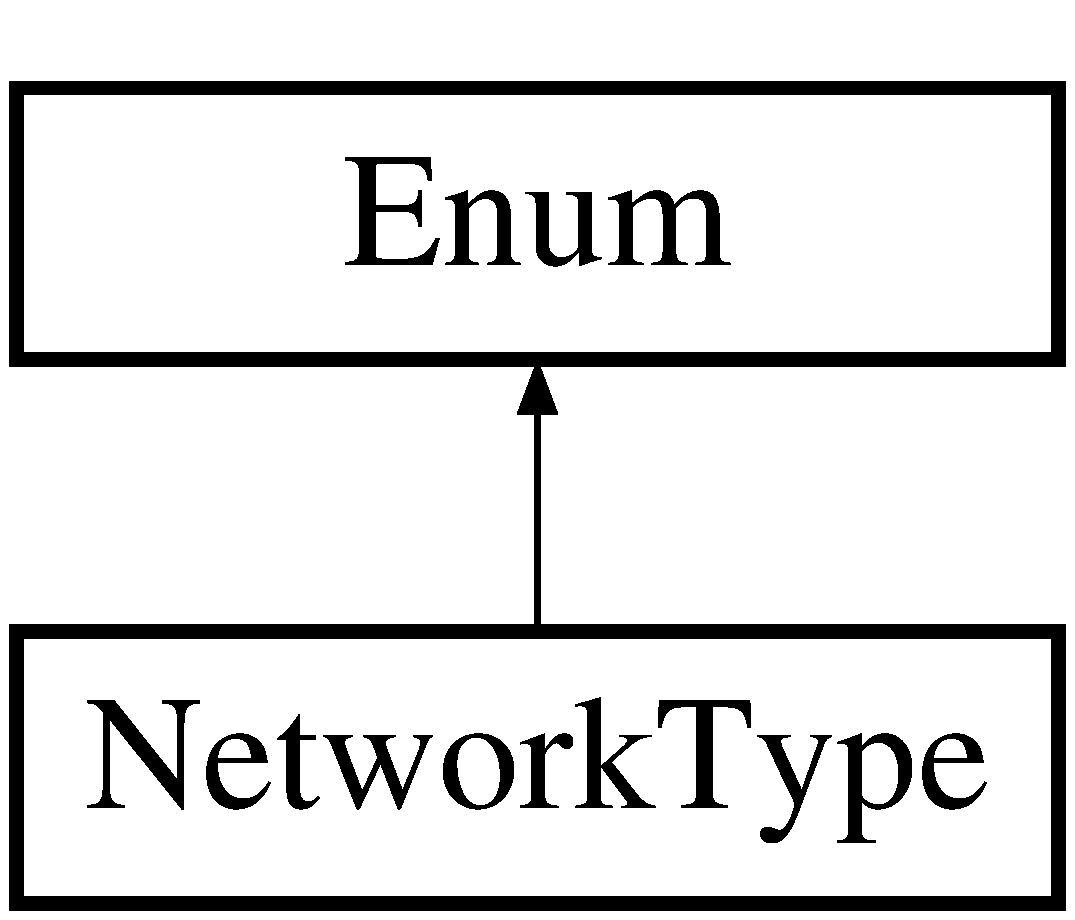
\includegraphics[height=2.000000cm]{class_mu_mo_t_1_1_mu_mo_t_1_1_network_type}
\end{center}
\end{figure}
\subsection*{Static Public Attributes}
\begin{DoxyCompactItemize}
\item 
int \hyperlink{class_mu_mo_t_1_1_mu_mo_t_1_1_network_type_a6026c1d0088de63c8dbffa271c5cb8e4}{F\+U\+L\+L\+Y\+\_\+\+C\+O\+N\+N\+E\+C\+T\+ED} = 0
\item 
int \hyperlink{class_mu_mo_t_1_1_mu_mo_t_1_1_network_type_abfc09d249fa8a7e47ccae49424a21d61}{E\+R\+S\+O\+S\+\_\+\+R\+E\+N\+YI} = 1
\item 
int \hyperlink{class_mu_mo_t_1_1_mu_mo_t_1_1_network_type_a5684807d763efd4f800fe9a849cd962c}{B\+A\+R\+A\+B\+A\+S\+I\+\_\+\+A\+L\+B\+E\+RT} = 2
\item 
int \hyperlink{class_mu_mo_t_1_1_mu_mo_t_1_1_network_type_a03813c265f977cc034eb42fd3370bf3d}{S\+P\+A\+CE} = 3
\item 
int \hyperlink{class_mu_mo_t_1_1_mu_mo_t_1_1_network_type_ad86080ad7b724db9fc31c1e654eba020}{D\+Y\+N\+A\+M\+IC} = 4
\end{DoxyCompactItemize}


\subsection{Field Documentation}
\mbox{\Hypertarget{class_mu_mo_t_1_1_mu_mo_t_1_1_network_type_a5684807d763efd4f800fe9a849cd962c}\label{class_mu_mo_t_1_1_mu_mo_t_1_1_network_type_a5684807d763efd4f800fe9a849cd962c}} 
\index{Mu\+Mo\+T\+::\+Mu\+Mo\+T\+::\+Network\+Type@{Mu\+Mo\+T\+::\+Mu\+Mo\+T\+::\+Network\+Type}!B\+A\+R\+A\+B\+A\+S\+I\+\_\+\+A\+L\+B\+E\+RT@{B\+A\+R\+A\+B\+A\+S\+I\+\_\+\+A\+L\+B\+E\+RT}}
\index{B\+A\+R\+A\+B\+A\+S\+I\+\_\+\+A\+L\+B\+E\+RT@{B\+A\+R\+A\+B\+A\+S\+I\+\_\+\+A\+L\+B\+E\+RT}!Mu\+Mo\+T\+::\+Mu\+Mo\+T\+::\+Network\+Type@{Mu\+Mo\+T\+::\+Mu\+Mo\+T\+::\+Network\+Type}}
\subsubsection{\texorpdfstring{B\+A\+R\+A\+B\+A\+S\+I\+\_\+\+A\+L\+B\+E\+RT}{BARABASI\_ALBERT}}
{\footnotesize\ttfamily int B\+A\+R\+A\+B\+A\+S\+I\+\_\+\+A\+L\+B\+E\+RT = 2\hspace{0.3cm}{\ttfamily [static]}}

\mbox{\Hypertarget{class_mu_mo_t_1_1_mu_mo_t_1_1_network_type_ad86080ad7b724db9fc31c1e654eba020}\label{class_mu_mo_t_1_1_mu_mo_t_1_1_network_type_ad86080ad7b724db9fc31c1e654eba020}} 
\index{Mu\+Mo\+T\+::\+Mu\+Mo\+T\+::\+Network\+Type@{Mu\+Mo\+T\+::\+Mu\+Mo\+T\+::\+Network\+Type}!D\+Y\+N\+A\+M\+IC@{D\+Y\+N\+A\+M\+IC}}
\index{D\+Y\+N\+A\+M\+IC@{D\+Y\+N\+A\+M\+IC}!Mu\+Mo\+T\+::\+Mu\+Mo\+T\+::\+Network\+Type@{Mu\+Mo\+T\+::\+Mu\+Mo\+T\+::\+Network\+Type}}
\subsubsection{\texorpdfstring{D\+Y\+N\+A\+M\+IC}{DYNAMIC}}
{\footnotesize\ttfamily int D\+Y\+N\+A\+M\+IC = 4\hspace{0.3cm}{\ttfamily [static]}}

\mbox{\Hypertarget{class_mu_mo_t_1_1_mu_mo_t_1_1_network_type_abfc09d249fa8a7e47ccae49424a21d61}\label{class_mu_mo_t_1_1_mu_mo_t_1_1_network_type_abfc09d249fa8a7e47ccae49424a21d61}} 
\index{Mu\+Mo\+T\+::\+Mu\+Mo\+T\+::\+Network\+Type@{Mu\+Mo\+T\+::\+Mu\+Mo\+T\+::\+Network\+Type}!E\+R\+S\+O\+S\+\_\+\+R\+E\+N\+YI@{E\+R\+S\+O\+S\+\_\+\+R\+E\+N\+YI}}
\index{E\+R\+S\+O\+S\+\_\+\+R\+E\+N\+YI@{E\+R\+S\+O\+S\+\_\+\+R\+E\+N\+YI}!Mu\+Mo\+T\+::\+Mu\+Mo\+T\+::\+Network\+Type@{Mu\+Mo\+T\+::\+Mu\+Mo\+T\+::\+Network\+Type}}
\subsubsection{\texorpdfstring{E\+R\+S\+O\+S\+\_\+\+R\+E\+N\+YI}{ERSOS\_RENYI}}
{\footnotesize\ttfamily int E\+R\+S\+O\+S\+\_\+\+R\+E\+N\+YI = 1\hspace{0.3cm}{\ttfamily [static]}}

\mbox{\Hypertarget{class_mu_mo_t_1_1_mu_mo_t_1_1_network_type_a6026c1d0088de63c8dbffa271c5cb8e4}\label{class_mu_mo_t_1_1_mu_mo_t_1_1_network_type_a6026c1d0088de63c8dbffa271c5cb8e4}} 
\index{Mu\+Mo\+T\+::\+Mu\+Mo\+T\+::\+Network\+Type@{Mu\+Mo\+T\+::\+Mu\+Mo\+T\+::\+Network\+Type}!F\+U\+L\+L\+Y\+\_\+\+C\+O\+N\+N\+E\+C\+T\+ED@{F\+U\+L\+L\+Y\+\_\+\+C\+O\+N\+N\+E\+C\+T\+ED}}
\index{F\+U\+L\+L\+Y\+\_\+\+C\+O\+N\+N\+E\+C\+T\+ED@{F\+U\+L\+L\+Y\+\_\+\+C\+O\+N\+N\+E\+C\+T\+ED}!Mu\+Mo\+T\+::\+Mu\+Mo\+T\+::\+Network\+Type@{Mu\+Mo\+T\+::\+Mu\+Mo\+T\+::\+Network\+Type}}
\subsubsection{\texorpdfstring{F\+U\+L\+L\+Y\+\_\+\+C\+O\+N\+N\+E\+C\+T\+ED}{FULLY\_CONNECTED}}
{\footnotesize\ttfamily int F\+U\+L\+L\+Y\+\_\+\+C\+O\+N\+N\+E\+C\+T\+ED = 0\hspace{0.3cm}{\ttfamily [static]}}

\mbox{\Hypertarget{class_mu_mo_t_1_1_mu_mo_t_1_1_network_type_a03813c265f977cc034eb42fd3370bf3d}\label{class_mu_mo_t_1_1_mu_mo_t_1_1_network_type_a03813c265f977cc034eb42fd3370bf3d}} 
\index{Mu\+Mo\+T\+::\+Mu\+Mo\+T\+::\+Network\+Type@{Mu\+Mo\+T\+::\+Mu\+Mo\+T\+::\+Network\+Type}!S\+P\+A\+CE@{S\+P\+A\+CE}}
\index{S\+P\+A\+CE@{S\+P\+A\+CE}!Mu\+Mo\+T\+::\+Mu\+Mo\+T\+::\+Network\+Type@{Mu\+Mo\+T\+::\+Mu\+Mo\+T\+::\+Network\+Type}}
\subsubsection{\texorpdfstring{S\+P\+A\+CE}{SPACE}}
{\footnotesize\ttfamily int S\+P\+A\+CE = 3\hspace{0.3cm}{\ttfamily [static]}}



The documentation for this class was generated from the following file\+:\begin{DoxyCompactItemize}
\item 
Mu\+Mo\+T/\hyperlink{_mu_mo_t_8py}{Mu\+Mo\+T.\+py}\end{DoxyCompactItemize}

\chapter{File Documentation}
\hypertarget{____init_____8py}{}\section{Mu\+Mo\+T/\+\_\+\+\_\+init\+\_\+\+\_\+.py File Reference}
\label{____init_____8py}\index{Mu\+Mo\+T/\+\_\+\+\_\+init\+\_\+\+\_\+.\+py@{Mu\+Mo\+T/\+\_\+\+\_\+init\+\_\+\+\_\+.\+py}}
\subsection*{Namespaces}
\begin{DoxyCompactItemize}
\item 
 \hyperlink{namespace_mu_mo_t}{Mu\+MoT}
\end{DoxyCompactItemize}

\hypertarget{_mu_mo_t_8py}{}\section{Mu\+Mo\+T.\+py File Reference}
\label{_mu_mo_t_8py}\index{Mu\+Mo\+T.\+py@{Mu\+Mo\+T.\+py}}
\subsection*{Data Structures}
\begin{DoxyCompactItemize}
\item 
class \hyperlink{class_mu_mo_t_1_1_network_type}{Network\+Type}
\item 
class \hyperlink{class_mu_mo_t_1_1_mu_mo_tdefault}{Mu\+Mo\+Tdefault}
\item 
class \hyperlink{class_mu_mo_t_1_1_mu_mo_tmodel}{Mu\+Mo\+Tmodel}
\begin{DoxyCompactList}\small\item\em class describing a model \end{DoxyCompactList}\item 
class \hyperlink{class_mu_mo_t_1_1___rule}{\+\_\+\+Rule}
\begin{DoxyCompactList}\small\item\em class describing a single reaction rule \end{DoxyCompactList}\item 
class \hyperlink{class_mu_mo_t_1_1_mu_mo_tcontroller}{Mu\+Mo\+Tcontroller}
\begin{DoxyCompactList}\small\item\em class describing a controller for a model view \end{DoxyCompactList}\item 
class \hyperlink{class_mu_mo_t_1_1_mu_mo_t_s_s_a_controller}{Mu\+Mo\+T\+S\+S\+A\+Controller}
\begin{DoxyCompactList}\small\item\em class describing a controller for multiagent views \end{DoxyCompactList}\item 
class \hyperlink{class_mu_mo_t_1_1_mu_mo_tmultiagent_controller}{Mu\+Mo\+Tmultiagent\+Controller}
\begin{DoxyCompactList}\small\item\em class describing a controller for multiagent views \end{DoxyCompactList}\item 
class \hyperlink{class_mu_mo_t_1_1_mu_mo_tview}{Mu\+Mo\+Tview}
\begin{DoxyCompactList}\small\item\em class describing a view on a model \end{DoxyCompactList}\item 
class \hyperlink{class_mu_mo_t_1_1_mu_mo_tmulti_view}{Mu\+Mo\+Tmulti\+View}
\begin{DoxyCompactList}\small\item\em multi-\/view view (tied closely to \hyperlink{class_mu_mo_t_1_1_mu_mo_tmulti_controller}{Mu\+Mo\+Tmulti\+Controller}) \end{DoxyCompactList}\item 
class \hyperlink{class_mu_mo_t_1_1_mu_mo_tmulti_controller}{Mu\+Mo\+Tmulti\+Controller}
\begin{DoxyCompactList}\small\item\em multi-\/view controller \end{DoxyCompactList}\item 
class \hyperlink{class_mu_mo_t_1_1_mu_mo_tfield_view}{Mu\+Mo\+Tfield\+View}
\begin{DoxyCompactList}\small\item\em field view on model (specialised by \hyperlink{class_mu_mo_t_1_1_mu_mo_tvector_view}{Mu\+Mo\+Tvector\+View} and \hyperlink{class_mu_mo_t_1_1_mu_mo_tstream_view}{Mu\+Mo\+Tstream\+View}) \end{DoxyCompactList}\item 
class \hyperlink{class_mu_mo_t_1_1_mu_mo_tstream_view}{Mu\+Mo\+Tstream\+View}
\begin{DoxyCompactList}\small\item\em stream plot view on model \end{DoxyCompactList}\item 
class \hyperlink{class_mu_mo_t_1_1_mu_mo_tvector_view}{Mu\+Mo\+Tvector\+View}
\begin{DoxyCompactList}\small\item\em vector plot view on model \end{DoxyCompactList}\item 
class \hyperlink{class_mu_mo_t_1_1_mu_mo_tbifurcation_view}{Mu\+Mo\+Tbifurcation\+View}
\begin{DoxyCompactList}\small\item\em bifurcation view on model \end{DoxyCompactList}\item 
class \hyperlink{class_mu_mo_t_1_1_mu_mo_tmultiagent_view}{Mu\+Mo\+Tmultiagent\+View}
\begin{DoxyCompactList}\small\item\em self.\+\_\+py\+D\+Scont.\+new\+Curve(self.\+\_\+py\+D\+Scont\+Args) self.\+\_\+py\+D\+Scont\mbox{[}\textquotesingle{}E\+Q1\textquotesingle{}\mbox{]}.reset(self.\+\_\+py\+D\+Smodel.\+pars) self.\+\_\+py\+D\+Sode.\+set(pars = self.\+\_\+py\+D\+Smodel.\+pars) self.\+\_\+py\+D\+Scont\mbox{[}\textquotesingle{}E\+Q1\textquotesingle{}\mbox{]}.reset() self.\+\_\+py\+D\+Scont.\+update(self.\+\_\+py\+D\+Scont\+Args) \#\# \end{DoxyCompactList}\item 
class \hyperlink{class_mu_mo_t_1_1_mu_mo_t_s_s_a_view}{Mu\+Mo\+T\+S\+S\+A\+View}
\begin{DoxyCompactList}\small\item\em agent on networks view on model \end{DoxyCompactList}\end{DoxyCompactItemize}
\subsection*{Namespaces}
\begin{DoxyCompactItemize}
\item 
 \hyperlink{namespace_mu_mo_t}{Mu\+MoT}
\end{DoxyCompactItemize}
\subsection*{Functions}
\begin{DoxyCompactItemize}
\item 
def \hyperlink{namespace_mu_mo_t_a563aad4a460dbcc0705cf99bb6f6dd5d}{parse\+Model} (model\+Description)
\begin{DoxyCompactList}\small\item\em create model from text description \end{DoxyCompactList}\item 
def \hyperlink{namespace_mu_mo_t_a276566fb102dd4e4bf32a9ba4fb8a09b}{\+\_\+derive\+O\+D\+Es\+From\+Rules} (reactants, rules)
\item 
def \hyperlink{namespace_mu_mo_t_a07dd350ff74bc1abafd7f44f972089a2}{\+\_\+raise\+Model\+Error} (expected, read, rule)
\item 
def \hyperlink{namespace_mu_mo_t_a4cf5ca1427b0999c933587bfaa89936d}{\+\_\+build\+Fig} (object, figure=None)
\begin{DoxyCompactList}\small\item\em generic method for constructing figures in \hyperlink{class_mu_mo_t_1_1_mu_mo_tview}{Mu\+Mo\+Tview} and \hyperlink{class_mu_mo_t_1_1_mu_mo_tmulti_controller}{Mu\+Mo\+Tmulti\+Controller} classes \end{DoxyCompactList}\end{DoxyCompactItemize}
\subsection*{Variables}
\begin{DoxyCompactItemize}
\item 
int \hyperlink{namespace_mu_mo_t_a4543afee285a2aa1cd5c8c9ca14fe77f}{figure\+Counter} = 1
\item 
int \hyperlink{namespace_mu_mo_t_ae8957aab30c8ae3e6065cd19d166ef22}{M\+A\+X\+\_\+\+R\+A\+N\+D\+O\+M\+\_\+\+S\+E\+ED} = 4294967295
\item 
float \hyperlink{namespace_mu_mo_t_aa168c4a595cabfd7f2af95bcc8c8636f}{I\+N\+I\+T\+I\+A\+L\+\_\+\+R\+A\+T\+E\+\_\+\+V\+A\+L\+UE} = 10.\+0
\item 
float \hyperlink{namespace_mu_mo_t_ad02e9bfc63846779b7b8c5aff0688879}{R\+A\+T\+E\+\_\+\+B\+O\+U\+ND} = 100.\+0
\item 
float \hyperlink{namespace_mu_mo_t_a62b44f6ef63c58313e64af86a7219285}{R\+A\+T\+E\+\_\+\+S\+T\+EP} = 0.\+1
\item 
int \hyperlink{namespace_mu_mo_t_a3911ed84a3973ff4c37bb3bd7d39f22d}{M\+U\+L\+T\+I\+P\+L\+O\+T\+\_\+\+C\+O\+L\+U\+M\+NS} = 2
\end{DoxyCompactItemize}

%--- End generated contents ---

% Index
\backmatter
\newpage
\phantomsection
\clearemptydoublepage
\addcontentsline{toc}{chapter}{Index}
\printindex

\end{document}
